%% Introduction
\begin{abstract}
  En este documento se va a tratar el diseño y especificación de \ac{VIMS},
  un proyecto de ingeniería que modela, diseña y arquitecta un sistema
  conformado por un dispositivo embebido y un servidor en la nube. El
  dispositivo se conecta al vehículo y transmite, mediante redes inalámbricas,
  los datos al servidor, que hará todo el procesamiento y gestión.
  El objetivo principal es devolverle al propietario del vehículo el control
  sobre el mismo, accediendo fácilmente a los datos recogidos por el automóvil
  así como de los mensajes de error.

  Para ello, primero se recogerán datos de una muestra de conductores y
  no conductores para identificar correctamente las necesidades de los
  usuarios y ajustar mejor el producto.
  
  A continuación, se elicitarán los requisitos que permitirán posteriormente
  modelar y diseñar el sistema de forma fiel. Esta fase permite trabajar
  directamente en los diagramas que modelan el sistema, tanto a nivel de
  casuísticas como en qué estructura deberá tener. Esto es fundamental porque
  simplificará y acotará las etapas de desarrollo posteriores.

  Además, se trabajará en el estudio del modelo matemático que permite traducir
  los datos recibidos por los vehículos según el estándar \ac{OBD}--II. A su vez,
  se estudiarán las características del sistema \textit{hardware} lo que permitirá
  desarrollar y construir una placa de control que será la encargada de gestionar los
  parámetros del dispositivo \ac{VIMS}.

  Por último, se estudian las distintas tareas en tiempo real que compondrán el sistema \ac{VIMS}
  mediante el análisis de tiempo de respuesta de las mismas. Dicho análisis
  determina la planificabilidad del sistema y asegura un correcto y predecible
  funcionamiento en cualquier circunstancia.
\end{abstract}

\selectlanguage{english}
\begin{abstract}
  \ac{VIMS} design and specification project is an integral engineering development
  which designs, models and architects a whole system built with an embedded
  device and a remote cloud server. The device is attached to the driver's vehicle
  and by using wireless communication transmits the data to the remote server,
  which handles the entire processing and data generation.
  The main objective is to bring the driver's sensation back of having control
  over the vehicle, easily accessing to the entire information it provides
  alongside error messages in an easy, accessible way.

  Firstly, a quest will be done so relevant data is collected from a sample
  of drivers and non-drivers which will help identifying their needs and
  better adjusting the final product.

  Then, the requirements will be elicited which will allow the modeling
  and the design of the system in further steps of the development.
  Such step allows working directly with the diagrams that will
  model the system in both behavioral and structural manners. This is
  crucial as it will simplify and delimit the next steps of the project.

  In addition, there will be a mathematical analysis on how to translate
  the data received from the vehicle itself into human-readable information,
  based on the \ac{OBD}--II standard. Furthermore, hardware characteristics
  will be studied which will allow developing and building a PCB which will
  handle the parameters of the \ac{VIMS} device.

  Finally, a real-time task analysis will be done for \ac{VIMS} system. This will lead us
  through the definition of the tasks themselves as well as the response time
  analysis for the whole system. Thus the analysis determines if the entire
  system can be scheduled asserting a well-known, correct behavior under any
  circumstances.
\end{abstract}

\selectlanguage{spanish}


\chapter{Introducción}\label{chap:intro}
En un mundo cada vez más interconectado, hay ciertas tecnologías que se quedan
por detrás en unos campos mientras que siguen progresando en otros. Esto se ve
directamente reflejado en la industria automovilística en donde los vehículos
cada vez cuentan con mayor y mejor tecnología (como cámaras, sensores, actuadores,
etc.) pero no es directamente accesible por el usuario: mediante pantallas e
interfaces se ofrecen métodos sencillos que facilitan su uso.

\ac{VIMS} pretende ser un sistema que facilite el acceso a todos los datos que
ofrece un vehículo para generar estadísticas, descubrir patrones en la conducción
y detectar errores. De esta forma, el conductor tendrá información de primera
mano sobre el estado de su vehículo, eficiencia de su conducción así como obtener
información en tiempo real complementaria a la ya propiciada por el vehículo.

\section{Estado del arte}\label{sec:state_of_the_art}
La historia de la automoción comienza estrictamente en el siglo XIX.
Un automóvil es, por definición, un vehículo que se mueve a sí mismo
(del griego, \textit{αὐτός} ``a sí mismo'' y del latín \textit{mobilis},
``que se mueve'').

Desde los primeros modelos como la serie T, de Ford, hasta el inicio de
la fabricación de vehículos por parte de Mercedes Benz, la historia del
automovilismo ha estado llena de grandes logros y avances en un intervalo
de tiempo relativamente pequeño (figura \ref{fig:ford_model_t}):

\begin{figure}[H]
  \centering
  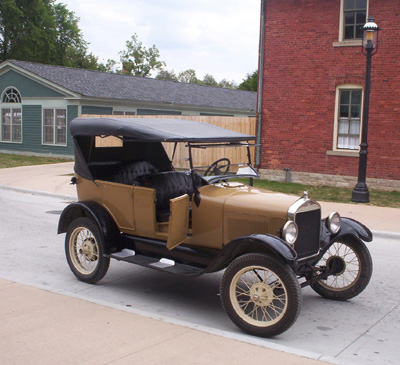
\includegraphics[width=.8\linewidth]{images/Late_model_Ford_Model_T.jpg}
  \caption{Ford modelo T del 1927 -- de Rmhermen \cite{Ford2022}.}
  \label{fig:ford_model_t}
\end{figure}

Durante aquella época, el ``mejor'' mecanismo de descubrimiento de
problemas era con algunos medidores y, sobre todo, por intuición:
sonidos del motor, olores extraños, \dots

No fue hasta los años 60 en donde los vehículos empezaron a incorporar
distintas interfaces con métricas que podían informar sobre el estado del
vehículo. El gran ``bum'' llegó con la expansión de la computadora, en donde
por primera vez se vio factible introducir un pequeño ordenador de 
abordo en el sistema.

En estos primeros sistemas, se incluyen indicadores del nivel de combustible,
sistema de refrigeración, presión del aceite, velocidad del motor,
temperatura del motor y otra información relativa al combustible. El
primer modelo que se conoce que incluye estos sistemas de cara a la
población en general es el Volkswagen Tipo III, en 1969 (figura \ref{fig:volkswagen_t3}):

\begin{figure}[H]
  \centering
  \includegraphics[width=.9\linewidth]{images/volkswagen_t3.jpg}
  \caption{Volkswagen Tipo III, modelo de inyección de 1969 -- de OSX - Trabajo propio \cite{VolkswagenTipo2021}.}
  \label{fig:volkswagen_t3}
\end{figure}

Pese a que supusieron un gran avance, estos primeros sistemas de
diagnóstico daban una información muy valiosa pero limitada, ya que muchos
diagnósticos seguirían siendo mediante los sentidos y las sensaciones
que le transmitiese el vehículo al mecánico. No fue hasta 1980 en donde
se implementó de forma estándar en los vehículos de \textit{General Motors}
el \ac{ALDL}, un lector de errores del coche que funcionó inicialmente a
160 baudios. Años más tarde, el sistema se refinaría usando el estándar
\ac{UART} \textit{half--duplex}, es decir, transmisión en los dos sentidos pero
no de forma simultánea (figura \ref{fig:aldl}). La principal motivación de incluir estos sistemas no fue
otra sino intentar reducir la contaminación de los vehículos teniendo
acceso a esta información \cite{SistemaOBD2Historia}.

\begin{figure}[H]
  \centering
  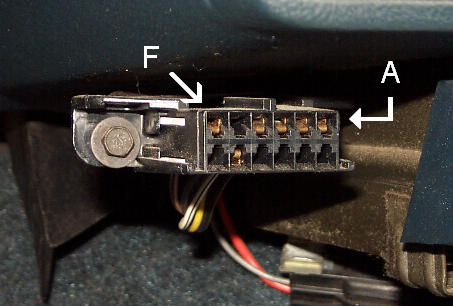
\includegraphics[width=.75\linewidth]{images/aldl.jpg}
  \caption{Conector \ac{ALDL}, creado por \textit{General Motors} antes de
  estandarizar OBD-II \cite{ReferenceManualChapter}.}
  \label{fig:aldl}
\end{figure}

No es hasta 1979 en que la \ac{SAE} recomienda crear un conector de
diagnóstico estandarizado en el mercado así como un conjunto de señales
de prueba. Finalmente, en 1991 la \ac{CARB} require que todos sus
vehículos tengan lo que sería el \ac{OBD}-I. Esta primera versión informaría
al conductor de un mal funcionamiento de alguno de los elementos del
vehículo mediante un \ac{MIL}, un indicador luminoso de fallos. Sin
embargo, solo se monitorizaban ciertos componentes relacionados con las
emisiones y no estaban calibrados \cite{SistemaOBD2Historia}.

Por ende, impulsado por las alertas \textit{smog} y por una fuerte regulación, en 1994
la \ac{CARB} obligó a todos los vehículos fabricados y vendidos a partir de 1996 incluir
el \ac{OBD}-II. Esto supuso un gran impulso en los mecanismos de monitorización de los
vehículos ya que además se estandarizó tanto el conector como los protocolos recomendados
por la \ac{SAE}. Tiempo más tarde, el Gobierno de los Estados Unidos aplicó la misma
medida a todos los vehículos del país \cite{SistemaOBD2Historia}.

Esta medida llegaría a Europa en 1998, según la Directiva 98/69EG, que obligaba a
todos los vehículos europeos a incluir dicho conector. Específicamente, los
automóviles de gasolina debían empezar a equiparlo en los modelos del año 2000; en el año 2003
para vehículos diésel; y en el año 2005 para camiones \cite{SistemaOBD2Historia}.

\subsection*{OBD--II}
\ac{OBD}--II es la segunda generación del sistema de diagnósticos de abordo, sucesor
de \ac{OBD}--I y su principal función es la de avisar al conductor cuando las
emisiones del vehículo son en torno a $1.5$ veces mayores de las diseñadas. A
diferencia de \ac{OBD}--I, \ac{OBD}--II también detecta fallos eléctricos, químicos
y mecánicos que puedan afectar al nivel de emisiones del vehículo (un caso típico
era un fallo químico del catalizador, indetectable por \ac{OBD}--I pero sí por la
segunda generación).

Este tipo de conector, al ser el primer estándar, cuenta con
múltiples interfaces que permiten conexiones mediante redes Wi-Fi, USB, Bluetooth,
etc. (cayendo pues en deshuso el protocolo de conexión por puerto serie -- RS232).
Esto se ha conseguido gracias al rápido avance de los sistemas embebidos, en donde
la combinación de \textit{software} y \textit{hardware} embebidos ha permitido que
cualquier usuario tenga acceso a este tipo de datos de forma relativamente simple
(actualmente, el conector más estandarizado es el controlador \texttt{ELM327} \cite{SistemaOBD2Historia},
figura \ref{fig:elm327}):

\begin{figure}[H]
  \centering
  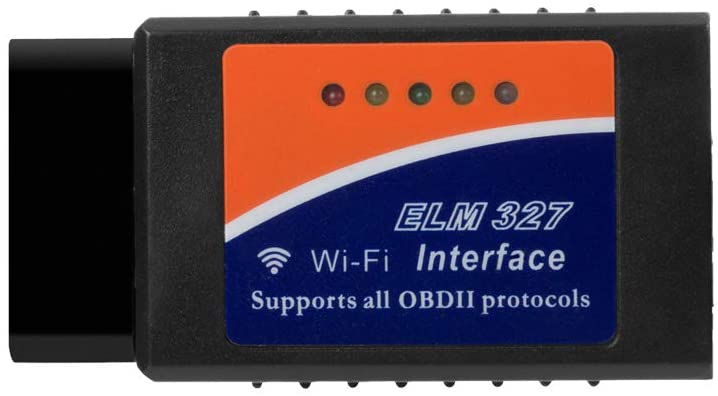
\includegraphics[width=.7\linewidth]{images/obd-ii-elm327.jpg}
  \caption{Controlador \texttt{ELM327} que cuenta con antenas Wi-Fi y Bluetooth para un acceso remoto \cite{AmazonComElm327}.}
  \label{fig:elm327}
\end{figure}

El sistema verifica todos los sensores directamente involucrados con las emisiones
del vehículo, como por ejemplo la inyección de aire al motor. Cuando algún sensor detecta
un fallo, se activa el \ac{MIL} indicando el fallo que sucede (o una combinación
de indicadores para notificar la existencia de un fallo, sin especificar exactamente
cuál).

El vehículo que incorpora un conector \ac{OBD}--II almacena la información sobre el
fallo del vehículo para que el mecánico que deba revisar el automóvil disponga de todos
los datos posibles. Por otra parte, este estándar permite una comunicación directa
con el vehículo mediante el envío de órdenes según un \ac{PID}. Por defecto, hay
una serie de \ac{PID}s estándar que la gran mayoría de vehículos deben incluir\footnote{%
Se dice ``la mayoría de vehículos'' porque hay ciertos \ac{PID}s que dependen
directamente del tipo de vehículo (a combustión, eléctrico, \dots) o del combustible
utilizado -- un vehículo eléctrico no ofrece información sobre las \ac{RPM} al igual
que un vehículo diésel no ofrece información sobre las bujías.}, pero también
los fabricantes de vehículos incluyen una serie de \ac{PID}s propios (conocidos como
\textit{\ac{PID}s propietarios}) que ofrecen información adaptada a cada vehículo
en particular y que, en principio, son privados y cerrados al público en general.

En Europa se implantó el \ac{EOBD}, la variación europea del estándar \ac{OBD}--II
implantada en el año 2000 en general. Si bien en apariencia es semejante al \ac{OBD}--II,
las diferencias radican en el \textit{software}. Por ejemplo, el estándar europeo
no monitoriza las evaporaciones del depósito de combustible; sin embargo, es más
sofisticado ya que usa ``mapas'' en las entradas de los sensores que obligan a que el
sensor se calibre empíricamente al sistema según las condiciones de operación del
motor (lo cual se traduce en que los sensores son mucho mejores pero más caros)
\cite{SistemaOBD2Historia}. Otra característica innovadora es que el sistema
europeo registra cuántos kilómetros se han recorrido desde que ha aparecido un
defecto \cite{EOBDOBD2}.

Finalmente, pero no menos importante, Japón tiene también su propio estándar denominado
\ac{JOBD}.

\subsection*{OBD--III}
El \ac{OBD}--III se espera que sea la siguiente versión del sistema que ya implementan
los coches actualmente. La principal diferencia con respecto a la versión anterior
será que el vehículo estará conectado de forma continua y emitiendo datos referentes
a las emisiones. De esta forma, se puede saber casi en el momento acerca de modificaciones
ilegales, un aumento en la contaminación del coche (signo de deterioro) y demás. No se
espera igualmente que sea un salto cualitativo ya que se sigue buscando que sea
altamente compatible con las herramientas que ya existen. Actualmente, se están
realizando pruebas en EE.UU. pero no hay cerrada ninguna fecha de estandarización
oficial por parte de los distintos continentes.

\subsection{Herramientas de monitorización y control del automóvil}
Pese al tiempo que lleva \ac{OBD}--II disponible, las herramientas existentes para
la actuación sobre un vehículo son relativamente escasas. La mayoría de modelos
presentes hoy en día en el mercado se basan directa o indirectamente en el
\texttt{ELM327}, un dispositivo de diagnóstico \ac{OBD} que cuenta con conexión
WiFi, Bluetooth y serie para la lectura local.

Por lo general, las herramientas que hay se utilizan por mecánicos o fanáticos del
sector para acceder a la información del estado del vehículo y ver los errores que
pudiera tener. Sin embargo, tras una breve documentación sobre el tema, la mayoría
de los casos buscaban directamente monitorizar en el momento el estado
del vehículo para obtener información relativa a los consumos, contaminación,
etc.

Por ejemplo, en el trabajo de Rimpas \textit{et al.} \cite{rimpasOBDIISensorDiagnostics2020}, se utiliza
un sensor \texttt{ELM327} para verificar que la información proporcionada por
el puerto del vehículo y la presentada por la telemetría presente en el mismo
(velocímetro y tacómetro) son coherentes entre sí (previa adaptación de los
valores en \textit{bytes} presentados por el conector a valores legibles). En
dicha investigación se llega a la conclusión de que el conector \ac{OBD}--II obtiene
valores fiables y consistentes tanto con los mostrados por el propio vehículo
como los proporcionados por el fabricante.

Otro tipo de investigaciones llevadas a cabo gracias a la presencia de este conector
en los automóviles es la de la caracterización de conductores y hábitos de conducción
según la telemetría reportada por el vehículo. En el estudio realizado por
Galih Hermawan y Emir Husni \cite{hermawanAcquisitionModelingEvaluating2020} se
estudia la combinación de la lectura de los sensores mediante el \ac{OBD}--II con
vehículos que presentan el sistema \ac{ADAS}.
El estudio busca identificar hábitos de conducción según la lectura de los diversos
sensores que hay en el sistema. También persigue detectar quién es el conductor que
está llevando el vehículo actualmente. En el estudio, el uso de \ac{OBD}--II junto
con los algoritmos de los \textit{k--Nearest Neighbor} (k--NN) y \textit{Naive Bayes}
consiguieron una precisión en la identificación del 100\% (
para un conjunto de datos de 10 conductores).
Por otra parte, el uso de inteligencia artificial junto con técnicas de \textit{clustering}
permitieron identificar comportamientos de los conductores al volante y relacionarlo
además con situaciones de riesgo y peligro. Además, se ha aplicado a otras características
también interesantes como detectar el tipo de calzada, predecir el tiempo de viaje,
analizar el consumo del vehículo y demás. El esquema seguido en la investigación es el
que se presenta en la figura \ref{fig:investigation-scheme}:

\begin{figure}[H]
  \centering
  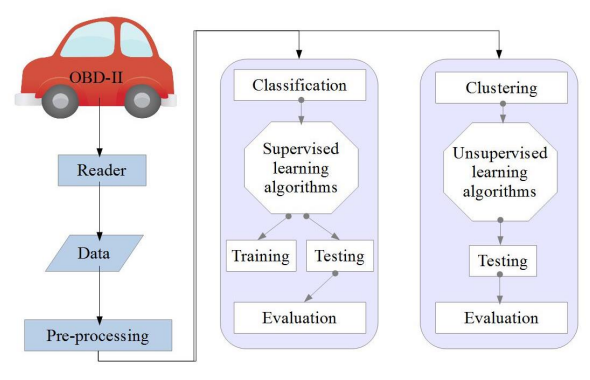
\includegraphics[width=.7\linewidth]{images/general-scheme-investigation.png}
  \caption{Esquema seguido para determinar los hábitos de conducción usando el \ac{OBD}--II \cite{hermawanAcquisitionModelingEvaluating2020}.}
  \label{fig:investigation-scheme}
\end{figure}

Por último, uno de los tipos de investigación bastante interesante realizada en los
últimos años es la de la generación de perfiles de conducción y de consumo. En el
artículo realizado por Ameen \textit{et al.} \cite{husseinaliameenDrivingBehaviourIdentification2021}
se define un sistema de clasificación del comportamiento del conductor al volante
(que es además el que se propone usar en este proyecto) el cual combina los datos
recibidos por el \ac{OBD}--II y del \ac{GPS} (figura \ref{fig:driving-behaviour}):

\begin{figure}[H]
  \centering
  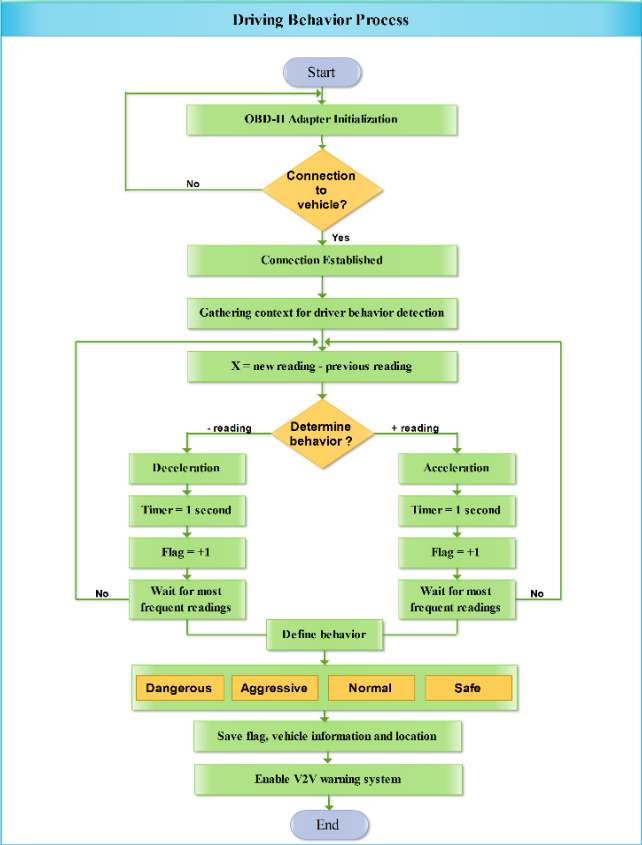
\includegraphics[width=.7\linewidth]{images/driving-behaviour-workflow.png}
  \caption{Flujo de análisis para determinar el comportamiento al volante de un conductor \cite{husseinaliameenDrivingBehaviourIdentification2021}.}
  \label{fig:driving-behaviour}
\end{figure}

Al final, el estudio concluía con los siguientes perfiles de conducción:

\begin{itemize}
  \item \textbf{Peligroso}, para una aceleración en general superior a $7\ \nicefrac{m}{s^2}$.
  \item \textbf{Agresivo}, para una aceleración entre $\left[4\ \nicefrac{m}{s^2}, 7\ \nicefrac{m}{s^2}\right)$.
  \item \textbf{Normal}, para una aceleración entre $\left[2\ \nicefrac{m}{s^2}, 4\ \nicefrac{m}{s^2}\right)$.
  \item \textbf{Seguro}, para una aceleración entre $\left[0\ \nicefrac{m}{s^2}, 2\ \nicefrac{m}{s^2}\right)$.
\end{itemize}

\section{Objetivos del desarrollo del proyecto}\label{sec:objectives}
Como se ha podido apreciar, existen multitud de aplicaciones relacionadas directa
o indirectamente con el \ac{OBD}--II, en parte por la longevidad del conector
en el mercado.

Sin embargo, todas o la gran mayoría de aplicaciones están destinadas a los profesionales
del sector, e incluso se ha aprovechado este conector para dificultar el acceso a
los datos del vehículo, habiendo de ir a un taller oficial para que puedan hacer
las reparaciones pertinentes.

Por otra parte, el parque de vehículos español es cada año más viejo debido a
diversos factores que no se van a analizar en este trabajo. Esto implica que cada
año más y más vehículos pierden el soporte por parte del fabricante y se vuelven
cada vez más costosos y complejos de mantener.

Para los no eruditos, el mundo del automóvil es el gran desconocido en donde una
serie de personas cualificadas se encargan del mantenimiento y correcto funcionamiento
del mecanismo que nos transporta por el mundo. Si bien es cierto que es necesaria
esta figura, hay una serie de buenas prácticas y actuaciones que pueden prevenir
tener que ir al mecánico de forma recurrente. Solo hace falta acceso a la información
de manera accesible.

Es por esto que nace \ac{VIMS}, un proyecto que pretende desarrollar un sistema completo
que consta de varias partes: un dispositivo embebido, un servidor y el usuario en sí
(figura \ref{fig:general-scheme}):

\begin{figure}[H]
  \centering
  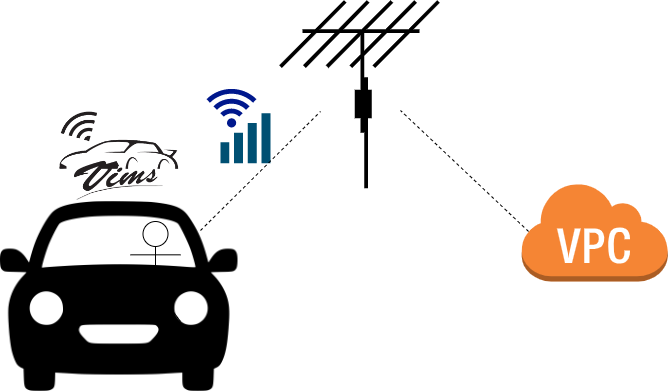
\includegraphics[width=\linewidth]{images/general-scheme.png}
  \caption{Esquema general que modela el modo de funcionamiento del sistema.}
  \label{fig:general-scheme}
\end{figure}

La idea fundamental detrás de este proyecto es la de devolverle a los usuarios
el control sobre su vehículo, ser conscientes de cómo funciona o, al menos, entender
mejor qué pueden hacer para mejorar tanto su estilo de conducción como la seguridad
al volante. De esta forma, con el dispositivo se espera también prevenir riesgos
ya que los propietarios y usuarios de los vehículos estarán informados en todo
momento de qué error pueda tener.

Como se prevé que este dispositivo sea utilizado por una gran variedad de usuarios
es crucial que sea accesible en términos de sencillez de manejo, entendimiento y
uso: evitar datos excesivamente técnicos, presentar la información más relevante
primero, etc.

Para ello, se hará uso de plataformas en la nube para gestionar, almacenar y presentar
la información al usuario y se contará con una aplicación móvil que permita un
fácil acceso a los datos del vehículo, tanto históricos como generados en el momento.

Al igual que otros trabajos previamente realizados, el proyecto se realiza sobre
las filosofías del código libre y del \textit{hardware} libre, que se traduce en
que todos los recursos (tanto físicos como \textit{software}) estarán disponibles
enteramente para cualquier persona interesada en ver cómo funciona, replicar el
proyecto por su cuenta y contar con plena potestad para mejorarlo, redistribuirlo
y trabajar con él (siempre bajo un prisma de reconocimiento al autor original
del trabajo regido por \textit{copyright}). Para ello, se ha decidido hacer uso
de la licencia MIT\footnote{Se pueden obtener más detalles sobre la licencia MIT
en la siguiente URL: \url{https://choosealicense.com/licenses/mit/}}.

\section{Metodología}\label{sec:methodology}
El proyecto que se pretende desarrollar es un proyecto de ingeniería. Esto se
traduce en que la metodología y la forma de trabajo son pilares fundamentales
en el desarrollo del mismo.

El primer paso realizado fue el de recopilar recursos e información de qué
necesitaban específicamente los usuarios. Para ello, se elaboró un cuestionario
en donde de forma general se preguntaba a conductores y no conductores qué querrían
tener en su vehículo. Los primeros sirvieron de grupo de control, los segundos para
aumentar la entropía de los datos obtenidos. El primer análisis realizado se detalla
en la sección \ref{ssec:user-req}, de la especificación de requisitos. Posteriormente,
en el punto \ref{chap:merch} se analiza en mayor profundidad los datos obtenidos
y se extraerán conclusiones.

A continuación, se realizó un estudio sobre qué plataformas y dispositivos están
accesibles de forma global para la generación y transmisión de datos. Esta fase
se centró principalmente en ``descubrir'' variantes del modelo ESP32 que incluyesen
ciertas antenas para permitir una mayor conectividad. Tras valorar diversas opciones,
se decidió usar el LILYGO T-SIM7000G ESP32 que incluye soporte de forma nativa para
tarjetas microSD, antena \ac{LTE}, alimentación externa por batería, antena \ac{GPS}, WiFi y
Bluetooth.

Una vez se decidió que dispositivo físico se iba a utilizar, se comenzó con el desarrollo
de los distintos diagramas que modelan el sistema, tanto lógicos como de diseño. Esta
parte fue crucial para asentar las bases de lo que será el proyecto y ha permitido seguir
el avance del mismo.

Por último, se realizó el serigrafiado de la placa y se comenzó la implementación
física de los diseños realizados. Sin embargo, esta etapa no se ha podido completar
por distintos contratiempos que se comentan en más detalle en el punto \ref{chap:planification}.


%% Product description
\chapter{Estructura del proyecto}\label{chap:structure}
El desarrollo del sistema \ac{VIMS} es un proceso multidisciplinar en el que se deben
desarrollar varias áreas de conocimiento. Este proyecto se ha postulado como
un desarrollo integral de ingeniería y es por eso por lo que está dividido en
varios bloques que conforman un factor clave en el desarrollo del mismo.

En este proyecto existen diversos bloques diferenciados: un estudio de mercado y de
las características de los usuarios, un estudio matemático asociado a la lectura de
valores y adecuación del \textit{hardware}, el proceso de diseño \textit{hardware}
en sí, el diseño \textit{software} del sistema y el análisis de planificación del mismo.

\begin{itemize}
  \item El estudio de mercado pretende averiguar y formalizar las necesidades de los
  conductores y usuarios de la vía. Es la primera aproximación y facilita la
  delimitación del producto y, sobre todo, ofrecerle al usuario final algo de utilidad
  y que pueda necesitar.
  \item El estudio matemático se encarga de investigar la ``traducción'' de los
  valores recibidos por el vehículo (según los datos asociados al estudio de mercado
  realizado con anterioridad).
  \item El diseño \textit{software} modela principalmente cómo se va a estructurar
  el sistema y cómo debe comportarse ante los distintos eventos que puede recibir.
  Esta fase conlleva realizar diagramas lógicos y de diseño del sistema en su conjunto.
  \item El diseño \textit{hardware} conlleva tanto el estudio de los componentes del
  sistema así como de las restricciones físicas del mismo. Además, en esta sección
  también se introduce el diseño 3D de la caja que alojará la placa.
  \item El análisis de planificabilidad complementa el diseño \textit{software}
  y estudia si el sistema es planificable. En los requisitos no se define \ac{VIMS}
  como un sistema en tiempo real, pero la cantidad de componentes que contiene y las
  acciones que tiene que realizar requieren del uso de subrutinas y de una planificación
  previa para asegurar un correcto funcionamiento del mismo.
\end{itemize}

Es importante detallar que pese a que el sistema se compone de varios componentes,
son dos los principales que lo caracterizan:

\begin{enumerate}
  \item La placa, \ac{VIMS}, que va embebida en los vehículos del sistema. Se encarga
  de toda la lectura, adaptación y emisión de datos. Además, cuenta con soporte para
  poder realizar una transmisión de la información a un dispositivo asociado mediante
  redes \ac{PAN}.
  \item El servidor \textit{cloud}, el ``cerebro'' encargado de recibir las tramas,
  los datos y la información relativa a las placas \ac{VIMS}, los dispositivos de
  usuario y demás componentes. Además, tiene la responsabilidad de ofrecer a los
  usuarios una \ac{GUI}, generar información relevante a partir de los datos (como
  estadísticas), gestionar las suscripciones y enviar periódicamente la información
  al usuario.
\end{enumerate}

\section{Estudio de mercado}\label{sec:merch}
Para el desarrollo de este proyecto, se hizo un estudio de mercado tanto de los
consumidores como de sus características, además de una evaluación exhaustiva
de qué les gustaría tener en su vehículo.

Este proyecto pretende en un futuro salir a mercado y suplir características que los
usuarios echan en falta en sus correspondientes medios de transporte. Como en principio
funciona con cualquier vehículo que cuente con \ac{OBD}--II, las respuestas no se han
limitado a aquellos conductores que condujesen turismos sino cualquier tipo de
automóvil: motocicleta, camión, etc.

Es importante destacar que el estudio tiene varios sesgos que han restringido
y delimitado las respuestas que se han registrado:

\begin{enumerate}
  \item Se ha realizado un cuestionario usando Google Forms, una plataforma de Google
        que permite preparar una serie de preguntas y respuestas y aplicar ciertos
        filtros sobre ellas. Por ejemplo, para aquellos que dijeron ser conductores,
        se hicieron preguntas diferentes frente a quienes no lo fueran.

        Esto permite obtener datos más fidedignos y acotados según la población que
        respondiera. Sin embargo, tiene una limitación implícita: restringe el acceso
        a aquellos con conocimientos ``suficientes'' acerca de la plataforma. Pese
        a que el producto pretende ser lo más accesible posible, no hay que olvidar
        que este tipo de tecnologías permanecen desconocidas para una gran parte
        de la población con escasos conocimientos acerca de Internet o de las
        nuevas tecnologías. Se comentará más adelante, pero esto se ve reflejado
        principalmente en la edad media de quienes respondieron el cuestionario.

        Por otra parte, al ser un cuestionario aparece otra limitación implícita
        y es la validación y verificación de las respuestas: se confía en la buena
        fe de los participantes y en la calidad de sus respuestas. Igualmente, se
        desarrolló el cuestionario junto con una psicóloga que ayudó a definir
        preguntas cerradas e incluir ciertas respuestas de control. Por otra parte,
        se usó el propio mecanismo que ofrece este servicio de Google para ordenar
        aleatoriamente las respuestas del cuestionario (y que eso sirviese también
        como control).

  \item Los encuestados fueron contactados principalmente por la red social Twitter,
        mediante la difusión con ``me gusta'' y ``retweet''. También se usaron otros
        medios de comunicación (como el correo UPM y Telegram/WhatsApp), pero el
        mayoritario fue el ya mencionado. Nuevamente, esto introduce un sesgo tanto
        por edad como por accesibilidad.

  \item Junto con la encuesta, se realizó un sorteo entre aquellos que respondiesen
        a la misma de un cheque regalo de Amazon valorado en 20\EUR{}. Si bien este
        incentivo pudiera resultar interesante, puede resultar también en un nuevo
        sesgo en donde personas que o bien no compren en Amazon o bien no sepan
        lo que es no quisieran hacer el cuestionario.

        Además, se plantea la casuística en que ciertas personas quisieran responder
        al cuestionario solo por el cheque de Amazon, sin importar la calidad de
        las respuestas, ``ensuciando'' los resultados obtenidos y quitándole credibilidad
        al cuestionario en sí.

        Esto se analizará posteriormente junto con las respuestas recibidas y las
        preguntas de control introducidas.

  \item El cuestionario, al ser relativamente exhaustivo, pudo echar para atrás a muchos
        posibles encuestados ya que se estima que el tiempo medio para realizarlo es del
        orden de 10/15 minutos. A parte del daño evidente de tener menos muestra con la
        que trabajar, este posible suceso reduciría también la variedad de la población
        y la calidad del estudio realizado.
\end{enumerate}

La primera pregunta que se realizó a los encuestados era si eran conductores o no.
Los datos revelan que el $72.7\%$ ($16$) de los encuestados son conductores, mientras que el
$27.3\%$ ($6$) restantes no, del total que fueron $22$ (figura \ref{fig:drivers-nodrivers}):

\begin{figure}[H]
  \centering
  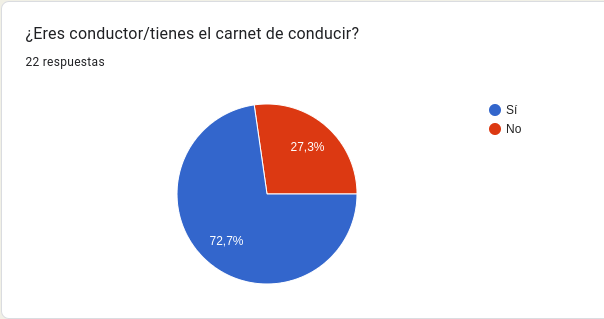
\includegraphics[width=\linewidth]{images/drivers-nodrivers.png}
  \caption{Gráfico de tarta que muestra quiénes de los encuestados son conductores ($72.7\%$) y quiénes no ($27.3\%$).}
  \label{fig:drivers-nodrivers}
\end{figure}

Sobre aquellos que dijeron ser conductores, se preguntó acerca de los años que
llevaban con carnet de conducir, así como los tipos de carnet de conducir que tenían
los encuestados.

Se vio que un $68.8\%$ tenía el carnet desde hace 3 años o más ($11$ encuestados
en particular); un $12.5\%$ tenía el carnet desde hace solo un año ($2$ encuestados)
y el restante, en su mayoría, tenía el carnet desde hace menos de un año. Esto se ve
reflejado en el histograma \ref{fig:carnet-time-hist}:

\begin{figure}[H]
  \centering
  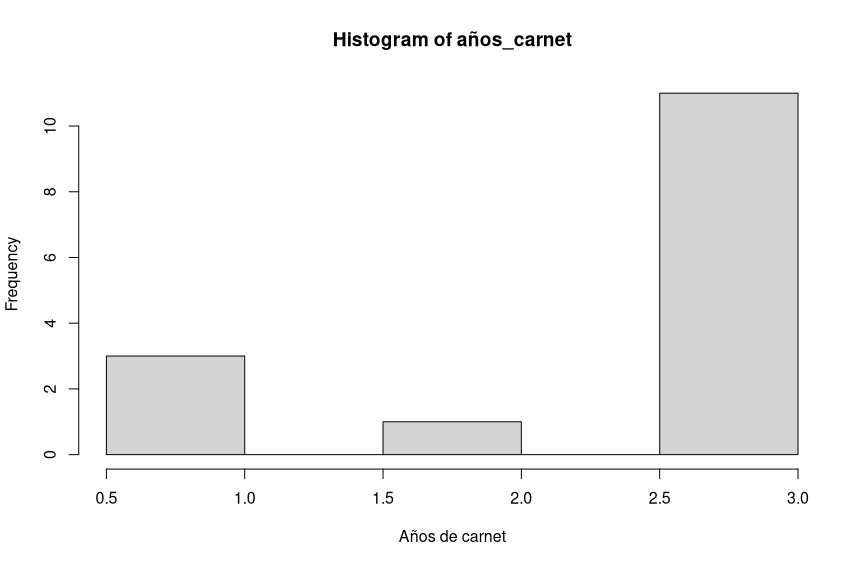
\includegraphics[width=\linewidth]{images/carnet-time.png}
  \caption{Histograma que muestra los años de carnet de los encuestados.}
  \label{fig:carnet-time-hist}
\end{figure}

Con respecto a los tipos de carnet, el $100\%$ de los encuestados (que dijeron ser
conductores) tiene el carnet tipo B. Se vio además que el $18.8\%$ tiene además los
carnets relativos a las motocicletas (muy posiblemente, los encuestados tienen el
carnet tipo ``A'' que les habilita automáticamente para aquellos de menor nivel,
como el AM, A1 y A2); y únicamente un encuestado tiene el carnet tipo C, que permite
conducir camiones.

Una restricción que se comentó con anterioridad era la edad media de los participantes.
Esta pregunta se realizó por dos motivos:

\begin{enumerate}
  \item Definir estadísticamente la edad media de la población para una posterior evaluación
        de su longevidad y experiencia tanto en la conducción como en la posible
        compra-venta de vehículos.
  \item Diferenciar, definir y clasificar los encuestados por grupos de edad y descubrir
        posibles sesgos y restricciones en las respuestas para un posterior análisis
        sobre la causa de dichos sesgos y restricciones.
\end{enumerate}

Es necesario decir que solo se preguntó por la edad a aquellas personas que respondieron
afirmativamente a ser conductores. Esto se hizo así debido a que sus respuestas han
conformado el dato más relativo a la hora de realizar la investigación, y se hace así
también estadísticamente.

Se tiene pues que:

\begin{equation}\label{eq:ages}
  \left\{\begin{aligned}
    X_{min}               & = 19     \\
    \bar{X}               & = 30     \\
    Mediana\left(X\right) & = 26.5   \\
    S\left(X\right)       & = 10.564 \\
    X_{max}               & = 55
  \end{aligned}\right.
\end{equation}

Se construyó además un gráfico de tarta (figura \ref{fig:ages}) que muestra cómo
quedan distribuidas las edades de los participantes:

\begin{figure}[H]
  \centering
  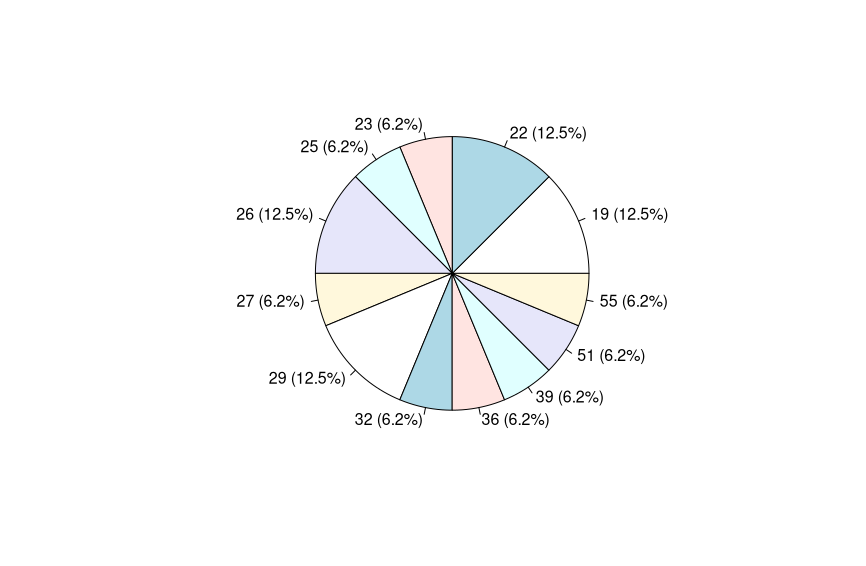
\includegraphics[width=\linewidth]{images/ages-pie.png}
  \caption{Gráfico de tarta que muestra la distribución de edades (valor previo al paréntesis) y su frecuencia en porcentaje.}
  \label{fig:ages}
\end{figure}

Como se puede ver en la ecuación \ref{eq:ages}, la distancia entre los valores
mínimo y máximo es de $36$ puntos. Sin embargo, los valores de la media $\left(\bar{X}\right)$
y la mediana $\left(Mediana\left(X\right)\right)$ muestran que la distribución está
bastante centrada en torno a la media, con una desviación estándar $\left(S\left(X\right)\right)$
de $\approx\pm10.564$.

Es interesante notar los tres grandes bloques presentes en la figura \ref{fig:ages}
que evidencian lo que se venía indicando anteriormente: en proporción, a la encuesta
ha accedido más población joven que adulta. Mismamente, solo el porcentaje de personas
encuestadas con edad por debajo de los 26 años es del $49.9\%$, casi la mitad de
los encuestados. Ampliando dicho margen hasta los 36 años, el porcentaje crece hasta
el $81 \%$.

Este dato se puede ver también reflejado en la distribución de los cuartiles, en donde
se tiene que:

\begin{equation}\label{eq:age-quartiles}
  \left\{
  \begin{aligned}
    Q_1 & = 22.75 \\
    Q_3 & = 33.00
  \end{aligned}
  \right.
\end{equation}

Como se puede apreciar en la ecuación \ref{eq:age-quartiles}, la distribución de
cuartiles está en un rango de edad por debajo de los 33 años para el $75\%$ de la
muestra, indicativo nuevamente de una población encuestada joven.

Destacan dos datos sobre los demás en donde los encuestados tienen 51 y 55 años
respectivamente. De este caso en particular se hablará posteriormente, pero cabe
destacar que sus respuestas fueron las más pobres en cuanto a contenido (sobre todo
en aquellas que sirvieron de control), seguramente debido al formato del
cuestionario, fatiga tras responder las secciones anteriores, etc.

Una vez se indagó acerca de la información que identifica a la muestra, se preguntó
directamente por el vehículo con el que contaban así como las características del
mismo. Para esta sección, se han dividido las preguntas en tres categorías:
\textit{básico}, \textit{habitual} y \textit{premium}. Dichas categorías se crean
según el porcentaje de uso habitual mundial de las características que se
enumeran en la tabla \ref{tab:car-specs}:

\begin{table}[H]
  \centering
  \begin{tabular}{|c|c|c|}
    \hline
    \textbf{Básico}          & \textbf{Habitual}            & \textit{\textbf{Premium}} \\
    \hline\hline
    Control de crucero       & Pantalla táctil              & Asistente virtual         \\
    Limitador de velocidad   & GPS                          & Aplicación móvil          \\
    Cámara de visión trasera & Detección de ángulos muertos & Cámara \textit{on-board}  \\
    Botón de arranque        & Android Auto                 &                           \\
    \hline
  \end{tabular}
  \caption{Tabla de distribución de las características de los vehículos, preguntado en el cuestionario.}
  \label{tab:car-specs}
\end{table}

Tras el cuestionario, las frecuencias obtenidas fueron:

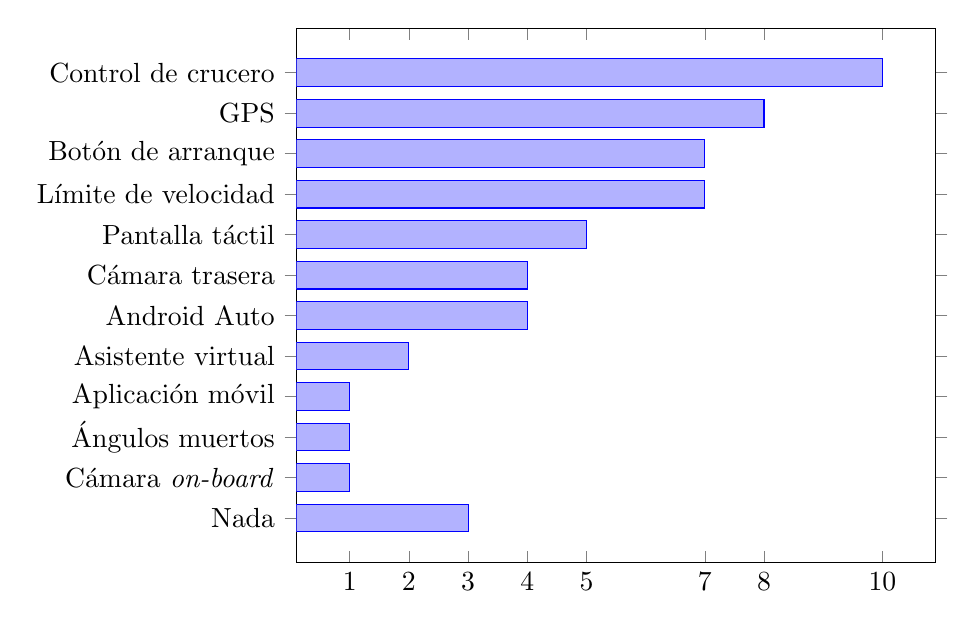
\begin{tikzpicture}
  \begin{axis} [%
      xbar,
      width=.8\linewidth,
      ytick=data,
      yticklabels={%
          Nada,
          Cámara \textit{on-board},
          Ángulos muertos,
          Aplicación móvil,
          Asistente virtual,
          Android Auto,
          Cámara trasera,
          Pantalla táctil,
          Límite de velocidad,
          Botón de arranque,
          GPS,
          Control de crucero,
        },
      xtick=data,
    ]
    \addplot coordinates {
        (3, 0)
        (1, 1)
        (1, 2)
        (1, 3)
        (2, 4)
        (4, 5)
        (4, 6)
        (5, 7)
        (7, 8)
        (7, 9)
        (8, 10)
        (10, 11)
      };
  \end{axis}
\end{tikzpicture}

\section{Estudio matemático}\label{sec:maths}
El estudio matemático va muy ligado al punto anterior (\ref{sec:merch}) ya que se
analizan los parámetros de \ac{OBD}--II y su ecuación matemática para obtener un
valor en $\mathbb{R}$ entendible por las personas.

Antes de dar paso a las ecuaciones en sí, es importante entender cómo funciona
el conector \ac{OBD}--II en esta situación. Los datos enviados y recibidos por
el coche están siempre codificados en un valor binario, recogido en un vector
de cuatro elementos en donde cada elemento tiene un \textit{byte} de tamaño. De
esta forma, se define al valor obtenido tras leer el conector \ac{OBD}--II como:

\begin{table}[H]
  \centering
  \resizebox{\textwidth}{!}{\begin{tabular}{|c|c|c|c|c|c|c|c|c|c|c|c|c|c|c|c|c|c|c|c|c|c|c|c|c|c|c|c|c|c|c|c|}
      \hline
      \multicolumn{8}{|c|}{$A$} & \multicolumn{8}{|c|}{$B$} & \multicolumn{8}{|c|}{$C$} & \multicolumn{8}{|c|}{$D$}                                                                                                                                                                                                                                 \\
      \hline
      $A_7$                     & $A_6$                     & $A_5$                     & $A_4$                     & $A_3$ & $A_2$ & $A_1$ & $A_0$ & $B_7$ & $B_6$ & $B_5$ & $B_4$ & $B_3$ & $B_2$ & $B_1$ & $B_0$ & $C_7$ & $C_6$ & $C_5$ & $C_4$ & $C_3$ & $C_2$ & $C_1$ & $C_0$ & $D_7$ & $D_6$ & $D_5$ & $D_4$ & $D_3$ & $D_2$ & $D_1$ & $D_0$ \\
      \hline
    \end{tabular}}
  \caption{Vector de \textit{bytes} que representa los datos recibidos del conector \ac{OBD}--II \cite{OBDIIPIDs2021}.}
  \label{tab:byte-array}
\end{table}

De esta forma, cuando se escribe $A_4$ se hace referencia al cuarto bit
del vector $A$. Los bits están ordenados según \ac{MSB}, de forma que
$A_7$ es el bit más significativo y $A_0$ el menor.

Los datos se obtienen del \ac{OBD}--II utilizando un lenguaje estándar llamado
\ac{PID}. El \ac{PID} se codifica como un número entero de 16 bits en donde los 8
primeros bits identifican el servicio/modo y los 8 restantes la operación a realizar.
Actualmente, están registrados los siguientes modos de funcionamiento (tabla
\ref{tab:pids-mode}):

\begin{table}[H]
  \centering
  \begin{tabularx}{\textwidth}{ | c | X | }
    \hline
    \textbf{Modo (hex)} & \textbf{Descripción}                                                                       \\
    \hline
    \texttt{01}         & Muestra los datos actuales del vehículo                                                    \\
    \hline
    \texttt{02}         & Muestra los datos almacenados del cuadro del vehículo                                      \\
    \hline
    \texttt{03}         & Muestra los códigos \ac{DTC}                                                               \\
    \hline
    \texttt{04}         & Elimina los códigos \ac{DTC} almacenados                                                   \\
    \hline
    \texttt{05}         & Resultados del test del sensor de oxígeno (sin \ac{CAN})                                   \\
    \hline
    \texttt{06}         & Resultados del test del sensor de oxígeno (con \ac{CAN})                                   \\
    \hline
    \texttt{07}         & Muestra los códigos \ac{DTC} pendientes (eliminados durante el último ciclo de conducción) \\
    \hline
    \texttt{08}         & Operaciones de control sobre los componentes del sistema                                   \\
    \hline
    \texttt{09}         & Petición de información sobre el vehículo                                                  \\
    \hline
    \texttt{0A}         & Códigos \ac{DTC} eliminados                                                                \\
    \hline
  \end{tabularx}
  \caption{Lista de modos de funcionamiento del estándar \ac{OBD}--II \cite{OBDIIPIDs2021}.}
  \label{tab:pids-mode}
\end{table}

Es importante destacar que no todos los fabricantes tienen por qué soportar todos
los modos, y que además ciertos fabricantes pueden definir sus modos propios por encima
del valor \texttt{09}.

Todos los modos definidos anteriormente tienen un conjunto de órdenes de soporte
en donde el sistema indica qué \ac{PID}s están soportados y cuáles no, por cada 32
\ac{PID}s. Por ejemplo, enviar la orden \texttt{0x0100} (\textit{modo 1, PID 0})
devolverá un valor que representará si los siguientes 32 \ac{PID}s están soportados.
Si el valor fuese, por ejemplo, \texttt{BE1FA813} se tendría que:

\begin{table}[H]
  \centering
  \resizebox{\textwidth}{!}{\begin{tabular}{ | c | c | c | c | c | c | c | c | c | c | c | c | c | c | c | c | c | c | c | c | c | c | c | c | c | c | c | c | c | c | c | c | c | }
      \hline
      \textbf{Hexadecimal} & \multicolumn{4}{|c|}{\texttt{B}} & \multicolumn{4}{|c|}{\texttt{E}} & \multicolumn{4}{|c|}{\texttt{1}} & \multicolumn{4}{|c|}{\texttt{F}} & \multicolumn{4}{|c|}{\texttt{A}} & \multicolumn{4}{|c|}{\texttt{8}} & \multicolumn{4}{|c|}{\texttt{1}} & \multicolumn{4}{|c|}{\texttt{3}}                                                                                                                                                                                                                                                                                                                                                 \\
      \hline
      \textbf{Binario}     & \texttt{1}                       & \texttt{0}                       & \texttt{1}                       & \texttt{1}                       & \texttt{1}                       & \texttt{1}                       & \texttt{1}                       & \texttt{0}                       & \texttt{0}  & \texttt{0}  & \texttt{0}  & \texttt{1}  & \texttt{1}  & \texttt{1}  & \texttt{1}  & \texttt{1}  & \texttt{1}  & \texttt{0}  & \texttt{1}  & \texttt{0}  & \texttt{1}  & \texttt{0}  & \texttt{0}  & \texttt{0}  & \texttt{0}  & \texttt{0}  & \texttt{0}  & \texttt{1}  & \texttt{0}  & \texttt{0}  & \texttt{1}  & \texttt{1}  \\
      \hline
      \textbf{?`Soportado?} & \done                            & \wontfix                         & \done                            & \done                            & \done                            & \done                            & \done                            & \wontfix                         & \wontfix    & \wontfix    & \wontfix    & \done       & \done       & \done       & \done       & \done       & \done       & \wontfix    & \done       & \wontfix    & \done       & \wontfix    & \wontfix    & \wontfix    & \wontfix    & \wontfix    & \wontfix    & \done       & \wontfix    & \wontfix    & \done       & \done       \\
      \hline
      \textbf{PID}         & \texttt{01}                      & \texttt{02}                      & \texttt{03}                      & \texttt{04}                      & \texttt{05}                      & \texttt{06}                      & \texttt{07}                      & \texttt{08}                      & \texttt{09} & \texttt{0A} & \texttt{0B} & \texttt{0C} & \texttt{0D} & \texttt{0E} & \texttt{0F} & \texttt{10} & \texttt{11} & \texttt{12} & \texttt{13} & \texttt{14} & \texttt{15} & \texttt{16} & \texttt{17} & \texttt{18} & \texttt{19} & \texttt{1A} & \texttt{1B} & \texttt{1C} & \texttt{1D} & \texttt{1E} & \texttt{1F} & \texttt{20} \\
      \hline
    \end{tabular}}
  \caption{Obtención de los \ac{PID}s soportados según el modo \cite{OBDIIPIDs2021}.}
  \label{tab:supported-pids}
\end{table}

A continuación, se dejan un conjunto de \ac{PID}s que se van a implementar en el
proyecto así como el código de acceso a ellos y la ecuación que permite obtener el
valor real.

\subsection*{Modo \texttt{01}}
Este modo permite acceder a la información en tiempo real del vehículo, según se
está en marcha. Los datos a los que se accede son:

\begin{table}[H]
  \centering
  \begin{tabularx}{\textwidth}{|c|X|}
    \hline
    \textbf{PID (hex)}       & \texttt{04}                    \\
    \hline
    \textbf{Bytes devueltos} & $1$                            \\
    \hline
    \textbf{Descripción}     & Carga del motor, en porcentaje \\
    \hline
    \textbf{Valor mínimo}    & $0\%$                          \\
    \hline
    \textbf{Valor máximo}    & $100\%$                        \\
    \hline
    \textbf{Fórmula}         &                                %
    \begin{equation*}
      \frac{A}{2.55}
    \end{equation*}                                 \\
    \hline
  \end{tabularx}
  \caption{\ac{PID} \texttt{04} -- carga del motor, en $\%$.}
\end{table}

\begin{table}[H]
  \centering
  \begin{tabularx}{\textwidth}{|c|X|}
    \hline
    \textbf{PID (hex)}       & \texttt{05}                            \\
    \hline
    \textbf{Bytes devueltos} & $1$                                    \\
    \hline
    \textbf{Descripción}     & Temperatura del refrigerante del motor \\
    \hline
    \textbf{Valor mínimo}    & $-40~\tccentigrade$                    \\
    \hline
    \textbf{Valor máximo}    & $215~\tccentigrade$                    \\
    \hline
    \textbf{Fórmula}         &                                        %
    \begin{equation*}
      A - 40
    \end{equation*}                                         \\
    \hline
  \end{tabularx}
  \caption{\ac{PID} \texttt{05} -- temperatura del refrigerante del motor, en $\tccentigrade$.}
\end{table}

\begin{table}[H]
  \centering
  \begin{tabularx}{\textwidth}{|c|X|}
    \hline
    \textbf{PID (hex)}       & \texttt{0C}         \\
    \hline
    \textbf{Bytes devueltos} & $2$                 \\
    \hline
    \textbf{Descripción}     & Velocidad del motor \\
    \hline
    \textbf{Valor mínimo}    & $0~RPM$             \\
    \hline
    \textbf{Valor máximo}    & $16383.75~RPM$      \\
    \hline
    \textbf{Fórmula}         &                     %
    \begin{equation*}
      \frac{256A + B}{4}
    \end{equation*}                      \\
    \hline
  \end{tabularx}
  \caption{\ac{PID} \texttt{0C} -- velocidad del motor, en $RPM$.}
\end{table}

\begin{table}[H]
  \centering
  \begin{tabularx}{\textwidth}{|c|X|}
    \hline
    \textbf{PID (hex)}       & \texttt{0D}            \\
    \hline
    \textbf{Bytes devueltos} & $1$                    \\
    \hline
    \textbf{Descripción}     & Velocidad del vehículo \\
    \hline
    \textbf{Valor mínimo}    & $0~\nicefrac{km}{h}$   \\
    \hline
    \textbf{Valor máximo}    & $255~\nicefrac{km}{h}$ \\
    \hline
    \textbf{Fórmula}         &                        %
    \begin{equation*}
      A
    \end{equation*}                         \\
    \hline
  \end{tabularx}
  \caption{\ac{PID} \texttt{0D} -- velocidad del vehículo, en $\nicefrac{km}{h}$.}
\end{table}

\begin{table}[H]
  \centering
  \begin{tabularx}{\textwidth}{|c|X|}
    \hline
    \textbf{PID (hex)}       & \texttt{11}             \\
    \hline
    \textbf{Bytes devueltos} & $1$                     \\
    \hline
    \textbf{Descripción}     & Posición del acelerador \\
    \hline
    \textbf{Valor mínimo}    & $0\%$                   \\
    \hline
    \textbf{Valor máximo}    & $100\%$                 \\
    \hline
    \textbf{Fórmula}         &                         %
    \begin{equation*}
      \frac{A}{2.55}
    \end{equation*}                          \\
    \hline
  \end{tabularx}
  \caption{\ac{PID} \texttt{11} -- posición del acelerador, en $\%$.}
\end{table}

\begin{table}[H]
  \centering
  \begin{tabularx}{\textwidth}{|c|X|}
    \hline
    \textbf{PID (hex)}       & \texttt{2F}                      \\
    \hline
    \textbf{Bytes devueltos} & $1$                              \\
    \hline
    \textbf{Descripción}     & Nivel del tanque del combustible \\
    \hline
    \textbf{Valor mínimo}    & $0\%$                            \\
    \hline
    \textbf{Valor máximo}    & $100\%$                          \\
    \hline
    \textbf{Fórmula}         &                                  %
    \begin{equation*}
      \frac{A}{2.55}
    \end{equation*}                                   \\
    \hline
  \end{tabularx}
  \caption{\ac{PID} \texttt{2F} -- nivel del tanque del combustible, en $\%$.}
\end{table}

\begin{table}[H]
  \centering
  \begin{tabularx}{\textwidth}{|c|X|}
    \hline
    \textbf{PID (hex)}       & \texttt{46}          \\
    \hline
    \textbf{Bytes devueltos} & $1$                  \\
    \hline
    \textbf{Descripción}     & Temperatura ambiente \\
    \hline
    \textbf{Valor mínimo}    & $-40~\tccentigrade$  \\
    \hline
    \textbf{Valor máximo}    & $215~\tccentigrade$  \\
    \hline
    \textbf{Fórmula}         &                      %
    \begin{equation*}
      A - 40
    \end{equation*}                      \\
    \hline
  \end{tabularx}
  \caption{\ac{PID} \texttt{46} -- temperatura ambiente, en $\tccentigrade$.}
\end{table}

\begin{table}[H]
  \centering
  \begin{tabularx}{\textwidth}{|c|X|}
    \hline
    \textbf{PID (hex)}       & \texttt{5B}                           \\
    \hline
    \textbf{Bytes devueltos} & $1$                                   \\
    \hline
    \textbf{Descripción}     & Tiempo restante de la batería híbrida \\
    \hline
    \textbf{Valor mínimo}    & $0\%$                                 \\
    \hline
    \textbf{Valor máximo}    & $100\%$                               \\
    \hline
    \textbf{Fórmula}         &                                       %
    \begin{equation*}
      \frac{A}{2.55}
    \end{equation*}                                       \\
    \hline
  \end{tabularx}
  \caption{\ac{PID} \texttt{5B} -- tiempo restante de la batería híbrida, en $\%$.}
\end{table}

\begin{table}[H]
  \centering
  \begin{tabularx}{\textwidth}{|c|X|}
    \hline
    \textbf{PID (hex)}       & \texttt{5C}            \\
    \hline
    \textbf{Bytes devueltos} & $1$                    \\
    \hline
    \textbf{Descripción}     & Temperatura del aceite \\
    \hline
    \textbf{Valor mínimo}    & $-40~\tccentigrade$    \\
    \hline
    \textbf{Valor máximo}    & $215~\tccentigrade$    \\
    \hline
    \textbf{Fórmula}         &                        %
    \begin{equation*}
      A - 40
    \end{equation*}                        \\
    \hline
  \end{tabularx}
  \caption{\ac{PID} \texttt{5C} -- temperatura del aceite, en $\tccentigrade$.}
\end{table}

\begin{table}[H]
  \centering
  \begin{tabularx}{\textwidth}{|c|X|}
    \hline
    \textbf{PID (hex)}       & \texttt{5E}               \\
    \hline
    \textbf{Bytes devueltos} & $2$                       \\
    \hline
    \textbf{Descripción}     & Consumo actual del motor  \\
    \hline
    \textbf{Valor mínimo}    & $0~\nicefrac{l}{h}$       \\
    \hline
    \textbf{Valor máximo}    & $3212.75~\nicefrac{l}{h}$ \\
    \hline
    \textbf{Fórmula}         &                           %
    \begin{equation*}
      \frac{256A + B}{20}
    \end{equation*}                           \\
    \hline
  \end{tabularx}
  \caption{\ac{PID} \texttt{5E} -- consumo actual del motor, en $\nicefrac{L}{h}$.}
\end{table}

\begin{table}[H]
  \centering
  \begin{tabularx}{\textwidth}{|c|X|}
    \hline
    \textbf{PID (hex)}       & \texttt{61}                       \\
    \hline
    \textbf{Bytes devueltos} & $1$                               \\
    \hline
    \textbf{Descripción}     & Torque demandado por el conductor \\
    \hline
    \textbf{Valor mínimo}    & $-125\%$                          \\
    \hline
    \textbf{Valor máximo}    & $130\%$                           \\
    \hline
    \textbf{Fórmula}         &                                   %
    \begin{equation*}
      A - 125
    \end{equation*}                                   \\
    \hline
  \end{tabularx}
  \caption{\ac{PID} \texttt{61} -- torque demandado por el conductor, en $\%$.}
\end{table}

\begin{table}[H]
  \centering
  \begin{tabularx}{\textwidth}{|c|X|}
    \hline
    \textbf{PID (hex)}       & \texttt{62}             \\
    \hline
    \textbf{Bytes devueltos} & $1$                     \\
    \hline
    \textbf{Descripción}     & Torque actual del motor \\
    \hline
    \textbf{Valor mínimo}    & $-125\%$                \\
    \hline
    \textbf{Valor máximo}    & $130\%$                 \\
    \hline
    \textbf{Fórmula}         &                         %
    \begin{equation*}
      A - 125
    \end{equation*}                         \\
    \hline
  \end{tabularx}
  \caption{\ac{PID} \texttt{62} -- torque actual del motor, en $\%$.}
\end{table}

\begin{table}[H]
  \centering
  \begin{tabularx}{\textwidth}{|c|X|}
    \hline
    \textbf{PID (hex)}       & \texttt{63}                    \\
    \hline
    \textbf{Bytes devueltos} & $2$                            \\
    \hline
    \textbf{Descripción}     & Torque de referencia del motor \\
    \hline
    \textbf{Valor mínimo}    & $0~Nm$                  \\
    \hline
    \textbf{Valor máximo}    & $65535~Nm$              \\
    \hline
    \textbf{Fórmula}         &                                %
    \begin{equation*}
      256A + B
    \end{equation*}                                \\
    \hline
  \end{tabularx}
  \caption{\ac{PID} \texttt{63} -- torque de referencia del motor, en $Nm$.}
\end{table}

\begin{table}[H]
  \centering
  \begin{tabularx}{\textwidth}{|c|X|}
    \hline
    \textbf{PID (hex)}       & \texttt{A4}                \\
    \hline
    \textbf{Bytes devueltos} & $4$                        \\
    \hline
    \textbf{Descripción}     & Marcha actual del vehículo \\
    \hline
    \textbf{Valor mínimo}    & $0~\text{ratio}$           \\
    \hline
    \textbf{Valor máximo}    & $65535~\text{ratio}$       \\
    \hline
    \textbf{Fórmula}         &                            %
    \begin{equation*}
      \begin{aligned}
        A_1 & = 1 \Longrightarrow \text{soportado} \\
        R   & = \frac{256C + D}{1000}
      \end{aligned}
    \end{equation*}                            \\
    \hline
  \end{tabularx}
  \caption{\ac{PID} \texttt{A4} -- marcha actual del vehículo, en ratio.}
\end{table}

\begin{table}[H]
  \centering
  \begin{tabularx}{\textwidth}{|c|X|}
    \hline
    \textbf{PID (hex)}       & \texttt{A6}      \\
    \hline
    \textbf{Bytes devueltos} & $4$              \\
    \hline
    \textbf{Descripción}     & Odómetro         \\
    \hline
    \textbf{Valor mínimo}    & $0~km$           \\
    \hline
    \textbf{Valor máximo}    & $429496729.5~km$ \\
    \hline
    \textbf{Fórmula}         &                  %
    \begin{equation*}
      \frac{A\left(2^{24}\right) + B\left(2^{16}\right) + C\left(2^8\right) + D}{10}
    \end{equation*}                  \\
    \hline
  \end{tabularx}
  \caption{\ac{PID} \texttt{A6} -- odómetro, en $km$.}
\end{table}

\subsection*{Modo \texttt{03}}
El modo \texttt{03} devuelve los \ac{DTC} guardados de la sesión actual. Estos códigos
de diagnóstico representan los distintos errores que hay en el vehículo, con un conjunto
de bytes que los identifican.

Este modo, a diferencia de los otros, no requiere de un parámetro \ac{PID} sino que solo
se envía el servicio como identificador. Una petición al modo \texttt{03} devolverá una
lista de $n$ elementos en donde cada elemento ocupa 2 bytes (por ende, el tamaño
esperable de la trama es $2n$).

Los códigos de error se definen como un conjunto de 5 caracteres de la forma: ``\texttt{U0158}''.
El valor de los caracteres define así:

\begin{table}[H]
  \centering
  \begin{minipage}{.32\linewidth}
    \begin{tabularx}{\textwidth}{|C{.3}|C{.7}|}
      \hline
      $A_7$ - $A_6$ & \textbf{Primer caracter \ac{DTC}}                         \\
      \hline
      \texttt{00}             & \textbf{P} -- sistema de propulsión (\textit{powertrain}) \\
      \texttt{01}             & \textbf{C} -- chassis                                     \\
      \texttt{10}             & \textbf{B} -- cuerpo (\textit{body})                      \\
      \texttt{11}             & \textbf{U} -- comunicaciones (\textit{network})           \\
      \hline
    \end{tabularx}
  \end{minipage}
  \hfill
  \begin{minipage}{.32\linewidth}
    \begin{tabularx}{\textwidth}{|C{.3}|C{.7}|}
      \hline
      $A_5$ - $A_4$ & \textbf{Segundo caracter \ac{DTC}} \\
      \hline
      \texttt{00}             & \texttt{0}                         \\
      \texttt{01}             & \texttt{1}                         \\
      \texttt{10}             & \texttt{2}                         \\
      \texttt{11}             & \texttt{3}                         \\
      \hline
    \end{tabularx}
  \end{minipage}
  \hfill
  \begin{minipage}{.32\linewidth}
    \begin{tabularx}{\textwidth}{|C{.3}|C{.7}|}
      \hline
      $A_3$ - $A_0$ & \textbf{Tercer caracter \ac{DTC}} \\
      \hline
      \texttt{0000}             & \texttt{0}                        \\
      \texttt{0001}             & \texttt{1}                        \\
      \texttt{0010}             & \texttt{2}                        \\
      \texttt{0011}             & \texttt{3}                        \\
      \texttt{0100}             & \texttt{4}                        \\
      \texttt{0101}             & \texttt{5}                        \\
      \texttt{0110}             & \texttt{6}                        \\
      \texttt{0111}             & \texttt{7}                        \\
      \texttt{1000}             & \texttt{8}                        \\
      \texttt{1001}             & \texttt{9}                        \\
      \texttt{1010}             & \texttt{A}                        \\
      \texttt{1011}             & \texttt{B}                        \\
      \texttt{1100}             & \texttt{C}                        \\
      \texttt{1101}             & \texttt{D}                        \\
      \texttt{1110}             & \texttt{E}                        \\
      \texttt{1111}             & \texttt{F}                        \\
      \hline
    \end{tabularx}
  \end{minipage}
\end{table}

Los caracteres cuarto y quinto se corresponden a los bits $B_7$ -- $B_4$ y $B_3$ -- $B_0$
respectivamente, y siguen la notación hexadecimal (al igual que los bits $A_3$ -- $A_0$).

De esta forma, con el código ya extraído, se necesita mirar en una tabla de valores
\ac{DTC} para saber exactamente a qué error se corresponde. Una web muy interesante
es la de ``OBD-Codes.com'' \cite{OBDCodesComLeading}, en donde hay información tanto
de códigos \ac{DTC} estándar como de códigos propietarios. Mirando en la propia
web, el código \texttt{U0158} se correspondería a: ``\textit{Lost communication with
head-up display}''\footnote{En la propia web dan muchos detalles e información
extendida sobre el error en cuestión, al igual que procedimientos para poder
solucionar el problema -- \url{https://www.obd-codes.com/u0158}}.

\subsection*{Modo \texttt{09}}
El modo \texttt{09} devuelve información referente al vehículo en sí, no al estado
de los sensores o del propio vehículo. Algunos datos interesantes son:

\begin{table}[H]
  \centering
  \begin{tabularx}{\textwidth}{|c|X|}
    \hline
    \textbf{PID (hex)}       & \texttt{02}                    \\
    \hline
    \textbf{Bytes devueltos} & $17$                            \\
    \hline
    \textbf{Descripción}     & \ac{VIN} \\
    \hline
    \textbf{Fórmula}         & \ac{VIN} de 17 caracteres ASCII con \textit{padding} a la izquierda de caracteres nulos (\texttt{0x00}) si hace falta \\
    \hline
  \end{tabularx}
  \caption{\ac{PID} \texttt{02} -- \ac{VIN}.}
\end{table}

\begin{table}[H]
  \centering
  \begin{tabularx}{\textwidth}{|c|X|}
    \hline
    \textbf{PID (hex)}       & \texttt{0A}                    \\
    \hline
    \textbf{Bytes devueltos} & $20$                            \\
    \hline
    \textbf{Descripción}     & Nombre de la \ac{ECU} \\
    \hline
    \textbf{Fórmula}         & 20 caracteres ASCII con \textit{padding} a la derecha de caracteres nulos (\texttt{0x00}) \\
    \hline
  \end{tabularx}
  \caption{\ac{PID} \texttt{0A} -- nombre de la \ac{ECU}.}
\end{table}

\section{Diseño \textit{software}}\label{sec:software}
El proyecto cuenta con una parte \textit{software} muy importante, ya que está
conformado por múltiples sistemas que deben cooperar entre sí. Por una parte,
el desarrollo del \textit{software} del proyecto aborda los siguientes aspectos:

\begin{itemize}
  \item Desarrollo de la aplicación embebida que irá en el dispositivo enganchado
        al coche en sí. En dicho dispositivo se programará, entre otros, la planificación
        del sistema según el análisis de planificabilidad llevado a cabo en el punto
        \ref{sec:rt-design}, la gestión de los datos y de la información y la transmisión
        al servidor remoto.
  \item Desarrollo de la infraestructura en la nube que alojará la lógica de almacenamiento de
        los datos y de la información generada a partir de ellos para los usuarios de
        dispositivos \ac{VIMS}.
  \item Desarrollo de la aplicación web que servirá de pasarela entre los usuarios
        y sus datos alojados en el servidor en la nube, mediante una interfaz de usuario
        que facilitará ciertas tareas de gestión y la observación de los datos.
  \item Desarrollo de la aplicación móvil que permitirá la conexión directa con la
        placa \ac{VIMS} para su configuración inicial y la visualización de la información
        en el momento.
\end{itemize}

El sistema sigue el prototipo de una arquitectura cliente--servidor, con uno o varios
clientes que se conectan a un servidor en la nube que realiza tareas de gestión de
la información, entre otros.

Uno de los requisitos principales de la aplicación (que se vio además en el estudio
del mercado) era que esta fuese accesible, simple y fácil de entender. Mediante la
definición de tanto la aplicación web como la aplicación móvil se pretende unificar
el acceso a la información de los usuarios y sus vehículos. Con ambas aplicaciones,
se busca que de un vistazo se tenga acceso a los últimos viajes, estadísticas,
perfiles de conducción y demás.

Además, la arquitectura del servidor permite generar notificaciones personalizadas
cuando sucedan ciertos eventos. Por ejemplo, se pueden enviar correos electrónicos
con información sobre el último viaje, cuánto ha durado el depósito de gasolina, fecha
recomendada para el siguiente mantenimiento, revisión del estado de los neumáticos,
etc. De esta manera, se pretende que el usuario no esté directamente pendiente del
estado mecánico de su vehículo sino que delegue esa tarea en el sistema \ac{VIMS}.

Por su lado, la programación del dispositivo \ac{VIMS} en sí es una parte crítica y
fundamental en el desarrollo del proyecto. El dispositivo va a estar en un entorno
no controlado con condiciones cambiantes, sobre todo en lo referente a las comunicaciones.
Es fundamental que el desarrollo del \textit{software} del dispositivo embebido
sea resiliente y esté diseñado para soportar situaciones adversas en lo referente
a la transmisión de la información.

Esto se detalla más adelante en los requisitos, y algunas de las características que
se necesitan tener en el dispositivo en sí son el almacenamiento provisional de los
datos, la retransmisión de la información en caso de fallo, modos de bajo consumo
cuando el vehículo no está en marcha, etc.

\section{Diseño \textit{hardware}}\label{sec:hardware}
Los elementos \textit{hardware} hacen referencia directa al dispositivo \ac{VIMS}
que irá embebido en el vehículo y al resto de componentes que son necesarios para
un correcto funcionamiento del mismo. En esta sección también se incluye el
diseño 3D de la caja contenedora del dispositivo.

En términos generales, el \textit{hardware} en que se descompone el proyecto es:

\begin{itemize}
  \item Dispositivo controlador \ac{SoC} ESP32, que incluye de fábrica radios WiFi y Bluetooth.
  \item Dispositivo de control \ac{GPS}.
  \item Dispositivo de comunicaciones de red 4G.
  \item Dispositivo de almacenamiento de datos usando tarjetas microSD.
  \item Desarrollo de la placa de circuito impreso de control que engloba los elementos
        necesarios para el correcto desempeño del sistema.
  \item Diseño de la estructura 3D que albergará el dispositivo final y los componentes
        necesarios para su funcionamiento.
  \item Diseño de dispositivo que permita la adaptación del estándar \ac{OBD}--II a
        un protocolo entendible por el dispositivo embebido en sí, como el \ac{CAN}.
\end{itemize}

En primer lugar, se ha escogido ese \ac{SoC} por las características que
ofrece y el gran soporte (tanto oficial como de la comunidad) que tiene por detrás.
El \ac{SoC} cuenta con un microprocesador Xtensa LX6 de 32 bits con dos
núcleos que opera a 240 MHz. Además, cuenta con un co-procesador \ac{ULP} que permite realizar
ciertas operaciones con un consumo extremadamente bajo (del orden de los $\mu A$).

Además de lo anterior, tiene directamente integradas las antenas WiFi y Bluetooth
(estándares \texttt{802.11 b/g/n} y \texttt{v4.2 \ac{BR/EDR} + \ac{BLE}} respectivamente),
controlador \ac{PWM} integrado, controlador \ac{CAN} integrado, controlador para
tarjetas SD integrado, dos \ac{ADC} de 18 canales y 12 bits,
criptografía acelerada por \textit{hardware}, hasta 20 pines \ac{GPIO} y demás.

Junto con las características físicas anteriores, es importante destacar que el
ESP32 tiene soporte para ser programado usando el \textit{framework} de Arduino.
Esto facilita la labor de programación y evita tener que entrar
en excesivo detalle sobre cómo se puede configurar la placa internamente
(por ejemplo, ajuste de registros, esperar a la carga de los condensadores, \dots)
pero abriendo la posibilidad a ello si hace falta. Además, el \ac{SoC} tiene
soporte nativo para FreeRTOS, que será lo que se use para programar las tareas
en tiempo real del controlador.

Por otra parte, el resto de conectores que se necesitan en el dispositivo son muy
variados y cada uno tiene sus particularidades. Es por esto que se ha decidido
buscar una PCB que ya aunase la lógica de diseño necesaria para que el \ac{SoC}
tenga soporte para ellos. Se realizó una exploración sobre las
distintas alternativas existentes y finalmente se tomó la decisión de usar la
placa LILYGO TTGO T-SIM7000G (figura \ref{fig:lilygo}) que tiene soporte nativo
para tarjeta SIM con conexión \ac{LTE}, antena \ac{GPS}, tarjeta microSD, batería
externa y carga solar.

\begin{figure}[H]
  \centering
  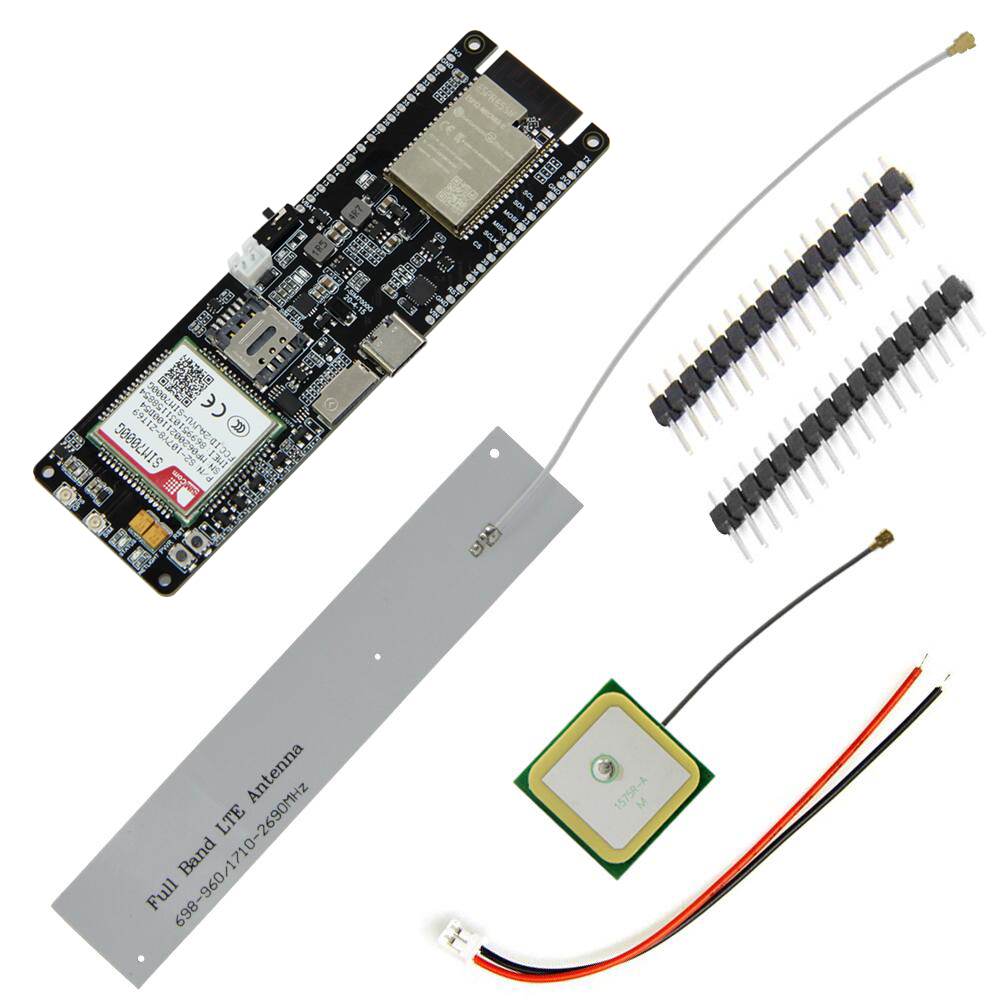
\includegraphics[width=\linewidth]{images/lilygo-tsim7000g.jpg}
  \caption{Placa de desarrollo LILYGO TTGO T-SIM7000G usada en el proyecto \cite{4269LILYGO}.}
  \label{fig:lilygo}
\end{figure}

En lo referente al conexionado con el coche, y en estrecha relación con el diseño 3D,
se buscó un conector hembra de \ac{OBD}--II que permitiese definir el \textit{pinout}
hacia la placa en este caso. Se valoraron distintas opciones, y una de las más
interesantes resultó la siguiente:

\begin{figure}[H]
  \centering
  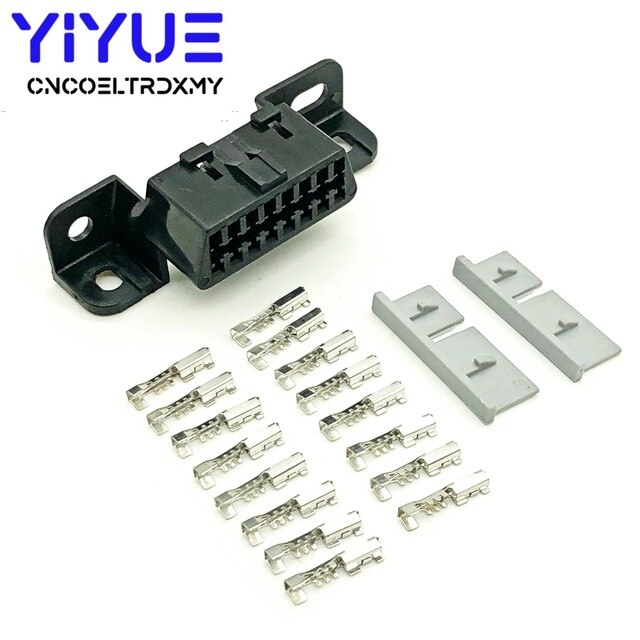
\includegraphics[width=\linewidth]{images/obd2-female.jpeg}
  \caption{Conector \ac{OBD}--II hembra con posibilidad de definir los pines de salida \cite{10DESCUENTOConector}.}
\end{figure}

También existen otros modelos que vienen ya configurados y que son más simples de
implementar, como:

\begin{figure}[H]
  \centering
  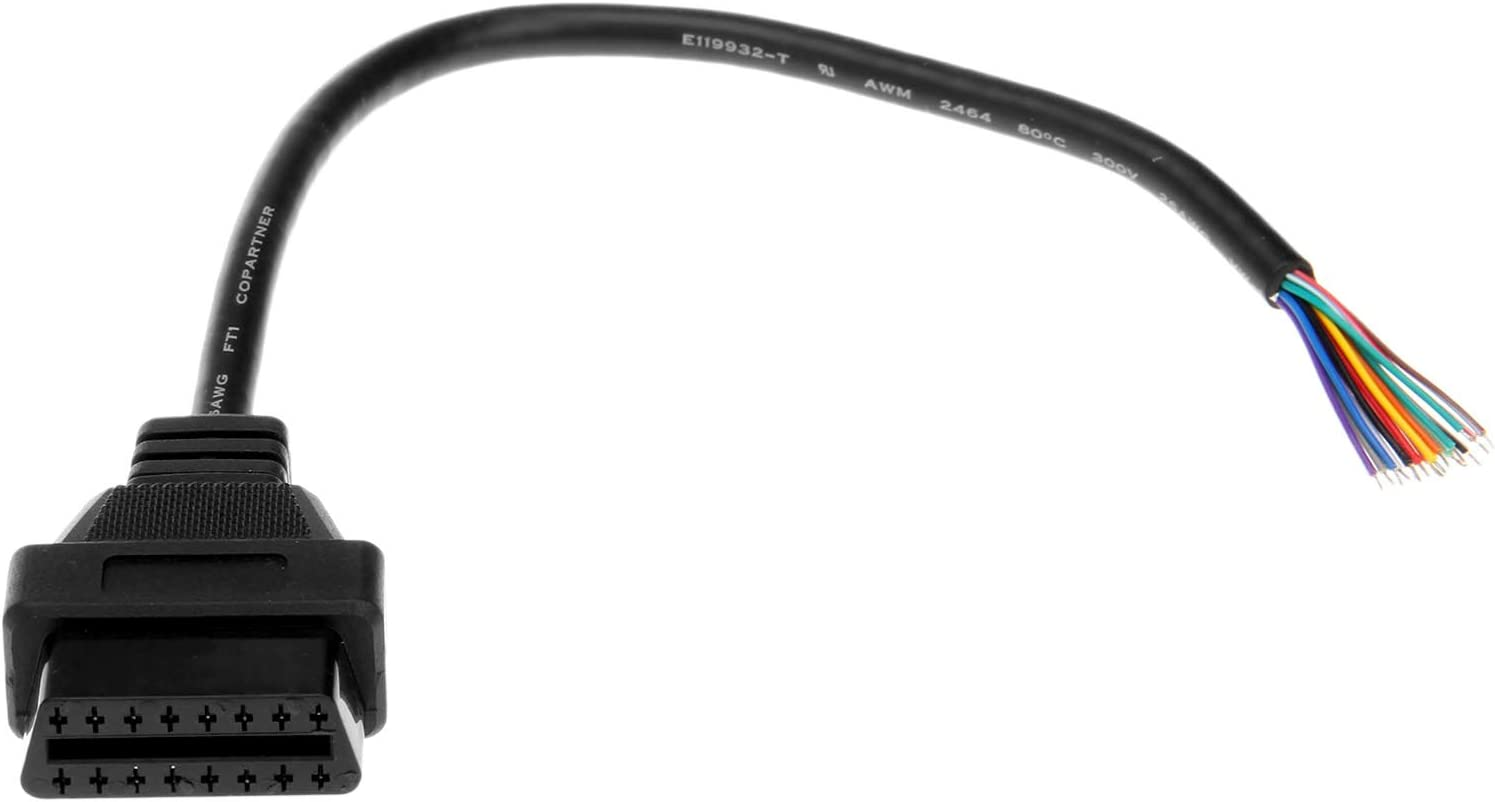
\includegraphics[width=\linewidth]{images/obd2-female-amazon.jpg}
  \caption{Conector \ac{OBD}--II hembra con cables ya incluidos \cite{AmazonComAupoko}.}
\end{figure}

Finalmente, para gestionar los sensores y conectores que necesita tener la placa para
funcionar correctamente, se diseñará una PCB que definirá la lógica de conexionado
para el correcto funcionamiento de todo el sistema al conjunto.

\section{Análisis de planificabilidad}\label{sec:rt-analysis}
A raíz del apartado anterior y de la cantidad de datos que se pretenden recoger
durante el funcionamiento del sistema, una parte fundamental es la planificación
de las tareas del mismo.

En principio, \ac{VIMS} no se define como un sistema en tiempo real. Sin embargo,
la envergadura del proyecto y la cantidad de acciones a realizar de forma coordinada
y concurrente requiere de una planificación del proyecto a la hora de definir tareas,
plazos y periodos.

En un primer análisis, se detectan las siguientes casuísticas que llevarán asociada
la tarea pertinente:

\begin{enumerate}
  \item Lectura de datos desde el conector \ac{OBD}--II. Esta tarea almacenará la
        información en crudo del conector en una estructura de datos propia, preparada
        para que otra tarea los adapte y transforme en información entendible. Además,
        establecerá una marca temporal para los datos de manera que se sepa exactamente
        en qué momento se obtuvieron.
  \item Conversión de los datos leídos desde el \ac{OBD}--II. Esta tarea deberá
        leer y convertir los datos almacenados en crudo por el \ac{OBD}--II en
        datos legibles y entendibles por el ser humando. Se encargará además de
        definir las unidades de medida asociadas al dato en sí.
  \item Transmisión de los datos al servidor en la nube. Esta tarea deberá enviar
        los datos ya preparados con su unidad correspondiente y su marca temporal
        usando el protocolo MQTT al servidor en la nube. Según la tecnología de
        recepción presente en el \textit{backend}, se pueden enviar los datos
        individualmente a un \textit{endpoint} específico de MQTT (lo cual simplificaría
        la gestión de la información por parte del servidor) o se deberán enviar todos
        en conjunto como un JSON al servidor en backend.
  \item Persistencia de los datos en la tarjeta microSD. Esta tarea almacenará
        los datos provisionalmente en la tarjeta microSD si no han podido ser enviados
        al servidor remoto (por ejemplo, por no disponibilidad de la red). Se deberán
        serializar los datos junto con su marca temporal para una posterior retransmisión
        cuando haya disponibilidad de red.
  \item Estado de la conectividad de red. Esta tarea se encargará de comprobar
        periódicamente que la conexión de red está disponible y es accesible desde
        el dispositivo, simplificando la lógica de comunicación del resto de tareas.
  \item Sincronización del reloj con la red. Esta tarea se encargará, mediante el
        protocolo \ac{NTP}, de mantener el reloj interno de la placa sincronizado con el
        tiempo \ac{UTC}, de forma que todas las marcas temporales asociadas están siempre
        con la hora adecuada.
  \item Ubicación del dispositivo. Esta tarea se encargará de actualizar la ubicación
        del dispositivo y almacenar los datos para su posterior envío al servidor remoto.
  \item Estado eléctrico del sistema. Esta tarea se encargará de comprobar periódicamente
        la tensión de entrada del sistema para detectar cambios drásticos en dicha
        tensión (de $\approx \pm 1.1V$) para saber cuándo el sistema debe entrar en
        modo de bajo consumo.
\end{enumerate}

Las tareas anteriores deberán planificarse siguiendo un esquema de planificación de
tiempo real que contemple frecuencia de activación, retardos relativos producidos
por la interdependencia de las tareas, tiempo de cómputo estimado, prioridades
según frecuencia, acceso a recursos compartidos y herencia de prioridad por acceso
a dichos recursos (prioridad de techo).


%% Requirements
\chapter{Especificación de requisitos}\label{chap:requirements}
%% Introduction
\begin{abstract}
  En este documento se va a tratar el diseño y especificación de \ac{VIMS},
  un proyecto de ingeniería que modela, diseña y arquitecta un sistema
  conformado por un dispositivo embebido y un servidor en la nube. El
  dispositivo se conecta al vehículo y transmite, mediante redes inalámbricas,
  los datos al servidor, que hará todo el procesamiento y gestión.
  El objetivo principal es devolverle al propietario del vehículo el control
  sobre el mismo, accediendo fácilmente a los datos recogidos por el automóvil
  así como de los mensajes de error.

  Para ello, primero se recogerán datos de una muestra de conductores y
  no conductores para identificar correctamente las necesidades de los
  usuarios y ajustar mejor el producto.
  
  A continuación, se elicitarán los requisitos que permitirán posteriormente
  modelar y diseñar el sistema de forma fiel. Esta fase permite trabajar
  directamente en los diagramas que modelan el sistema, tanto a nivel de
  casuísticas como en qué estructura deberá tener. Esto es fundamental porque
  simplificará y acotará las etapas de desarrollo posteriores.

  Además, se trabajará en el estudio del modelo matemático que permite traducir
  los datos recibidos por los vehículos según el estándar \ac{OBD}--II. A su vez,
  se estudiarán las características del sistema \textit{hardware} lo que permitirá
  desarrollar y construir una placa de control que será la encargada de gestionar los
  parámetros del dispositivo \ac{VIMS}.

  Por último, se estudian las distintas tareas en tiempo real que compondrán el sistema \ac{VIMS}
  mediante el análisis de tiempo de respuesta de las mismas. Dicho análisis
  determina la planificabilidad del sistema y asegura un correcto y predecible
  funcionamiento en cualquier circunstancia.
\end{abstract}

\selectlanguage{english}
\begin{abstract}
  \ac{VIMS} design and specification project is an integral engineering development
  which designs, models and architects a whole system built with an embedded
  device and a remote cloud server. The device is attached to the driver's vehicle
  and by using wireless communication transmits the data to the remote server,
  which handles the entire processing and data generation.
  The main objective is to bring the driver's sensation back of having control
  over the vehicle, easily accessing to the entire information it provides
  alongside error messages in an easy, accessible way.

  Firstly, a quest will be done so relevant data is collected from a sample
  of drivers and non-drivers which will help identifying their needs and
  better adjusting the final product.

  Then, the requirements will be elicited which will allow the modeling
  and the design of the system in further steps of the development.
  Such step allows working directly with the diagrams that will
  model the system in both behavioral and structural manners. This is
  crucial as it will simplify and delimit the next steps of the project.

  In addition, there will be a mathematical analysis on how to translate
  the data received from the vehicle itself into human-readable information,
  based on the \ac{OBD}--II standard. Furthermore, hardware characteristics
  will be studied which will allow developing and building a PCB which will
  handle the parameters of the \ac{VIMS} device.

  Finally, a real-time task analysis will be done for \ac{VIMS} system. This will lead us
  through the definition of the tasks themselves as well as the response time
  analysis for the whole system. Thus the analysis determines if the entire
  system can be scheduled asserting a well-known, correct behavior under any
  circumstances.
\end{abstract}

\selectlanguage{spanish}


\chapter{Introducción}\label{chap:intro}
En un mundo cada vez más interconectado, hay ciertas tecnologías que se quedan
por detrás en unos campos mientras que siguen progresando en otros. Esto se ve
directamente reflejado en la industria automovilística en donde los vehículos
cada vez cuentan con mayor y mejor tecnología (como cámaras, sensores, actuadores,
etc.) pero no es directamente accesible por el usuario: mediante pantallas e
interfaces se ofrecen métodos sencillos que facilitan su uso.

\ac{VIMS} pretende ser un sistema que facilite el acceso a todos los datos que
ofrece un vehículo para generar estadísticas, descubrir patrones en la conducción
y detectar errores. De esta forma, el conductor tendrá información de primera
mano sobre el estado de su vehículo, eficiencia de su conducción así como obtener
información en tiempo real complementaria a la ya propiciada por el vehículo.

\section{Estado del arte}\label{sec:state_of_the_art}
La historia de la automoción comienza estrictamente en el siglo XIX.
Un automóvil es, por definición, un vehículo que se mueve a sí mismo
(del griego, \textit{αὐτός} ``a sí mismo'' y del latín \textit{mobilis},
``que se mueve'').

Desde los primeros modelos como la serie T, de Ford, hasta el inicio de
la fabricación de vehículos por parte de Mercedes Benz, la historia del
automovilismo ha estado llena de grandes logros y avances en un intervalo
de tiempo relativamente pequeño (figura \ref{fig:ford_model_t}):

\begin{figure}[H]
  \centering
  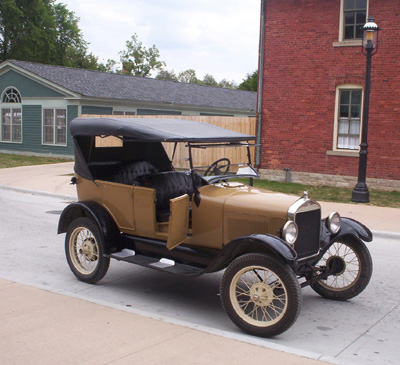
\includegraphics[width=.8\linewidth]{images/Late_model_Ford_Model_T.jpg}
  \caption{Ford modelo T del 1927 -- de Rmhermen \cite{Ford2022}.}
  \label{fig:ford_model_t}
\end{figure}

Durante aquella época, el ``mejor'' mecanismo de descubrimiento de
problemas era con algunos medidores y, sobre todo, por intuición:
sonidos del motor, olores extraños, \dots

No fue hasta los años 60 en donde los vehículos empezaron a incorporar
distintas interfaces con métricas que podían informar sobre el estado del
vehículo. El gran ``bum'' llegó con la expansión de la computadora, en donde
por primera vez se vio factible introducir un pequeño ordenador de 
abordo en el sistema.

En estos primeros sistemas, se incluyen indicadores del nivel de combustible,
sistema de refrigeración, presión del aceite, velocidad del motor,
temperatura del motor y otra información relativa al combustible. El
primer modelo que se conoce que incluye estos sistemas de cara a la
población en general es el Volkswagen Tipo III, en 1969 (figura \ref{fig:volkswagen_t3}):

\begin{figure}[H]
  \centering
  \includegraphics[width=.9\linewidth]{images/volkswagen_t3.jpg}
  \caption{Volkswagen Tipo III, modelo de inyección de 1969 -- de OSX - Trabajo propio \cite{VolkswagenTipo2021}.}
  \label{fig:volkswagen_t3}
\end{figure}

Pese a que supusieron un gran avance, estos primeros sistemas de
diagnóstico daban una información muy valiosa pero limitada, ya que muchos
diagnósticos seguirían siendo mediante los sentidos y las sensaciones
que le transmitiese el vehículo al mecánico. No fue hasta 1980 en donde
se implementó de forma estándar en los vehículos de \textit{General Motors}
el \ac{ALDL}, un lector de errores del coche que funcionó inicialmente a
160 baudios. Años más tarde, el sistema se refinaría usando el estándar
\ac{UART} \textit{half--duplex}, es decir, transmisión en los dos sentidos pero
no de forma simultánea (figura \ref{fig:aldl}). La principal motivación de incluir estos sistemas no fue
otra sino intentar reducir la contaminación de los vehículos teniendo
acceso a esta información \cite{SistemaOBD2Historia}.

\begin{figure}[H]
  \centering
  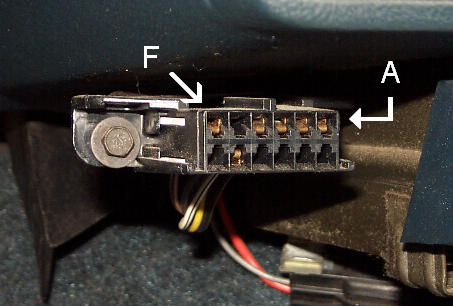
\includegraphics[width=.75\linewidth]{images/aldl.jpg}
  \caption{Conector \ac{ALDL}, creado por \textit{General Motors} antes de
  estandarizar OBD-II \cite{ReferenceManualChapter}.}
  \label{fig:aldl}
\end{figure}

No es hasta 1979 en que la \ac{SAE} recomienda crear un conector de
diagnóstico estandarizado en el mercado así como un conjunto de señales
de prueba. Finalmente, en 1991 la \ac{CARB} require que todos sus
vehículos tengan lo que sería el \ac{OBD}-I. Esta primera versión informaría
al conductor de un mal funcionamiento de alguno de los elementos del
vehículo mediante un \ac{MIL}, un indicador luminoso de fallos. Sin
embargo, solo se monitorizaban ciertos componentes relacionados con las
emisiones y no estaban calibrados \cite{SistemaOBD2Historia}.

Por ende, impulsado por las alertas \textit{smog} y por una fuerte regulación, en 1994
la \ac{CARB} obligó a todos los vehículos fabricados y vendidos a partir de 1996 incluir
el \ac{OBD}-II. Esto supuso un gran impulso en los mecanismos de monitorización de los
vehículos ya que además se estandarizó tanto el conector como los protocolos recomendados
por la \ac{SAE}. Tiempo más tarde, el Gobierno de los Estados Unidos aplicó la misma
medida a todos los vehículos del país \cite{SistemaOBD2Historia}.

Esta medida llegaría a Europa en 1998, según la Directiva 98/69EG, que obligaba a
todos los vehículos europeos a incluir dicho conector. Específicamente, los
automóviles de gasolina debían empezar a equiparlo en los modelos del año 2000; en el año 2003
para vehículos diésel; y en el año 2005 para camiones \cite{SistemaOBD2Historia}.

\subsection*{OBD--II}
\ac{OBD}--II es la segunda generación del sistema de diagnósticos de abordo, sucesor
de \ac{OBD}--I y su principal función es la de avisar al conductor cuando las
emisiones del vehículo son en torno a $1.5$ veces mayores de las diseñadas. A
diferencia de \ac{OBD}--I, \ac{OBD}--II también detecta fallos eléctricos, químicos
y mecánicos que puedan afectar al nivel de emisiones del vehículo (un caso típico
era un fallo químico del catalizador, indetectable por \ac{OBD}--I pero sí por la
segunda generación).

Este tipo de conector, al ser el primer estándar, cuenta con
múltiples interfaces que permiten conexiones mediante redes Wi-Fi, USB, Bluetooth,
etc. (cayendo pues en deshuso el protocolo de conexión por puerto serie -- RS232).
Esto se ha conseguido gracias al rápido avance de los sistemas embebidos, en donde
la combinación de \textit{software} y \textit{hardware} embebidos ha permitido que
cualquier usuario tenga acceso a este tipo de datos de forma relativamente simple
(actualmente, el conector más estandarizado es el controlador \texttt{ELM327} \cite{SistemaOBD2Historia},
figura \ref{fig:elm327}):

\begin{figure}[H]
  \centering
  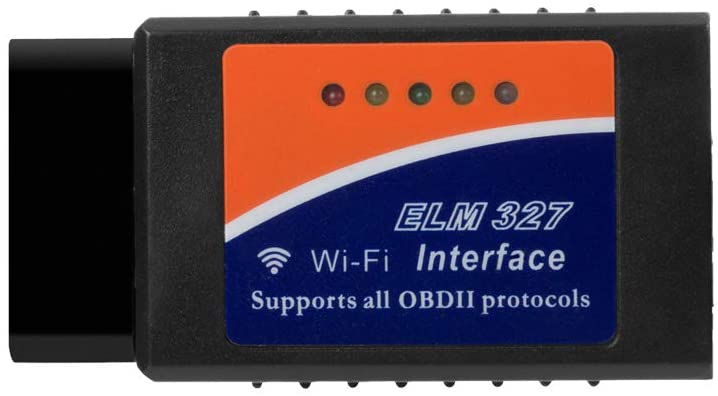
\includegraphics[width=.7\linewidth]{images/obd-ii-elm327.jpg}
  \caption{Controlador \texttt{ELM327} que cuenta con antenas Wi-Fi y Bluetooth para un acceso remoto \cite{AmazonComElm327}.}
  \label{fig:elm327}
\end{figure}

El sistema verifica todos los sensores directamente involucrados con las emisiones
del vehículo, como por ejemplo la inyección de aire al motor. Cuando algún sensor detecta
un fallo, se activa el \ac{MIL} indicando el fallo que sucede (o una combinación
de indicadores para notificar la existencia de un fallo, sin especificar exactamente
cuál).

El vehículo que incorpora un conector \ac{OBD}--II almacena la información sobre el
fallo del vehículo para que el mecánico que deba revisar el automóvil disponga de todos
los datos posibles. Por otra parte, este estándar permite una comunicación directa
con el vehículo mediante el envío de órdenes según un \ac{PID}. Por defecto, hay
una serie de \ac{PID}s estándar que la gran mayoría de vehículos deben incluir\footnote{%
Se dice ``la mayoría de vehículos'' porque hay ciertos \ac{PID}s que dependen
directamente del tipo de vehículo (a combustión, eléctrico, \dots) o del combustible
utilizado -- un vehículo eléctrico no ofrece información sobre las \ac{RPM} al igual
que un vehículo diésel no ofrece información sobre las bujías.}, pero también
los fabricantes de vehículos incluyen una serie de \ac{PID}s propios (conocidos como
\textit{\ac{PID}s propietarios}) que ofrecen información adaptada a cada vehículo
en particular y que, en principio, son privados y cerrados al público en general.

En Europa se implantó el \ac{EOBD}, la variación europea del estándar \ac{OBD}--II
implantada en el año 2000 en general. Si bien en apariencia es semejante al \ac{OBD}--II,
las diferencias radican en el \textit{software}. Por ejemplo, el estándar europeo
no monitoriza las evaporaciones del depósito de combustible; sin embargo, es más
sofisticado ya que usa ``mapas'' en las entradas de los sensores que obligan a que el
sensor se calibre empíricamente al sistema según las condiciones de operación del
motor (lo cual se traduce en que los sensores son mucho mejores pero más caros)
\cite{SistemaOBD2Historia}. Otra característica innovadora es que el sistema
europeo registra cuántos kilómetros se han recorrido desde que ha aparecido un
defecto \cite{EOBDOBD2}.

Finalmente, pero no menos importante, Japón tiene también su propio estándar denominado
\ac{JOBD}.

\subsection*{OBD--III}
El \ac{OBD}--III se espera que sea la siguiente versión del sistema que ya implementan
los coches actualmente. La principal diferencia con respecto a la versión anterior
será que el vehículo estará conectado de forma continua y emitiendo datos referentes
a las emisiones. De esta forma, se puede saber casi en el momento acerca de modificaciones
ilegales, un aumento en la contaminación del coche (signo de deterioro) y demás. No se
espera igualmente que sea un salto cualitativo ya que se sigue buscando que sea
altamente compatible con las herramientas que ya existen. Actualmente, se están
realizando pruebas en EE.UU. pero no hay cerrada ninguna fecha de estandarización
oficial por parte de los distintos continentes.

\subsection{Herramientas de monitorización y control del automóvil}
Pese al tiempo que lleva \ac{OBD}--II disponible, las herramientas existentes para
la actuación sobre un vehículo son relativamente escasas. La mayoría de modelos
presentes hoy en día en el mercado se basan directa o indirectamente en el
\texttt{ELM327}, un dispositivo de diagnóstico \ac{OBD} que cuenta con conexión
WiFi, Bluetooth y serie para la lectura local.

Por lo general, las herramientas que hay se utilizan por mecánicos o fanáticos del
sector para acceder a la información del estado del vehículo y ver los errores que
pudiera tener. Sin embargo, tras una breve documentación sobre el tema, la mayoría
de los casos buscaban directamente monitorizar en el momento el estado
del vehículo para obtener información relativa a los consumos, contaminación,
etc.

Por ejemplo, en el trabajo de Rimpas \textit{et al.} \cite{rimpasOBDIISensorDiagnostics2020}, se utiliza
un sensor \texttt{ELM327} para verificar que la información proporcionada por
el puerto del vehículo y la presentada por la telemetría presente en el mismo
(velocímetro y tacómetro) son coherentes entre sí (previa adaptación de los
valores en \textit{bytes} presentados por el conector a valores legibles). En
dicha investigación se llega a la conclusión de que el conector \ac{OBD}--II obtiene
valores fiables y consistentes tanto con los mostrados por el propio vehículo
como los proporcionados por el fabricante.

Otro tipo de investigaciones llevadas a cabo gracias a la presencia de este conector
en los automóviles es la de la caracterización de conductores y hábitos de conducción
según la telemetría reportada por el vehículo. En el estudio realizado por
Galih Hermawan y Emir Husni \cite{hermawanAcquisitionModelingEvaluating2020} se
estudia la combinación de la lectura de los sensores mediante el \ac{OBD}--II con
vehículos que presentan el sistema \ac{ADAS}.
El estudio busca identificar hábitos de conducción según la lectura de los diversos
sensores que hay en el sistema. También persigue detectar quién es el conductor que
está llevando el vehículo actualmente. En el estudio, el uso de \ac{OBD}--II junto
con los algoritmos de los \textit{k--Nearest Neighbor} (k--NN) y \textit{Naive Bayes}
consiguieron una precisión en la identificación del 100\% (
para un conjunto de datos de 10 conductores).
Por otra parte, el uso de inteligencia artificial junto con técnicas de \textit{clustering}
permitieron identificar comportamientos de los conductores al volante y relacionarlo
además con situaciones de riesgo y peligro. Además, se ha aplicado a otras características
también interesantes como detectar el tipo de calzada, predecir el tiempo de viaje,
analizar el consumo del vehículo y demás. El esquema seguido en la investigación es el
que se presenta en la figura \ref{fig:investigation-scheme}:

\begin{figure}[H]
  \centering
  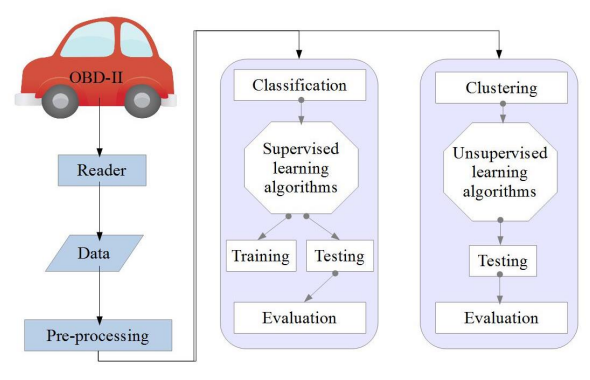
\includegraphics[width=.7\linewidth]{images/general-scheme-investigation.png}
  \caption{Esquema seguido para determinar los hábitos de conducción usando el \ac{OBD}--II \cite{hermawanAcquisitionModelingEvaluating2020}.}
  \label{fig:investigation-scheme}
\end{figure}

Por último, uno de los tipos de investigación bastante interesante realizada en los
últimos años es la de la generación de perfiles de conducción y de consumo. En el
artículo realizado por Ameen \textit{et al.} \cite{husseinaliameenDrivingBehaviourIdentification2021}
se define un sistema de clasificación del comportamiento del conductor al volante
(que es además el que se propone usar en este proyecto) el cual combina los datos
recibidos por el \ac{OBD}--II y del \ac{GPS} (figura \ref{fig:driving-behaviour}):

\begin{figure}[H]
  \centering
  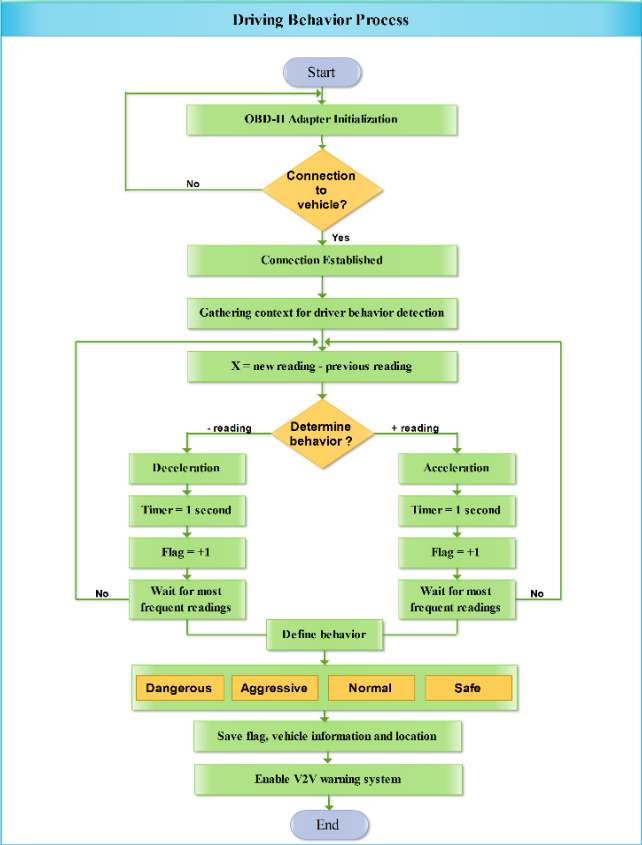
\includegraphics[width=.7\linewidth]{images/driving-behaviour-workflow.png}
  \caption{Flujo de análisis para determinar el comportamiento al volante de un conductor \cite{husseinaliameenDrivingBehaviourIdentification2021}.}
  \label{fig:driving-behaviour}
\end{figure}

Al final, el estudio concluía con los siguientes perfiles de conducción:

\begin{itemize}
  \item \textbf{Peligroso}, para una aceleración en general superior a $7\ \nicefrac{m}{s^2}$.
  \item \textbf{Agresivo}, para una aceleración entre $\left[4\ \nicefrac{m}{s^2}, 7\ \nicefrac{m}{s^2}\right)$.
  \item \textbf{Normal}, para una aceleración entre $\left[2\ \nicefrac{m}{s^2}, 4\ \nicefrac{m}{s^2}\right)$.
  \item \textbf{Seguro}, para una aceleración entre $\left[0\ \nicefrac{m}{s^2}, 2\ \nicefrac{m}{s^2}\right)$.
\end{itemize}

\section{Objetivos del desarrollo del proyecto}\label{sec:objectives}
Como se ha podido apreciar, existen multitud de aplicaciones relacionadas directa
o indirectamente con el \ac{OBD}--II, en parte por la longevidad del conector
en el mercado.

Sin embargo, todas o la gran mayoría de aplicaciones están destinadas a los profesionales
del sector, e incluso se ha aprovechado este conector para dificultar el acceso a
los datos del vehículo, habiendo de ir a un taller oficial para que puedan hacer
las reparaciones pertinentes.

Por otra parte, el parque de vehículos español es cada año más viejo debido a
diversos factores que no se van a analizar en este trabajo. Esto implica que cada
año más y más vehículos pierden el soporte por parte del fabricante y se vuelven
cada vez más costosos y complejos de mantener.

Para los no eruditos, el mundo del automóvil es el gran desconocido en donde una
serie de personas cualificadas se encargan del mantenimiento y correcto funcionamiento
del mecanismo que nos transporta por el mundo. Si bien es cierto que es necesaria
esta figura, hay una serie de buenas prácticas y actuaciones que pueden prevenir
tener que ir al mecánico de forma recurrente. Solo hace falta acceso a la información
de manera accesible.

Es por esto que nace \ac{VIMS}, un proyecto que pretende desarrollar un sistema completo
que consta de varias partes: un dispositivo embebido, un servidor y el usuario en sí
(figura \ref{fig:general-scheme}):

\begin{figure}[H]
  \centering
  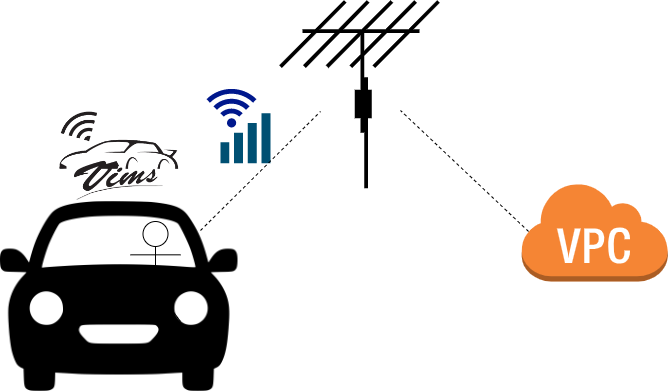
\includegraphics[width=\linewidth]{images/general-scheme.png}
  \caption{Esquema general que modela el modo de funcionamiento del sistema.}
  \label{fig:general-scheme}
\end{figure}

La idea fundamental detrás de este proyecto es la de devolverle a los usuarios
el control sobre su vehículo, ser conscientes de cómo funciona o, al menos, entender
mejor qué pueden hacer para mejorar tanto su estilo de conducción como la seguridad
al volante. De esta forma, con el dispositivo se espera también prevenir riesgos
ya que los propietarios y usuarios de los vehículos estarán informados en todo
momento de qué error pueda tener.

Como se prevé que este dispositivo sea utilizado por una gran variedad de usuarios
es crucial que sea accesible en términos de sencillez de manejo, entendimiento y
uso: evitar datos excesivamente técnicos, presentar la información más relevante
primero, etc.

Para ello, se hará uso de plataformas en la nube para gestionar, almacenar y presentar
la información al usuario y se contará con una aplicación móvil que permita un
fácil acceso a los datos del vehículo, tanto históricos como generados en el momento.

Al igual que otros trabajos previamente realizados, el proyecto se realiza sobre
las filosofías del código libre y del \textit{hardware} libre, que se traduce en
que todos los recursos (tanto físicos como \textit{software}) estarán disponibles
enteramente para cualquier persona interesada en ver cómo funciona, replicar el
proyecto por su cuenta y contar con plena potestad para mejorarlo, redistribuirlo
y trabajar con él (siempre bajo un prisma de reconocimiento al autor original
del trabajo regido por \textit{copyright}). Para ello, se ha decidido hacer uso
de la licencia MIT\footnote{Se pueden obtener más detalles sobre la licencia MIT
en la siguiente URL: \url{https://choosealicense.com/licenses/mit/}}.

\section{Metodología}\label{sec:methodology}
El proyecto que se pretende desarrollar es un proyecto de ingeniería. Esto se
traduce en que la metodología y la forma de trabajo son pilares fundamentales
en el desarrollo del mismo.

El primer paso realizado fue el de recopilar recursos e información de qué
necesitaban específicamente los usuarios. Para ello, se elaboró un cuestionario
en donde de forma general se preguntaba a conductores y no conductores qué querrían
tener en su vehículo. Los primeros sirvieron de grupo de control, los segundos para
aumentar la entropía de los datos obtenidos. El primer análisis realizado se detalla
en la sección \ref{ssec:user-req}, de la especificación de requisitos. Posteriormente,
en el punto \ref{chap:merch} se analiza en mayor profundidad los datos obtenidos
y se extraerán conclusiones.

A continuación, se realizó un estudio sobre qué plataformas y dispositivos están
accesibles de forma global para la generación y transmisión de datos. Esta fase
se centró principalmente en ``descubrir'' variantes del modelo ESP32 que incluyesen
ciertas antenas para permitir una mayor conectividad. Tras valorar diversas opciones,
se decidió usar el LILYGO T-SIM7000G ESP32 que incluye soporte de forma nativa para
tarjetas microSD, antena \ac{LTE}, alimentación externa por batería, antena \ac{GPS}, WiFi y
Bluetooth.

Una vez se decidió que dispositivo físico se iba a utilizar, se comenzó con el desarrollo
de los distintos diagramas que modelan el sistema, tanto lógicos como de diseño. Esta
parte fue crucial para asentar las bases de lo que será el proyecto y ha permitido seguir
el avance del mismo.

Por último, se realizó el serigrafiado de la placa y se comenzó la implementación
física de los diseños realizados. Sin embargo, esta etapa no se ha podido completar
por distintos contratiempos que se comentan en más detalle en el punto \ref{chap:planification}.


%% Product description
\chapter{Estructura del proyecto}\label{chap:structure}
El desarrollo del sistema \ac{VIMS} es un proceso multidisciplinar en el que se deben
desarrollar varias áreas de conocimiento. Este proyecto se ha postulado como
un desarrollo integral de ingeniería y es por eso por lo que está dividido en
varios bloques que conforman un factor clave en el desarrollo del mismo.

En este proyecto existen diversos bloques diferenciados: un estudio de mercado y de
las características de los usuarios, un estudio matemático asociado a la lectura de
valores y adecuación del \textit{hardware}, el proceso de diseño \textit{hardware}
en sí, el diseño \textit{software} del sistema y el análisis de planificación del mismo.

\begin{itemize}
  \item El estudio de mercado pretende averiguar y formalizar las necesidades de los
  conductores y usuarios de la vía. Es la primera aproximación y facilita la
  delimitación del producto y, sobre todo, ofrecerle al usuario final algo de utilidad
  y que pueda necesitar.
  \item El estudio matemático se encarga de investigar la ``traducción'' de los
  valores recibidos por el vehículo (según los datos asociados al estudio de mercado
  realizado con anterioridad).
  \item El diseño \textit{software} modela principalmente cómo se va a estructurar
  el sistema y cómo debe comportarse ante los distintos eventos que puede recibir.
  Esta fase conlleva realizar diagramas lógicos y de diseño del sistema en su conjunto.
  \item El diseño \textit{hardware} conlleva tanto el estudio de los componentes del
  sistema así como de las restricciones físicas del mismo. Además, en esta sección
  también se introduce el diseño 3D de la caja que alojará la placa.
  \item El análisis de planificabilidad complementa el diseño \textit{software}
  y estudia si el sistema es planificable. En los requisitos no se define \ac{VIMS}
  como un sistema en tiempo real, pero la cantidad de componentes que contiene y las
  acciones que tiene que realizar requieren del uso de subrutinas y de una planificación
  previa para asegurar un correcto funcionamiento del mismo.
\end{itemize}

Es importante detallar que pese a que el sistema se compone de varios componentes,
son dos los principales que lo caracterizan:

\begin{enumerate}
  \item La placa, \ac{VIMS}, que va embebida en los vehículos del sistema. Se encarga
  de toda la lectura, adaptación y emisión de datos. Además, cuenta con soporte para
  poder realizar una transmisión de la información a un dispositivo asociado mediante
  redes \ac{PAN}.
  \item El servidor \textit{cloud}, el ``cerebro'' encargado de recibir las tramas,
  los datos y la información relativa a las placas \ac{VIMS}, los dispositivos de
  usuario y demás componentes. Además, tiene la responsabilidad de ofrecer a los
  usuarios una \ac{GUI}, generar información relevante a partir de los datos (como
  estadísticas), gestionar las suscripciones y enviar periódicamente la información
  al usuario.
\end{enumerate}

\section{Estudio de mercado}\label{sec:merch}
Para el desarrollo de este proyecto, se hizo un estudio de mercado tanto de los
consumidores como de sus características, además de una evaluación exhaustiva
de qué les gustaría tener en su vehículo.

Este proyecto pretende en un futuro salir a mercado y suplir características que los
usuarios echan en falta en sus correspondientes medios de transporte. Como en principio
funciona con cualquier vehículo que cuente con \ac{OBD}--II, las respuestas no se han
limitado a aquellos conductores que condujesen turismos sino cualquier tipo de
automóvil: motocicleta, camión, etc.

Es importante destacar que el estudio tiene varios sesgos que han restringido
y delimitado las respuestas que se han registrado:

\begin{enumerate}
  \item Se ha realizado un cuestionario usando Google Forms, una plataforma de Google
        que permite preparar una serie de preguntas y respuestas y aplicar ciertos
        filtros sobre ellas. Por ejemplo, para aquellos que dijeron ser conductores,
        se hicieron preguntas diferentes frente a quienes no lo fueran.

        Esto permite obtener datos más fidedignos y acotados según la población que
        respondiera. Sin embargo, tiene una limitación implícita: restringe el acceso
        a aquellos con conocimientos ``suficientes'' acerca de la plataforma. Pese
        a que el producto pretende ser lo más accesible posible, no hay que olvidar
        que este tipo de tecnologías permanecen desconocidas para una gran parte
        de la población con escasos conocimientos acerca de Internet o de las
        nuevas tecnologías. Se comentará más adelante, pero esto se ve reflejado
        principalmente en la edad media de quienes respondieron el cuestionario.

        Por otra parte, al ser un cuestionario aparece otra limitación implícita
        y es la validación y verificación de las respuestas: se confía en la buena
        fe de los participantes y en la calidad de sus respuestas. Igualmente, se
        desarrolló el cuestionario junto con una psicóloga que ayudó a definir
        preguntas cerradas e incluir ciertas respuestas de control. Por otra parte,
        se usó el propio mecanismo que ofrece este servicio de Google para ordenar
        aleatoriamente las respuestas del cuestionario (y que eso sirviese también
        como control).

  \item Los encuestados fueron contactados principalmente por la red social Twitter,
        mediante la difusión con ``me gusta'' y ``retweet''. También se usaron otros
        medios de comunicación (como el correo UPM y Telegram/WhatsApp), pero el
        mayoritario fue el ya mencionado. Nuevamente, esto introduce un sesgo tanto
        por edad como por accesibilidad.

  \item Junto con la encuesta, se realizó un sorteo entre aquellos que respondiesen
        a la misma de un cheque regalo de Amazon valorado en 20\EUR{}. Si bien este
        incentivo pudiera resultar interesante, puede resultar también en un nuevo
        sesgo en donde personas que o bien no compren en Amazon o bien no sepan
        lo que es no quisieran hacer el cuestionario.

        Además, se plantea la casuística en que ciertas personas quisieran responder
        al cuestionario solo por el cheque de Amazon, sin importar la calidad de
        las respuestas, ``ensuciando'' los resultados obtenidos y quitándole credibilidad
        al cuestionario en sí.

        Esto se analizará posteriormente junto con las respuestas recibidas y las
        preguntas de control introducidas.

  \item El cuestionario, al ser relativamente exhaustivo, pudo echar para atrás a muchos
        posibles encuestados ya que se estima que el tiempo medio para realizarlo es del
        orden de 10/15 minutos. A parte del daño evidente de tener menos muestra con la
        que trabajar, este posible suceso reduciría también la variedad de la población
        y la calidad del estudio realizado.
\end{enumerate}

La primera pregunta que se realizó a los encuestados era si eran conductores o no.
Los datos revelan que el $72.7\%$ ($16$) de los encuestados son conductores, mientras que el
$27.3\%$ ($6$) restantes no, del total que fueron $22$ (figura \ref{fig:drivers-nodrivers}):

\begin{figure}[H]
  \centering
  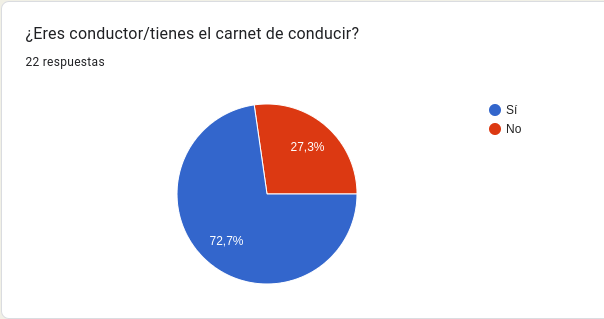
\includegraphics[width=\linewidth]{images/drivers-nodrivers.png}
  \caption{Gráfico de tarta que muestra quiénes de los encuestados son conductores ($72.7\%$) y quiénes no ($27.3\%$).}
  \label{fig:drivers-nodrivers}
\end{figure}

Sobre aquellos que dijeron ser conductores, se preguntó acerca de los años que
llevaban con carnet de conducir, así como los tipos de carnet de conducir que tenían
los encuestados.

Se vio que un $68.8\%$ tenía el carnet desde hace 3 años o más ($11$ encuestados
en particular); un $12.5\%$ tenía el carnet desde hace solo un año ($2$ encuestados)
y el restante, en su mayoría, tenía el carnet desde hace menos de un año. Esto se ve
reflejado en el histograma \ref{fig:carnet-time-hist}:

\begin{figure}[H]
  \centering
  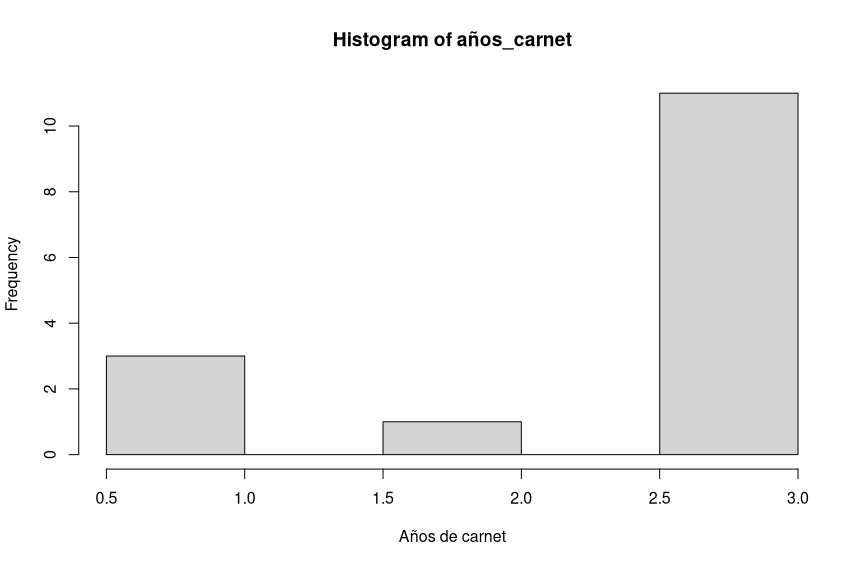
\includegraphics[width=\linewidth]{images/carnet-time.png}
  \caption{Histograma que muestra los años de carnet de los encuestados.}
  \label{fig:carnet-time-hist}
\end{figure}

Con respecto a los tipos de carnet, el $100\%$ de los encuestados (que dijeron ser
conductores) tiene el carnet tipo B. Se vio además que el $18.8\%$ tiene además los
carnets relativos a las motocicletas (muy posiblemente, los encuestados tienen el
carnet tipo ``A'' que les habilita automáticamente para aquellos de menor nivel,
como el AM, A1 y A2); y únicamente un encuestado tiene el carnet tipo C, que permite
conducir camiones.

Una restricción que se comentó con anterioridad era la edad media de los participantes.
Esta pregunta se realizó por dos motivos:

\begin{enumerate}
  \item Definir estadísticamente la edad media de la población para una posterior evaluación
        de su longevidad y experiencia tanto en la conducción como en la posible
        compra-venta de vehículos.
  \item Diferenciar, definir y clasificar los encuestados por grupos de edad y descubrir
        posibles sesgos y restricciones en las respuestas para un posterior análisis
        sobre la causa de dichos sesgos y restricciones.
\end{enumerate}

Es necesario decir que solo se preguntó por la edad a aquellas personas que respondieron
afirmativamente a ser conductores. Esto se hizo así debido a que sus respuestas han
conformado el dato más relativo a la hora de realizar la investigación, y se hace así
también estadísticamente.

Se tiene pues que:

\begin{equation}\label{eq:ages}
  \left\{\begin{aligned}
    X_{min}               & = 19     \\
    \bar{X}               & = 30     \\
    Mediana\left(X\right) & = 26.5   \\
    S\left(X\right)       & = 10.564 \\
    X_{max}               & = 55
  \end{aligned}\right.
\end{equation}

Se construyó además un gráfico de tarta (figura \ref{fig:ages}) que muestra cómo
quedan distribuidas las edades de los participantes:

\begin{figure}[H]
  \centering
  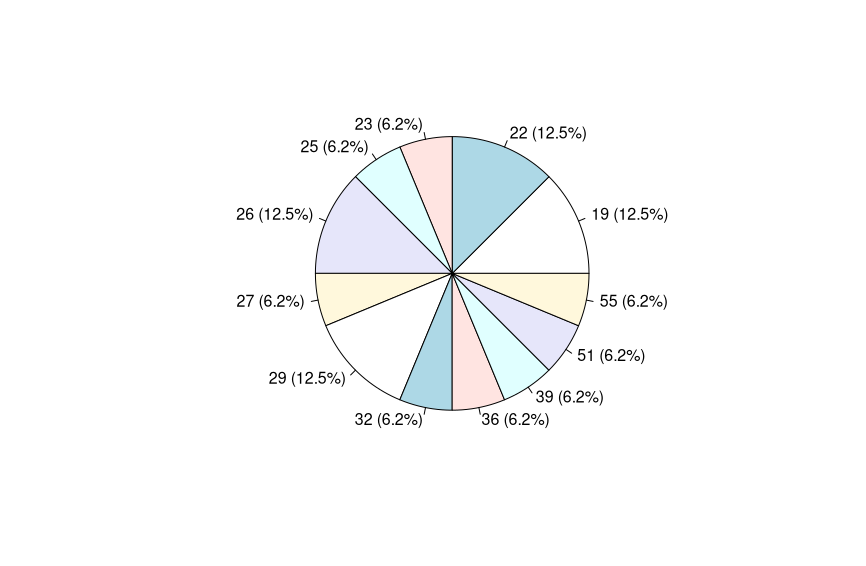
\includegraphics[width=\linewidth]{images/ages-pie.png}
  \caption{Gráfico de tarta que muestra la distribución de edades (valor previo al paréntesis) y su frecuencia en porcentaje.}
  \label{fig:ages}
\end{figure}

Como se puede ver en la ecuación \ref{eq:ages}, la distancia entre los valores
mínimo y máximo es de $36$ puntos. Sin embargo, los valores de la media $\left(\bar{X}\right)$
y la mediana $\left(Mediana\left(X\right)\right)$ muestran que la distribución está
bastante centrada en torno a la media, con una desviación estándar $\left(S\left(X\right)\right)$
de $\approx\pm10.564$.

Es interesante notar los tres grandes bloques presentes en la figura \ref{fig:ages}
que evidencian lo que se venía indicando anteriormente: en proporción, a la encuesta
ha accedido más población joven que adulta. Mismamente, solo el porcentaje de personas
encuestadas con edad por debajo de los 26 años es del $49.9\%$, casi la mitad de
los encuestados. Ampliando dicho margen hasta los 36 años, el porcentaje crece hasta
el $81 \%$.

Este dato se puede ver también reflejado en la distribución de los cuartiles, en donde
se tiene que:

\begin{equation}\label{eq:age-quartiles}
  \left\{
  \begin{aligned}
    Q_1 & = 22.75 \\
    Q_3 & = 33.00
  \end{aligned}
  \right.
\end{equation}

Como se puede apreciar en la ecuación \ref{eq:age-quartiles}, la distribución de
cuartiles está en un rango de edad por debajo de los 33 años para el $75\%$ de la
muestra, indicativo nuevamente de una población encuestada joven.

Destacan dos datos sobre los demás en donde los encuestados tienen 51 y 55 años
respectivamente. De este caso en particular se hablará posteriormente, pero cabe
destacar que sus respuestas fueron las más pobres en cuanto a contenido (sobre todo
en aquellas que sirvieron de control), seguramente debido al formato del
cuestionario, fatiga tras responder las secciones anteriores, etc.

Una vez se indagó acerca de la información que identifica a la muestra, se preguntó
directamente por el vehículo con el que contaban así como las características del
mismo. Para esta sección, se han dividido las preguntas en tres categorías:
\textit{básico}, \textit{habitual} y \textit{premium}. Dichas categorías se crean
según el porcentaje de uso habitual mundial de las características que se
enumeran en la tabla \ref{tab:car-specs}:

\begin{table}[H]
  \centering
  \begin{tabular}{|c|c|c|}
    \hline
    \textbf{Básico}          & \textbf{Habitual}            & \textit{\textbf{Premium}} \\
    \hline\hline
    Control de crucero       & Pantalla táctil              & Asistente virtual         \\
    Limitador de velocidad   & GPS                          & Aplicación móvil          \\
    Cámara de visión trasera & Detección de ángulos muertos & Cámara \textit{on-board}  \\
    Botón de arranque        & Android Auto                 &                           \\
    \hline
  \end{tabular}
  \caption{Tabla de distribución de las características de los vehículos, preguntado en el cuestionario.}
  \label{tab:car-specs}
\end{table}

Tras el cuestionario, las frecuencias obtenidas fueron:

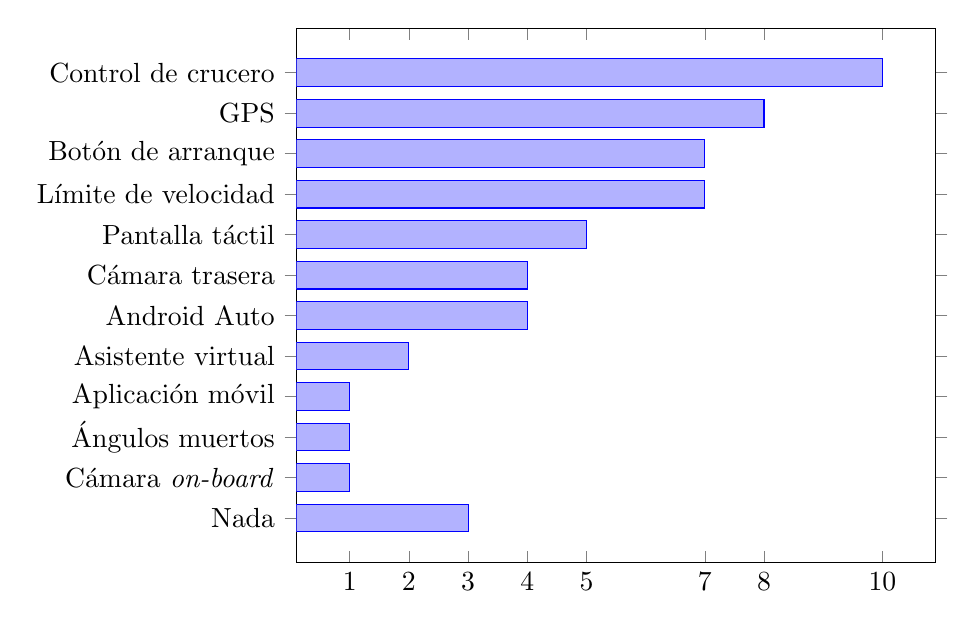
\begin{tikzpicture}
  \begin{axis} [%
      xbar,
      width=.8\linewidth,
      ytick=data,
      yticklabels={%
          Nada,
          Cámara \textit{on-board},
          Ángulos muertos,
          Aplicación móvil,
          Asistente virtual,
          Android Auto,
          Cámara trasera,
          Pantalla táctil,
          Límite de velocidad,
          Botón de arranque,
          GPS,
          Control de crucero,
        },
      xtick=data,
    ]
    \addplot coordinates {
        (3, 0)
        (1, 1)
        (1, 2)
        (1, 3)
        (2, 4)
        (4, 5)
        (4, 6)
        (5, 7)
        (7, 8)
        (7, 9)
        (8, 10)
        (10, 11)
      };
  \end{axis}
\end{tikzpicture}

\section{Estudio matemático}\label{sec:maths}
El estudio matemático va muy ligado al punto anterior (\ref{sec:merch}) ya que se
analizan los parámetros de \ac{OBD}--II y su ecuación matemática para obtener un
valor en $\mathbb{R}$ entendible por las personas.

Antes de dar paso a las ecuaciones en sí, es importante entender cómo funciona
el conector \ac{OBD}--II en esta situación. Los datos enviados y recibidos por
el coche están siempre codificados en un valor binario, recogido en un vector
de cuatro elementos en donde cada elemento tiene un \textit{byte} de tamaño. De
esta forma, se define al valor obtenido tras leer el conector \ac{OBD}--II como:

\begin{table}[H]
  \centering
  \resizebox{\textwidth}{!}{\begin{tabular}{|c|c|c|c|c|c|c|c|c|c|c|c|c|c|c|c|c|c|c|c|c|c|c|c|c|c|c|c|c|c|c|c|}
      \hline
      \multicolumn{8}{|c|}{$A$} & \multicolumn{8}{|c|}{$B$} & \multicolumn{8}{|c|}{$C$} & \multicolumn{8}{|c|}{$D$}                                                                                                                                                                                                                                 \\
      \hline
      $A_7$                     & $A_6$                     & $A_5$                     & $A_4$                     & $A_3$ & $A_2$ & $A_1$ & $A_0$ & $B_7$ & $B_6$ & $B_5$ & $B_4$ & $B_3$ & $B_2$ & $B_1$ & $B_0$ & $C_7$ & $C_6$ & $C_5$ & $C_4$ & $C_3$ & $C_2$ & $C_1$ & $C_0$ & $D_7$ & $D_6$ & $D_5$ & $D_4$ & $D_3$ & $D_2$ & $D_1$ & $D_0$ \\
      \hline
    \end{tabular}}
  \caption{Vector de \textit{bytes} que representa los datos recibidos del conector \ac{OBD}--II \cite{OBDIIPIDs2021}.}
  \label{tab:byte-array}
\end{table}

De esta forma, cuando se escribe $A_4$ se hace referencia al cuarto bit
del vector $A$. Los bits están ordenados según \ac{MSB}, de forma que
$A_7$ es el bit más significativo y $A_0$ el menor.

Los datos se obtienen del \ac{OBD}--II utilizando un lenguaje estándar llamado
\ac{PID}. El \ac{PID} se codifica como un número entero de 16 bits en donde los 8
primeros bits identifican el servicio/modo y los 8 restantes la operación a realizar.
Actualmente, están registrados los siguientes modos de funcionamiento (tabla
\ref{tab:pids-mode}):

\begin{table}[H]
  \centering
  \begin{tabularx}{\textwidth}{ | c | X | }
    \hline
    \textbf{Modo (hex)} & \textbf{Descripción}                                                                       \\
    \hline
    \texttt{01}         & Muestra los datos actuales del vehículo                                                    \\
    \hline
    \texttt{02}         & Muestra los datos almacenados del cuadro del vehículo                                      \\
    \hline
    \texttt{03}         & Muestra los códigos \ac{DTC}                                                               \\
    \hline
    \texttt{04}         & Elimina los códigos \ac{DTC} almacenados                                                   \\
    \hline
    \texttt{05}         & Resultados del test del sensor de oxígeno (sin \ac{CAN})                                   \\
    \hline
    \texttt{06}         & Resultados del test del sensor de oxígeno (con \ac{CAN})                                   \\
    \hline
    \texttt{07}         & Muestra los códigos \ac{DTC} pendientes (eliminados durante el último ciclo de conducción) \\
    \hline
    \texttt{08}         & Operaciones de control sobre los componentes del sistema                                   \\
    \hline
    \texttt{09}         & Petición de información sobre el vehículo                                                  \\
    \hline
    \texttt{0A}         & Códigos \ac{DTC} eliminados                                                                \\
    \hline
  \end{tabularx}
  \caption{Lista de modos de funcionamiento del estándar \ac{OBD}--II \cite{OBDIIPIDs2021}.}
  \label{tab:pids-mode}
\end{table}

Es importante destacar que no todos los fabricantes tienen por qué soportar todos
los modos, y que además ciertos fabricantes pueden definir sus modos propios por encima
del valor \texttt{09}.

Todos los modos definidos anteriormente tienen un conjunto de órdenes de soporte
en donde el sistema indica qué \ac{PID}s están soportados y cuáles no, por cada 32
\ac{PID}s. Por ejemplo, enviar la orden \texttt{0x0100} (\textit{modo 1, PID 0})
devolverá un valor que representará si los siguientes 32 \ac{PID}s están soportados.
Si el valor fuese, por ejemplo, \texttt{BE1FA813} se tendría que:

\begin{table}[H]
  \centering
  \resizebox{\textwidth}{!}{\begin{tabular}{ | c | c | c | c | c | c | c | c | c | c | c | c | c | c | c | c | c | c | c | c | c | c | c | c | c | c | c | c | c | c | c | c | c | }
      \hline
      \textbf{Hexadecimal} & \multicolumn{4}{|c|}{\texttt{B}} & \multicolumn{4}{|c|}{\texttt{E}} & \multicolumn{4}{|c|}{\texttt{1}} & \multicolumn{4}{|c|}{\texttt{F}} & \multicolumn{4}{|c|}{\texttt{A}} & \multicolumn{4}{|c|}{\texttt{8}} & \multicolumn{4}{|c|}{\texttt{1}} & \multicolumn{4}{|c|}{\texttt{3}}                                                                                                                                                                                                                                                                                                                                                 \\
      \hline
      \textbf{Binario}     & \texttt{1}                       & \texttt{0}                       & \texttt{1}                       & \texttt{1}                       & \texttt{1}                       & \texttt{1}                       & \texttt{1}                       & \texttt{0}                       & \texttt{0}  & \texttt{0}  & \texttt{0}  & \texttt{1}  & \texttt{1}  & \texttt{1}  & \texttt{1}  & \texttt{1}  & \texttt{1}  & \texttt{0}  & \texttt{1}  & \texttt{0}  & \texttt{1}  & \texttt{0}  & \texttt{0}  & \texttt{0}  & \texttt{0}  & \texttt{0}  & \texttt{0}  & \texttt{1}  & \texttt{0}  & \texttt{0}  & \texttt{1}  & \texttt{1}  \\
      \hline
      \textbf{?`Soportado?} & \done                            & \wontfix                         & \done                            & \done                            & \done                            & \done                            & \done                            & \wontfix                         & \wontfix    & \wontfix    & \wontfix    & \done       & \done       & \done       & \done       & \done       & \done       & \wontfix    & \done       & \wontfix    & \done       & \wontfix    & \wontfix    & \wontfix    & \wontfix    & \wontfix    & \wontfix    & \done       & \wontfix    & \wontfix    & \done       & \done       \\
      \hline
      \textbf{PID}         & \texttt{01}                      & \texttt{02}                      & \texttt{03}                      & \texttt{04}                      & \texttt{05}                      & \texttt{06}                      & \texttt{07}                      & \texttt{08}                      & \texttt{09} & \texttt{0A} & \texttt{0B} & \texttt{0C} & \texttt{0D} & \texttt{0E} & \texttt{0F} & \texttt{10} & \texttt{11} & \texttt{12} & \texttt{13} & \texttt{14} & \texttt{15} & \texttt{16} & \texttt{17} & \texttt{18} & \texttt{19} & \texttt{1A} & \texttt{1B} & \texttt{1C} & \texttt{1D} & \texttt{1E} & \texttt{1F} & \texttt{20} \\
      \hline
    \end{tabular}}
  \caption{Obtención de los \ac{PID}s soportados según el modo \cite{OBDIIPIDs2021}.}
  \label{tab:supported-pids}
\end{table}

A continuación, se dejan un conjunto de \ac{PID}s que se van a implementar en el
proyecto así como el código de acceso a ellos y la ecuación que permite obtener el
valor real.

\subsection*{Modo \texttt{01}}
Este modo permite acceder a la información en tiempo real del vehículo, según se
está en marcha. Los datos a los que se accede son:

\begin{table}[H]
  \centering
  \begin{tabularx}{\textwidth}{|c|X|}
    \hline
    \textbf{PID (hex)}       & \texttt{04}                    \\
    \hline
    \textbf{Bytes devueltos} & $1$                            \\
    \hline
    \textbf{Descripción}     & Carga del motor, en porcentaje \\
    \hline
    \textbf{Valor mínimo}    & $0\%$                          \\
    \hline
    \textbf{Valor máximo}    & $100\%$                        \\
    \hline
    \textbf{Fórmula}         &                                %
    \begin{equation*}
      \frac{A}{2.55}
    \end{equation*}                                 \\
    \hline
  \end{tabularx}
  \caption{\ac{PID} \texttt{04} -- carga del motor, en $\%$.}
\end{table}

\begin{table}[H]
  \centering
  \begin{tabularx}{\textwidth}{|c|X|}
    \hline
    \textbf{PID (hex)}       & \texttt{05}                            \\
    \hline
    \textbf{Bytes devueltos} & $1$                                    \\
    \hline
    \textbf{Descripción}     & Temperatura del refrigerante del motor \\
    \hline
    \textbf{Valor mínimo}    & $-40~\tccentigrade$                    \\
    \hline
    \textbf{Valor máximo}    & $215~\tccentigrade$                    \\
    \hline
    \textbf{Fórmula}         &                                        %
    \begin{equation*}
      A - 40
    \end{equation*}                                         \\
    \hline
  \end{tabularx}
  \caption{\ac{PID} \texttt{05} -- temperatura del refrigerante del motor, en $\tccentigrade$.}
\end{table}

\begin{table}[H]
  \centering
  \begin{tabularx}{\textwidth}{|c|X|}
    \hline
    \textbf{PID (hex)}       & \texttt{0C}         \\
    \hline
    \textbf{Bytes devueltos} & $2$                 \\
    \hline
    \textbf{Descripción}     & Velocidad del motor \\
    \hline
    \textbf{Valor mínimo}    & $0~RPM$             \\
    \hline
    \textbf{Valor máximo}    & $16383.75~RPM$      \\
    \hline
    \textbf{Fórmula}         &                     %
    \begin{equation*}
      \frac{256A + B}{4}
    \end{equation*}                      \\
    \hline
  \end{tabularx}
  \caption{\ac{PID} \texttt{0C} -- velocidad del motor, en $RPM$.}
\end{table}

\begin{table}[H]
  \centering
  \begin{tabularx}{\textwidth}{|c|X|}
    \hline
    \textbf{PID (hex)}       & \texttt{0D}            \\
    \hline
    \textbf{Bytes devueltos} & $1$                    \\
    \hline
    \textbf{Descripción}     & Velocidad del vehículo \\
    \hline
    \textbf{Valor mínimo}    & $0~\nicefrac{km}{h}$   \\
    \hline
    \textbf{Valor máximo}    & $255~\nicefrac{km}{h}$ \\
    \hline
    \textbf{Fórmula}         &                        %
    \begin{equation*}
      A
    \end{equation*}                         \\
    \hline
  \end{tabularx}
  \caption{\ac{PID} \texttt{0D} -- velocidad del vehículo, en $\nicefrac{km}{h}$.}
\end{table}

\begin{table}[H]
  \centering
  \begin{tabularx}{\textwidth}{|c|X|}
    \hline
    \textbf{PID (hex)}       & \texttt{11}             \\
    \hline
    \textbf{Bytes devueltos} & $1$                     \\
    \hline
    \textbf{Descripción}     & Posición del acelerador \\
    \hline
    \textbf{Valor mínimo}    & $0\%$                   \\
    \hline
    \textbf{Valor máximo}    & $100\%$                 \\
    \hline
    \textbf{Fórmula}         &                         %
    \begin{equation*}
      \frac{A}{2.55}
    \end{equation*}                          \\
    \hline
  \end{tabularx}
  \caption{\ac{PID} \texttt{11} -- posición del acelerador, en $\%$.}
\end{table}

\begin{table}[H]
  \centering
  \begin{tabularx}{\textwidth}{|c|X|}
    \hline
    \textbf{PID (hex)}       & \texttt{2F}                      \\
    \hline
    \textbf{Bytes devueltos} & $1$                              \\
    \hline
    \textbf{Descripción}     & Nivel del tanque del combustible \\
    \hline
    \textbf{Valor mínimo}    & $0\%$                            \\
    \hline
    \textbf{Valor máximo}    & $100\%$                          \\
    \hline
    \textbf{Fórmula}         &                                  %
    \begin{equation*}
      \frac{A}{2.55}
    \end{equation*}                                   \\
    \hline
  \end{tabularx}
  \caption{\ac{PID} \texttt{2F} -- nivel del tanque del combustible, en $\%$.}
\end{table}

\begin{table}[H]
  \centering
  \begin{tabularx}{\textwidth}{|c|X|}
    \hline
    \textbf{PID (hex)}       & \texttt{46}          \\
    \hline
    \textbf{Bytes devueltos} & $1$                  \\
    \hline
    \textbf{Descripción}     & Temperatura ambiente \\
    \hline
    \textbf{Valor mínimo}    & $-40~\tccentigrade$  \\
    \hline
    \textbf{Valor máximo}    & $215~\tccentigrade$  \\
    \hline
    \textbf{Fórmula}         &                      %
    \begin{equation*}
      A - 40
    \end{equation*}                      \\
    \hline
  \end{tabularx}
  \caption{\ac{PID} \texttt{46} -- temperatura ambiente, en $\tccentigrade$.}
\end{table}

\begin{table}[H]
  \centering
  \begin{tabularx}{\textwidth}{|c|X|}
    \hline
    \textbf{PID (hex)}       & \texttt{5B}                           \\
    \hline
    \textbf{Bytes devueltos} & $1$                                   \\
    \hline
    \textbf{Descripción}     & Tiempo restante de la batería híbrida \\
    \hline
    \textbf{Valor mínimo}    & $0\%$                                 \\
    \hline
    \textbf{Valor máximo}    & $100\%$                               \\
    \hline
    \textbf{Fórmula}         &                                       %
    \begin{equation*}
      \frac{A}{2.55}
    \end{equation*}                                       \\
    \hline
  \end{tabularx}
  \caption{\ac{PID} \texttt{5B} -- tiempo restante de la batería híbrida, en $\%$.}
\end{table}

\begin{table}[H]
  \centering
  \begin{tabularx}{\textwidth}{|c|X|}
    \hline
    \textbf{PID (hex)}       & \texttt{5C}            \\
    \hline
    \textbf{Bytes devueltos} & $1$                    \\
    \hline
    \textbf{Descripción}     & Temperatura del aceite \\
    \hline
    \textbf{Valor mínimo}    & $-40~\tccentigrade$    \\
    \hline
    \textbf{Valor máximo}    & $215~\tccentigrade$    \\
    \hline
    \textbf{Fórmula}         &                        %
    \begin{equation*}
      A - 40
    \end{equation*}                        \\
    \hline
  \end{tabularx}
  \caption{\ac{PID} \texttt{5C} -- temperatura del aceite, en $\tccentigrade$.}
\end{table}

\begin{table}[H]
  \centering
  \begin{tabularx}{\textwidth}{|c|X|}
    \hline
    \textbf{PID (hex)}       & \texttt{5E}               \\
    \hline
    \textbf{Bytes devueltos} & $2$                       \\
    \hline
    \textbf{Descripción}     & Consumo actual del motor  \\
    \hline
    \textbf{Valor mínimo}    & $0~\nicefrac{l}{h}$       \\
    \hline
    \textbf{Valor máximo}    & $3212.75~\nicefrac{l}{h}$ \\
    \hline
    \textbf{Fórmula}         &                           %
    \begin{equation*}
      \frac{256A + B}{20}
    \end{equation*}                           \\
    \hline
  \end{tabularx}
  \caption{\ac{PID} \texttt{5E} -- consumo actual del motor, en $\nicefrac{L}{h}$.}
\end{table}

\begin{table}[H]
  \centering
  \begin{tabularx}{\textwidth}{|c|X|}
    \hline
    \textbf{PID (hex)}       & \texttt{61}                       \\
    \hline
    \textbf{Bytes devueltos} & $1$                               \\
    \hline
    \textbf{Descripción}     & Torque demandado por el conductor \\
    \hline
    \textbf{Valor mínimo}    & $-125\%$                          \\
    \hline
    \textbf{Valor máximo}    & $130\%$                           \\
    \hline
    \textbf{Fórmula}         &                                   %
    \begin{equation*}
      A - 125
    \end{equation*}                                   \\
    \hline
  \end{tabularx}
  \caption{\ac{PID} \texttt{61} -- torque demandado por el conductor, en $\%$.}
\end{table}

\begin{table}[H]
  \centering
  \begin{tabularx}{\textwidth}{|c|X|}
    \hline
    \textbf{PID (hex)}       & \texttt{62}             \\
    \hline
    \textbf{Bytes devueltos} & $1$                     \\
    \hline
    \textbf{Descripción}     & Torque actual del motor \\
    \hline
    \textbf{Valor mínimo}    & $-125\%$                \\
    \hline
    \textbf{Valor máximo}    & $130\%$                 \\
    \hline
    \textbf{Fórmula}         &                         %
    \begin{equation*}
      A - 125
    \end{equation*}                         \\
    \hline
  \end{tabularx}
  \caption{\ac{PID} \texttt{62} -- torque actual del motor, en $\%$.}
\end{table}

\begin{table}[H]
  \centering
  \begin{tabularx}{\textwidth}{|c|X|}
    \hline
    \textbf{PID (hex)}       & \texttt{63}                    \\
    \hline
    \textbf{Bytes devueltos} & $2$                            \\
    \hline
    \textbf{Descripción}     & Torque de referencia del motor \\
    \hline
    \textbf{Valor mínimo}    & $0~Nm$                  \\
    \hline
    \textbf{Valor máximo}    & $65535~Nm$              \\
    \hline
    \textbf{Fórmula}         &                                %
    \begin{equation*}
      256A + B
    \end{equation*}                                \\
    \hline
  \end{tabularx}
  \caption{\ac{PID} \texttt{63} -- torque de referencia del motor, en $Nm$.}
\end{table}

\begin{table}[H]
  \centering
  \begin{tabularx}{\textwidth}{|c|X|}
    \hline
    \textbf{PID (hex)}       & \texttt{A4}                \\
    \hline
    \textbf{Bytes devueltos} & $4$                        \\
    \hline
    \textbf{Descripción}     & Marcha actual del vehículo \\
    \hline
    \textbf{Valor mínimo}    & $0~\text{ratio}$           \\
    \hline
    \textbf{Valor máximo}    & $65535~\text{ratio}$       \\
    \hline
    \textbf{Fórmula}         &                            %
    \begin{equation*}
      \begin{aligned}
        A_1 & = 1 \Longrightarrow \text{soportado} \\
        R   & = \frac{256C + D}{1000}
      \end{aligned}
    \end{equation*}                            \\
    \hline
  \end{tabularx}
  \caption{\ac{PID} \texttt{A4} -- marcha actual del vehículo, en ratio.}
\end{table}

\begin{table}[H]
  \centering
  \begin{tabularx}{\textwidth}{|c|X|}
    \hline
    \textbf{PID (hex)}       & \texttt{A6}      \\
    \hline
    \textbf{Bytes devueltos} & $4$              \\
    \hline
    \textbf{Descripción}     & Odómetro         \\
    \hline
    \textbf{Valor mínimo}    & $0~km$           \\
    \hline
    \textbf{Valor máximo}    & $429496729.5~km$ \\
    \hline
    \textbf{Fórmula}         &                  %
    \begin{equation*}
      \frac{A\left(2^{24}\right) + B\left(2^{16}\right) + C\left(2^8\right) + D}{10}
    \end{equation*}                  \\
    \hline
  \end{tabularx}
  \caption{\ac{PID} \texttt{A6} -- odómetro, en $km$.}
\end{table}

\subsection*{Modo \texttt{03}}
El modo \texttt{03} devuelve los \ac{DTC} guardados de la sesión actual. Estos códigos
de diagnóstico representan los distintos errores que hay en el vehículo, con un conjunto
de bytes que los identifican.

Este modo, a diferencia de los otros, no requiere de un parámetro \ac{PID} sino que solo
se envía el servicio como identificador. Una petición al modo \texttt{03} devolverá una
lista de $n$ elementos en donde cada elemento ocupa 2 bytes (por ende, el tamaño
esperable de la trama es $2n$).

Los códigos de error se definen como un conjunto de 5 caracteres de la forma: ``\texttt{U0158}''.
El valor de los caracteres define así:

\begin{table}[H]
  \centering
  \begin{minipage}{.32\linewidth}
    \begin{tabularx}{\textwidth}{|C{.3}|C{.7}|}
      \hline
      $A_7$ - $A_6$ & \textbf{Primer caracter \ac{DTC}}                         \\
      \hline
      \texttt{00}             & \textbf{P} -- sistema de propulsión (\textit{powertrain}) \\
      \texttt{01}             & \textbf{C} -- chassis                                     \\
      \texttt{10}             & \textbf{B} -- cuerpo (\textit{body})                      \\
      \texttt{11}             & \textbf{U} -- comunicaciones (\textit{network})           \\
      \hline
    \end{tabularx}
  \end{minipage}
  \hfill
  \begin{minipage}{.32\linewidth}
    \begin{tabularx}{\textwidth}{|C{.3}|C{.7}|}
      \hline
      $A_5$ - $A_4$ & \textbf{Segundo caracter \ac{DTC}} \\
      \hline
      \texttt{00}             & \texttt{0}                         \\
      \texttt{01}             & \texttt{1}                         \\
      \texttt{10}             & \texttt{2}                         \\
      \texttt{11}             & \texttt{3}                         \\
      \hline
    \end{tabularx}
  \end{minipage}
  \hfill
  \begin{minipage}{.32\linewidth}
    \begin{tabularx}{\textwidth}{|C{.3}|C{.7}|}
      \hline
      $A_3$ - $A_0$ & \textbf{Tercer caracter \ac{DTC}} \\
      \hline
      \texttt{0000}             & \texttt{0}                        \\
      \texttt{0001}             & \texttt{1}                        \\
      \texttt{0010}             & \texttt{2}                        \\
      \texttt{0011}             & \texttt{3}                        \\
      \texttt{0100}             & \texttt{4}                        \\
      \texttt{0101}             & \texttt{5}                        \\
      \texttt{0110}             & \texttt{6}                        \\
      \texttt{0111}             & \texttt{7}                        \\
      \texttt{1000}             & \texttt{8}                        \\
      \texttt{1001}             & \texttt{9}                        \\
      \texttt{1010}             & \texttt{A}                        \\
      \texttt{1011}             & \texttt{B}                        \\
      \texttt{1100}             & \texttt{C}                        \\
      \texttt{1101}             & \texttt{D}                        \\
      \texttt{1110}             & \texttt{E}                        \\
      \texttt{1111}             & \texttt{F}                        \\
      \hline
    \end{tabularx}
  \end{minipage}
\end{table}

Los caracteres cuarto y quinto se corresponden a los bits $B_7$ -- $B_4$ y $B_3$ -- $B_0$
respectivamente, y siguen la notación hexadecimal (al igual que los bits $A_3$ -- $A_0$).

De esta forma, con el código ya extraído, se necesita mirar en una tabla de valores
\ac{DTC} para saber exactamente a qué error se corresponde. Una web muy interesante
es la de ``OBD-Codes.com'' \cite{OBDCodesComLeading}, en donde hay información tanto
de códigos \ac{DTC} estándar como de códigos propietarios. Mirando en la propia
web, el código \texttt{U0158} se correspondería a: ``\textit{Lost communication with
head-up display}''\footnote{En la propia web dan muchos detalles e información
extendida sobre el error en cuestión, al igual que procedimientos para poder
solucionar el problema -- \url{https://www.obd-codes.com/u0158}}.

\subsection*{Modo \texttt{09}}
El modo \texttt{09} devuelve información referente al vehículo en sí, no al estado
de los sensores o del propio vehículo. Algunos datos interesantes son:

\begin{table}[H]
  \centering
  \begin{tabularx}{\textwidth}{|c|X|}
    \hline
    \textbf{PID (hex)}       & \texttt{02}                    \\
    \hline
    \textbf{Bytes devueltos} & $17$                            \\
    \hline
    \textbf{Descripción}     & \ac{VIN} \\
    \hline
    \textbf{Fórmula}         & \ac{VIN} de 17 caracteres ASCII con \textit{padding} a la izquierda de caracteres nulos (\texttt{0x00}) si hace falta \\
    \hline
  \end{tabularx}
  \caption{\ac{PID} \texttt{02} -- \ac{VIN}.}
\end{table}

\begin{table}[H]
  \centering
  \begin{tabularx}{\textwidth}{|c|X|}
    \hline
    \textbf{PID (hex)}       & \texttt{0A}                    \\
    \hline
    \textbf{Bytes devueltos} & $20$                            \\
    \hline
    \textbf{Descripción}     & Nombre de la \ac{ECU} \\
    \hline
    \textbf{Fórmula}         & 20 caracteres ASCII con \textit{padding} a la derecha de caracteres nulos (\texttt{0x00}) \\
    \hline
  \end{tabularx}
  \caption{\ac{PID} \texttt{0A} -- nombre de la \ac{ECU}.}
\end{table}

\section{Diseño \textit{software}}\label{sec:software}
\section{Diseño \textit{hardware}}\label{sec:hardware}
\section{Análisis de planificabilidad}\label{sec:rt-analysis}

%% Requirements
\chapter{Especificación de requisitos}\label{chap:requirements}
%% Introduction
\begin{abstract}
  En este documento se va a tratar el diseño y especificación de \ac{VIMS},
  un proyecto de ingeniería que modela, diseña y arquitecta un sistema
  conformado por un dispositivo embebido y un servidor en la nube. El
  dispositivo se conecta al vehículo y transmite, mediante redes inalámbricas,
  los datos al servidor, que hará todo el procesamiento y gestión.
  El objetivo principal es devolverle al propietario del vehículo el control
  sobre el mismo, accediendo fácilmente a los datos recogidos por el automóvil
  así como de los mensajes de error.

  Para ello, primero se recogerán datos de una muestra de conductores y
  no conductores para identificar correctamente las necesidades de los
  usuarios y ajustar mejor el producto.
  
  A continuación, se elicitarán los requisitos que permitirán posteriormente
  modelar y diseñar el sistema de forma fiel. Esta fase permite trabajar
  directamente en los diagramas que modelan el sistema, tanto a nivel de
  casuísticas como en qué estructura deberá tener. Esto es fundamental porque
  simplificará y acotará las etapas de desarrollo posteriores.

  Además, se trabajará en el estudio del modelo matemático que permite traducir
  los datos recibidos por los vehículos según el estándar \ac{OBD}--II. A su vez,
  se estudiarán las características del sistema \textit{hardware} lo que permitirá
  desarrollar y construir una placa de control que será la encargada de gestionar los
  parámetros del dispositivo \ac{VIMS}.

  Por último, se estudian las distintas tareas en tiempo real que compondrán el sistema \ac{VIMS}
  mediante el análisis de tiempo de respuesta de las mismas. Dicho análisis
  determina la planificabilidad del sistema y asegura un correcto y predecible
  funcionamiento en cualquier circunstancia.
\end{abstract}

\selectlanguage{english}
\begin{abstract}
  \ac{VIMS} design and specification project is an integral engineering development
  which designs, models and architects a whole system built with an embedded
  device and a remote cloud server. The device is attached to the driver's vehicle
  and by using wireless communication transmits the data to the remote server,
  which handles the entire processing and data generation.
  The main objective is to bring the driver's sensation back of having control
  over the vehicle, easily accessing to the entire information it provides
  alongside error messages in an easy, accessible way.

  Firstly, a quest will be done so relevant data is collected from a sample
  of drivers and non-drivers which will help identifying their needs and
  better adjusting the final product.

  Then, the requirements will be elicited which will allow the modeling
  and the design of the system in further steps of the development.
  Such step allows working directly with the diagrams that will
  model the system in both behavioral and structural manners. This is
  crucial as it will simplify and delimit the next steps of the project.

  In addition, there will be a mathematical analysis on how to translate
  the data received from the vehicle itself into human-readable information,
  based on the \ac{OBD}--II standard. Furthermore, hardware characteristics
  will be studied which will allow developing and building a PCB which will
  handle the parameters of the \ac{VIMS} device.

  Finally, a real-time task analysis will be done for \ac{VIMS} system. This will lead us
  through the definition of the tasks themselves as well as the response time
  analysis for the whole system. Thus the analysis determines if the entire
  system can be scheduled asserting a well-known, correct behavior under any
  circumstances.
\end{abstract}

\selectlanguage{spanish}


\chapter{Introducción}\label{chap:intro}
En un mundo cada vez más interconectado, hay ciertas tecnologías que se quedan
por detrás en unos campos mientras que siguen progresando en otros. Esto se ve
directamente reflejado en la industria automovilística en donde los vehículos
cada vez cuentan con mayor y mejor tecnología (como cámaras, sensores, actuadores,
etc.) pero no es directamente accesible por el usuario: mediante pantallas e
interfaces se ofrecen métodos sencillos que facilitan su uso.

\ac{VIMS} pretende ser un sistema que facilite el acceso a todos los datos que
ofrece un vehículo para generar estadísticas, descubrir patrones en la conducción
y detectar errores. De esta forma, el conductor tendrá información de primera
mano sobre el estado de su vehículo, eficiencia de su conducción así como obtener
información en tiempo real complementaria a la ya propiciada por el vehículo.

\section{Estado del arte}\label{sec:state_of_the_art}
La historia de la automoción comienza estrictamente en el siglo XIX.
Un automóvil es, por definición, un vehículo que se mueve a sí mismo
(del griego, \textit{αὐτός} ``a sí mismo'' y del latín \textit{mobilis},
``que se mueve'').

Desde los primeros modelos como la serie T, de Ford, hasta el inicio de
la fabricación de vehículos por parte de Mercedes Benz, la historia del
automovilismo ha estado llena de grandes logros y avances en un intervalo
de tiempo relativamente pequeño (figura \ref{fig:ford_model_t}):

\begin{figure}[H]
  \centering
  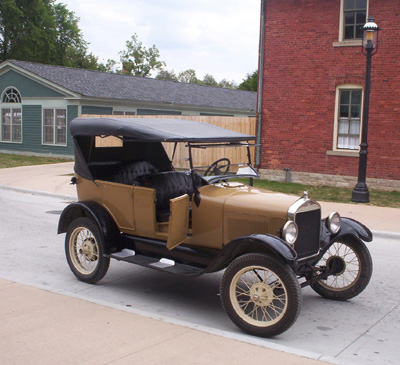
\includegraphics[width=.8\linewidth]{images/Late_model_Ford_Model_T.jpg}
  \caption{Ford modelo T del 1927 -- de Rmhermen \cite{Ford2022}.}
  \label{fig:ford_model_t}
\end{figure}

Durante aquella época, el ``mejor'' mecanismo de descubrimiento de
problemas era con algunos medidores y, sobre todo, por intuición:
sonidos del motor, olores extraños, \dots

No fue hasta los años 60 en donde los vehículos empezaron a incorporar
distintas interfaces con métricas que podían informar sobre el estado del
vehículo. El gran ``bum'' llegó con la expansión de la computadora, en donde
por primera vez se vio factible introducir un pequeño ordenador de 
abordo en el sistema.

En estos primeros sistemas, se incluyen indicadores del nivel de combustible,
sistema de refrigeración, presión del aceite, velocidad del motor,
temperatura del motor y otra información relativa al combustible. El
primer modelo que se conoce que incluye estos sistemas de cara a la
población en general es el Volkswagen Tipo III, en 1969 (figura \ref{fig:volkswagen_t3}):

\begin{figure}[H]
  \centering
  \includegraphics[width=.9\linewidth]{images/volkswagen_t3.jpg}
  \caption{Volkswagen Tipo III, modelo de inyección de 1969 -- de OSX - Trabajo propio \cite{VolkswagenTipo2021}.}
  \label{fig:volkswagen_t3}
\end{figure}

Pese a que supusieron un gran avance, estos primeros sistemas de
diagnóstico daban una información muy valiosa pero limitada, ya que muchos
diagnósticos seguirían siendo mediante los sentidos y las sensaciones
que le transmitiese el vehículo al mecánico. No fue hasta 1980 en donde
se implementó de forma estándar en los vehículos de \textit{General Motors}
el \ac{ALDL}, un lector de errores del coche que funcionó inicialmente a
160 baudios. Años más tarde, el sistema se refinaría usando el estándar
\ac{UART} \textit{half--duplex}, es decir, transmisión en los dos sentidos pero
no de forma simultánea (figura \ref{fig:aldl}). La principal motivación de incluir estos sistemas no fue
otra sino intentar reducir la contaminación de los vehículos teniendo
acceso a esta información \cite{SistemaOBD2Historia}.

\begin{figure}[H]
  \centering
  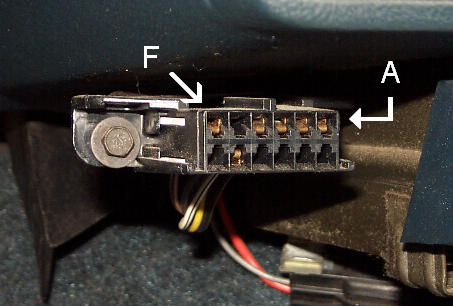
\includegraphics[width=.75\linewidth]{images/aldl.jpg}
  \caption{Conector \ac{ALDL}, creado por \textit{General Motors} antes de
  estandarizar OBD-II \cite{ReferenceManualChapter}.}
  \label{fig:aldl}
\end{figure}

No es hasta 1979 en que la \ac{SAE} recomienda crear un conector de
diagnóstico estandarizado en el mercado así como un conjunto de señales
de prueba. Finalmente, en 1991 la \ac{CARB} require que todos sus
vehículos tengan lo que sería el \ac{OBD}-I. Esta primera versión informaría
al conductor de un mal funcionamiento de alguno de los elementos del
vehículo mediante un \ac{MIL}, un indicador luminoso de fallos. Sin
embargo, solo se monitorizaban ciertos componentes relacionados con las
emisiones y no estaban calibrados \cite{SistemaOBD2Historia}.

Por ende, impulsado por las alertas \textit{smog} y por una fuerte regulación, en 1994
la \ac{CARB} obligó a todos los vehículos fabricados y vendidos a partir de 1996 incluir
el \ac{OBD}-II. Esto supuso un gran impulso en los mecanismos de monitorización de los
vehículos ya que además se estandarizó tanto el conector como los protocolos recomendados
por la \ac{SAE}. Tiempo más tarde, el Gobierno de los Estados Unidos aplicó la misma
medida a todos los vehículos del país \cite{SistemaOBD2Historia}.

Esta medida llegaría a Europa en 1998, según la Directiva 98/69EG, que obligaba a
todos los vehículos europeos a incluir dicho conector. Específicamente, los
automóviles de gasolina debían empezar a equiparlo en los modelos del año 2000; en el año 2003
para vehículos diésel; y en el año 2005 para camiones \cite{SistemaOBD2Historia}.

\subsection*{OBD--II}
\ac{OBD}--II es la segunda generación del sistema de diagnósticos de abordo, sucesor
de \ac{OBD}--I y su principal función es la de avisar al conductor cuando las
emisiones del vehículo son en torno a $1.5$ veces mayores de las diseñadas. A
diferencia de \ac{OBD}--I, \ac{OBD}--II también detecta fallos eléctricos, químicos
y mecánicos que puedan afectar al nivel de emisiones del vehículo (un caso típico
era un fallo químico del catalizador, indetectable por \ac{OBD}--I pero sí por la
segunda generación).

Este tipo de conector, al ser el primer estándar, cuenta con
múltiples interfaces que permiten conexiones mediante redes Wi-Fi, USB, Bluetooth,
etc. (cayendo pues en deshuso el protocolo de conexión por puerto serie -- RS232).
Esto se ha conseguido gracias al rápido avance de los sistemas embebidos, en donde
la combinación de \textit{software} y \textit{hardware} embebidos ha permitido que
cualquier usuario tenga acceso a este tipo de datos de forma relativamente simple
(actualmente, el conector más estandarizado es el controlador \texttt{ELM327} \cite{SistemaOBD2Historia},
figura \ref{fig:elm327}):

\begin{figure}[H]
  \centering
  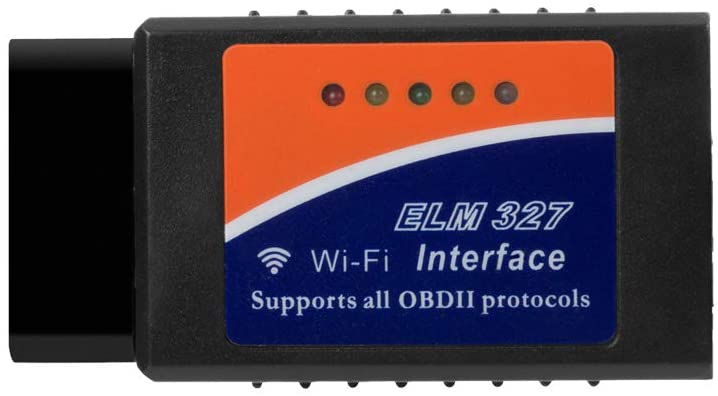
\includegraphics[width=.7\linewidth]{images/obd-ii-elm327.jpg}
  \caption{Controlador \texttt{ELM327} que cuenta con antenas Wi-Fi y Bluetooth para un acceso remoto \cite{AmazonComElm327}.}
  \label{fig:elm327}
\end{figure}

El sistema verifica todos los sensores directamente involucrados con las emisiones
del vehículo, como por ejemplo la inyección de aire al motor. Cuando algún sensor detecta
un fallo, se activa el \ac{MIL} indicando el fallo que sucede (o una combinación
de indicadores para notificar la existencia de un fallo, sin especificar exactamente
cuál).

El vehículo que incorpora un conector \ac{OBD}--II almacena la información sobre el
fallo del vehículo para que el mecánico que deba revisar el automóvil disponga de todos
los datos posibles. Por otra parte, este estándar permite una comunicación directa
con el vehículo mediante el envío de órdenes según un \ac{PID}. Por defecto, hay
una serie de \ac{PID}s estándar que la gran mayoría de vehículos deben incluir\footnote{%
Se dice ``la mayoría de vehículos'' porque hay ciertos \ac{PID}s que dependen
directamente del tipo de vehículo (a combustión, eléctrico, \dots) o del combustible
utilizado -- un vehículo eléctrico no ofrece información sobre las \ac{RPM} al igual
que un vehículo diésel no ofrece información sobre las bujías.}, pero también
los fabricantes de vehículos incluyen una serie de \ac{PID}s propios (conocidos como
\textit{\ac{PID}s propietarios}) que ofrecen información adaptada a cada vehículo
en particular y que, en principio, son privados y cerrados al público en general.

En Europa se implantó el \ac{EOBD}, la variación europea del estándar \ac{OBD}--II
implantada en el año 2000 en general. Si bien en apariencia es semejante al \ac{OBD}--II,
las diferencias radican en el \textit{software}. Por ejemplo, el estándar europeo
no monitoriza las evaporaciones del depósito de combustible; sin embargo, es más
sofisticado ya que usa ``mapas'' en las entradas de los sensores que obligan a que el
sensor se calibre empíricamente al sistema según las condiciones de operación del
motor (lo cual se traduce en que los sensores son mucho mejores pero más caros)
\cite{SistemaOBD2Historia}. Otra característica innovadora es que el sistema
europeo registra cuántos kilómetros se han recorrido desde que ha aparecido un
defecto \cite{EOBDOBD2}.

Finalmente, pero no menos importante, Japón tiene también su propio estándar denominado
\ac{JOBD}.

\subsection*{OBD--III}
El \ac{OBD}--III se espera que sea la siguiente versión del sistema que ya implementan
los coches actualmente. La principal diferencia con respecto a la versión anterior
será que el vehículo estará conectado de forma continua y emitiendo datos referentes
a las emisiones. De esta forma, se puede saber casi en el momento acerca de modificaciones
ilegales, un aumento en la contaminación del coche (signo de deterioro) y demás. No se
espera igualmente que sea un salto cualitativo ya que se sigue buscando que sea
altamente compatible con las herramientas que ya existen. Actualmente, se están
realizando pruebas en EE.UU. pero no hay cerrada ninguna fecha de estandarización
oficial por parte de los distintos continentes.

\subsection{Herramientas de monitorización y control del automóvil}
Pese al tiempo que lleva \ac{OBD}--II disponible, las herramientas existentes para
la actuación sobre un vehículo son relativamente escasas. La mayoría de modelos
presentes hoy en día en el mercado se basan directa o indirectamente en el
\texttt{ELM327}, un dispositivo de diagnóstico \ac{OBD} que cuenta con conexión
WiFi, Bluetooth y serie para la lectura local.

Por lo general, las herramientas que hay se utilizan por mecánicos o fanáticos del
sector para acceder a la información del estado del vehículo y ver los errores que
pudiera tener. Sin embargo, tras una breve documentación sobre el tema, la mayoría
de los casos buscaban directamente monitorizar en el momento el estado
del vehículo para obtener información relativa a los consumos, contaminación,
etc.

Por ejemplo, en el trabajo de Rimpas \textit{et al.} \cite{rimpasOBDIISensorDiagnostics2020}, se utiliza
un sensor \texttt{ELM327} para verificar que la información proporcionada por
el puerto del vehículo y la presentada por la telemetría presente en el mismo
(velocímetro y tacómetro) son coherentes entre sí (previa adaptación de los
valores en \textit{bytes} presentados por el conector a valores legibles). En
dicha investigación se llega a la conclusión de que el conector \ac{OBD}--II obtiene
valores fiables y consistentes tanto con los mostrados por el propio vehículo
como los proporcionados por el fabricante.

Otro tipo de investigaciones llevadas a cabo gracias a la presencia de este conector
en los automóviles es la de la caracterización de conductores y hábitos de conducción
según la telemetría reportada por el vehículo. En el estudio realizado por
Galih Hermawan y Emir Husni \cite{hermawanAcquisitionModelingEvaluating2020} se
estudia la combinación de la lectura de los sensores mediante el \ac{OBD}--II con
vehículos que presentan el sistema \ac{ADAS}.
El estudio busca identificar hábitos de conducción según la lectura de los diversos
sensores que hay en el sistema. También persigue detectar quién es el conductor que
está llevando el vehículo actualmente. En el estudio, el uso de \ac{OBD}--II junto
con los algoritmos de los \textit{k--Nearest Neighbor} (k--NN) y \textit{Naive Bayes}
consiguieron una precisión en la identificación del 100\% (
para un conjunto de datos de 10 conductores).
Por otra parte, el uso de inteligencia artificial junto con técnicas de \textit{clustering}
permitieron identificar comportamientos de los conductores al volante y relacionarlo
además con situaciones de riesgo y peligro. Además, se ha aplicado a otras características
también interesantes como detectar el tipo de calzada, predecir el tiempo de viaje,
analizar el consumo del vehículo y demás. El esquema seguido en la investigación es el
que se presenta en la figura \ref{fig:investigation-scheme}:

\begin{figure}[H]
  \centering
  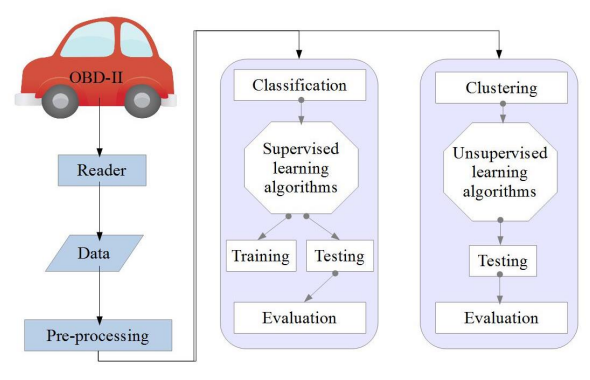
\includegraphics[width=.7\linewidth]{images/general-scheme-investigation.png}
  \caption{Esquema seguido para determinar los hábitos de conducción usando el \ac{OBD}--II \cite{hermawanAcquisitionModelingEvaluating2020}.}
  \label{fig:investigation-scheme}
\end{figure}

Por último, uno de los tipos de investigación bastante interesante realizada en los
últimos años es la de la generación de perfiles de conducción y de consumo. En el
artículo realizado por Ameen \textit{et al.} \cite{husseinaliameenDrivingBehaviourIdentification2021}
se define un sistema de clasificación del comportamiento del conductor al volante
(que es además el que se propone usar en este proyecto) el cual combina los datos
recibidos por el \ac{OBD}--II y del \ac{GPS} (figura \ref{fig:driving-behaviour}):

\begin{figure}[H]
  \centering
  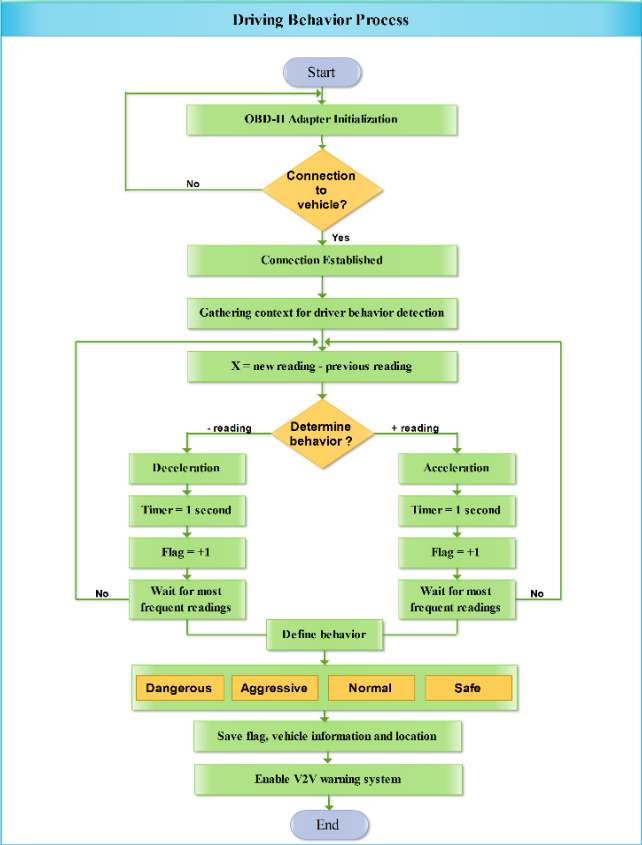
\includegraphics[width=.7\linewidth]{images/driving-behaviour-workflow.png}
  \caption{Flujo de análisis para determinar el comportamiento al volante de un conductor \cite{husseinaliameenDrivingBehaviourIdentification2021}.}
  \label{fig:driving-behaviour}
\end{figure}

Al final, el estudio concluía con los siguientes perfiles de conducción:

\begin{itemize}
  \item \textbf{Peligroso}, para una aceleración en general superior a $7\ \nicefrac{m}{s^2}$.
  \item \textbf{Agresivo}, para una aceleración entre $\left[4\ \nicefrac{m}{s^2}, 7\ \nicefrac{m}{s^2}\right)$.
  \item \textbf{Normal}, para una aceleración entre $\left[2\ \nicefrac{m}{s^2}, 4\ \nicefrac{m}{s^2}\right)$.
  \item \textbf{Seguro}, para una aceleración entre $\left[0\ \nicefrac{m}{s^2}, 2\ \nicefrac{m}{s^2}\right)$.
\end{itemize}

\section{Objetivos del desarrollo del proyecto}\label{sec:objectives}
Como se ha podido apreciar, existen multitud de aplicaciones relacionadas directa
o indirectamente con el \ac{OBD}--II, en parte por la longevidad del conector
en el mercado.

Sin embargo, todas o la gran mayoría de aplicaciones están destinadas a los profesionales
del sector, e incluso se ha aprovechado este conector para dificultar el acceso a
los datos del vehículo, habiendo de ir a un taller oficial para que puedan hacer
las reparaciones pertinentes.

Por otra parte, el parque de vehículos español es cada año más viejo debido a
diversos factores que no se van a analizar en este trabajo. Esto implica que cada
año más y más vehículos pierden el soporte por parte del fabricante y se vuelven
cada vez más costosos y complejos de mantener.

Para los no eruditos, el mundo del automóvil es el gran desconocido en donde una
serie de personas cualificadas se encargan del mantenimiento y correcto funcionamiento
del mecanismo que nos transporta por el mundo. Si bien es cierto que es necesaria
esta figura, hay una serie de buenas prácticas y actuaciones que pueden prevenir
tener que ir al mecánico de forma recurrente. Solo hace falta acceso a la información
de manera accesible.

Es por esto que nace \ac{VIMS}, un proyecto que pretende desarrollar un sistema completo
que consta de varias partes: un dispositivo embebido, un servidor y el usuario en sí
(figura \ref{fig:general-scheme}):

\begin{figure}[H]
  \centering
  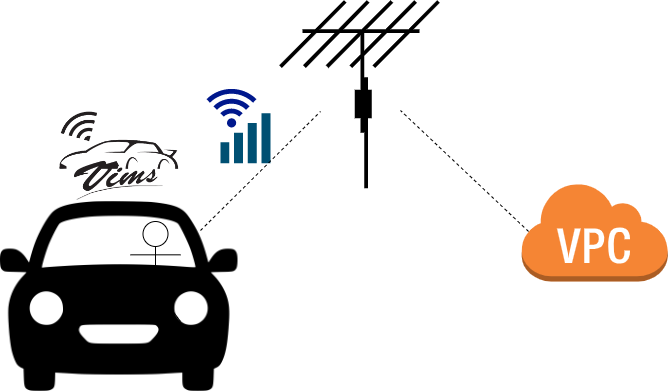
\includegraphics[width=\linewidth]{images/general-scheme.png}
  \caption{Esquema general que modela el modo de funcionamiento del sistema.}
  \label{fig:general-scheme}
\end{figure}

La idea fundamental detrás de este proyecto es la de devolverle a los usuarios
el control sobre su vehículo, ser conscientes de cómo funciona o, al menos, entender
mejor qué pueden hacer para mejorar tanto su estilo de conducción como la seguridad
al volante. De esta forma, con el dispositivo se espera también prevenir riesgos
ya que los propietarios y usuarios de los vehículos estarán informados en todo
momento de qué error pueda tener.

Como se prevé que este dispositivo sea utilizado por una gran variedad de usuarios
es crucial que sea accesible en términos de sencillez de manejo, entendimiento y
uso: evitar datos excesivamente técnicos, presentar la información más relevante
primero, etc.

Para ello, se hará uso de plataformas en la nube para gestionar, almacenar y presentar
la información al usuario y se contará con una aplicación móvil que permita un
fácil acceso a los datos del vehículo, tanto históricos como generados en el momento.

Al igual que otros trabajos previamente realizados, el proyecto se realiza sobre
las filosofías del código libre y del \textit{hardware} libre, que se traduce en
que todos los recursos (tanto físicos como \textit{software}) estarán disponibles
enteramente para cualquier persona interesada en ver cómo funciona, replicar el
proyecto por su cuenta y contar con plena potestad para mejorarlo, redistribuirlo
y trabajar con él (siempre bajo un prisma de reconocimiento al autor original
del trabajo regido por \textit{copyright}). Para ello, se ha decidido hacer uso
de la licencia MIT\footnote{Se pueden obtener más detalles sobre la licencia MIT
en la siguiente URL: \url{https://choosealicense.com/licenses/mit/}}.

\section{Metodología}\label{sec:methodology}
El proyecto que se pretende desarrollar es un proyecto de ingeniería. Esto se
traduce en que la metodología y la forma de trabajo son pilares fundamentales
en el desarrollo del mismo.

El primer paso realizado fue el de recopilar recursos e información de qué
necesitaban específicamente los usuarios. Para ello, se elaboró un cuestionario
en donde de forma general se preguntaba a conductores y no conductores qué querrían
tener en su vehículo. Los primeros sirvieron de grupo de control, los segundos para
aumentar la entropía de los datos obtenidos. El primer análisis realizado se detalla
en la sección \ref{ssec:user-req}, de la especificación de requisitos. Posteriormente,
en el punto \ref{chap:merch} se analiza en mayor profundidad los datos obtenidos
y se extraerán conclusiones.

A continuación, se realizó un estudio sobre qué plataformas y dispositivos están
accesibles de forma global para la generación y transmisión de datos. Esta fase
se centró principalmente en ``descubrir'' variantes del modelo ESP32 que incluyesen
ciertas antenas para permitir una mayor conectividad. Tras valorar diversas opciones,
se decidió usar el LILYGO T-SIM7000G ESP32 que incluye soporte de forma nativa para
tarjetas microSD, antena \ac{LTE}, alimentación externa por batería, antena \ac{GPS}, WiFi y
Bluetooth.

Una vez se decidió que dispositivo físico se iba a utilizar, se comenzó con el desarrollo
de los distintos diagramas que modelan el sistema, tanto lógicos como de diseño. Esta
parte fue crucial para asentar las bases de lo que será el proyecto y ha permitido seguir
el avance del mismo.

Por último, se realizó el serigrafiado de la placa y se comenzó la implementación
física de los diseños realizados. Sin embargo, esta etapa no se ha podido completar
por distintos contratiempos que se comentan en más detalle en el punto \ref{chap:planification}.


%% Product description
\chapter{Estructura del proyecto}\label{chap:structure}
El desarrollo del sistema \ac{VIMS} es un proceso multidisciplinar en el que se deben
desarrollar varias áreas de conocimiento. Este proyecto se ha postulado como
un desarrollo integral de ingeniería y es por eso por lo que está dividido en
varios bloques que conforman un factor clave en el desarrollo del mismo.

En este proyecto existen diversos bloques diferenciados: un estudio de mercado y de
las características de los usuarios, un estudio matemático asociado a la lectura de
valores y adecuación del \textit{hardware}, el proceso de diseño \textit{hardware}
en sí, el diseño \textit{software} del sistema y el análisis de planificación del mismo.

\begin{itemize}
  \item El estudio de mercado pretende averiguar y formalizar las necesidades de los
  conductores y usuarios de la vía. Es la primera aproximación y facilita la
  delimitación del producto y, sobre todo, ofrecerle al usuario final algo de utilidad
  y que pueda necesitar.
  \item El estudio matemático se encarga de investigar la ``traducción'' de los
  valores recibidos por el vehículo (según los datos asociados al estudio de mercado
  realizado con anterioridad).
  \item El diseño \textit{software} modela principalmente cómo se va a estructurar
  el sistema y cómo debe comportarse ante los distintos eventos que puede recibir.
  Esta fase conlleva realizar diagramas lógicos y de diseño del sistema en su conjunto.
  \item El diseño \textit{hardware} conlleva tanto el estudio de los componentes del
  sistema así como de las restricciones físicas del mismo. Además, en esta sección
  también se introduce el diseño 3D de la caja que alojará la placa.
  \item El análisis de planificabilidad complementa el diseño \textit{software}
  y estudia si el sistema es planificable. En los requisitos no se define \ac{VIMS}
  como un sistema en tiempo real, pero la cantidad de componentes que contiene y las
  acciones que tiene que realizar requieren del uso de subrutinas y de una planificación
  previa para asegurar un correcto funcionamiento del mismo.
\end{itemize}

Es importante detallar que pese a que el sistema se compone de varios componentes,
son dos los principales que lo caracterizan:

\begin{enumerate}
  \item La placa, \ac{VIMS}, que va embebida en los vehículos del sistema. Se encarga
  de toda la lectura, adaptación y emisión de datos. Además, cuenta con soporte para
  poder realizar una transmisión de la información a un dispositivo asociado mediante
  redes \ac{PAN}.
  \item El servidor \textit{cloud}, el ``cerebro'' encargado de recibir las tramas,
  los datos y la información relativa a las placas \ac{VIMS}, los dispositivos de
  usuario y demás componentes. Además, tiene la responsabilidad de ofrecer a los
  usuarios una \ac{GUI}, generar información relevante a partir de los datos (como
  estadísticas), gestionar las suscripciones y enviar periódicamente la información
  al usuario.
\end{enumerate}

\section{Estudio de mercado}\label{sec:merch}
Para el desarrollo de este proyecto, se hizo un estudio de mercado tanto de los
consumidores como de sus características, además de una evaluación exhaustiva
de qué les gustaría tener en su vehículo.

Este proyecto pretende en un futuro salir a mercado y suplir características que los
usuarios echan en falta en sus correspondientes medios de transporte. Como en principio
funciona con cualquier vehículo que cuente con \ac{OBD}--II, las respuestas no se han
limitado a aquellos conductores que condujesen turismos sino cualquier tipo de
automóvil: motocicleta, camión, etc.

Es importante destacar que el estudio tiene varios sesgos que han restringido
y delimitado las respuestas que se han registrado:

\begin{enumerate}
  \item Se ha realizado un cuestionario usando Google Forms, una plataforma de Google
        que permite preparar una serie de preguntas y respuestas y aplicar ciertos
        filtros sobre ellas. Por ejemplo, para aquellos que dijeron ser conductores,
        se hicieron preguntas diferentes frente a quienes no lo fueran.

        Esto permite obtener datos más fidedignos y acotados según la población que
        respondiera. Sin embargo, tiene una limitación implícita: restringe el acceso
        a aquellos con conocimientos ``suficientes'' acerca de la plataforma. Pese
        a que el producto pretende ser lo más accesible posible, no hay que olvidar
        que este tipo de tecnologías permanecen desconocidas para una gran parte
        de la población con escasos conocimientos acerca de Internet o de las
        nuevas tecnologías. Se comentará más adelante, pero esto se ve reflejado
        principalmente en la edad media de quienes respondieron el cuestionario.

        Por otra parte, al ser un cuestionario aparece otra limitación implícita
        y es la validación y verificación de las respuestas: se confía en la buena
        fe de los participantes y en la calidad de sus respuestas. Igualmente, se
        desarrolló el cuestionario junto con una psicóloga que ayudó a definir
        preguntas cerradas e incluir ciertas respuestas de control. Por otra parte,
        se usó el propio mecanismo que ofrece este servicio de Google para ordenar
        aleatoriamente las respuestas del cuestionario (y que eso sirviese también
        como control).

  \item Los encuestados fueron contactados principalmente por la red social Twitter,
        mediante la difusión con ``me gusta'' y ``retweet''. También se usaron otros
        medios de comunicación (como el correo UPM y Telegram/WhatsApp), pero el
        mayoritario fue el ya mencionado. Nuevamente, esto introduce un sesgo tanto
        por edad como por accesibilidad.

  \item Junto con la encuesta, se realizó un sorteo entre aquellos que respondiesen
        a la misma de un cheque regalo de Amazon valorado en 20\EUR{}. Si bien este
        incentivo pudiera resultar interesante, puede resultar también en un nuevo
        sesgo en donde personas que o bien no compren en Amazon o bien no sepan
        lo que es no quisieran hacer el cuestionario.

        Además, se plantea la casuística en que ciertas personas quisieran responder
        al cuestionario solo por el cheque de Amazon, sin importar la calidad de
        las respuestas, ``ensuciando'' los resultados obtenidos y quitándole credibilidad
        al cuestionario en sí.

        Esto se analizará posteriormente junto con las respuestas recibidas y las
        preguntas de control introducidas.

  \item El cuestionario, al ser relativamente exhaustivo, pudo echar para atrás a muchos
        posibles encuestados ya que se estima que el tiempo medio para realizarlo es del
        orden de 10/15 minutos. A parte del daño evidente de tener menos muestra con la
        que trabajar, este posible suceso reduciría también la variedad de la población
        y la calidad del estudio realizado.
\end{enumerate}

La primera pregunta que se realizó a los encuestados era si eran conductores o no.
Los datos revelan que el $72.7\%$ ($16$) de los encuestados son conductores, mientras que el
$27.3\%$ ($6$) restantes no, del total que fueron $22$ (figura \ref{fig:drivers-nodrivers}):

\begin{figure}[H]
  \centering
  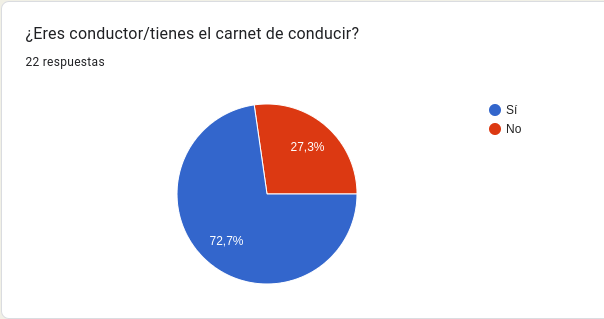
\includegraphics[width=\linewidth]{images/drivers-nodrivers.png}
  \caption{Gráfico de tarta que muestra quiénes de los encuestados son conductores ($72.7\%$) y quiénes no ($27.3\%$).}
  \label{fig:drivers-nodrivers}
\end{figure}

Sobre aquellos que dijeron ser conductores, se preguntó acerca de los años que
llevaban con carnet de conducir, así como los tipos de carnet de conducir que tenían
los encuestados.

Se vio que un $68.8\%$ tenía el carnet desde hace 3 años o más ($11$ encuestados
en particular); un $12.5\%$ tenía el carnet desde hace solo un año ($2$ encuestados)
y el restante, en su mayoría, tenía el carnet desde hace menos de un año. Esto se ve
reflejado en el histograma \ref{fig:carnet-time-hist}:

\begin{figure}[H]
  \centering
  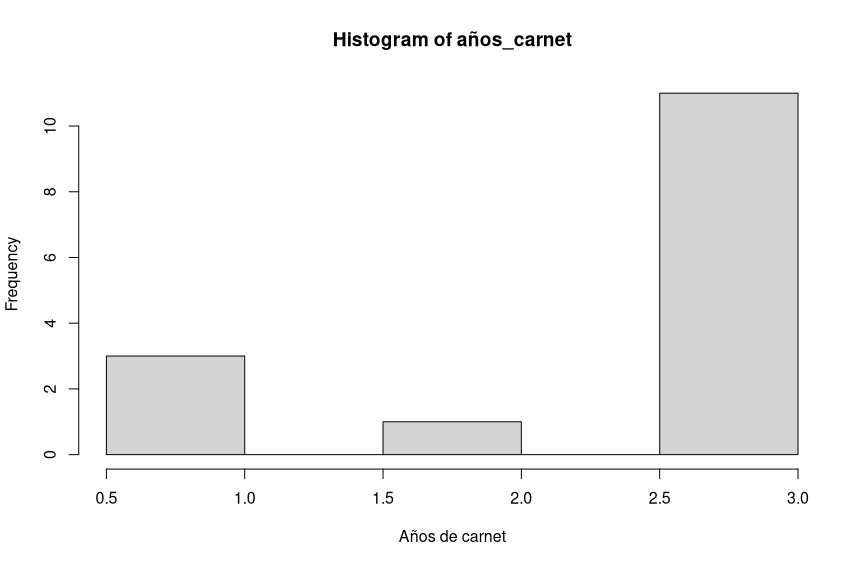
\includegraphics[width=\linewidth]{images/carnet-time.png}
  \caption{Histograma que muestra los años de carnet de los encuestados.}
  \label{fig:carnet-time-hist}
\end{figure}

Con respecto a los tipos de carnet, el $100\%$ de los encuestados (que dijeron ser
conductores) tiene el carnet tipo B. Se vio además que el $18.8\%$ tiene además los
carnets relativos a las motocicletas (muy posiblemente, los encuestados tienen el
carnet tipo ``A'' que les habilita automáticamente para aquellos de menor nivel,
como el AM, A1 y A2); y únicamente un encuestado tiene el carnet tipo C, que permite
conducir camiones.

Una restricción que se comentó con anterioridad era la edad media de los participantes.
Esta pregunta se realizó por dos motivos:

\begin{enumerate}
  \item Definir estadísticamente la edad media de la población para una posterior evaluación
        de su longevidad y experiencia tanto en la conducción como en la posible
        compra-venta de vehículos.
  \item Diferenciar, definir y clasificar los encuestados por grupos de edad y descubrir
        posibles sesgos y restricciones en las respuestas para un posterior análisis
        sobre la causa de dichos sesgos y restricciones.
\end{enumerate}

Es necesario decir que solo se preguntó por la edad a aquellas personas que respondieron
afirmativamente a ser conductores. Esto se hizo así debido a que sus respuestas han
conformado el dato más relativo a la hora de realizar la investigación, y se hace así
también estadísticamente.

Se tiene pues que:

\begin{equation}\label{eq:ages}
  \left\{\begin{aligned}
    X_{min}               & = 19     \\
    \bar{X}               & = 30     \\
    Mediana\left(X\right) & = 26.5   \\
    S\left(X\right)       & = 10.564 \\
    X_{max}               & = 55
  \end{aligned}\right.
\end{equation}

Se construyó además un gráfico de tarta (figura \ref{fig:ages}) que muestra cómo
quedan distribuidas las edades de los participantes:

\begin{figure}[H]
  \centering
  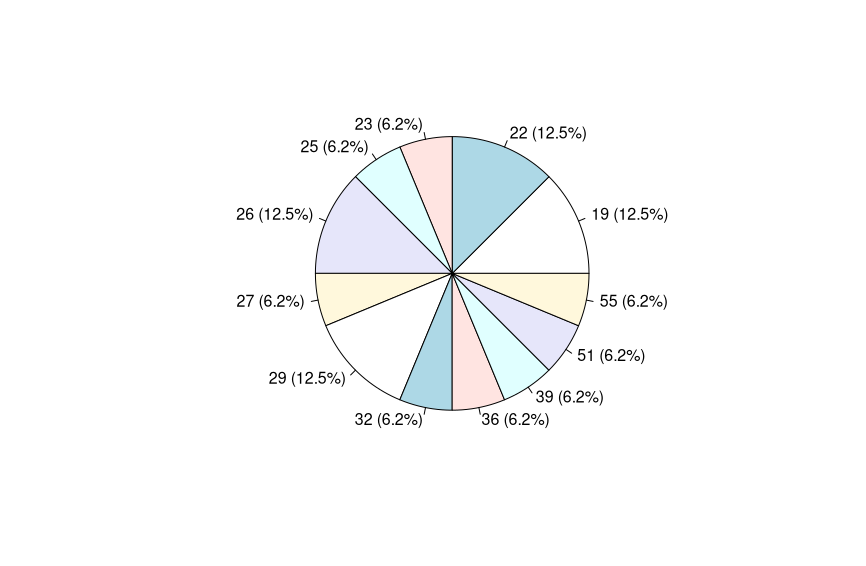
\includegraphics[width=\linewidth]{images/ages-pie.png}
  \caption{Gráfico de tarta que muestra la distribución de edades (valor previo al paréntesis) y su frecuencia en porcentaje.}
  \label{fig:ages}
\end{figure}

Como se puede ver en la ecuación \ref{eq:ages}, la distancia entre los valores
mínimo y máximo es de $36$ puntos. Sin embargo, los valores de la media $\left(\bar{X}\right)$
y la mediana $\left(Mediana\left(X\right)\right)$ muestran que la distribución está
bastante centrada en torno a la media, con una desviación estándar $\left(S\left(X\right)\right)$
de $\approx\pm10.564$.

Es interesante notar los tres grandes bloques presentes en la figura \ref{fig:ages}
que evidencian lo que se venía indicando anteriormente: en proporción, a la encuesta
ha accedido más población joven que adulta. Mismamente, solo el porcentaje de personas
encuestadas con edad por debajo de los 26 años es del $49.9\%$, casi la mitad de
los encuestados. Ampliando dicho margen hasta los 36 años, el porcentaje crece hasta
el $81 \%$.

Este dato se puede ver también reflejado en la distribución de los cuartiles, en donde
se tiene que:

\begin{equation}\label{eq:age-quartiles}
  \left\{
  \begin{aligned}
    Q_1 & = 22.75 \\
    Q_3 & = 33.00
  \end{aligned}
  \right.
\end{equation}

Como se puede apreciar en la ecuación \ref{eq:age-quartiles}, la distribución de
cuartiles está en un rango de edad por debajo de los 33 años para el $75\%$ de la
muestra, indicativo nuevamente de una población encuestada joven.

Destacan dos datos sobre los demás en donde los encuestados tienen 51 y 55 años
respectivamente. De este caso en particular se hablará posteriormente, pero cabe
destacar que sus respuestas fueron las más pobres en cuanto a contenido (sobre todo
en aquellas que sirvieron de control), seguramente debido al formato del
cuestionario, fatiga tras responder las secciones anteriores, etc.

Una vez se indagó acerca de la información que identifica a la muestra, se preguntó
directamente por el vehículo con el que contaban así como las características del
mismo. Para esta sección, se han dividido las preguntas en tres categorías:
\textit{básico}, \textit{habitual} y \textit{premium}. Dichas categorías se crean
según el porcentaje de uso habitual mundial de las características que se
enumeran en la tabla \ref{tab:car-specs}:

\begin{table}[H]
  \centering
  \begin{tabular}{|c|c|c|}
    \hline
    \textbf{Básico}          & \textbf{Habitual}            & \textit{\textbf{Premium}} \\
    \hline\hline
    Control de crucero       & Pantalla táctil              & Asistente virtual         \\
    Limitador de velocidad   & GPS                          & Aplicación móvil          \\
    Cámara de visión trasera & Detección de ángulos muertos & Cámara \textit{on-board}  \\
    Botón de arranque        & Android Auto                 &                           \\
    \hline
  \end{tabular}
  \caption{Tabla de distribución de las características de los vehículos, preguntado en el cuestionario.}
  \label{tab:car-specs}
\end{table}

Tras el cuestionario, las frecuencias obtenidas fueron:

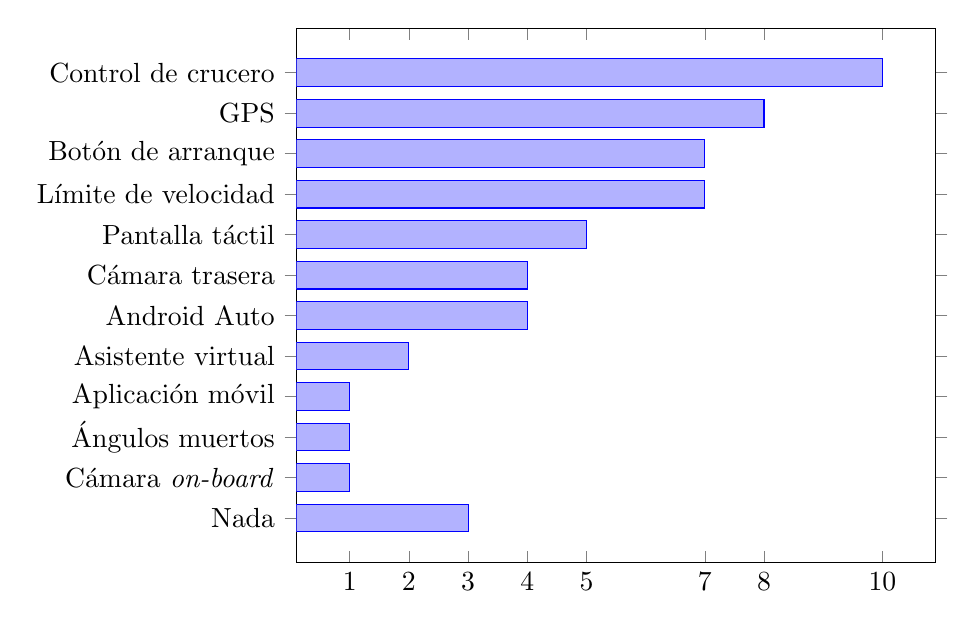
\begin{tikzpicture}
  \begin{axis} [%
      xbar,
      width=.8\linewidth,
      ytick=data,
      yticklabels={%
          Nada,
          Cámara \textit{on-board},
          Ángulos muertos,
          Aplicación móvil,
          Asistente virtual,
          Android Auto,
          Cámara trasera,
          Pantalla táctil,
          Límite de velocidad,
          Botón de arranque,
          GPS,
          Control de crucero,
        },
      xtick=data,
    ]
    \addplot coordinates {
        (3, 0)
        (1, 1)
        (1, 2)
        (1, 3)
        (2, 4)
        (4, 5)
        (4, 6)
        (5, 7)
        (7, 8)
        (7, 9)
        (8, 10)
        (10, 11)
      };
  \end{axis}
\end{tikzpicture}

\section{Estudio matemático}\label{sec:maths}
El estudio matemático va muy ligado al punto anterior (\ref{sec:merch}) ya que se
analizan los parámetros de \ac{OBD}--II y su ecuación matemática para obtener un
valor en $\mathbb{R}$ entendible por las personas.

Antes de dar paso a las ecuaciones en sí, es importante entender cómo funciona
el conector \ac{OBD}--II en esta situación. Los datos enviados y recibidos por
el coche están siempre codificados en un valor binario, recogido en un vector
de cuatro elementos en donde cada elemento tiene un \textit{byte} de tamaño. De
esta forma, se define al valor obtenido tras leer el conector \ac{OBD}--II como:

\begin{table}[H]
  \centering
  \resizebox{\textwidth}{!}{\begin{tabular}{|c|c|c|c|c|c|c|c|c|c|c|c|c|c|c|c|c|c|c|c|c|c|c|c|c|c|c|c|c|c|c|c|}
      \hline
      \multicolumn{8}{|c|}{$A$} & \multicolumn{8}{|c|}{$B$} & \multicolumn{8}{|c|}{$C$} & \multicolumn{8}{|c|}{$D$}                                                                                                                                                                                                                                 \\
      \hline
      $A_7$                     & $A_6$                     & $A_5$                     & $A_4$                     & $A_3$ & $A_2$ & $A_1$ & $A_0$ & $B_7$ & $B_6$ & $B_5$ & $B_4$ & $B_3$ & $B_2$ & $B_1$ & $B_0$ & $C_7$ & $C_6$ & $C_5$ & $C_4$ & $C_3$ & $C_2$ & $C_1$ & $C_0$ & $D_7$ & $D_6$ & $D_5$ & $D_4$ & $D_3$ & $D_2$ & $D_1$ & $D_0$ \\
      \hline
    \end{tabular}}
  \caption{Vector de \textit{bytes} que representa los datos recibidos del conector \ac{OBD}--II \cite{OBDIIPIDs2021}.}
  \label{tab:byte-array}
\end{table}

De esta forma, cuando se escribe $A_4$ se hace referencia al cuarto bit
del vector $A$. Los bits están ordenados según \ac{MSB}, de forma que
$A_7$ es el bit más significativo y $A_0$ el menor.

Los datos se obtienen del \ac{OBD}--II utilizando un lenguaje estándar llamado
\ac{PID}. El \ac{PID} se codifica como un número entero de 16 bits en donde los 8
primeros bits identifican el servicio/modo y los 8 restantes la operación a realizar.
Actualmente, están registrados los siguientes modos de funcionamiento (tabla
\ref{tab:pids-mode}):

\begin{table}[H]
  \centering
  \begin{tabularx}{\textwidth}{ | c | X | }
    \hline
    \textbf{Modo (hex)} & \textbf{Descripción}                                                                       \\
    \hline
    \texttt{01}         & Muestra los datos actuales del vehículo                                                    \\
    \hline
    \texttt{02}         & Muestra los datos almacenados del cuadro del vehículo                                      \\
    \hline
    \texttt{03}         & Muestra los códigos \ac{DTC}                                                               \\
    \hline
    \texttt{04}         & Elimina los códigos \ac{DTC} almacenados                                                   \\
    \hline
    \texttt{05}         & Resultados del test del sensor de oxígeno (sin \ac{CAN})                                   \\
    \hline
    \texttt{06}         & Resultados del test del sensor de oxígeno (con \ac{CAN})                                   \\
    \hline
    \texttt{07}         & Muestra los códigos \ac{DTC} pendientes (eliminados durante el último ciclo de conducción) \\
    \hline
    \texttt{08}         & Operaciones de control sobre los componentes del sistema                                   \\
    \hline
    \texttt{09}         & Petición de información sobre el vehículo                                                  \\
    \hline
    \texttt{0A}         & Códigos \ac{DTC} eliminados                                                                \\
    \hline
  \end{tabularx}
  \caption{Lista de modos de funcionamiento del estándar \ac{OBD}--II \cite{OBDIIPIDs2021}.}
  \label{tab:pids-mode}
\end{table}

Es importante destacar que no todos los fabricantes tienen por qué soportar todos
los modos, y que además ciertos fabricantes pueden definir sus modos propios por encima
del valor \texttt{09}.

Todos los modos definidos anteriormente tienen un conjunto de órdenes de soporte
en donde el sistema indica qué \ac{PID}s están soportados y cuáles no, por cada 32
\ac{PID}s. Por ejemplo, enviar la orden \texttt{0x0100} (\textit{modo 1, PID 0})
devolverá un valor que representará si los siguientes 32 \ac{PID}s están soportados.
Si el valor fuese, por ejemplo, \texttt{BE1FA813} se tendría que:

\begin{table}[H]
  \centering
  \resizebox{\textwidth}{!}{\begin{tabular}{ | c | c | c | c | c | c | c | c | c | c | c | c | c | c | c | c | c | c | c | c | c | c | c | c | c | c | c | c | c | c | c | c | c | }
      \hline
      \textbf{Hexadecimal} & \multicolumn{4}{|c|}{\texttt{B}} & \multicolumn{4}{|c|}{\texttt{E}} & \multicolumn{4}{|c|}{\texttt{1}} & \multicolumn{4}{|c|}{\texttt{F}} & \multicolumn{4}{|c|}{\texttt{A}} & \multicolumn{4}{|c|}{\texttt{8}} & \multicolumn{4}{|c|}{\texttt{1}} & \multicolumn{4}{|c|}{\texttt{3}}                                                                                                                                                                                                                                                                                                                                                 \\
      \hline
      \textbf{Binario}     & \texttt{1}                       & \texttt{0}                       & \texttt{1}                       & \texttt{1}                       & \texttt{1}                       & \texttt{1}                       & \texttt{1}                       & \texttt{0}                       & \texttt{0}  & \texttt{0}  & \texttt{0}  & \texttt{1}  & \texttt{1}  & \texttt{1}  & \texttt{1}  & \texttt{1}  & \texttt{1}  & \texttt{0}  & \texttt{1}  & \texttt{0}  & \texttt{1}  & \texttt{0}  & \texttt{0}  & \texttt{0}  & \texttt{0}  & \texttt{0}  & \texttt{0}  & \texttt{1}  & \texttt{0}  & \texttt{0}  & \texttt{1}  & \texttt{1}  \\
      \hline
      \textbf{?`Soportado?} & \done                            & \wontfix                         & \done                            & \done                            & \done                            & \done                            & \done                            & \wontfix                         & \wontfix    & \wontfix    & \wontfix    & \done       & \done       & \done       & \done       & \done       & \done       & \wontfix    & \done       & \wontfix    & \done       & \wontfix    & \wontfix    & \wontfix    & \wontfix    & \wontfix    & \wontfix    & \done       & \wontfix    & \wontfix    & \done       & \done       \\
      \hline
      \textbf{PID}         & \texttt{01}                      & \texttt{02}                      & \texttt{03}                      & \texttt{04}                      & \texttt{05}                      & \texttt{06}                      & \texttt{07}                      & \texttt{08}                      & \texttt{09} & \texttt{0A} & \texttt{0B} & \texttt{0C} & \texttt{0D} & \texttt{0E} & \texttt{0F} & \texttt{10} & \texttt{11} & \texttt{12} & \texttt{13} & \texttt{14} & \texttt{15} & \texttt{16} & \texttt{17} & \texttt{18} & \texttt{19} & \texttt{1A} & \texttt{1B} & \texttt{1C} & \texttt{1D} & \texttt{1E} & \texttt{1F} & \texttt{20} \\
      \hline
    \end{tabular}}
  \caption{Obtención de los \ac{PID}s soportados según el modo \cite{OBDIIPIDs2021}.}
  \label{tab:supported-pids}
\end{table}

A continuación, se dejan un conjunto de \ac{PID}s que se van a implementar en el
proyecto así como el código de acceso a ellos y la ecuación que permite obtener el
valor real.

\subsection*{Modo \texttt{01}}
Este modo permite acceder a la información en tiempo real del vehículo, según se
está en marcha. Los datos a los que se accede son:

\begin{table}[H]
  \centering
  \begin{tabularx}{\textwidth}{|c|X|}
    \hline
    \textbf{PID (hex)}       & \texttt{04}                    \\
    \hline
    \textbf{Bytes devueltos} & $1$                            \\
    \hline
    \textbf{Descripción}     & Carga del motor, en porcentaje \\
    \hline
    \textbf{Valor mínimo}    & $0\%$                          \\
    \hline
    \textbf{Valor máximo}    & $100\%$                        \\
    \hline
    \textbf{Fórmula}         &                                %
    \begin{equation*}
      \frac{A}{2.55}
    \end{equation*}                                 \\
    \hline
  \end{tabularx}
  \caption{\ac{PID} \texttt{04} -- carga del motor, en $\%$.}
\end{table}

\begin{table}[H]
  \centering
  \begin{tabularx}{\textwidth}{|c|X|}
    \hline
    \textbf{PID (hex)}       & \texttt{05}                            \\
    \hline
    \textbf{Bytes devueltos} & $1$                                    \\
    \hline
    \textbf{Descripción}     & Temperatura del refrigerante del motor \\
    \hline
    \textbf{Valor mínimo}    & $-40~\tccentigrade$                    \\
    \hline
    \textbf{Valor máximo}    & $215~\tccentigrade$                    \\
    \hline
    \textbf{Fórmula}         &                                        %
    \begin{equation*}
      A - 40
    \end{equation*}                                         \\
    \hline
  \end{tabularx}
  \caption{\ac{PID} \texttt{05} -- temperatura del refrigerante del motor, en $\tccentigrade$.}
\end{table}

\begin{table}[H]
  \centering
  \begin{tabularx}{\textwidth}{|c|X|}
    \hline
    \textbf{PID (hex)}       & \texttt{0C}         \\
    \hline
    \textbf{Bytes devueltos} & $2$                 \\
    \hline
    \textbf{Descripción}     & Velocidad del motor \\
    \hline
    \textbf{Valor mínimo}    & $0~RPM$             \\
    \hline
    \textbf{Valor máximo}    & $16383.75~RPM$      \\
    \hline
    \textbf{Fórmula}         &                     %
    \begin{equation*}
      \frac{256A + B}{4}
    \end{equation*}                      \\
    \hline
  \end{tabularx}
  \caption{\ac{PID} \texttt{0C} -- velocidad del motor, en $RPM$.}
\end{table}

\begin{table}[H]
  \centering
  \begin{tabularx}{\textwidth}{|c|X|}
    \hline
    \textbf{PID (hex)}       & \texttt{0D}            \\
    \hline
    \textbf{Bytes devueltos} & $1$                    \\
    \hline
    \textbf{Descripción}     & Velocidad del vehículo \\
    \hline
    \textbf{Valor mínimo}    & $0~\nicefrac{km}{h}$   \\
    \hline
    \textbf{Valor máximo}    & $255~\nicefrac{km}{h}$ \\
    \hline
    \textbf{Fórmula}         &                        %
    \begin{equation*}
      A
    \end{equation*}                         \\
    \hline
  \end{tabularx}
  \caption{\ac{PID} \texttt{0D} -- velocidad del vehículo, en $\nicefrac{km}{h}$.}
\end{table}

\begin{table}[H]
  \centering
  \begin{tabularx}{\textwidth}{|c|X|}
    \hline
    \textbf{PID (hex)}       & \texttt{11}             \\
    \hline
    \textbf{Bytes devueltos} & $1$                     \\
    \hline
    \textbf{Descripción}     & Posición del acelerador \\
    \hline
    \textbf{Valor mínimo}    & $0\%$                   \\
    \hline
    \textbf{Valor máximo}    & $100\%$                 \\
    \hline
    \textbf{Fórmula}         &                         %
    \begin{equation*}
      \frac{A}{2.55}
    \end{equation*}                          \\
    \hline
  \end{tabularx}
  \caption{\ac{PID} \texttt{11} -- posición del acelerador, en $\%$.}
\end{table}

\begin{table}[H]
  \centering
  \begin{tabularx}{\textwidth}{|c|X|}
    \hline
    \textbf{PID (hex)}       & \texttt{2F}                      \\
    \hline
    \textbf{Bytes devueltos} & $1$                              \\
    \hline
    \textbf{Descripción}     & Nivel del tanque del combustible \\
    \hline
    \textbf{Valor mínimo}    & $0\%$                            \\
    \hline
    \textbf{Valor máximo}    & $100\%$                          \\
    \hline
    \textbf{Fórmula}         &                                  %
    \begin{equation*}
      \frac{A}{2.55}
    \end{equation*}                                   \\
    \hline
  \end{tabularx}
  \caption{\ac{PID} \texttt{2F} -- nivel del tanque del combustible, en $\%$.}
\end{table}

\begin{table}[H]
  \centering
  \begin{tabularx}{\textwidth}{|c|X|}
    \hline
    \textbf{PID (hex)}       & \texttt{46}          \\
    \hline
    \textbf{Bytes devueltos} & $1$                  \\
    \hline
    \textbf{Descripción}     & Temperatura ambiente \\
    \hline
    \textbf{Valor mínimo}    & $-40~\tccentigrade$  \\
    \hline
    \textbf{Valor máximo}    & $215~\tccentigrade$  \\
    \hline
    \textbf{Fórmula}         &                      %
    \begin{equation*}
      A - 40
    \end{equation*}                      \\
    \hline
  \end{tabularx}
  \caption{\ac{PID} \texttt{46} -- temperatura ambiente, en $\tccentigrade$.}
\end{table}

\begin{table}[H]
  \centering
  \begin{tabularx}{\textwidth}{|c|X|}
    \hline
    \textbf{PID (hex)}       & \texttt{5B}                           \\
    \hline
    \textbf{Bytes devueltos} & $1$                                   \\
    \hline
    \textbf{Descripción}     & Tiempo restante de la batería híbrida \\
    \hline
    \textbf{Valor mínimo}    & $0\%$                                 \\
    \hline
    \textbf{Valor máximo}    & $100\%$                               \\
    \hline
    \textbf{Fórmula}         &                                       %
    \begin{equation*}
      \frac{A}{2.55}
    \end{equation*}                                       \\
    \hline
  \end{tabularx}
  \caption{\ac{PID} \texttt{5B} -- tiempo restante de la batería híbrida, en $\%$.}
\end{table}

\begin{table}[H]
  \centering
  \begin{tabularx}{\textwidth}{|c|X|}
    \hline
    \textbf{PID (hex)}       & \texttt{5C}            \\
    \hline
    \textbf{Bytes devueltos} & $1$                    \\
    \hline
    \textbf{Descripción}     & Temperatura del aceite \\
    \hline
    \textbf{Valor mínimo}    & $-40~\tccentigrade$    \\
    \hline
    \textbf{Valor máximo}    & $215~\tccentigrade$    \\
    \hline
    \textbf{Fórmula}         &                        %
    \begin{equation*}
      A - 40
    \end{equation*}                        \\
    \hline
  \end{tabularx}
  \caption{\ac{PID} \texttt{5C} -- temperatura del aceite, en $\tccentigrade$.}
\end{table}

\begin{table}[H]
  \centering
  \begin{tabularx}{\textwidth}{|c|X|}
    \hline
    \textbf{PID (hex)}       & \texttt{5E}               \\
    \hline
    \textbf{Bytes devueltos} & $2$                       \\
    \hline
    \textbf{Descripción}     & Consumo actual del motor  \\
    \hline
    \textbf{Valor mínimo}    & $0~\nicefrac{l}{h}$       \\
    \hline
    \textbf{Valor máximo}    & $3212.75~\nicefrac{l}{h}$ \\
    \hline
    \textbf{Fórmula}         &                           %
    \begin{equation*}
      \frac{256A + B}{20}
    \end{equation*}                           \\
    \hline
  \end{tabularx}
  \caption{\ac{PID} \texttt{5E} -- consumo actual del motor, en $\nicefrac{L}{h}$.}
\end{table}

\begin{table}[H]
  \centering
  \begin{tabularx}{\textwidth}{|c|X|}
    \hline
    \textbf{PID (hex)}       & \texttt{61}                       \\
    \hline
    \textbf{Bytes devueltos} & $1$                               \\
    \hline
    \textbf{Descripción}     & Torque demandado por el conductor \\
    \hline
    \textbf{Valor mínimo}    & $-125\%$                          \\
    \hline
    \textbf{Valor máximo}    & $130\%$                           \\
    \hline
    \textbf{Fórmula}         &                                   %
    \begin{equation*}
      A - 125
    \end{equation*}                                   \\
    \hline
  \end{tabularx}
  \caption{\ac{PID} \texttt{61} -- torque demandado por el conductor, en $\%$.}
\end{table}

\begin{table}[H]
  \centering
  \begin{tabularx}{\textwidth}{|c|X|}
    \hline
    \textbf{PID (hex)}       & \texttt{62}             \\
    \hline
    \textbf{Bytes devueltos} & $1$                     \\
    \hline
    \textbf{Descripción}     & Torque actual del motor \\
    \hline
    \textbf{Valor mínimo}    & $-125\%$                \\
    \hline
    \textbf{Valor máximo}    & $130\%$                 \\
    \hline
    \textbf{Fórmula}         &                         %
    \begin{equation*}
      A - 125
    \end{equation*}                         \\
    \hline
  \end{tabularx}
  \caption{\ac{PID} \texttt{62} -- torque actual del motor, en $\%$.}
\end{table}

\begin{table}[H]
  \centering
  \begin{tabularx}{\textwidth}{|c|X|}
    \hline
    \textbf{PID (hex)}       & \texttt{63}                    \\
    \hline
    \textbf{Bytes devueltos} & $2$                            \\
    \hline
    \textbf{Descripción}     & Torque de referencia del motor \\
    \hline
    \textbf{Valor mínimo}    & $0~Nm$                  \\
    \hline
    \textbf{Valor máximo}    & $65535~Nm$              \\
    \hline
    \textbf{Fórmula}         &                                %
    \begin{equation*}
      256A + B
    \end{equation*}                                \\
    \hline
  \end{tabularx}
  \caption{\ac{PID} \texttt{63} -- torque de referencia del motor, en $Nm$.}
\end{table}

\begin{table}[H]
  \centering
  \begin{tabularx}{\textwidth}{|c|X|}
    \hline
    \textbf{PID (hex)}       & \texttt{A4}                \\
    \hline
    \textbf{Bytes devueltos} & $4$                        \\
    \hline
    \textbf{Descripción}     & Marcha actual del vehículo \\
    \hline
    \textbf{Valor mínimo}    & $0~\text{ratio}$           \\
    \hline
    \textbf{Valor máximo}    & $65535~\text{ratio}$       \\
    \hline
    \textbf{Fórmula}         &                            %
    \begin{equation*}
      \begin{aligned}
        A_1 & = 1 \Longrightarrow \text{soportado} \\
        R   & = \frac{256C + D}{1000}
      \end{aligned}
    \end{equation*}                            \\
    \hline
  \end{tabularx}
  \caption{\ac{PID} \texttt{A4} -- marcha actual del vehículo, en ratio.}
\end{table}

\begin{table}[H]
  \centering
  \begin{tabularx}{\textwidth}{|c|X|}
    \hline
    \textbf{PID (hex)}       & \texttt{A6}      \\
    \hline
    \textbf{Bytes devueltos} & $4$              \\
    \hline
    \textbf{Descripción}     & Odómetro         \\
    \hline
    \textbf{Valor mínimo}    & $0~km$           \\
    \hline
    \textbf{Valor máximo}    & $429496729.5~km$ \\
    \hline
    \textbf{Fórmula}         &                  %
    \begin{equation*}
      \frac{A\left(2^{24}\right) + B\left(2^{16}\right) + C\left(2^8\right) + D}{10}
    \end{equation*}                  \\
    \hline
  \end{tabularx}
  \caption{\ac{PID} \texttt{A6} -- odómetro, en $km$.}
\end{table}

\subsection*{Modo \texttt{03}}
El modo \texttt{03} devuelve los \ac{DTC} guardados de la sesión actual. Estos códigos
de diagnóstico representan los distintos errores que hay en el vehículo, con un conjunto
de bytes que los identifican.

Este modo, a diferencia de los otros, no requiere de un parámetro \ac{PID} sino que solo
se envía el servicio como identificador. Una petición al modo \texttt{03} devolverá una
lista de $n$ elementos en donde cada elemento ocupa 2 bytes (por ende, el tamaño
esperable de la trama es $2n$).

Los códigos de error se definen como un conjunto de 5 caracteres de la forma: ``\texttt{U0158}''.
El valor de los caracteres define así:

\begin{table}[H]
  \centering
  \begin{minipage}{.32\linewidth}
    \begin{tabularx}{\textwidth}{|C{.3}|C{.7}|}
      \hline
      $A_7$ - $A_6$ & \textbf{Primer caracter \ac{DTC}}                         \\
      \hline
      \texttt{00}             & \textbf{P} -- sistema de propulsión (\textit{powertrain}) \\
      \texttt{01}             & \textbf{C} -- chassis                                     \\
      \texttt{10}             & \textbf{B} -- cuerpo (\textit{body})                      \\
      \texttt{11}             & \textbf{U} -- comunicaciones (\textit{network})           \\
      \hline
    \end{tabularx}
  \end{minipage}
  \hfill
  \begin{minipage}{.32\linewidth}
    \begin{tabularx}{\textwidth}{|C{.3}|C{.7}|}
      \hline
      $A_5$ - $A_4$ & \textbf{Segundo caracter \ac{DTC}} \\
      \hline
      \texttt{00}             & \texttt{0}                         \\
      \texttt{01}             & \texttt{1}                         \\
      \texttt{10}             & \texttt{2}                         \\
      \texttt{11}             & \texttt{3}                         \\
      \hline
    \end{tabularx}
  \end{minipage}
  \hfill
  \begin{minipage}{.32\linewidth}
    \begin{tabularx}{\textwidth}{|C{.3}|C{.7}|}
      \hline
      $A_3$ - $A_0$ & \textbf{Tercer caracter \ac{DTC}} \\
      \hline
      \texttt{0000}             & \texttt{0}                        \\
      \texttt{0001}             & \texttt{1}                        \\
      \texttt{0010}             & \texttt{2}                        \\
      \texttt{0011}             & \texttt{3}                        \\
      \texttt{0100}             & \texttt{4}                        \\
      \texttt{0101}             & \texttt{5}                        \\
      \texttt{0110}             & \texttt{6}                        \\
      \texttt{0111}             & \texttt{7}                        \\
      \texttt{1000}             & \texttt{8}                        \\
      \texttt{1001}             & \texttt{9}                        \\
      \texttt{1010}             & \texttt{A}                        \\
      \texttt{1011}             & \texttt{B}                        \\
      \texttt{1100}             & \texttt{C}                        \\
      \texttt{1101}             & \texttt{D}                        \\
      \texttt{1110}             & \texttt{E}                        \\
      \texttt{1111}             & \texttt{F}                        \\
      \hline
    \end{tabularx}
  \end{minipage}
\end{table}

Los caracteres cuarto y quinto se corresponden a los bits $B_7$ -- $B_4$ y $B_3$ -- $B_0$
respectivamente, y siguen la notación hexadecimal (al igual que los bits $A_3$ -- $A_0$).

De esta forma, con el código ya extraído, se necesita mirar en una tabla de valores
\ac{DTC} para saber exactamente a qué error se corresponde. Una web muy interesante
es la de ``OBD-Codes.com'' \cite{OBDCodesComLeading}, en donde hay información tanto
de códigos \ac{DTC} estándar como de códigos propietarios. Mirando en la propia
web, el código \texttt{U0158} se correspondería a: ``\textit{Lost communication with
head-up display}''\footnote{En la propia web dan muchos detalles e información
extendida sobre el error en cuestión, al igual que procedimientos para poder
solucionar el problema -- \url{https://www.obd-codes.com/u0158}}.

\subsection*{Modo \texttt{09}}
El modo \texttt{09} devuelve información referente al vehículo en sí, no al estado
de los sensores o del propio vehículo. Algunos datos interesantes son:

\begin{table}[H]
  \centering
  \begin{tabularx}{\textwidth}{|c|X|}
    \hline
    \textbf{PID (hex)}       & \texttt{02}                    \\
    \hline
    \textbf{Bytes devueltos} & $17$                            \\
    \hline
    \textbf{Descripción}     & \ac{VIN} \\
    \hline
    \textbf{Fórmula}         & \ac{VIN} de 17 caracteres ASCII con \textit{padding} a la izquierda de caracteres nulos (\texttt{0x00}) si hace falta \\
    \hline
  \end{tabularx}
  \caption{\ac{PID} \texttt{02} -- \ac{VIN}.}
\end{table}

\begin{table}[H]
  \centering
  \begin{tabularx}{\textwidth}{|c|X|}
    \hline
    \textbf{PID (hex)}       & \texttt{0A}                    \\
    \hline
    \textbf{Bytes devueltos} & $20$                            \\
    \hline
    \textbf{Descripción}     & Nombre de la \ac{ECU} \\
    \hline
    \textbf{Fórmula}         & 20 caracteres ASCII con \textit{padding} a la derecha de caracteres nulos (\texttt{0x00}) \\
    \hline
  \end{tabularx}
  \caption{\ac{PID} \texttt{0A} -- nombre de la \ac{ECU}.}
\end{table}

\section{Diseño \textit{software}}\label{sec:software}
\section{Diseño \textit{hardware}}\label{sec:hardware}
\section{Análisis de planificabilidad}\label{sec:rt-analysis}

%% Requirements
\chapter{Especificación de requisitos}\label{chap:requirements}
%% Introduction
\input{base/abstract.tex}

\chapter{Introducción}\label{chap:intro}
\input{content/introduction/introduction.tex}
\section{Estado del arte}\label{sec:state_of_the_art}
\input{content/introduction/state_of_the_art.tex}
\section{Objetivos del desarrollo del proyecto}\label{sec:objectives}
\input{content/introduction/objectives.tex}
\section{Metodología}\label{sec:methodology}
\input{content/introduction/methodology.tex}

%% Product description
\chapter{Estructura del proyecto}\label{chap:structure}
\input{content/description/structure.tex}
\section{Estudio de mercado}\label{sec:merch}
\input{content/description/merch.tex}
\section{Estudio matemático}\label{sec:maths}
\input{content/description/maths.tex}
\section{Diseño \textit{software}}\label{sec:software}
\section{Diseño \textit{hardware}}\label{sec:hardware}
\section{Análisis de planificabilidad}\label{sec:rt-analysis}

%% Requirements
\chapter{Especificación de requisitos}\label{chap:requirements}
\input{RS/content/content.tex}

%% Hardware and software design
\chapter{Diagramas y diseño}\label{chap:design}
\section{Diagramas que modelan el sistema}\label{sec:sys-diagrams}
\section{Diseño \textit{hardware} del sistema}\label{sec:hardware-design}
\section{Diseño 3D del sistema}\label{sec:3d-design}
\section{Diseño \textit{software} del sistema}\label{sec:software-design}
\section{Planificación del sistema de tiempo real}\label{sec:rt-design}

\chapter{Planificación, costes y tiempo empleado}\label{chap:planification}
\section{Diagramas de Gantt}
\section{Coste de los materiales}
\section{Sueldos propuestos y costes obtenidos}
\section{Contratiempos y tiempo de desarrollo final}

\chapter{Conclusiones}\label{chap:conclussions}
\section{Conclusiones técnicas}
\section{Conocimientos adquiridos y nuevas competencias}
\section{Reflexión final}

\chapter{Trabajo pendiente y futuras líneas de trabajo}\label{chap:pending-work}


%% Hardware and software design
\chapter{Diagramas y diseño}\label{chap:design}
\section{Diagramas que modelan el sistema}\label{sec:sys-diagrams}
\section{Diseño \textit{hardware} del sistema}\label{sec:hardware-design}
\section{Diseño 3D del sistema}\label{sec:3d-design}
\section{Diseño \textit{software} del sistema}\label{sec:software-design}
\section{Planificación del sistema de tiempo real}\label{sec:rt-design}

\chapter{Planificación, costes y tiempo empleado}\label{chap:planification}
\section{Diagramas de Gantt}
\section{Coste de los materiales}
\section{Sueldos propuestos y costes obtenidos}
\section{Contratiempos y tiempo de desarrollo final}

\chapter{Conclusiones}\label{chap:conclussions}
\section{Conclusiones técnicas}
\section{Conocimientos adquiridos y nuevas competencias}
\section{Reflexión final}

\chapter{Trabajo pendiente y futuras líneas de trabajo}\label{chap:pending-work}


%% Hardware and software design
\chapter{Diagramas y diseño}\label{chap:design}
\section{Diagramas que modelan el sistema}\label{sec:sys-diagrams}
\section{Diseño \textit{hardware} del sistema}\label{sec:hardware-design}
\section{Diseño 3D del sistema}\label{sec:3d-design}
\section{Diseño \textit{software} del sistema}\label{sec:software-design}
\section{Planificación del sistema de tiempo real}\label{sec:rt-design}

\chapter{Planificación, costes y tiempo empleado}\label{chap:planification}
\section{Diagramas de Gantt}
\section{Coste de los materiales}
\section{Sueldos propuestos y costes obtenidos}
\section{Contratiempos y tiempo de desarrollo final}

\chapter{Conclusiones}\label{chap:conclussions}
\section{Conclusiones técnicas}
\section{Conocimientos adquiridos y nuevas competencias}
\section{Reflexión final}

\chapter{Trabajo pendiente y futuras líneas de trabajo}\label{chap:pending-work}


%% Hardware and software design
\chapter{Diagramas y diseño}\label{chap:design}
En esta sección se detalla cómo se ha diseñado en general el sistema. Por una parte,
en la sección \ref{sec:sys-diagrams} se introducen los diagramas de casos de uso que dan
una visión general de cómo se va a organizar todo el sistema. Además, se comentan
también los diagramas de bloques que dan forma a la arquitectura final que se va
a implementar. A continuación, en la sección \ref{sec:hardware-design} se introduce
la PCB diseñada y las distintas decisiones de diseño que se han considerado a la hora
de la fabricación. Finalmente, en la sección \ref{sec:rt-design} se estructurarán
las tareas definidas en la sección \ref{sec:rt-analysis} y se realizará la
planificación en tiempo real del sistema.

\section{Diagramas que modelan el sistema}\label{sec:sys-diagrams}
Para facilitar el entendimiento del sistema al completo se han desarrollado dos
tipos de diagramas: los diagramas de casos de uso con sus correspondientes
explicaciones (punto \ref{ssec:use-case}) y los diagramas de bloques que modelan
al sistema en su conjunto, sus relaciones y operaciones (punto \ref{ssec:block-diagrams}).

Es importante destacar que los diagramas se quedan en una capa de abstracción por encima
de la definición de comportamiento del mismo, es decir, no se entra en excesivo detalle
sobre cómo va a hacer algo, solo especifica el qué.

\subsection{Casos de uso}\label{ssec:use-case}

A continuación se presentan los distintos diagramas de casos de uso que modelan el
comportamiento del sistema ante ciertos eventos. Se incluye además, por cada caso
de uso, una tabla adjunta que describe el caso de uso, los pasos esperados en la
secuencia normal de ejecución, las excepciones previstas durante la ejecución normal
y la resolución de las mismas.

\subsubsection{Caso de uso \texttt{01} -- autenticación}

\begin{figure}[H]
  \centering
  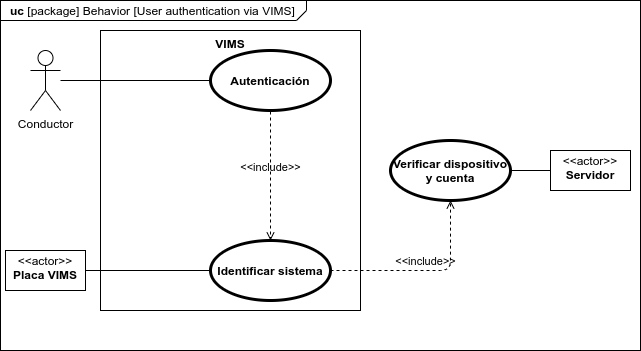
\includegraphics[width=\linewidth]{diagrams/UseCases-UC1 - auth.png}
  \caption{Caso de uso \texttt{01} -- \textit{autenticación}.}
  \label{uc:auth}
\end{figure}

\begin{table}[H]
  \centering
  \begin{tabularx}{\textwidth}{|c|c|X|}
    \hline
    \texttt{01}                                & \multicolumn{2}{c|}{\textit{Autenticación}}                                                                                                                                                                                                                 \\
    \hline
    \textbf{Descripción}                       & \multicolumn{2}{X|}{La placa identificará de forma inequívoca al conductor (usuario) y a sí misma frente al servidor.}                                                                                                                                      \\
    \hline
    \multirow{9}{*}{\textbf{Secuencia normal}} & \textbf{Paso}                                                                                                          & \textbf{Acción}                                                                                                                    \\
    \cline{2-3}
                                               & 1                                                                                                                      & \multicolumn{1}{L|}{El usuario se autentica contra la placa con su cuenta personal ya creada.}                                     \\
    \cline{2-3}
                                               & 2                                                                                                                      & \multicolumn{1}{L|}{La placa \ac{VIMS} recoge la información del usuario y la envía al servidor junto con su identificador único.} \\
    \cline{2-3}
                                               & 3                                                                                                                      & \multicolumn{1}{L|}{El servidor verifica que la cuenta del usuario existe y se asocia la información al dispositivo.}              \\
    \cline{2-3}
                                               & 4                                                                                                                      & \multicolumn{1}{L|}{La placa almacena la información del usuario y finaliza el proceso de inicio de sesión.}                       \\
    \hline
    \multirow{4}{*}{\textbf{Excepciones}}      & \textbf{Paso}                                                                                                          & \textbf{Acción}                                                                                                                    \\
    \cline{2-3}
                                               & 2                                                                                                                      & \multicolumn{1}{L|}{La placa no cuenta con conexión a la red o el servidor no está disponible.}                                    \\
    \cline{2-3}
                                               & 3                                                                                                                      & \multicolumn{1}{L|}{La cuenta del usuario no existe.}                                                                              \\
    \hline\hline
    \textbf{Resolución}                        & \multicolumn{2}{X|}{La placa funciona en modo desconectado, es decir, no transmite datos al servidor.}                                                                                                                                                      \\
    \hline
  \end{tabularx}
\end{table}

\subsubsection{Caso de uso \texttt{02} -- generación y transmisión de datos}

\begin{figure}[H]
  \centering
  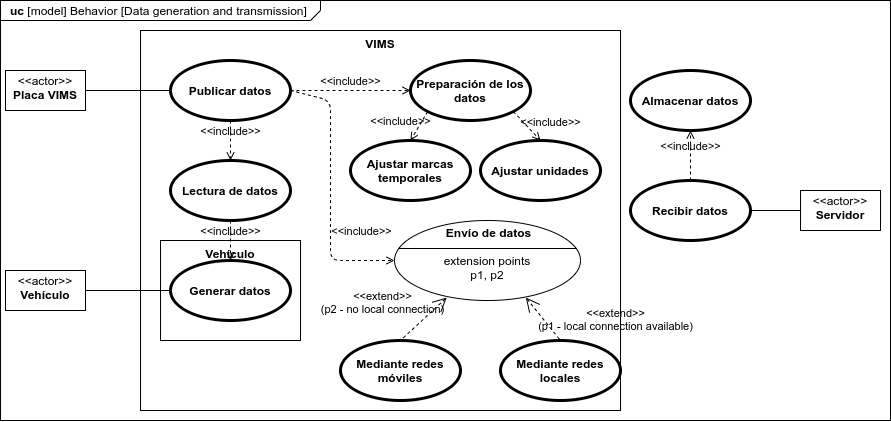
\includegraphics[width=\linewidth]{diagrams/UseCases-UC2 - data.png}
  \caption{Casos de uso \texttt{02} -- \textit{generación y transmisión de datos}.}
  \label{uc:data}
\end{figure}

\begin{table}[H]
  \centering
  \begin{tabularx}{\textwidth}{|c|c|X|}
    \hline
    \texttt{02}                                 & \multicolumn{2}{c|}{\textit{Generación y transmisión de datos}}                                                                                                                                                                                                                                                                                                                             \\
    \hline
    \textbf{Descripción}                        & \multicolumn{2}{X|}{El dispositivo \ac{VIMS} recibirá los datos del vehículo al que está conectado y los preparará para una posterior transmisión al servidor remoto de almacenamiento y gestión.}                                                                                                                                                                                          \\
    \hline
    \multirow{10}{*}{\textbf{Secuencia normal}} & \textbf{Paso}                                                                                                                                                                                                                & \textbf{Acción}                                                                                                                                              \\
    \cline{2-3}
                                                & 1                                                                                                                                                                                                                            & \multicolumn{1}{L|}{La placa \ac{VIMS} recibe los datos que el vehículo está generando de forma continuada.}                                                 \\
    \cline{2-3}
                                                & 2                                                                                                                                                                                                                            & \multicolumn{1}{L|}{Los datos recibidos se preparan para el envío, ajustando cierta información y añadiendo valores como la cuenta asociada a dichos datos.} \\
    \cline{2-3}
                                                & 3                                                                                                                                                                                                                            & \multicolumn{1}{L|}{Mediante el uso de redes móviles o locales, según disponibilidad, se envían los datos al servidor.}                                      \\
    \cline{2-3}
                                                & 4                                                                                                                                                                                                                            & \multicolumn{1}{L|}{El servidor recibe la información transmitida por el sistema y la almacena para una posterior visualización y tratamiento.}              \\
    \hline
    \multirow{9}{*}{\textbf{Excepciones}}       & \textbf{Paso}                                                                                                                                                                                                                & \textbf{Acción}                                                                                                                                              \\
    \cline{2-3}
                                                & 1                                                                                                                                                                                                                            & \multicolumn{1}{L|}{El vehículo no está conectado o no transmite datos.}                                                                                     \\
    \cline{2-3}
                                                & 2                                                                                                                                                                                                                            & \multicolumn{1}{L|}{Todavía no hay ninguna cuenta asociada a la placa \ac{VIMS}.}                                                                            \\
    \cline{2-3}
                                                & 3.1                                                                                                                                                                                                                          & \multicolumn{1}{L|}{No hay redes móviles disponibles, se intenta transmitir por redes locales.}                                                              \\
    \cline{2-3}
                                                & 3.2                                                                                                                                                                                                                          & \multicolumn{1}{L|}{No hay redes locales disponibles, se intenta transmitir por redes móviles.}                                                              \\
    \cline{2-3}
                                                & 3.3                                                                                                                                                                                                                          & \multicolumn{1}{L|}{No hay redes disponibles, se almacenan los datos para su posterior transmisión.}                                                         \\
    \hline\hline
    \textbf{Resolución}                         & \multicolumn{2}{X|}{La placa funciona en modo desconectado, es decir, no transmite datos al servidor. Si existe una cuenta asociada pero no hay conexión, los datos se almacenan en memoria hasta que se puedan transmitir.}                                                                                                                                                                \\
    \hline
  \end{tabularx}
\end{table}

\subsubsection{Caso de uso \texttt{03} -- generación de estadísticas}

\begin{figure}[H]
  \centering
  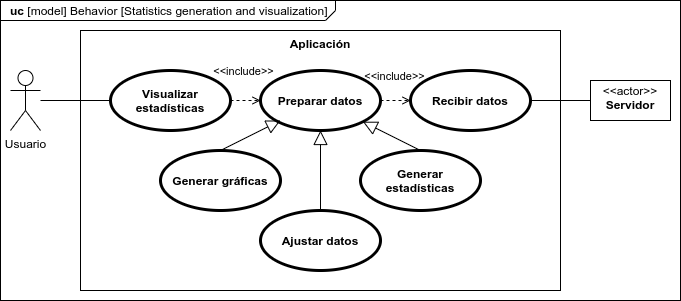
\includegraphics[width=\linewidth]{diagrams/UseCases-UC3 - stats.png}
  \caption{Caso de uso \texttt{03} -- \textit{generación de estadísticas}.}
  \label{uc:stats}
\end{figure}

\begin{table}[H]
  \centering
  \begin{tabularx}{\textwidth}{|c|c|X|}
    \hline
    \texttt{03}                                & \multicolumn{2}{c|}{\textit{Generación de estadísticas}}                                                                                                                                                                                                                                                                \\
    \hline
    \textbf{Descripción}                       & \multicolumn{2}{X|}{El servidor, en conjunción con el resto de elementos del sistema, preparará los datos para generar información estadística útil para el usuario.}                                                                                                                                                   \\
    \hline
    \multirow{7}{*}{\textbf{Secuencia normal}} & \textbf{Paso}                                                                                                                                                         & \textbf{Acción}                                                                                                                                 \\
    \cline{2-3}
                                               & 1                                                                                                                                                                     & \multicolumn{1}{L|}{El usuario solicita al servidor visualizar estadísticas con respecto a sus vehículos.}                                      \\
    \cline{2-3}
                                               & 2                                                                                                                                                                     & \multicolumn{1}{L|}{El servidor prepara los datos y genera distintos tipos de información estadística visual basados en tablas, gráficos, etc.} \\
    \cline{2-3}
                                               & 3                                                                                                                                                                     & \multicolumn{1}{L|}{El usuario recibe la información estadística ajustada a su cuenta.}                                                         \\
    \hline
    \multirow{4}{*}{\textbf{Excepciones}}      & \textbf{Paso}                                                                                                                                                         & \textbf{Acción}                                                                                                                                 \\
    \cline{2-3}
                                               & 1.1                                                                                                                                                                   & \multicolumn{1}{L|}{El usuario no está autenticado.}                                                                                            \\
    \cline{2-3}
                                               & 1.2                                                                                                                                                                   & \multicolumn{1}{L|}{El usuario no cuenta con ningún dispositivo \ac{VIMS} asociado.}                                                            \\
    \cline{2-3}
                                               & 2                                                                                                                                                                     & \multicolumn{1}{L|}{Todavía no se ha registrado ningún dato.}                                                                                   \\
    \hline\hline
    \textbf{Resolución}                        & \multicolumn{2}{X|}{Se notifica al usuario de este suceso y se le sugiere crear una cuenta.}                                                                                                                                                                                                                            \\
    \hline
  \end{tabularx}
\end{table}

\subsubsection{Caso de uso \texttt{04} -- envío de notificaciones}

\begin{figure}[H]
  \centering
  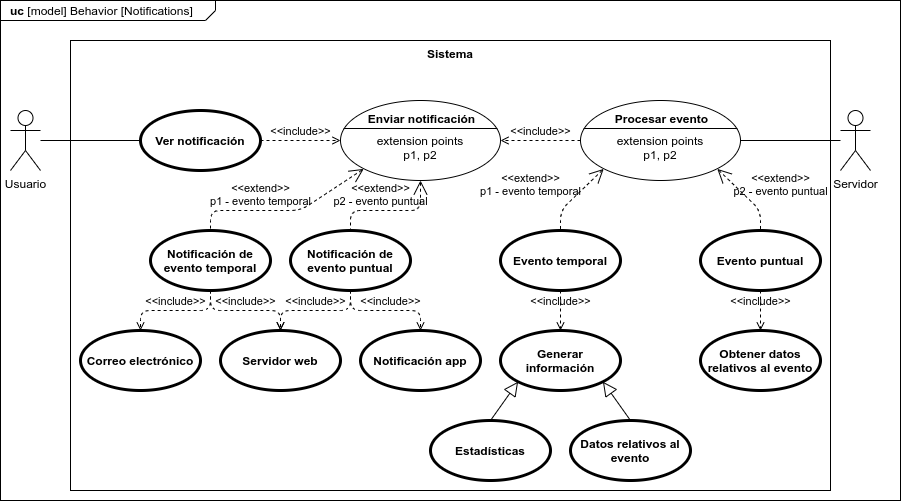
\includegraphics[width=\linewidth]{diagrams/UseCases-UC4 - notifications.png}
  \caption{Caso de uso \texttt{04} -- \textit{envío de notificaciones}.}
  \label{uc:notifications}
\end{figure}

\begin{table}[H]
  \centering
  \begin{tabularx}{\textwidth}{|c|c|X|}
    \hline
    \texttt{04}                                 & \multicolumn{2}{c|}{\textit{Envío de notificaciones}}                                                                                                                                                                                                                                                                                                                                                                                   \\
    \hline
    \textbf{Descripción}                        & \multicolumn{2}{X|}{El servidor, en conjunción con el resto de elementos del sistema, detecta ciertos eventos y actúa generando una notificación que envía al usuario.}                                                                                                                                                                                                                                                                 \\
    \hline
    \multirow{18}{*}{\textbf{Secuencia normal}} & \textbf{Paso}                                                                                                                                                           & \textbf{Acción}                                                                                                                                                                                                                                               \\
    \cline{2-3}
                                                & 1                                                                                                                                                                       & \multicolumn{1}{L|}{El servidor en un instante puntual produce y procesa un evento.}                                                                                                                                                                          \\
    \cline{2-3}
                                                & 1.1                                                                                                                                                                     & \multicolumn{1}{L|}{Si el evento se ha producido por un hecho (p.e.: repostar, finalizar un viaje, \dots), es un evento puntual sobre el cual se envía información relativa al mismo y al contexto (estadísticas del depósito, información del viaje, etc.).} \\
    \cline{2-3}
                                                & 1.2                                                                                                                                                                     & \multicolumn{1}{L|}{Si el evento se ha producido porque ha pasado un lapso de tiempo, es un evento temporal. El servidor generará estadísticas relativas a ese lapso de tiempo y mandará esa notificación.}                                                   \\
    \cline{2-3}
                                                & 2                                                                                                                                                                       & \multicolumn{1}{L|}{Se envía una notificación al usuario con los datos relativos al evento.}                                                                                                                                                                  \\
    \cline{2-3}
                                                & 2.1                                                                                                                                                                     & \multicolumn{1}{L|}{Si es un evento puntual, la notificación se envía a todos los medios: correo electrónico, servidor web y aplicación.}                                                                                                                     \\
    \cline{2-3}
                                                & 2.2                                                                                                                                                                     & \multicolumn{1}{L|}{Si es un evento temporal, la notificación se envía solo al correo electrónico y al servidor web.}                                                                                                                                         \\
    \cline{2-3}
                                                & 3                                                                                                                                                                       & \multicolumn{1}{L|}{El usuario recibe la notificación en alguno de los tres medios.}                                                                                                                                                                          \\
    \hline
  \end{tabularx}
\end{table}

\subsubsection{Caso de uso \texttt{05} -- visualización en tiempo real}

\begin{figure}[H]
  \centering
  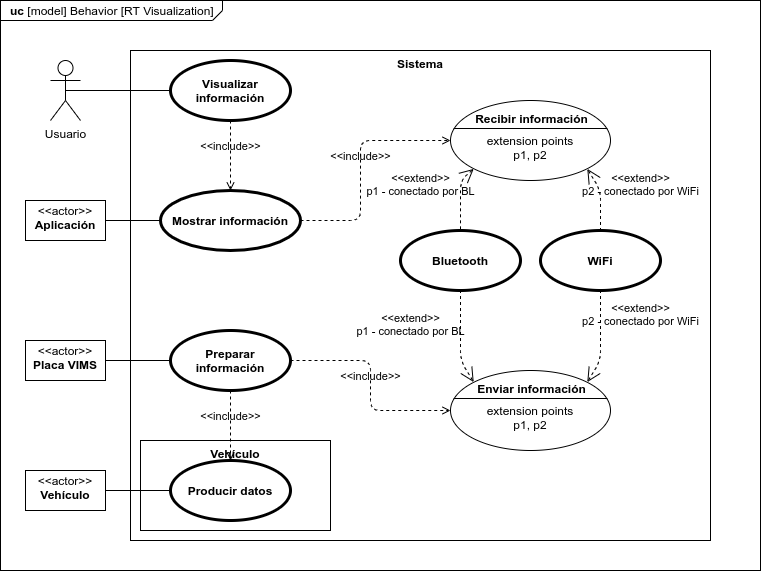
\includegraphics[width=\linewidth]{diagrams/UseCases-UC5 - visualization.png}
  \caption{Caso de uso \texttt{05} -- \textit{visualización en tiempo real}}
  \label{uc:visualization}
\end{figure}

\begin{table}[H]
  \centering
  \begin{tabularx}{\textwidth}{|c|c|X|}
    \hline
    \texttt{05}                                & \multicolumn{2}{c|}{\textit{Visualización en tiempo real}}                                                                                                                                                                                          \\
    \hline
    \textbf{Descripción}                       & \multicolumn{2}{X|}{Un usuario podrá visualizar información en tiempo real sobre su vehículo mediante la aplicación.}                                                                                                                               \\
    \hline
    \multirow{7}{*}{\textbf{Secuencia normal}} & \textbf{Paso}                                                                                                          & \textbf{Acción}                                                                                                            \\
    \cline{2-3}
                                               & 1                                                                                                                      & \multicolumn{1}{L|}{El usuario solicita visualizar información sobre el vehículo desde la aplicación.}                     \\
    \cline{2-3}
                                               & 2                                                                                                                      & \multicolumn{1}{L|}{La aplicación recibe la información de la placa \ac{VIMS} usando redes \ac{PAN}.}                      \\
    \cline{2-3}
                                               & 3                                                                                                                      & \multicolumn{1}{L|}{La placa \ac{VIMS} prepara la información que recibe del vehículo y la transmite hacia la aplicación.} \\
    \hline
    \multirow{10}{*}{\textbf{Excepciones}}     & \textbf{Paso}                                                                                                          & \textbf{Acción}                                                                                                            \\
    \cline{2-3}
                                               & 1.1                                                                                                                    & \multicolumn{1}{L|}{El usuario no está autenticado.}                                                                       \\
    \cline{2-3}
                                               & 1.2                                                                                                                    & \multicolumn{1}{L|}{El usuario no cuenta con ningún dispositivo \ac{VIMS} asociado.}                                       \\
    \cline{2-3}
                                               & 2.1                                                                                                                    & \multicolumn{1}{L|}{No hay conexión mediante Bluetooth, se realiza la comunicación por WiFi.}                              \\
    \cline{2-3}
                                               & 2.2                                                                                                                    & \multicolumn{1}{L|}{No hay conexión mediante WiFi, se realiza la comunicación por Bluetooth.}                              \\
    \cline{2-3}
                                               & 2.3                                                                                                                    & \multicolumn{1}{L|}{La placa \ac{VIMS} está desconectada.}                                                                 \\
    \cline{2-3}
                                               & 3                                                                                                                      & \multicolumn{1}{L|}{La placa \ac{VIMS} está desconectada o el vehículo no emite ningún dato.}                              \\
    \hline\hline
    \textbf{Resolución}                        & \multicolumn{2}{X|}{La placa no realiza ninguna transmisión de información hasta que no haya una conexión disponible.}                                                                                                                              \\
    \hline
  \end{tabularx}
\end{table}

\subsubsection{Caso de uso \texttt{06} -- generación de eventos}

\begin{figure}[H]
  \centering
  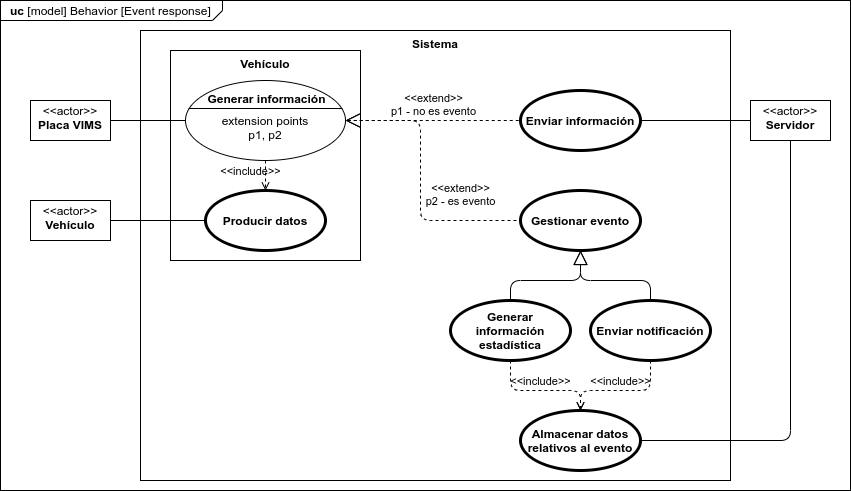
\includegraphics[width=\linewidth]{diagrams/UseCases-UC6 - reaction.png}
  \caption{Caso de uso \texttt{06} -- \textit{generación de eventos}}
  \label{uc:reaction}
\end{figure}

\begin{table}[H]
  \centering
  \begin{tabularx}{\textwidth}{|c|c|X|}
    \hline
    \texttt{06}                                 & \multicolumn{2}{c|}{\textit{Generación de eventos}}                                                                                                                                                                                                                                                                         \\
    \hline
    \textbf{Descripción}                        & \multicolumn{2}{X|}{El dispositivo \ac{VIMS}, a la hora de enviar datos, podrá producir eventos según el tipo de información que haya de enviar.}                                                                                                                                                                           \\
    \hline
    \multirow{10}{*}{\textbf{Secuencia normal}} & \textbf{Paso}                                                                                                                                     & \textbf{Acción}                                                                                                                                                         \\
    \cline{2-3}
                                                & 1                                                                                                                                                 & \multicolumn{1}{L|}{El dispositivo \ac{VIMS} genera información y la transmite hacia el servidor.}                                                                      \\
    \cline{2-3}
                                                & 1.1                                                                                                                                               & \multicolumn{1}{L|}{Si la información a transmitir es ``normal'', se envía directamente al servidor.}                                                                   \\
    \cline{2-3}
                                                & 1.2                                                                                                                                               & \multicolumn{1}{L|}{Si la información a transmitir es eventual, se procesa el evento generando información estadística referente al mismo o mandando una notificación.} \\
    \cline{2-3}
                                                & 2                                                                                                                                                 & \multicolumn{1}{L|}{El servidor recibe el evento y se encarga de gestionarlo, como se vio en el \texttt{UC-04}.}                                                        \\
    \hline
    \multirow{3}{*}{\textbf{Excepciones}}       & \textbf{Paso}                                                                                                                                     & \textbf{Acción}                                                                                                                                                         \\
    \cline{2-3}
                                                & 1                                                                                                                                                 & \multicolumn{1}{L|}{No hay ninguna cuenta asociada al dispositivo.}                                                                                                     \\
    \cline{2-3}
                                                & 1.1                                                                                                                                               & \multicolumn{1}{L|}{No hay conexión a Internet por parte del dispositivo \ac{VIMS}.}                                                                                    \\
    \hline\hline
    \textbf{Resolución}                         & \multicolumn{2}{X|}{La placa funciona en modo desconectado, es decir, no transmite datos al servidor.}                                                                                                                                                                                                                      \\
    \hline
  \end{tabularx}
\end{table}

\subsubsection{Caso de uso \texttt{07.*} -- envío, almacenamiento y visualización de geolocalización}

\begin{figure}[H]
  \centering
  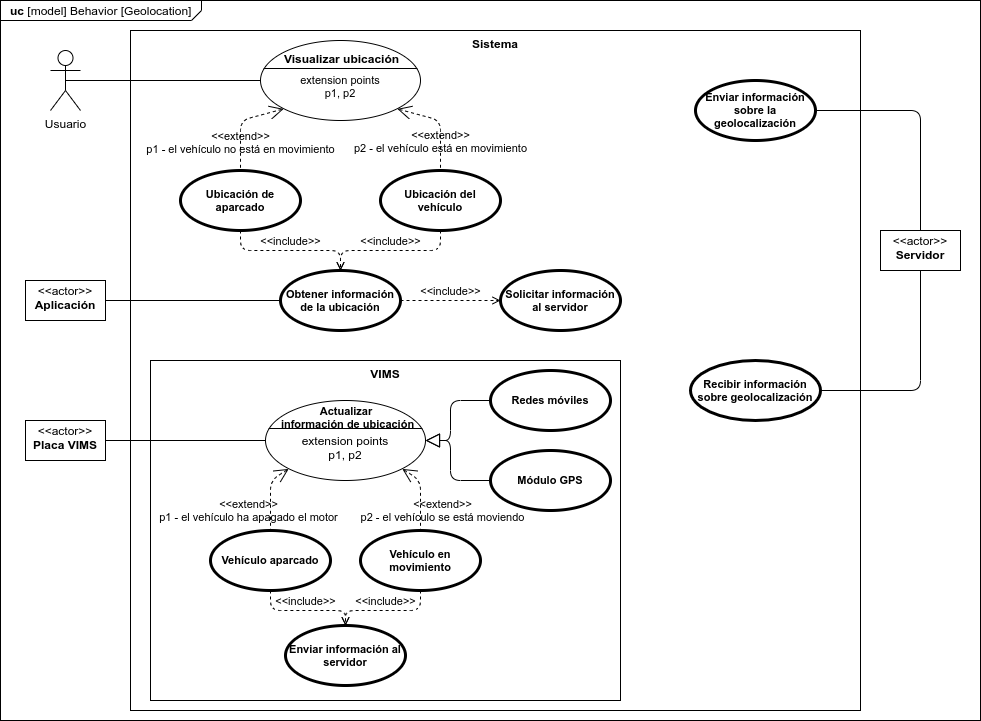
\includegraphics[width=\linewidth]{diagrams/UseCases-UC7 - location.png}
  \caption{Casos de uso \texttt{07.*} -- \textit{envío, almacenamiento y visualización de geolocalización}}
  \label{uc:location}
\end{figure}

\begin{table}[H]
  \centering
  \begin{tabularx}{\textwidth}{|c|c|X|}
    \hline
    \texttt{07.1}                               & \multicolumn{2}{c|}{\textit{Visualización de ubicación}}                                                                                                                                                                                                                                                                                                        \\
    \hline
    \textbf{Descripción}                        & \multicolumn{2}{X|}{El usuario mediante una aplicación podrá visualizar la ubicación del vehículo en tiempo real. Si el vehículo está apagado, se visualiza la ubicación del aparcamiento.}                                                                                                                                                                     \\
    \hline
    \multirow{10}{*}{\textbf{Secuencia normal}} & \textbf{Paso}                                                                                                                                                                               & \textbf{Acción}                                                                                                                                                   \\
    \cline{2-3}
                                                & 1                                                                                                                                                                                           & \multicolumn{1}{L|}{El usuario inicia una aplicación para visualizar la ubicación de su vehículo.}                                                                \\
    \cline{2-3}
                                                & 1.1                                                                                                                                                                                         & \multicolumn{1}{L|}{Si el vehículo se encuentra en movimiento, se visualiza la ubicación en tiempo real según se va actualizando.}                                \\
    \cline{2-3}
                                                & 1.2                                                                                                                                                                                         & \multicolumn{1}{L|}{Si el vehículo está apagado se considera que está aparcado y se visualiza la última ubicación conocida, correspondiente con el aparcamiento.} \\
    \cline{2-3}
                                                & 2                                                                                                                                                                                           & \multicolumn{1}{L|}{Se realizan peticiones al servidor para obtener la información de la geolocalización.}                                                        \\
    \hline
    \multirow{3}{*}{\textbf{Excepciones}}       & \textbf{Paso}                                                                                                                                                                               & \textbf{Acción}                                                                                                                                                   \\
    \cline{2-3}
                                                & 1                                                                                                                                                                                           & \multicolumn{1}{L|}{No hay ningún dispositivo asociado a la cuenta.}                                                                                              \\
    \cline{2-3}
                                                & 1.1                                                                                                                                                                                         & \multicolumn{1}{L|}{El vehículo está desconectado de la red, por lo que no se pueden transmitir los datos de geolocalización.}                                    \\
    \cline{2-3}
                                                & 1.2                                                                                                                                                                                         & \multicolumn{1}{L|}{No hay ningún dato de geolocalización almacenado.}                                                                                            \\
    \cline{2-3}
                                                & 2                                                                                                                                                                                           & \multicolumn{1}{L|}{La aplicación no cuenta con conexión a la red.}                                                                                               \\
    \hline\hline
    \textbf{Resolución}                         & \multicolumn{2}{X|}{La placa funciona en modo desconectado, es decir, no transmite datos al servidor.}                                                                                                                                                                                                                                                          \\
    \hline
  \end{tabularx}
\end{table}

\begin{table}[H]
  \centering
  \begin{tabularx}{\textwidth}{|c|c|X|}
    \hline
    \texttt{07.2}                               & \multicolumn{2}{c|}{\textit{Envío de ubicación}}                                                                                                                                                                                                                                                 \\
    \hline
    \textbf{Descripción}                        & \multicolumn{2}{X|}{La placa \ac{VIMS} enviará la información relativa al vehículo al servidor.}                                                                                                                                                                                                 \\
    \hline
    \multirow{18}{*}{\textbf{Secuencia normal}} & \textbf{Paso}                                                                                    & \textbf{Acción}                                                                                                                                                                               \\
    \cline{2-3}
                                                & 1                                                                                                & \multicolumn{1}{L|}{La placa actualiza la información sobre la ubicación del vehículo.}                                                                                                       \\
    \cline{2-3}
                                                & 1.1                                                                                              & \multicolumn{1}{L|}{Si se ha perdido la conexión con el vehículo (motor apagado), se considera que está aparcado y se envía la ubicación actual como ``ubicación de aparcado''.}              \\
    \cline{2-3}
                                                & 1.2                                                                                              & \multicolumn{1}{L|}{Si el vehículo está activo (motor encendido), se considera que está en movimiento y envía de forma periódica la ubicación actual del vehículo.}                           \\
    \cline{2-3}
                                                & 2                                                                                                & \multicolumn{1}{L|}{Según la precisión de las redes y la disponibilidad de las mismas, la ubicación se obtiene mediante dos métodos.}                                                         \\
    \cline{2-3}
                                                & 2.1                                                                                              & \multicolumn{1}{L|}{Se obtiene la ubicación mediante el uso de redes móviles cuando el módulo GPS no se encuentre disponible o no se tengan suficientes satélites.}                           \\
    \cline{2-3}
                                                & 2.2                                                                                              & \multicolumn{1}{L|}{Se obtiene la ubicación mediante el módulo GPS como primera alternativa, y se usan las redes móviles cuando estén disponibles para mejorar la precisión de la ubicación.} \\
    \cline{2-3}
                                                & 3                                                                                                & \multicolumn{1}{L|}{Se manda la ubicación obtenida al servidor y se enlaza a la cuenta asociada.}                                                                                             \\
    \hline
    \multirow{6}{*}{\textbf{Excepciones}}       & \textbf{Paso}                                                                                    & \textbf{Acción}                                                                                                                                                                               \\
    \cline{2-3}
                                                & 1                                                                                                & \multicolumn{1}{L|}{No hay ninguna cuenta asociada al dispositivo.}                                                                                                                           \\
    \cline{2-3}
                                                & 1.1                                                                                              & \multicolumn{1}{L|}{No hay ninguna conectividad de red disponible para realizar el envío de la ubicación.}                                                                                    \\
    \cline{2-3}
                                                & 3                                                                                                & \multicolumn{1}{L|}{La conexión de red no está disponible para realizar la transmisión de la información.}                                                                                    \\
    \hline\hline
    \textbf{Resolución}                        & \multicolumn{2}{X|}{La placa funciona en modo desconectado, es decir, no transmite datos al servidor.}                                                                                                                                                      \\
    \hline
  \end{tabularx}
\end{table}

\begin{table}[H]
  \centering
  \begin{tabularx}{\textwidth}{|c|c|X|}
    \hline
    \texttt{07.3}                              & \multicolumn{2}{c|}{\textit{Almacenamiento de los datos de ubicación}}                                                                                                                                                                                                        \\
    \hline
    \textbf{Descripción}                       & \multicolumn{2}{X|}{El servidor almacenará y gestionará los datos de ubicación recibidos por los múltiples dispositivos \ac{VIMS}.}                                                                                                                                           \\
    \hline
    \multirow{8}{*}{\textbf{Secuencia normal}} & \textbf{Paso}                                                                                                                       & \textbf{Acción}                                                                                                                         \\
    \cline{2-3}
                                               & 1                                                                                                                                   & \multicolumn{1}{L|}{El servidor recibe la información de la ubicación de un dispositivo \ac{VIMS}.}                                     \\
    \cline{2-3}
                                               & 1.1                                                                                                                                 & \multicolumn{1}{L|}{Los datos de ubicación se almacenan en una línea temporal para poder ver el histórico de ubicaciones del vehículo.} \\
    \cline{2-3}
                                               & 1.2                                                                                                                                 & \multicolumn{1}{L|}{El último valor de ubicación se almacena para una posterior visualización.}                                         \\
    \cline{2-3}
                                               & 2                                                                                                                                   & \multicolumn{1}{L|}{El servidor ofrece los datos de ubicación a través de la \ac{API}.}                                                 \\
    \hline
    \multirow{2}{*}{\textbf{Excepciones}}      & \textbf{Paso}                                                                                                                       & \textbf{Acción}                                                                                                                         \\
    \cline{2-3}
                                               & 1                                                                                                                                   & \multicolumn{1}{L|}{No hay ninguna cuenta asociada al dispositivo.}                                                                     \\
    \hline\hline
    \textbf{Resolución}                        & \multicolumn{2}{X|}{La placa funciona en modo desconectado, es decir, no transmite datos al servidor.}                                                                                                                                                      \\
    \hline
  \end{tabularx}
\end{table}

\subsection{Diagramas de bloques}\label{ssec:block-diagrams}

Los diagramas de bloques ofrecen una visión genérica del sistema en su conjunto. Para
este sistema, se han definido tres diagramas de bloques: el primero define a \textit{grosso modo}
cómo se compone el sistema embebido que irá en el vehículo, con sus respectivos
componentes y condiciones; el segundo, define la arquitectura del servidor, las conexiones
con la base de datos y la \ac{API} para consulta de datos externa. Finalmente, el
tercer diagrama muestra cómo es todo el sistema en su conjunto, uniendo \ac{VIMS}
con el servidor.

\begin{figure}[H]
  \centering
  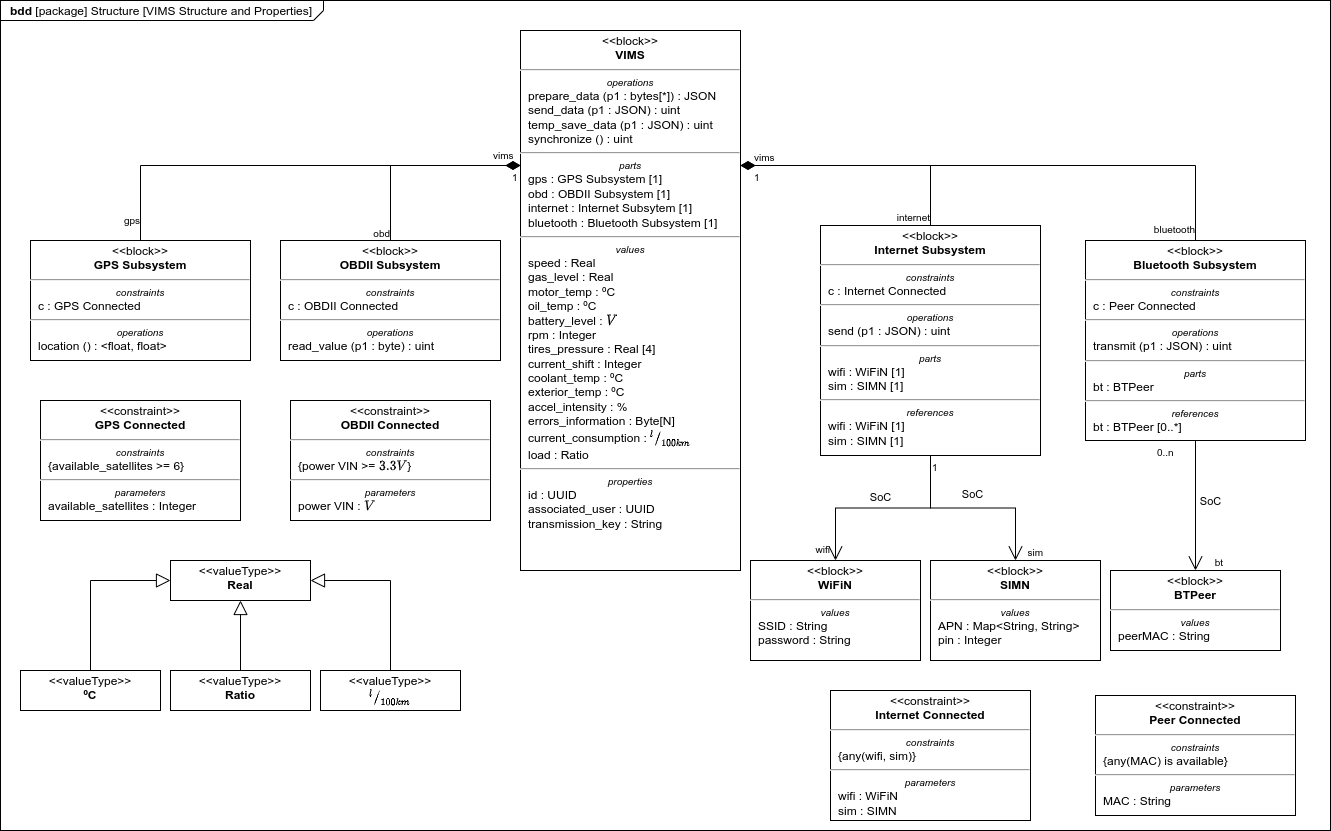
\includegraphics[width=\linewidth]{images/BlockDiagrams-VIMS.drawio.png}
  \caption{Diagrama de bloques que modela el conjunto de la placa \ac{VIMS} y sus componentes.}
  \label{bd:vims}
\end{figure}

Por una parte, se puede observar en la figura \ref{bd:vims} cómo está compuesta la placa.
Se distinguen los siguientes componentes principales:

\begin{itemize}
  \item El dispositivo \ac{VIMS} en sí, con sus funciones básicas y los datos que
        almacenará.
  \item El subsistema de conexionado \ac{GPS}, encargado de devolver la ubicación
        del sistema al que se conecta.
  \item El subsistema de conexionado \ac{OBD}--II, encargado de obtener en bytes
        los datos generados por el vehículo.
  \item El subsistema de conexionado a Internet, encargado de escoger adecuadamente
        el módulo de conexión a la red adecuado según las circunstancias del sistema
        y de realizar las comunicaciones de red.
  \item El subsistema de conexionado Bluetooth, cuya funcionalidad es la de conectarse
        a un dispositivo externo y realizar una emisión en el momento de los datos
        enviados por el vehículo.
\end{itemize}

Se va a empezar comentando cada uno de los subsistemas. Por su parte, el subsistema
\ac{GPS} (figura \ref{fig:bd-gps}) cuenta con una restricción ``\textit{GPS Connected}''
que define cuándo se considera que hay conexión con \ac{GPS}. Este valor se establece
en 6 satélites para resolver el problema del eje $Z$ que existe en trilateración con
3 satélites. En principio, con 4 satélites se podría considerar que hay conexión
con el \ac{GPS} pero con una redundancia del doble se obtiene una precisión de
aproximadamente $5~m$.

Este subsistema devuelve la latitud y la longitud, expresadas como números en coma
flotante de 32 bits (que dota al sistema de una precisión máxima de siete dígitos
decimales).

\begin{figure}[H]
  \centering
  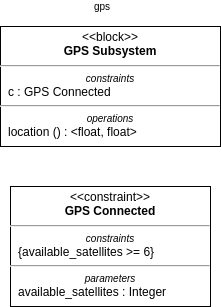
\includegraphics[width=.3\linewidth]{images/BD-GPS.png}
  \caption{Subsistema que define las comunicaciones usando el \ac{GPS} para obtener la ubicación.}
  \label{fig:bd-gps}
\end{figure}

El subsistema de \ac{OBD}--II (figura \ref{fig:bd-obd}) se encarga de la conexión con
el vehículo y remite los datos al sistema principal. La función \texttt{read\_value}
recibe un byte que se correspondería al \ac{PID} y devuelve los bytes con los datos
asociados. Al igual que el subsistema anterior, se plantea la restricción de que
el \ac{OBD}--II esté desconectado. Esto se hará confirmando que el $V_{in} \ge 3.3V$
aunque, en la vida real, esta restricción no existe dado que el sistema \ac{OBD}--II
del vehículo siempre está proveyendo de $12V$ al conector (sin embargo, se ha contemplado
porque existe la posibilidad de que la placa esté encendida mediante USB sin
conexión al vehículo).

\begin{figure}[H]
  \centering
  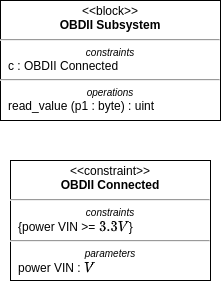
\includegraphics[width=.3\linewidth]{images/BD-OBD.png}
  \caption{Subsistema que define las comunicaciones con el vehículo usando \ac{OBD}--II.}
  \label{fig:bd-obd}
\end{figure}

El siguiente subsistema se encarga de la conectividad de red (figura \ref{fig:bd-internet}).
Contiene dos elementos ``\texttt{WiFiN}'' y ``\texttt{SIMN}'' en donde el primero
provee de conectividad WiFi y el segundo de conectividad \ac{LTE}. Este subsistema
cuenta con un único método que le permite enviar datos en forma JSON al exterior,
ya que es lo más compatible. Sin embargo, lo más importante es que se encarga de
escoger según disponibilidad un sistema u otro. Esto se realiza comprobando que
tienen acceso a la red según orden de prioridad: primero WiFi y luego SIM.

Individualmente, cada componente tiene las propiedades necesarias para conectarse.
Por su parte, la conexión WiFi contiene información sobre el SSID y la contraseña.
Mientras, la conexión \ac{LTE} (SIM) almacena los datos del APN y del pin de
desbloqueo de la SIM.

La restricción para que este subsistema se considere activo es que disponga de al
menos una conexión activa y funcional.

\begin{figure}[H]
  \centering
  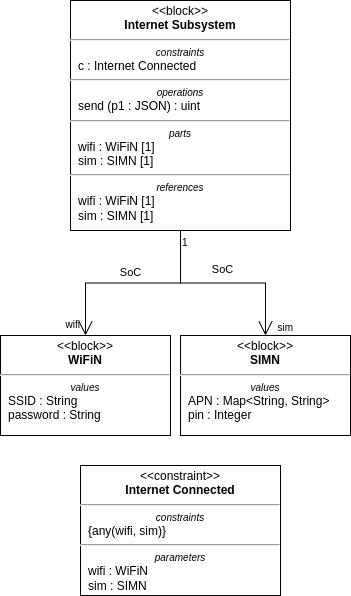
\includegraphics[width=.5\linewidth]{images/BD-Internet.png}
  \caption{Subsistema que define las comunicaciones de red con el exterior.}
  \label{fig:bd-internet}
\end{figure}

El último subsistema que forma parte de \ac{VIMS} es aquél que provee de conectividad
Bluetooth (figura \ref{fig:bd-bluetooth}). Este subsistema funciona en principio
usando \ac{BLE} por lo que es posible conectar múltiples dispositivos a la vez. Sin
embargo, por restricciones del proyecto se limita a una única conexión simultánea.
Por cada elemento emparejado, se almacena su dirección MAC para realizar la conexión
de nuevo.

Además, este subsistema tiene una restricción que define si está conectado si alguna
MAC almacenada está disponible y aceptando conexiones.

\begin{figure}[H]
  \centering
  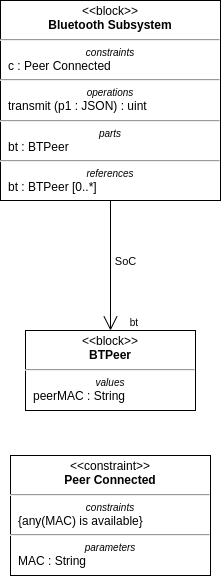
\includegraphics[width=.3\linewidth]{images/BD-Bluetooth.png}
  \caption{Subsistema de conexionado Bluetooth para la transmisión en vivo de los datos.}
  \label{fig:bd-bluetooth}
\end{figure}

Finalmente, queda el sistema principal: \ac{VIMS} que congrega al resto de subsistemas
y hace uso de las funcionalidades que ofrecen (figura \ref{fig:bd-vims}).

\begin{figure}[H]
  \centering
  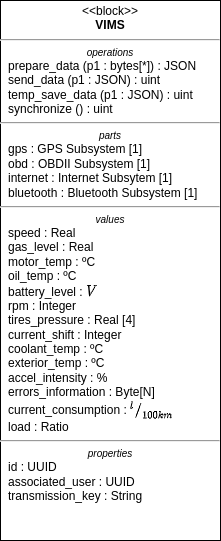
\includegraphics[width=.3\linewidth]{images/BD-VIMS.png}
  \caption{Componente \ac{VIMS} dentro del sistema embebido.}
  \label{fig:bd-vims}
\end{figure}

Este sistema se congrega de los subsistemas definidos anteriormente y define múltiples
métodos que realizan una serie de operaciones con los mismos. Por una parte, \texttt{prepare\_data}
prepara los valores recibidos en crudo por el subsistema \ac{OBD} para su posterior
transmisión. Esta operación realiza las conversiones adecuadas de los valores en
bytes, ajusta las unidades de los mismos y lo guarda en los campos correspondientes
definidos en ``\textit{values}''.

Por otra parte, la función \texttt{send\_data} envía los valores previamente preparados
al servidor remoto de gestión. El valor de retorno de esta operación es un código
entero que identifica la respuesta del servidor ante la transmisión.

Si por un casual el subsistema de conexión a Internet no se encuentra disponible
(es decir, no hay ni conexión WiFi ni SIM), existe la función \texttt{temp\_save\_data}
que almacenará los datos temporalmente en memoria persistente, hasta que se cuente
con conexión a la red.

Finalmente, existe la función \texttt{synchronize} que se encargará de mantener
actualizados los datos que se muestran en el dispositivo del usuario cuando dicho
dispositivo está conectado por Bluetooth y está en modo de monitorización.

En lo referente a los valores del bloque, se corresponden a los distintos datos que
serán accedidos usando el subsistema \ac{OBD} y que se guardan como referencia para
su posterior transmisión. No se va a entrar en detalle en explicar qué dato es cada
uno de los mostrados. Referirse a la sección \ref{sec:hardware} para más detalles.

Por último, en el apartado de propiedades, se almacenan todos aquellos valores
que identifican el dispositivo \ac{VIMS} en sí y la cuenta de usuario asociada
al mismo (junto con su clave de transmisión). Cada dispositivo \ac{VIMS} deberá
poder ser identificado de manera inequívoca y existe la posibilidad de que un mismo
usuario tenga múltiples dispositivos \ac{VIMS}. Como hay cierta información que
se puede considerar sensible, se genera una clave de transmisión asociada a la
cuenta y al dispositivo que permitirá asegurar la integridad, inmutabilidad y
confidencialidad de los datos durante la transmisión.

Estos valores se almacenan durante el primer arrancado del dispositivo. Según los
casos de uso (\ref{ssec:use-case}), el dispositivo \ac{VIMS} no hará nada mientras
esos campos no hayan sido cumplimentados, impidiendo cualquier operación con el
mismo.

\begin{figure}[H]
  \centering
  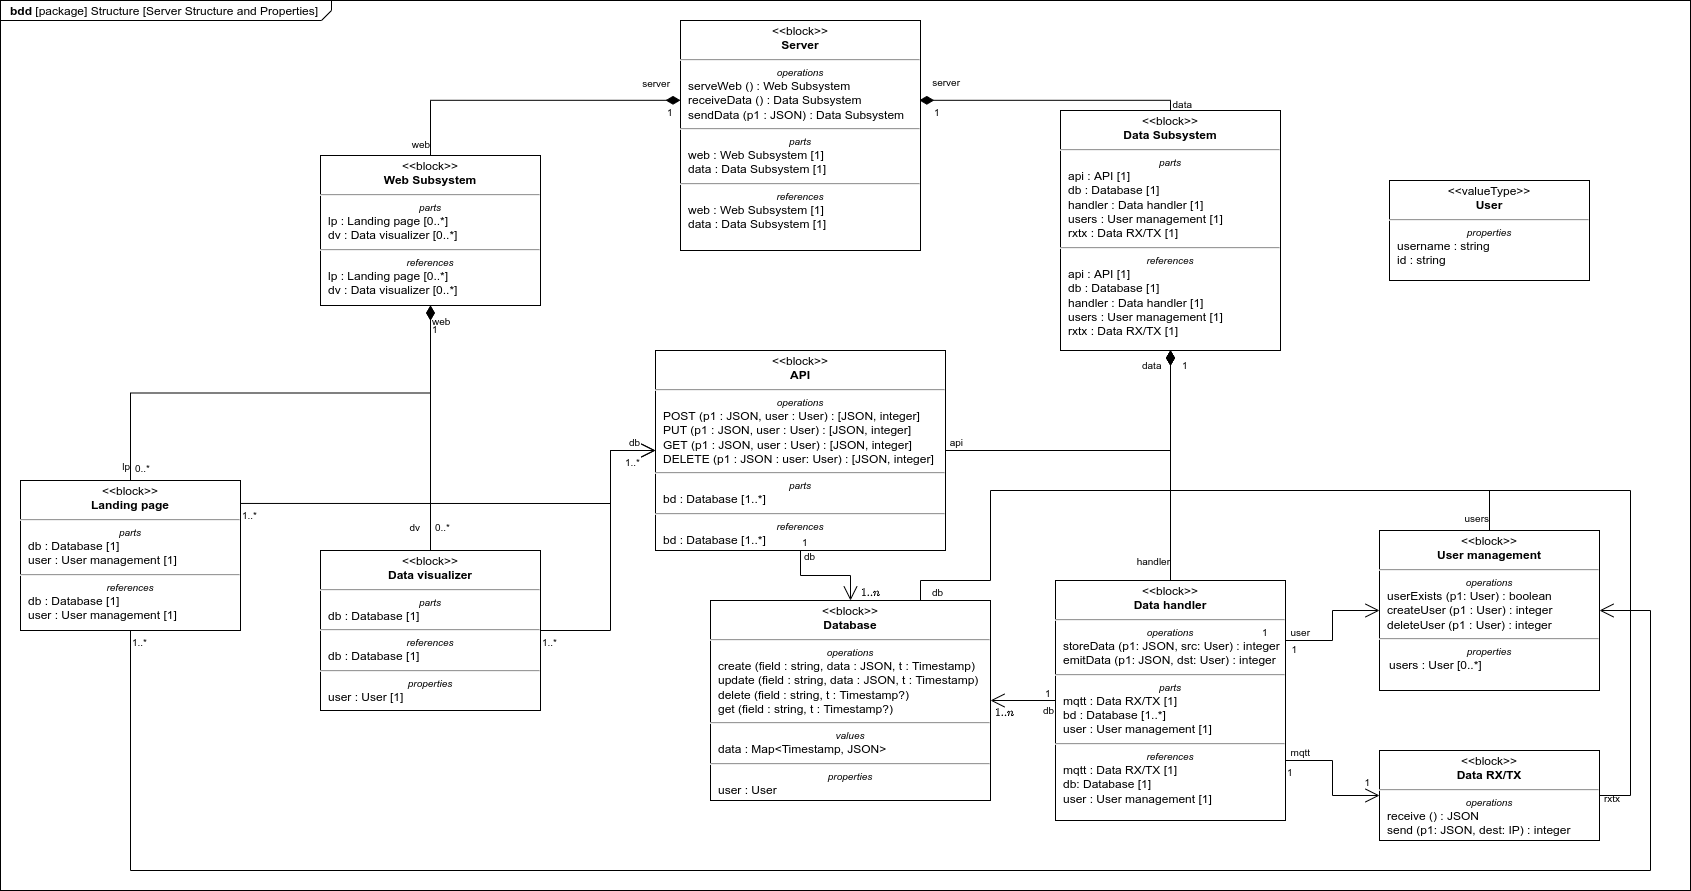
\includegraphics[width=\linewidth]{images/BlockDiagrams-Server.drawio.png}
  \caption{Diagrama de bloques que modela al servidor y sus componentes.}
  \label{bd:server}
\end{figure}

La arquitectura definida en el lado del servidor cuenta con menos componentes pero
más segregados:

\begin{itemize}
  \item El subsistema de la web, que define aquellos elementos que conforman la
        web con la que un usuario interactuará. Por una parte, existe una
        ``\textit{landing page}'' que permite que los usuarios se registren y
        creen sus cuentas. Por otro lado, se cuenta también con un visualizador
        de datos en donde el usuario podrá acceder a los últimos reportes
        sobre sus viajes y dispositivos, además de realizar las gestiones propias
        sobre su cuenta.
  \item El subsistema de datos, que engloba toda la gestión de la información
        por parte del servidor. Este subsistema se compone de una base de datos
        de almacenamiento de la información de usuario así como de los datos
        transmitidos por los dispositivos \ac{VIMS}. Otro bloque que lo conforma
        es el de gestión de la información el cual relacionará los datos recibidos
        por los dispositivos \ac{VIMS} con el usuario que los transmite. Finalmente,
        está el bloque de la \ac{API} que relaciona los dos subsistemas: accede a la
        información de manera segura almacenada en el bloque de los datos y se la
        ofrece al subsistema de la web y, en un futuro, al sistema de la aplicación
        móvil.
\end{itemize}

Toda esta arquitectura se ejecutará en un servicio en la nube que congregará y
simplificará las operaciones de mantenimiento y escalabilidad del sistema. Antes
de continuar, se va a analizar cada subsistema individualmente.

El subsistema de la web (figura \ref{fig:bd-web}) se compone de dos bloques principalmente:
un ``\textit{landing page}'' y un visualizador de datos. El primero de ellos, siguiendo
el flujo de operación definido en los casos de uso (\ref{ssec:use-case}), será
lo que un usuario arbitrario se encuentre cuando pretenda acceder al sistema por
primera vez. Allí, el usuario tendrá la capacidad de registrarse, almacenar sus
datos y registrar algún dispositivo \ac{VIMS}, si lo tiene. Como el servidor se
ejecuta en una nube alquilada, se plantea un modelo de suscripción libre en donde
un usuario puede decidir pagar una cuota mensual para acceder a las funcionalidades
del servidor.

Por otra parte, el visualizador de datos será la pantalla habitual que se encuentre un
usuario ya registrado. Allí se mostrará de forma agrupada y ordenada los datos
almacenados hasta el momento de los vehículos asociados a su cuenta (con una
estructura similar a la mostrada en la figura \ref{fig:data-ui}). Además del acceso
a los datos, el usuario podrá configurar sus preferencias, modalidad de suscripción,
dispositivos asociados, etc.

\begin{figure}[H]
  \centering
  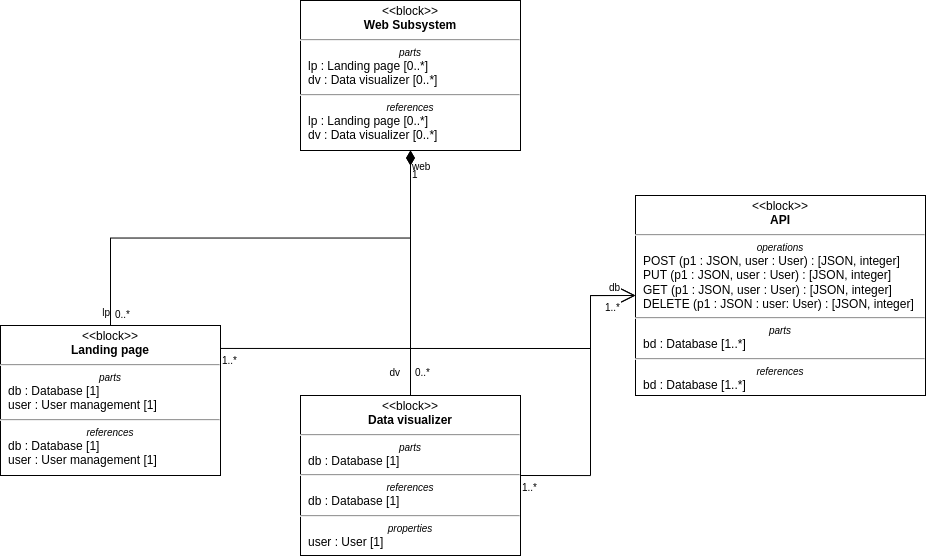
\includegraphics[width=.8\linewidth]{images/BD-web.png}
  \caption{Subsistema del servidor que conforma la arquitectura web del mismo.}
  \label{fig:bd-web}
\end{figure}

El subsistema de los datos (figura \ref{fig:bd-data}) cuenta con múltiples componentes
que lo conforman. El más básico de ellos que es usado por los demás es la base de datos.
Las operaciones definidas para dicha base de datos son \ac{CRUD}. La particularidad
de la base de datos es que cada ``instancia'' tiene asociada una cuenta de usuario,
de manera que las operaciones a realizar sobre la misma serán siempre con el usuario
como clave principal. Debido a los datos que se van a almacenar (que responden a
series temporales), el sistema propuesto de base de datos es una mezcla relacional y
no relacional. La primera se usará para almacenar toda la información que identifica
a los usuarios y sus características, que es un componente que está definido y es
limitado. Además, se almacenarán en esa base de datos toda aquella información
relacionada con las estadísticas del viaje, ya que es también una característica
inmutable. La segunda se usará para almacenar la información transmitida por los
dispositivos \ac{VIMS} dado que es una serie temporal. Se guardarán también datos
derivados de dicha transmisión y otra información de utilidad que pueda ser usada
posteriormente para generar perfiles de conducción, estadísticas, tendencias, etc.

Por otra parte, existe otro conjunto de bloques que representan las distintas
interacciones que puedan existir con los datos. Hay un bloque genérico llamado
``\textit{Data handler}'' que engloba las operaciones de escritura de los usuarios
y de los datos recibidos por los distintos dispositivos \ac{VIMS}. Este a su vez
se compone del bloque ``\textit{User management}'' que engloba las operaciones
de creación, lectura y eliminación de usuarios. El otro bloque es ``\textit{Data RX/TX}''
que se encarga de recibir los datos de los dispositivos \ac{VIMS} mediante el protocolo
MQTT. Además, también realizará las transmisiones hacia los dispositivos cuando
sea necesario (validar el usuario, actualizaciones de \textit{firmware}, \dots).

Finalmente, se encuentra el bloque de la \ac{API}. En particular, es una \ac{API} \ac{REST}
que permite realizar diversas operaciones sobre los datos asociados a una cuenta de
usuario. Al usar un sistema ampliamente estandarizado permite la interacción
directa de diversos sistemas como son \ac{VIMS}, el servidor en sí y la aplicación
móvil.

\begin{figure}[H]
  \centering
  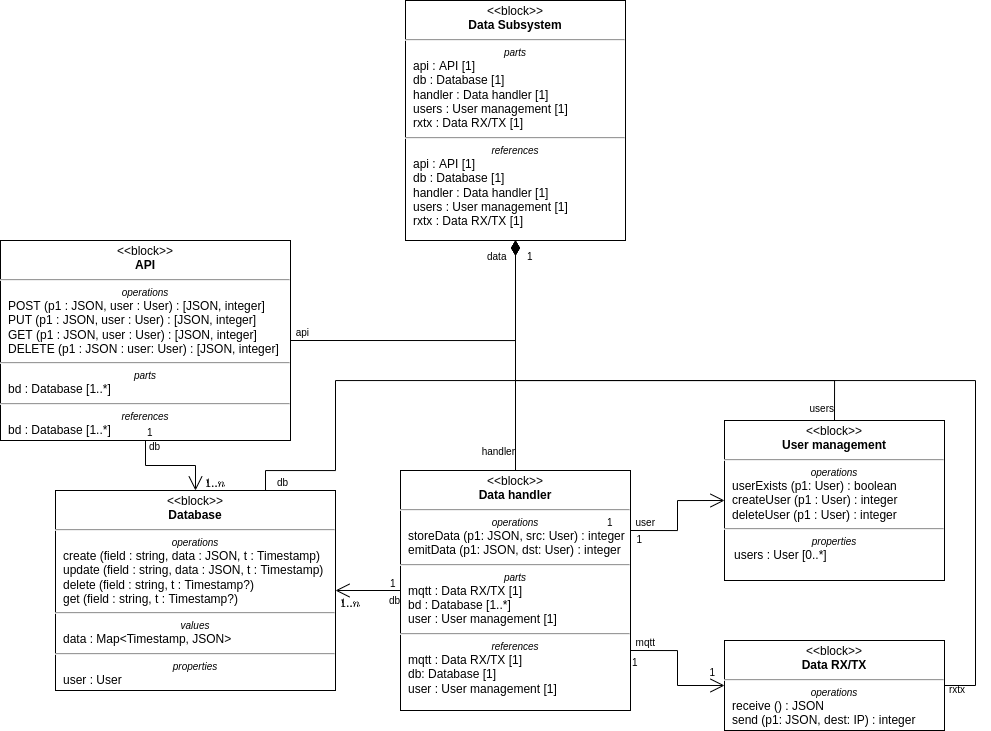
\includegraphics[width=\linewidth]{images/BD-data.png}
  \caption{Subsistema del servidor que conforma la gestión de datos y usuarios.}
  \label{fig:bd-data}
\end{figure}

Por último, se cuenta con un último diagrama que relaciona cómo funcionan los dos
esquemas de bloques anteriores (figura \ref{bd:global}):

\begin{figure}[H]
  \centering
  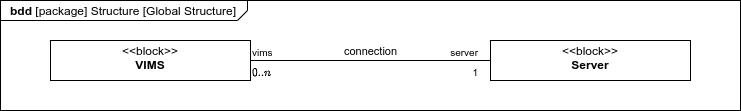
\includegraphics[width=\linewidth]{images/BlockDiagrams-Global.drawio.png}
  \caption{Diagrama global del sistema. Como se puede ver, se sigue una arquitectura cliente--servidor.}
  \label{bd:global}
\end{figure}

Como se puede observar, la multiplicidad contempla que hayan múltiples sistemas
\ac{VIMS} conectados y funcionando contra un único servidor (indiferentemente de
que, por razones de escalabilidad, este esté distribuido).

\section{Diseño \textit{hardware} del sistema}\label{sec:hardware-design}
El diseño \textit{hardware} es otro de los componentes clave de este proyecto. En esta
sección se hablará en particular de qué decisiones se han tomado a la hora de montar
el \textit{hardware}, cómo se han configurado y demás.

Por otra parte, se detallará el tipo de placa que se ha utilizado y qué características
tiene de partida que permiten facilitar el desarrollo del proyecto.

Finalmente, se incluyen detalles de cómo es el proceso de manufacturación de la PCB
así como de imágenes que muestran el resultado final.

\subsection{Selección de la placa}
Antes de desarrollar el \textit{hardware} o siquiera materializar la idea, se dedicó
un tiempo de investigación a ver qué había en el mercado que pudiese servir para
el propósito de este proyecto. Se consideraron los siguientes dispositivos (tabla
\ref{tab:devices}):


\begin{landscape}
  \begin{table}[H]
    \centering
    \begin{tabularx}{\linewidth}{|c|P{.11}|P{.2}|P{.25}|P{.44}|}
      \hline
      \textbf{\#} & \textbf{Nombre}                                                              & \textbf{Enlace de compra}                                  & \textbf{Enlace a repositorio}                                & \textbf{Comentarios}                           \\
      \hline
      1           & LILYGO\textsuperscript{\textregistered} TTGO T-SIM7000G                      & \url{https://es.aliexpress.com/item/4000542688096.html}    & \url{https://github.com/Xinyuan-LilyGO/LilyGO-T-SIM7000G}    & La placa más completa. Cuenta con conexión SIM %
      LTE CAT4, alimentación externa mediante batería, módulo GPS y módulo SIM.%
      El precio oscila entre los 38\textasciitilde40€. \textit{Firmware} actualizado con%
      regularidad. Módulo SIM 7000G.                                                                                                                                                                                                                                          \\
      \hline
      2           & LILYGO\textsuperscript{\textregistered} Módulo TTGO SIM7600E-H/SIM7600G-H R2 & \url{https://es.aliexpress.com/item/1005001705250713.html} & \url{https://github.com/Xinyuan-LilyGO/LilyGO-T-SIM7600X}    &                                                %
      Placa bastante completa pero más cara. En características, parece similar a la %
      anterior (1). Tiene dos tomas USB Type-C y cuenta con un módulo SIM 7600G. %
      El firmware parece que hace tiempo que no se actualiza. El precio oscila entre %
      los 55\textasciitilde75€.                                                                                                                                                                                                                                               \\
      \hline
      3           & LILYGO\textsuperscript{\textregistered} Módulo inalámbrico TTGO t-call       & \url{https://es.aliexpress.com/item/4000959701330.html}    & \url{https://github.com/Xinyuan-LilyGO/LilyGo-T-Call-SIM800} &                                                %
      Placa bastante limitada en recursos con soporte para tarjetas SIM. A diferencia %
      de las dos anteriores, no incluye soporte para tarjetas SD ni tampoco para módulo %
      GPS de forma nativa, por lo que habría que diseñarlo. Tampoco incluye soporte para %
      batería.
      \newline
      Por otra parte, la banda de la tarjeta SIM parece ir en la banda GSM/2G y %
      permitiría hacer solo llamadas o enviar SMS. El precio se encuentra en torno a %
      los 16€. Sin embargo, esta placa no se consideraría una opción válida ya que solo %
      permite hacer llamadas/enviar SMS.                                                                                                                                                                                                                                      \\
      \hline
      4           & LILYGO\textsuperscript{\textregistered} TTGO t-call y SIM800C                & \url{https://es.aliexpress.com/item/4001274909689.html}    & \url{https://github.com/Xinyuan-LilyGO/LilyGo-T-Call-SIM800} &                                                %
      Hermana de la placa anterior con algunas prestaciones más. Aplican los mismos comentarios que en la anterior. El precio oscila en torno a los 16\textasciitilde17€.                                                                                                     \\
      \hline
    \end{tabularx}
    \caption{Lista de los distintos dispositivos que se barajaron durante las primeras fases del proyecto.}
    \label{tab:devices}
  \end{table}
\end{landscape}

De entre todos los elementos que se barajaron, se escogió el primero de ellos. Entre
los motivos principales, se destaca que cumplía a la perfección con los requisitos
técnicos del proyecto, es asequible económicamente hablando, tiene un repositorio de
\textit{firmware} bastante actualizado y con ejemplos y permite el desarrollo usando
el \textit{framework} de Arduino, ampliamente probado y con multitud de opciones.

\subsection{El proceso de diseño}
La primera tarea que se tuvo que realizar fue la de diseñar un esquemático y una
huella para el dispositivo escogido, ya que no contaba con ninguna en la librería
estándar de KiCad (programa usado para el diseño de la placa). Para ello, se usaron
los diversos esquemáticos que se encontraban en el repositorio para, por una parte,
definir el \textit{pinout} del dispositivo; y por otro lado, para definir las
dimensiones físicas de la placa en sí.

Usando los recursos con los que se contaban en la web, se tiene que la placa cuenta
con los siguientes conexionados (figura \ref{fig:pinout}):

\begin{figure}[H]
  \centering
  \includegraphics[width=\linewidth]{images/pinout.jpg}
  \caption{Pines y conexiones de la placa \cite{4269LILYGO}.}
  \label{fig:pinout}
\end{figure}

Como se puede apreciar en la figura \ref{fig:pinout}, aunque la interfaz de la
placa provee muchos pines de salida tipo \ac{GPIO} no se pueden usar todos ellos,
ya que algunos están supeditados a otros componentes del sistema (como el módulo SIM).
Según el fabricante, se sabe:

\begin{itemize}
  \item Los pines \texttt{15, 14, 13} y \texttt{2} se usan para la comunicación con
        la tarjeta microSD.
  \item Los pines \texttt{27, 26} y \texttt{4} se usan para el módulo SIM.
\end{itemize}

Es importante tener en cuenta lo anterior para definir qué pines pueden ser utilizados
a la hora de diseñar el producto. De esta manera, el diseño esquemático resultante
para la placa es (figura \ref{fig:tsim-schematic}):

\begin{figure}[H]
  \centering
  \includegraphics[width=.3\linewidth]{images/TSIM7000G.png}
  \caption{Diseño esquemático del componente T-SIM7000G.}
  \label{fig:tsim-schematic}
\end{figure}

Por otra parte, para la correcta impresión de la placa, es necesario definir también
una huella que se corresponderá con el modelo físico del dispositivo. En este caso,
se usaron los esquemas provistos por el fabricante:

\begin{figure}[H]
  \centering
  \includegraphics[width=\linewidth]{images/dimensions.png}
  \caption{Dimensiones de la placa T-SIM7000G, según el fabricante \cite{4269LILYGO}.}
  \label{fig:dimensions}
\end{figure}

Usando el editor de huellas de KiCad, se definió la siguiente librería:

\begin{figure}[H]
  \centering
  \begin{minipage}{.4\linewidth}
    \includegraphics[width=\linewidth]{images/tsim-footprint.png}
    \caption{Huella de la placa T-SIM7000G hecha con KiCad.}
    \label{fig:tsim-footprint}
  \end{minipage}
  \hfill
  \begin{minipage}{.4\linewidth}
    \includegraphics[width=\linewidth]{images/TSIM7000G-3D.png}
    \caption{Visión 3D de la huella para la placa T-SIM7000G.}
    \label{fig:tsim-3d}
  \end{minipage}
\end{figure}

Un factor interesante a destacar es la zona rayada en el interior de la placa. Esta
zona se define así porque se pretende que sea un área de no conexión, ya que puede
ser taladrada. Esto es así porque la placa cuenta con un \textit{slot} para una
batería que va debajo de la misma, ocupando bastante espacio (tanto a lo largo como
a lo alto). Este área se define así para evitar añadir pistas en esa zona por si,
en una etapa posterior de la fabricación, se quiere taladrar para que la batería
quede por debajo.

Esta característica se puede apreciar mejor en la figura \ref{fig:tsim-battery}:

\begin{figure}[H]
  \centering
  \includegraphics[width=\linewidth]{images/tsim-battery.png}
  \caption{\textit{Slot} para la batería enganchada a la placa T-SIM7000G \cite{4269LILYGO}.}
  \label{fig:tsim-battery}
\end{figure}

Con el dispositivo debidamente verificado, se puede pasar a la siguiente etapa: el
diseño de la PCB. La visión general del sistema se muestra en la figura \ref{fig:general-schematic}:

\begin{figure}[H]
  \centering
  \includegraphics[width=\linewidth]{images/general-schematic.png}
  \caption{Esquemático general que modela el \textit{hardware} del sistema.}
  \label{fig:general-schematic}
\end{figure}

Por simplificar el diseño, el esquemático se divide en tres módulos: conexionado con el
vehículo mediante \ac{OBD}--II, conexionado eléctrico (fuente de alimentación) y la
placa T-SIM7000G con sus periféricos.

\begin{figure}[H]
  \centering
  \includegraphics[width=\linewidth]{images/obd-ii-interface.png}
  \caption{Interfaz de comunicaciones de \ac{VIMS} con \ac{OBD}--II.}
  \label{fig:obd-ii-interface}
\end{figure}

En la figura \ref{fig:obd-ii-interface} se muestra la interfaz de comunicaciones
de \ac{VIMS} con el vehículo, mediante \ac{OBD}--II. La estructura puede parecer
un tanto peculiar: 16 conexiones puenteadas entre sí, con unos terminales de entrada
y otros de salida, marcando únicamente 4 conexiones hacia el exterior.

La decisión detrás de este diseño es la de mantener la comunicación con el exterior:
una vez \ac{VIMS} esté conectado con el vehículo, no debe ser necesario quitarlo para
poder conectar otro dispositivo \ac{OBD}--II al vehículo. Por ello, el propio dispositivo
ofrece un terminal de salida en donde otro aparato puede conectarse y acceder a los datos.

En principio, no debería haber problema de pérdidas de los paquetes ya que internamente
se trabaja con el bus \ac{CAN}, que permite que una cantidad arbitraria de nodos se
conecten y lean la información.

De todos los terminales disponibles, \ac{VIMS} solo hace uso de cuatro:

\begin{enumerate}
  \item[\texttt{ChassisGround}] ofrece una conexión de tierra al chasis del vehículo,
    y es la que se debe usar habitualmente para encender el dispositivo. Existe otra
    toma ``\texttt{SignalGround}'' que se usa para depurar errores en la comunicación
    \ac{CAN}, ya que permite conectar un osciloscopio y analizar la onda generada
    por las comunicaciones.
  \item[\texttt{CAN+}] es el valor positivo de la señal \ac{CAN}, que se debe conectar
    al terminal correspondiente para poder interpretar los mensajes recibidos por
    el vehículo.
  \item[\texttt{CAN-}] es el valor negativo de la señal \ac{CAN}, que se debe conectar
    al terminal correspondiente para poder interpretar los mensajes recibidos por
    el vehículo.
  \item[\texttt{BatteryPower}] provee de alimentación directamente desde los bornes de
    la batería, por lo general $12V$ (aunque puede variar según la región).
\end{enumerate}

El resto de elementos están etiquetados para identificar más fácilmente qué líneas
están en uso y facilitar añadir una conexión nueva posteriormente.

\begin{figure}[H]
  \centering
  \includegraphics[width=\linewidth]{images/12vregulator.png}
  \caption{Circuito regulador de tensión del dispositivo \ac{VIMS}.}
  \label{fig:12v-regulator}
\end{figure}

En la figura \ref{fig:12v-regulator} se tiene el regulador de tensión del dispositivo
\ac{VIMS}, que toma los $12V$ provistos por la batería del vehículo y los transforma
en un nivel de tensión adecuado para la placa y los componentes que la conforman, en
este caso, $5V$.

El sistema usa dos reguladores de tensión para adecuarla al valor deseado: uno primero
que reduce de $12V$ a $9V$ y el segundo que transforma esos $9V$ en $5V$. Esto se hace
así por un motivo: la disipación de calor. En el caso peor, un dispositivo \ac{VIMS}
puede encontrarse en el interior de un vehículo dándole el sol directo y pudiendo
llegar a alcanzar temperaturas de $60~\tccentigrade$. Definiendo un único regulador
que redujese de $12V \rightarrow 5V$, se tenía que:

\begin{gather*}
  P_{max} = V \cdot I_{max} \\
  P_d = \frac{T_{j_{max}} - T_{amb}}{\theta_{JA}} \\[1ex]
  P_d < P_{max} \Longrightarrow \text{hace falta disipador}
\end{gather*}

Para las características del circuito:

\begin{gather*}
  P_{max} = 7V \cdot 1.2A = 8.4W \\
  P_d = \frac{125 - 60}{15.9} = 4.08W \\
  P_d \le P_{max} \Longrightarrow \text{Hace falta disipador}
\end{gather*}

Sin embargo, introduciendo una doble disipación este problema se mitiga ya que el
primer regulador hace una primera reducción del voltaje y el segundo la restante.

Cabe destacar que el primer regulador sigue un circuito recomendado por el fabricante
que ayuda a reducir el ruido en el pin de ajuste gracias al condensador \texttt{C3}.
El diodo \texttt{D3} se introduce para descargar el condensador \texttt{C3} en caso de
que laa salida se conecte a tierra. En este caso, como la corriente de entrada viene
directamente desde la batería o el alternador del vehículo, es posible que haya
bastantes fluctuaciones en la señal de entrada y este circuito se ha considerado
fundamental para el desarrollo del sistema eléctrico del dispositivo.

La ecuación de funcionamiento que ofrece el fabricante para este dispositivo es
(ecuación \ref{eq:lm317}):

\begin{equation}\label{eq:lm317}
  V_O = V_{Ref} \cdot \left(1 + \frac{R_2}{R_1}\right) + I_{Adj} \cdot R_2
\end{equation}

De la ecuación anterior, hay que tener en cuenta ciertos datos:

\begin{itemize}
  \item Por construcción, el fabricante establece $V_{Ref} = 1.25V$.
  \item Por construcción, la corriente $I_{Adj}$ tiene un valor pico de $100~\mu A$
        y habitualmente ese término de la ecuación es despreciado ya que no aporta
        un cambio significativo en la salida.
\end{itemize}

Por ende, la ecuación que se obtiene para el regulador es (cambiando los nombres de
las resistencias para cuadrar con el circuito diseñado):

\begin{equation*}
  V_O = 1.25V \cdot \left(1 + \frac{R_4}{R_5}\right)
\end{equation*}

Teniendo en cuenta los voltajes requeridos para las etapas de alimentación del
circuito, se ha fijado la resistencia $R_5 = 240\Omega$ (por recomendación del
fabricante) y se obtiene que:

\begin{gather*}
  9V = 1.25V \cdot \left(1 + \frac{R_4}{240\Omega}\right) \\
  \frac{7V}{1.25V} - 1 = \frac{R_4}{240\Omega} \\
  R_4 = 240\Omega \cdot \left(\frac{9V}{1.25V} - 1\right) \\
  R_4 \approx 1488\Omega \Longrightarrow 1500\Omega
\end{gather*}

Con la ecuación anterior se obtiene un voltaje de salida de $9.0625V$, suficiente
para ser introducido en el segundo regulador. Este segundo regulador es el
L7805CV que reduce cualquier tensión superior a $7V$ a $5V$, con el rango óptimo
de operación en torno a los $9V$ de entrada. El fabricante recomienda, para un
modo de funcionamiento de regulación fija de tensión, el siguiente esquemático
(figura \ref{fig:l78}):

\begin{figure}[H]
  \centering
  \includegraphics[width=\linewidth]{images/fixed-voltage.png}
  \caption{Circuito regulador de tensión para el L7805CV \cite{L7805CVSTMicroelectronicsMouser}.}
  \label{fig:l78}
\end{figure}

Como se introdujo en el primer salto la protección contra las oscilaciones en la
entrada, este regulador no necesita ninguna configuración más.

El último elemento que se ha introducido en el sistema es el voltaje de referencia
marcado en la salida como ``\texttt{ARef}''. Este pequeño circuito no es más que un
divisor de tensión el cual se usará para saber qué valor de corriente es la que ofrece
el vehículo al que se está conectado. La intención es que ese pin vaya conectado a un
\ac{ADC} de la placa T-SIM7000G y se use dicho convertidor para obtener en digital
el valor equivalente a la corriente de entrada mediante una sencilla operación matemática
conocida como el mapeo.

El divisor de tensión responde ante la siguiente ecuación:

\begin{equation*}
  V_O = V_I \cdot \frac{R_2}{R_1 + R_2}
\end{equation*}

En este circuito, con las resistencias que se utilizan, se tiene:

\begin{equation*}
  V_O = V_I \cdot \frac{2.2K\Omega}{7.8K\Omega + 2.2K\Omega}
\end{equation*}

La idea fundamental detrás de este divisor de tensión es:

\begin{itemize}
  \item Con valores de las resistencias tan elevados, la corriente que circula
        por este circuito es mínima, ya que no interesa tener picos de entrada
        en el dispositivo y por reducir el consumo.
  \item Los vehículos, cuando están ``en frío'' (sin arrancar, parados durante
        cierto tiempo) dan un valor de tensión por debajo de los $12V$ habitualmente,
        signo de que se está alimentando de la batería y que esta se está descargando.
  \item Cuando un vehículo se ha arrancado, entra en funcionamiento el alternador
        que provoca que el sistema se desconecte de la batería y funcione con un
        valor de tensión mayor de lo habitual ($> 12V$) ya que la batería siempre
        se está recargando.
  \item Cuando un vehículo se acaba de aparcar y se ha apagado el motor (ergo se
        ha detenido el alternador), la tensión del sistema cae nuevamente a $12V$
        o superior, pero es una diferencia de tensión de al menos $1.1V$ de media.
        Ese evento se puede detectar fácilmente para identificar que el vehículo se
        ha apagado y que el sistema debe entrar en modo de bajo consumo.
\end{itemize}

Con estas ideas en mente, se puede observar cómo el divisor de tensión anterior está
diseñado para detectar una tensión máxima de $15V$ (asumiendo que $\max{V_O} = 3.3V$,
que es la tensión con la que funciona la placa):

\begin{equation*}
  3.3V = V_I \cdot \frac{11}{50} \Longrightarrow V_I = 15V
\end{equation*}

Ese valor de entrada en el \ac{ADC} se mapeará a $4096$ (porque el \ac{ADC} tiene
12 bits de resolución) y se puede usar la función matemática de mapeo para obtener
el equivalente valor de entrada:

\begin{equation}\label{eq:map-function}
  V_I = \frac{\left(x - x_{min}\right) \cdot \left(V_I^{max} - V_I^{min}\right)}{x_{max} - x_{min}} + V_I^{min}
\end{equation}

Dicha ecuación quedaría así para los datos de resolución del \ac{ADC}:

\begin{equation*}
  V_I = \frac{15x}{4096}
\end{equation*}

Esto es por los siguientes valores:

\begin{equation*}
  \left\{
  \begin{aligned}
    x_{min}   & = 0~\text{(se acepta no tener tensión de entrada)}  \\
    V_I^{max} & = 15V~\text{(máximo teórico de tensión esperada)}   \\
    V_I^{min} & = 0V~\text{(se acepta no tener tensión de entrada)} \\
    x_{max}   & = 4096~\text{(resolución máxima del \ac{ADC})}
  \end{aligned}
  \right.
\end{equation*}

Finalmente, aunque se encuentra fuera de este segmento del circuito, se incluye un
fusible de $1.5A$ a la entrada de la toma de corriente de la batería del coche
para proteger tanto al sistema como al vehículo en sí. Habitualmente, los automóviles
cuentan con un conjunto de fusibles que protegen ciertos componentes del sistema. Esto
aplica también para el conjunto de componentes del \ac{OBD}--II en la mayoría de las
ocasiones, pero existen vendedores que no protegen dicho puerto con un fusible.

Se estima que los consumos pico de la placa no superen los $0.5A$; sin embargo, el valor
del fusible se pone tan elevado en comparación porque es difícil encontrar de menor
intensidad en el mercado y porque sirve únicamente para detección de cortos y aislamiento
del sistema.

Ya por último queda el bloque de la placa T-SIM7000G, que aúna las conexiones del sistema
y subsistemas. El componente principal que se encuentra aquí es el \texttt{SN65HVD230},
un transceptor de bus \ac{CAN} que adapta la señal para ser interpretada por
controladores que cuenten con un controlador \ac{CAN} integrado, como el ESP32
que se usa en este proyecto. El IC está diseñado para aplicaciones que utilicen
el bus \ac{CAN} en la capa física de la conexión y cuyas comunicaciones sigan
el estándar ISO 11898.

A nivel de diseño, se siguen las recomendaciones del fabricante y se definen las
siguientes particularidades:

\begin{itemize}
  \item Se conecta una resistencia de $10K\Omega$ en el pin $R_S$ para funcionar en
        ``\textit{slope mode}'', un modo de funcionamiento que sacrifica la velocidad
        máxima a la que se puede operar a cambio de reducir drásticamente las
        interferencias electromagnéticas que puedan surgir de la comunicación. La
        velocidad esperada de transmisión de datos es de unos $500~Kbps$.
  \item El pin $R_S$ se conecta a un \ac{GPIO} de la placa T-SIM7000G para poder
        aplicar cierta lógica sobre dicho pin. Si el valor del interfaz asociado
        (\ac{GPIO} 25) se establece en $0V$, el dispositivo funciona en modo \textit{slope}
        a $500~Kbps$. Si se establece un nivel alto en dicho \ac{GPIO} (según el manual,
        $V_O \ge 0.75V$ y la placa establece dicho valor en $3.3V$), el dispositivo
        entra en modo bajo consumo en donde solo puede leer los valores que reciba
        por el bus \ac{CAN} (si es el dispositivo \texttt{*230}, la variante
        \texttt{*231} entra en un modo de sueño profundo en donde no se puede realizar
        ninguna operación).
  \item Se añade un condensador de $100~nF$ cerámico a la entrada de alimentación
        para asegurar un correcto funcionamiento en cualquier velocidad de transmisión
        de datos y voltajes de entrada.
\end{itemize}

Por otra parte, se añade un LED RGB que se usará para mostrar información visual
del estado del dispositivo \ac{VIMS}, sin necesidad de tener que conectar un cable
de serie. Los códigos de color propuestos para mostrar el estado son:

\begin{itemize}
  \item Azul, para indicar que el dispositivo está activo y funcionando.
  \item Naranja, para indicar que el dispositivo está en fase de arranque o primer inicio.
  \item Rojo, para indicar un estado de fallo del dispositivo.
  \item Amarillo, para indicar que no hay ninguna conexión de red disponible.
\end{itemize}

Todavía no se han definido todas las circunstancias para las que se mostrarán los
códigos de color anteriores, pero algunas propuestas serían:

\begin{itemize}
  \item No hay ningún usuario asociado al dispositivo \ac{VIMS}.
  \item El pin de la tarjeta SIM no es válido.
  \item Existe alguna configuración errónea.
  \item No se detecta alguno de los módulos asociados.
\end{itemize}

Una vez se ha definido el esquemático general que modela al sistema, se pasa a la
fase de diseño físico. En esta etapa, se identifican los componentes que van a
conformar la PCB final y se enrutan las pistas según se ha definido el conexionado
en el diagrama esquemático.

En este caso, la PCB se va a mandar a fabricar a un proveedor externo, por lo que
las reglas de diseño son más relajadas. En este caso, se aplica lo siguiente:

\begin{itemize}
  \item $0.8~mm$ para las vías de alimentación y tierra.
  \item $0.4~mm$ para el ancho de vía.
  \item $0.25~mm$ para el resto de vías.
  \item $0.2~mm$ de margen entre vías.
\end{itemize}

El diseño final enrutado que queda es:

\begin{figure}[H]
  \centering
  \includegraphics[width=\linewidth]{images/pcb-design.png}
  \caption{Diseño final de la PCB ya enrutada.}
  \label{fig:pcb-design}
\end{figure}

Como se puede apreciar en la figura \ref{fig:pcb-design}, se ha realizado el enrutado
por dos capas. En la capa inferior está principalmente todo el puente entre las
conexiones del \ac{OBD}--II y otros componentes que lo requerían por ubicación. En
la capa superior está enrutado todos los componentes del sistema: reguladores de
tensión, LEDs, transceptor del bus \ac{CAN}, \dots El fusible se encuentra situado
en la esquina superior derecha, justo al lado de la toma de $12V$ del vehículo,
y es quien alimenta a todo el circuito. Si no hay fusible colocado (o se ha fundido)
ningún componente tendrá alimentación. Sin embargo, el puente \ac{OBD}--II seguirá
funcionando.

El renderizado 3D de la PCB sería:

\begin{figure}[H]
  \centering
  \begin{minipage}{.48\linewidth}
    \includegraphics[width=\linewidth]{images/pcb-3d-front.png}
    \caption{Modelo 3D de la placa -- vista posterior.}
    \label{fig:3d-pcb-front}
  \end{minipage}\hfill
  \begin{minipage}{.48\linewidth}
    \includegraphics[width=\linewidth]{images/pcb-3d-back.png}
    \caption{Modelo 3D de la placa -- vista anterior.}
    \label{fig:3d-pcb-back}
  \end{minipage}
\end{figure}

Una vez enviadas a fabricar, el resultado que se obtiene es:

\begin{figure}[H]
  \centering
  \includegraphics[width=\linewidth]{images/board.jpg}
  \caption{Placa final una vez fabricada.}
  \label{fig:board}
\end{figure}

\begin{figure}[H]
  \centering
  \includegraphics[width=\linewidth]{images/board-with-board.jpg}
  \caption{Visión global de la PCB con la placa T-SIM7000G encima.}
  \label{fig:board-with-board}
\end{figure}

% \section{Diseño 3D del sistema}\label{sec:3d-design}
\section{Planificación del sistema de tiempo real}\label{sec:rt-design}
La planificación del sistema constituye una fase crítica en el desarrollo del
proyecto. Como se mencionó anteriormente en el punto \ref{sec:rt-analysis}, se
cuentan con múltiples tareas que comparten recursos y que se deben ejecutar
con cierta frecuencia para enviar los datos al servidor remoto y detectar los
eventos que se produzcan en el sistema.

El diagrama esquemático que representa al sistema con sus tareas es:

\begin{figure}[H]
  \centering
  \includegraphics[width=\linewidth]{images/Plannification.png}
  \caption{Diagrama esquemático del sistema con las tareas y objetos protegidos que lo conforman.}
  \label{fig:plannification-diagram}
\end{figure}

En la figura \ref{fig:plannification-diagram} se pueden apreciar las tareas y los
objetos protegidos compartidos por las tareas. En particular, las tareas se representan
por los trapecios amarillos que van acompañados de sus periodos o se indican si son
tareas esporádicas. Los objetos protegidos se representan como rectángulos de color
naranja y se indica, mediante flechas, qué tareas acceden a ellos.

Los datos de las tareas vienen representados en la tabla \ref{tab:rt-table}:

\begin{table}[H]
  \centering
  \begin{tabularx}{\linewidth}{c|X|c|c|c|c|c|c|c}
    $t_i$    & \textbf{Tarea}                         & \textbf{Tipo} & $T_i~\left(ms\right)$ & $D_i~\left(ms\right)$ & $C_i$    & $R_1$      & $R_2$   & $R_3$      \\
    \hline\hline
    $t_{1}$  & Lectura de datos desde \ac{OBD}--II    & $P$           & $600$                 & $400$                 & $C_1$    &            &         &            \\
    $t_{2}$  & Conversión de datos \ac{OBD}--II       & $S$           & $700$                 & $200$                 & $C_2$    & $r^2_1$    &         &            \\
    $t_{3}$  & Sincronización NTP                     & $P$           & $3.6 \cdot 10^6$      & $1000$                & $C_3$    &            & $r^3_2$ &            \\
    $t_{4}$  & Transmisión de datos mediante MQTT     & $P$           & $1500$                & $1500$                & $C_4$    & $r^4_1$    & $r^4_2$ &            \\
    $t_{5}$  & Ubicación del dispositivo              & $P$           & $100$                 & $100$                 & $C_5$    & $r^5_1$    &         &            \\
    $t_{6}$  & Persistencia de datos                  & $P$           & $5000$                & $2000$                & $C_6$    & $r^6_1$    &         &            \\
    $t_{7}$  & Transmisión en vivo mediante Bluetooth & $P$           & $1000$                & $1000$                & $C_7$    & $r^7_1$    &         & $r^7_3$    \\
    $t_{8}$  & Monitor de conexión de red             & $P$           & $300$                 & $300$                 & $C_8$    &            & $r^8_2$ &            \\
    $t_{9}$  & Modo \textit{deep-sleep}               & $S$           & $5000$                & $5000$                & $C_9$    &            &         &            \\
    $t_{10}$ & Monitor $V_{in}$                       & $P$           & $1000$                & $100$                 & $C_{10}$ & $r^{10}_1$ &         &            \\
    $t_{11}$ & Monitor de dispositivos Bluetooth      & $P$           & $300$                 & $300$                 & $C_{11}$ &            &         & $r^{11}_3$ \\
    \hline
  \end{tabularx}
  \caption{Tareas del sistema \ac{VIMS}.}
  \label{tab:rt-table}
\end{table}

Como se puede apreciar en la tabla anterior, las tareas no tienen definido ningún valor
para el uso de CPU ni para el tiempo de acceso a recursos. Estas mediciones se realizan
en laboratorio y suelen llevar un tiempo considerable. Aquí, se sigue el siguiente
modelo para establecer el tiempo de CPU:

\begin{enumerate}
  \item Si una tarea esporádica tiene prioridad \textit{hardware}, su tiempo de CPU
        debe ser muy pequeño.
  \item Si la tarea lee datos de un sensor, el tiempo de cómputo aumenta debido a
        posibles saturaciones del sensor o \textit{delay} en la comunicación.
  \item Para las tareas que leen datos desde el conector \ac{OBD}--II, el tiempo de
        cómputo base aumenta debido a los retardos producidos en la comunicación.
        El puerto \ac{CAN} opera a $1~Mbps$ pero nuestras comunicaciones serán a
        $500~Kbps$, por lo que para los datos que se tienen que recoger en general
        en cada activación (aproximadamente unos $100~bytes$ según los datos de
        las tablas definidas en la sección \ref{sec:maths}) se tiene un tiempo
        de cómputo mínimo de $5$ unidades en lo referente a transmisiones.
  \item Si una tarea trabaja con tipos no primitivos (\textit{arrays}, vectores,
        estructuras, números en coma flotante, \dots) el tiempo de cómputo aumentará.
  \item Si una tarea accede a un recurso protegido, su tiempo de cómputo aumentará
        debido a la lógica de adquirir el \textit{lock} que protege la zona de
        exclusión mutua.
  \item Si una tarea realiza comunicaciones de red, el tiempo de cómputo aumentará
        significativamente debido a los retrasos producidos de dicha comunicación
        y la lógica de enviar datos por la red. Además, para garantizar la
        planificabilidad del sistema, se establece un tiempo máximo de $0.75 \cdot D_i$
        para realizar las comunicaciones de red. En otro caso, serán abortadas.
  \item Si una tarea realiza operaciones de lectura/escritura en disco, su tiempo de
        cómputo aumentará debido a las operaciones de gestión de disco y el \textit{IO Wait}.
\end{enumerate}

Por otra parte, la escritura de datos en los objetos protegidos tendrá un tiempo de
acceso variante según el tipo de dato que se quiera escribir. De esta forma, la
escritura de tipos de datos primitivos se realizarán en un ciclo de instrucción
mientras que la escritura de datos no primitivos (\textit{arrays}, estructuras, etc.)
se realizará en múltiples ciclos de instrucción.

Con esto en mente, se establecen los siguientes $C_i$ y $r^i_j$ para las tareas del sistema
(tabla \ref{tab:ci-rij})\footnote{Tanto los tiempos de cómputo $C_i$ como los tiempos
de acceso a recursos $R_i$ están indicados en milisegundos.}:

\begin{table}[H]
  \centering
  \begin{tabular}{|c|c|c|c|c|}
    \hline
    $t_i$    & $C_i$ & $R_1$ & $R_2$ & $R_3$ \\
    \hline
    $t_1$    & $50$  & -     & -     & -     \\
    $t_2$    & $40$  & $15$  & -     & -     \\
    $t_3$    & $30$  & -     & $1$   & -     \\
    $t_4$    & $70$  & $30$  & $1$   & -     \\
    $t_5$    & $20$  & $5$   & -     & -     \\
    $t_6$    & $100$ & $20$  & -     & -     \\
    $t_7$    & $50$  & $20$  & -     & $2$   \\
    $t_8$    & $50$  & -     & $1$   & -     \\
    $t_9$    & $10$  & -     & -     & -     \\
    $t_{10}$ & $15$  & $2$   & -     & -     \\
    $t_{11}$ & $50$  & -     & -     & $2$   \\
    \hline
  \end{tabular}
  \caption{Tiempos de cómputo y acceso a recursos estimados (en milisegundos) para las tareas del sistema.}
  \label{tab:ci-rij}
\end{table}

Con los datos anteriores ya se puede construir la tabla \ref{tab:rt-table} sustituyendo
los valores simbólicos por sus correspondientes numéricos. Además, se ordenan las tareas
por prioridades basándose en su $D_i$ (\textit{deadline}) ya que se sigue un esquema
\ac{DMS}. El resultado se muestra en la tabla \ref{tab:rt-table-fulfilled}:

\begin{table}[H]
  \centering
  \begin{tabularx}{\linewidth}{c|X|c|c|c|c|c|c|c}
    $t_i$ -- $P_i$   & \textbf{Tarea}                         & \textbf{Tipo} & $T_i~\left(ms\right)$ & $D_i~\left(ms\right)$ & $C_i$ & $R_1$ & $R_2$ & $R_3$ \\
    \hline\hline
    $t_{5}$ -- $11$  & Ubicación del dispositivo              & $P$           & $100$                 & $100$                 & $20$  & $5$   & -     & -     \\
    $t_{10}$ -- $10$ & Monitor $V_{in}$                       & $P$           & $1000$                & $100$                 & $15$  & $2$   & -     & -     \\
    $t_{2}$ -- $9$   & Conversión de datos \ac{OBD}--II       & $S$           & $700$                 & $200$                 & $40$  & $15$  & -     & -     \\
    $t_{8}$ -- $8$   & Monitor de conexión de red             & $P$           & $300$                 & $300$                 & $50$  & -     & $1$   & -     \\
    $t_{11}$ -- $7$  & Monitor de dispositivos Bluetooth      & $P$           & $300$                 & $300$                 & $50$  & -     & -     & $2$   \\
    $t_{1}$ -- $6$   & Lectura de datos desde \ac{OBD}--II    & $P$           & $600$                 & $400$                 & $50$  & -     & -     & -     \\
    $t_{7}$ -- $5$   & Transmisión en vivo mediante Bluetooth & $P$           & $1000$                & $1000$                & $50$  & $20$  & -     & $2$   \\
    $t_{4}$ -- $4$   & Transmisión de datos mediante MQTT     & $P$           & $1500$                & $1500$                & $70$  & $30$  & $1$   & -     \\
    $t_{3}$ -- $3$   & Sincronización NTP                     & $P$           & $3.6 \cdot 10^6$      & $1000$                & $30$  & -     & $1$   & -     \\
    $t_{6}$ -- $2$   & Persistencia de datos                  & $P$           & $5000$                & $2000$                & $100$ & $20$  & -     & -     \\
    $t_{9}$ -- $1$   & Modo \textit{deep-sleep}               & $S$           & $5000$                & $5000$                & $10$  & -     & -     & -     \\
    \hline
  \end{tabularx}
  \caption{Tareas del sistema \ac{VIMS} ordenadas según su prioridad (\ac{DMS}).}
  \label{tab:rt-table-fulfilled}
\end{table}

Sabiendo los datos anteriores, se puede conocer de antemano si el sistema es
planificable o si es necesario realizar el análisis del tiempo de respuesta. Para
ello, se hace uso del ``test basado en el uso de la CPU'' el cual enuncia que
(ecuación \ref{eq:cpu-test}):

\begin{equation}\label{eq:cpu-test}
  U \equiv \sum_{i = 1}^N \left(\frac{C_i}{T_i}\right) \le N \cdot \left(2^{\nicefrac{1}{N}} - 1\right)
\end{equation}

donde se tiene que:

\begin{equation*}
  \left\{
  \begin{aligned}
    U   & : \text{uso de la CPU.}                       \\
    N   & : \text{número de tareas.}                    \\
    C_i & : \text{tiempo de cómputo para la tarea $i$.} \\
    T_i & : \text{periodo para la tarea $i$.}
  \end{aligned}
  \right.
\end{equation*}

Para los datos de entrada dispuestos en la tabla \ref{tab:rt-table-fulfilled} y expandiendo
la ecuación \ref{eq:cpu-test}, se tiene que:

\begin{gather}\label{eq:cpu-test-done}
  \begin{multlined}
    \frac{20}{100} + \frac{15}{1000} + \frac{40}{700} + \frac{50}{300} + \frac{50}{300}%
    + \frac{50}{600} + \frac{50}{1000} + \frac{70}{1500} + \frac{30}{3.6 \cdot 10^6}%
    + \frac{100}{5000} + \frac{10}{5000} \\
    \le 11 \cdot \left(2^{\nicefrac{1}{11}} - 1\right)
  \end{multlined} \\[1ex]
  0.80748 \nleq 0.71545
\end{gather}

Por tanto, al no cumplirse el test, se debe realizar el análisis del tiempo de respuesta
para ver si el sistema es planificable. El proceso es el siguiente:

\begin{enumerate}
  \item Se computa el tiempo máximo de bloqueo de una tarea, según el protocolo \ac{ICPP}.
  \item Se obtiene el \textit{jitter} para las tareas esporádicas presentes en el sistema.
  \item Se realiza el análisis del tiempo de respuesta para el conjunto de tareas teniendo
        en cuenta el valor del \textit{jitter}.
\end{enumerate}

El cómputo del tiempo máximo de bloqueo de una tarea viene determinado por la herencia
de prioridades de cada tarea. Este cómputo viene determinado por la ecuación \ref{eq:block-time}:

\begin{equation}\label{eq:block-time}
  B_i = \max_{k = 1}^k \left(usage\left(k, i\right) \cdot C\left(k\right)\right)
\end{equation}

donde $usage\left(k, i\right)$ determina si una tarea `$i$' usa un recurso `$k$'
y se define como:

\begin{equation*}
  usage\left(k, i\right) = \left\{
  \begin{aligned}
    1 & ,~\text{si $\exists~v,j$ t.q. $v,j$ usan $k$ y se cumple que: } \left(P_v < P_i \land P_j \ge P_i\right) \\
    0 & ,~\text{en otro caso}
  \end{aligned}
  \right.
\end{equation*}

y $C\left(k\right)$ es el \ac{WCET} en la región crítica `$k$'.

De esta forma, para los datos representados en la tabla \ref{tab:rt-table-fulfilled}
(omitiendo aquellas multiplicaciones por $0$ y elementos duplicados), se tiene que:

\begin{equation*}
  \left\{
  \begin{aligned}
    B_{5}  & = \max\left(1 \cdot 5, 1 \cdot 2, 1 \cdot 15, 1 \cdot 20, 1 \cdot 30\right)            & = 30 \\
    B_{10} & = \max\left(1 \cdot 2, 1 \cdot 15, 1 \cdot 20, 1 \cdot 30\right)                       & = 30 \\
    B_{2}  & = \max\left(1 \cdot 15, 1 \cdot 20, 1 \cdot 30\right)                                  & = 30 \\
    B_{8}  & = \max\left(1 \cdot 1, 1 \cdot 5, 1 \cdot 2, 1 \cdot 15, 1 \cdot 20, 1 \cdot 30\right) & = 30 \\
    B_{11} & = \max\left(1 \cdot 2, 1 \cdot 5, 1 \cdot 2, 1 \cdot 15, 1 \cdot 20, 1 \cdot 30\right) & = 30 \\
    B_{1}  & = \max\left(0\right)                                                                   & = 0  \\
    B_{7}  & = \max\left(1 \cdot 5, 1 \cdot 2, 1 \cdot 15, 1 \cdot 20, 1 \cdot 30\right)            & = 30 \\
    B_{4}  & = \max\left(1 \cdot 5, 1 \cdot 2, 1 \cdot 15, 1 \cdot 20\right)                        & = 20 \\
    B_{3}  & = \max\left(0\right)                                                                   & = 0  \\
    B_{6}  & = \max\left(0\right)                                                                   & = 0  \\
    B_{9}  & = \max\left(0\right)                                                                   & = 0
  \end{aligned}
  \right.
\end{equation*}

Con los datos anteriores, se puede completar la tabla que incluye además los tiempos
de bloqueo:

\begin{table}[H]
  \centering
  \begin{tabularx}{\linewidth}{c|X|c|c|c|c|c|c|c|c}
    $t_i$ -- $P_i$   & \textbf{Tarea}                         & \textbf{Tipo} & $T_i~\left(ms\right)$ & $D_i~\left(ms\right)$ & $C_i$ & $R_1$ & $R_2$ & $R_3$ & $B_i$ \\
    \hline\hline
    $t_{5}$ -- $11$  & Ubicación del dispositivo              & $P$           & $100$                 & $100$                 & $20$  & $5$   & -     & -     & $30$  \\
    $t_{10}$ -- $10$ & Monitor $V_{in}$                       & $P$           & $1000$                & $100$                 & $15$  & $2$   & -     & -     & $30$  \\
    $t_{2}$ -- $9$   & Conversión de datos \ac{OBD}--II       & $S$           & $700$                 & $200$                 & $40$  & $15$  & -     & -     & $30$  \\
    $t_{8}$ -- $8$   & Monitor de conexión de red             & $P$           & $300$                 & $300$                 & $50$  & -     & $1$   & -     & $30$  \\
    $t_{11}$ -- $7$  & Monitor de dispositivos Bluetooth      & $P$           & $300$                 & $300$                 & $50$  & -     & -     & $2$   & $30$  \\
    $t_{1}$ -- $6$   & Lectura de datos desde \ac{OBD}--II    & $P$           & $600$                 & $400$                 & $50$  & -     & -     & -     & $0$   \\
    $t_{7}$ -- $5$   & Transmisión en vivo mediante Bluetooth & $P$           & $1000$                & $1000$                & $50$  & $20$  & -     & $2$   & $30$  \\
    $t_{4}$ -- $4$   & Transmisión de datos mediante MQTT     & $P$           & $1500$                & $1500$                & $70$  & $30$  & $1$   & -     & $20$  \\
    $t_{3}$ -- $3$   & Sincronización NTP                     & $P$           & $3.6 \cdot 10^6$      & $1000$                & $30$  & -     & $1$   & -     & $0$   \\
    $t_{6}$ -- $2$   & Persistencia de datos                  & $P$           & $5000$                & $2000$                & $100$ & $20$  & -     & -     & $0$   \\
    $t_{9}$ -- $1$   & Modo \textit{deep-sleep}               & $S$           & $5000$                & $5000$                & $10$  & -     & -     & -     & $0$   \\
    \hline
  \end{tabularx}
  \caption{Tareas del sistema \ac{VIMS} ordenadas según su prioridad (\ac{DMS}).}
  \label{tab:rt-table-block-times}
\end{table}

Con los datos que ya se tienen, se puede realizar un primer análisis del tiempo
de respuesta de las tareas anteriores. Este análisis constituye una condición
suficiente y necesaria sobre el tiempo de respuesta de las tareas y su \textit{deadline}
de manera que si se cumple que, para un sistema:

\begin{equation*}
  R_i \le D_i, \forall i \in t,~\text{donde `$t$' es el conjunto de todas las tareas}
\end{equation*}

entonces el sistema es planificable. La ecuación que modela el análisis del tiempo
de respuesta viene dada por (ecuación \ref{eq:rta}):

\begin{equation}\label{eq:rta}
  R_i^k = C_i + B_i + \sum_{j \in hp\left(i\right)}  \left\lceil \frac{R_i^{k - 1}}{T_j} \right\rceil \cdot C_j + \left\lceil \frac{R_i^{k - 1}}{T_{int}} \right\rceil \cdot C_{int}
\end{equation}

donde se tiene que:

\begin{equation*}
  \left\{\begin{aligned}
    R_i^k            & : \text{tiempo máximo de respuesta de la tarea $i$ en la iteración $k$.} \\
    C_i              & : \text{WCET de la tarea $i$.}                                           \\
    B_i              & : \text{tiempo máximo de bloqueo de la tarea $i$.}                       \\
    hp\left(i\right) & : \text{conjunto de tareas de mayor prioridad que $i$.}                  \\
    T_j              & : \text{periodo de la tarea $j$.}                                        \\
    C_{int}          & : \text{WCET de la tarea de interrupción.}                               \\
    T_{int}          & : \text{periodo de la tarea de interrupción.}
  \end{aligned}\right.
\end{equation*}

Para la primera iteración ($k = 0$) se establece el valor $R_i^{k - 1} = 0$. El análisis
del tiempo de respuesta se considera finalizado cuando se obtienen dos tiempos de respuesta
consecutivos iguales para una misma tarea:

\begin{equation*}
  R_i = R_i^k \Longleftrightarrow R_i^k = R_i^{k - 1}
\end{equation*}

De esta forma, resolviendo los tiempos de respuesta de la tabla \ref{tab:rt-table-block-times}
y aplicando la ecuación \ref{eq:rta}, se obtiene la tabla \ref{tab:rt-rta} con los
tiempos de respuesta de cada tarea\footnote{El cálculo y obtención de los tiempos
de respuesta de define en el anexo \ref{chap:rta}, con las múltiples iteraciones
con su correspondiente resolución. Se ha omitido del documento principal por su
extensión.}:

\begin{table}[H]
  \centering
  \begin{tabularx}{\linewidth}{c|X|c|c|c|c|c|c|c|c|c}
    $t_i$ -- $P_i$   & \textbf{Tarea}                         & \textbf{Tipo} & $T_i~\left(ms\right)$ & $D_i~\left(ms\right)$ & $C_i$ & $R_1$ & $R_2$ & $R_3$ & $B_i$ & $R_i$  \\
    \hline\hline
    $t_{5}$ -- $11$  & Ubicación del dispositivo              & $P$           & $100$                 & $100$                 & $20$  & $5$   & -     & -     & $30$  & $50$   \\
    $t_{10}$ -- $10$ & Monitor $V_{in}$                       & $P$           & $1000$                & $100$                 & $15$  & $2$   & -     & -     & $30$  & $65$   \\
    $t_{2}$ -- $9$   & Conversión de datos \ac{OBD}--II       & $S$           & $700$                 & $200$                 & $40$  & $15$  & -     & -     & $30$  & $125$  \\
    $t_{8}$ -- $8$   & Monitor de conexión de red             & $P$           & $300$                 & $300$                 & $50$  & -     & $1$   & -     & $30$  & $175$  \\
    $t_{11}$ -- $7$  & Monitor de dispositivos Bluetooth      & $P$           & $300$                 & $300$                 & $50$  & -     & -     & $2$   & $30$  & $225$  \\
    $t_{1}$ -- $6$   & Lectura de datos desde \ac{OBD}--II    & $P$           & $600$                 & $400$                 & $50$  & -     & -     & -     & $0$   & $265$  \\
    $t_{7}$ -- $5$   & Transmisión en vivo mediante Bluetooth & $P$           & $1000$                & $1000$                & $50$  & $20$  & -     & $2$   & $30$  & $485$  \\
    $t_{4}$ -- $4$   & Transmisión de datos mediante MQTT     & $P$           & $1500$                & $1500$                & $70$  & $30$  & $1$   & -     & $20$  & $565$  \\
    $t_{3}$ -- $3$   & Sincronización NTP                     & $P$           & $3.6 \cdot 10^6$      & $1000$                & $30$  & -     & $1$   & -     & $0$   & $575$  \\
    $t_{6}$ -- $2$   & Persistencia de datos                  & $P$           & $5000$                & $2000$                & $100$ & $20$  & -     & -     & $0$   & $1150$ \\
    $t_{9}$ -- $1$   & Modo \textit{deep-sleep}               & $S$           & $5000$                & $5000$                & $10$  & -     & -     & -     & $0$   & $1090$ \\
    \hline
  \end{tabularx}
  \caption{Tareas del sistema \ac{VIMS} ordenadas según su prioridad (\ac{DMS}) y con su tiempo de respuesta.}
  \label{tab:rt-rta}
\end{table}

El siguiente paso a realizar es el cálculo del \textit{jitter}, que aplica únicamente
a las tareas esporádicas. El \textit{jitter} surge cuando una tarea $t_i$ tiene que
activar a otra tarea $t_j$. Como la tarea $t_i$ tiene su propio retardo en la respuesta,
la tarea $t_j$ no se activa tan pronto como se espera sino que va con cierto retraso.
A dicho retraso se le conoce como \textit{jitter}.

El \textit{jitter} se obtiene mediante la siguiente ecuación (ecuación \ref{eq:jitter}):

\begin{equation}\label{eq:jitter}
  J_s = R_p - C_p, \left\{\begin{aligned}
    J_s & : \text{\textit{jitter} de la tarea esporádica $t_s$.} \\
    R_p & : \text{tiempo de respuesta de la tarea $t_p$.}        \\
    C_p & : \text{\ac{WCET} de la tarea $t_p$}
  \end{aligned}\right.
\end{equation}

En el caso del sistema, hay dos tareas esporádicas: $t_2$ y $t_9$, las cuales son
activadas respectivamente por $t_1$ y $t_10$. Por ende, se tendrían los siguientes
valores de \textit{jitter} (ecuación \ref{eq:jitter-values}):

\begin{gather}\label{eq:jitter-values}
  J_2 = R_1 - C_1 = 265 - 50 = 215 \\
  J_9 = R_{10} - C_{10} = 65 - 15 = 50
\end{gather}

De esta forma, actualizando la tabla con los valores, se tiene (tabla \ref{tab:rt-table-jitter}):

\begin{table}[H]
  \centering
  \begin{tabularx}{\linewidth}{c|X|c|c|c|c|c|c|c|c|c|c}
    $t_i$ -- $P_i$   & \textbf{Tarea}                         & \textbf{Tipo} & $T_i~\left(ms\right)$ & $D_i~\left(ms\right)$ & $C_i$ & $R_1$ & $R_2$ & $R_3$ & $B_i$ & $R_i$  & $J_i$ \\
    \hline\hline
    $t_{5}$ -- $11$  & Ubicación del dispositivo              & $P$           & $100$                 & $100$                 & $20$  & $5$   & -     & -     & $30$  & $50$   & -     \\
    $t_{10}$ -- $10$ & Monitor $V_{in}$                       & $P$           & $1000$                & $100$                 & $15$  & $2$   & -     & -     & $30$  & $65$   & -     \\
    $t_{2}$ -- $9$   & Conversión de datos \ac{OBD}--II       & $S$           & $700$                 & $200$                 & $40$  & $15$  & -     & -     & $30$  & $125$  & $215$ \\
    $t_{8}$ -- $8$   & Monitor de conexión de red             & $P$           & $300$                 & $300$                 & $50$  & -     & $1$   & -     & $30$  & $175$  & -     \\
    $t_{11}$ -- $7$  & Monitor de dispositivos Bluetooth      & $P$           & $300$                 & $300$                 & $50$  & -     & -     & $2$   & $30$  & $225$  & -     \\
    $t_{1}$ -- $6$   & Lectura de datos desde \ac{OBD}--II    & $P$           & $600$                 & $400$                 & $50$  & -     & -     & -     & $0$   & $265$  & -     \\
    $t_{7}$ -- $5$   & Transmisión en vivo mediante Bluetooth & $P$           & $1000$                & $1000$                & $50$  & $20$  & -     & $2$   & $30$  & $485$  & -     \\
    $t_{4}$ -- $4$   & Transmisión de datos mediante MQTT     & $P$           & $1500$                & $1500$                & $70$  & $30$  & $1$   & -     & $20$  & $565$  & -     \\
    $t_{3}$ -- $3$   & NTP                                    & $P$           & $3.6 \cdot 10^6$      & $1000$                & $30$  & -     & $1$   & -     & $0$   & $575$  & -     \\
    $t_{6}$ -- $2$   & Persistencia de datos                  & $P$           & $5000$                & $2000$                & $100$ & $20$  & -     & -     & $0$   & $1150$ & -     \\
    $t_{9}$ -- $1$   & Modo \textit{deep-sleep}               & $S$           & $5000$                & $5000$                & $10$  & -     & -     & -     & $0$   & $1090$ & $50$  \\
    \hline
  \end{tabularx}
  \caption{Tareas del sistema \ac{VIMS} ordenadas según su prioridad (\ac{DMS}) con el valor del \textit{jitter} actualizado.}
  \label{tab:rt-table-jitter}
\end{table}

A continuación, se debe repetir el análisis de tiempo de respuesta teniendo en
consideración los valores de los \textit{jitter}. Para ello, se usa la ecuación
\ref{eq:rta-jitter} que se parece a la fórmula \ref{eq:rta} con ciertos
matices:

\begin{equation}\label{eq:rta-jitter}
  R_i^k = C_i + B_i + \sum_{j \in hp\left(i\right)} \left\lceil\frac{R_i^{k - 1} + J_j}{T_j}\right\rceil\cdot C_j + \left\lceil\frac{R_i^{k - 1} + J_{int}}{T_{int}}\right\rceil\cdot C_{int}
\end{equation}

De esta forma, quedarían los siguientes tiempos de respuesta actualizados que se muestran
en la tabla \ref{tab:rt-table-rta-jitter}\footnote{El cálculo de los nuevos tiempos
de respuesta se encuentra en el anexo \ref{sec:rta-jitter} debido a su extensión. Allí
se pueden encontrar todas las ecuaciones, su desglose y resolución paso a paso}:

\begin{table}[H]
  \centering
  \begin{tabularx}{\linewidth}{c|X|c|c|c|c|c|c|c|c|c|c}
    $t_i$ -- $P_i$   & \textbf{Tarea}                         & \textbf{Tipo} & $T_i~\left(ms\right)$ & $D_i~\left(ms\right)$ & $C_i$ & $R_1$ & $R_2$ & $R_3$ & $B_i$ & $R_i$  & $J_i$ \\
    \hline\hline
    $t_{5}$ -- $11$  & Ubicación del dispositivo              & $P$           & $100$                 & $100$                 & $20$  & $5$   & -     & -     & $30$  & $50$   & -     \\
    $t_{10}$ -- $10$ & Monitor $V_{in}$                       & $P$           & $1000$                & $100$                 & $15$  & $2$   & -     & -     & $30$  & $65$   & -     \\
    $t_{2}$ -- $9$   & Conversión de datos \ac{OBD}--II       & $S$           & $700$                 & $200$                 & $40$  & $15$  & -     & -     & $30$  & $125$  & $215$ \\
    $t_{8}$ -- $8$   & Monitor de conexión de red             & $P$           & $300$                 & $300$                 & $50$  & -     & $1$   & -     & $30$  & $175$  & -     \\
    $t_{11}$ -- $7$  & Monitor de dispositivos Bluetooth      & $P$           & $300$                 & $300$                 & $50$  & -     & -     & $2$   & $30$  & $225$  & -     \\
    $t_{1}$ -- $6$   & Lectura de datos desde \ac{OBD}--II    & $P$           & $600$                 & $400$                 & $50$  & -     & -     & -     & $0$   & $265$  & -     \\
    $t_{7}$ -- $5$   & Transmisión en vivo mediante Bluetooth & $P$           & $1000$                & $1000$                & $50$  & $20$  & -     & $2$   & $30$  & $485$  & -     \\
    $t_{4}$ -- $4$   & Transmisión de datos mediante MQTT     & $P$           & $1500$                & $1500$                & $70$  & $30$  & $1$   & -     & $20$  & $795$  & -     \\
    $t_{3}$ -- $3$   & NTP                                    & $P$           & $3.6 \cdot 10^6$      & $1000$                & $30$  & -     & $1$   & -     & $0$   & $825$  & -     \\
    $t_{6}$ -- $2$   & Persistencia de datos                  & $P$           & $5000$                & $2000$                & $100$ & $20$  & -     & -     & $0$   & $1150$ & -     \\
    $t_{9}$ -- $1$   & Modo \textit{deep-sleep}               & $S$           & $5000$                & $5000$                & $10$  & -     & -     & -     & $0$   & $1090$ & $50$  \\
    \hline
  \end{tabularx}
  \caption{Tareas del sistema \ac{VIMS} ordenadas según su prioridad (\ac{DMS}) con el tiempo de respuesta actualizado según el \textit{jitter}.}
  \label{tab:rt-table-rta-jitter}
\end{table}

Con esto, la planificación del sistema se da por completada y se concluye que el sistema
es planificable.

% \section{Diseño \textit{software} del sistema}\label{sec:software-design}

\chapter{Planificación, costes y tiempo empleado}\label{chap:planification}
\section{Diagramas de Gantt}
\section{Coste de los materiales}
\section{Sueldos propuestos y costes obtenidos}
\section{Contratiempos y tiempo de desarrollo final}

\chapter{Conclusiones}\label{chap:conclussions}
\section{Conclusiones técnicas}
\section{Conocimientos adquiridos y nuevas competencias}
\section{Reflexión final}

\chapter{Trabajo pendiente y futuras líneas de trabajo}\label{chap:pending-work}

\appendix
\chapter{Análisis de los tiempos de respuesta}\label{chap:rta}
\begin{gather*}
  R_5^0 = C_5 + B_5 = 20 + 30 = 50 \\
  R_5^1 = C_5 + B_5 = 20 + 30 = 50 \\
  R_5 = 50 \le 100 = D_5
\end{gather*}

\begin{gather*}
  R_{10}^0 = C_{10} + B_{10} = 15 + 30 = 45 \\
  R_{10}^1 = C_{10} + B_{10} + \left\lceil\frac{R_{10}^0}{T_5}\right\rceil\cdot C_5 = 15 + 30 + \left\lceil\frac{45}{100}\right\rceil\cdot 20 = 65 \\
  R_{10}^2 = C_{10} + B_{10} + \left\lceil\frac{R_{10}^1}{T_5}\right\rceil\cdot C_5 = 15 + 30 + \left\lceil\frac{65}{100}\right\rceil\cdot 20 = 65 \\
  R_{10} = 65 \le 100 = D_{10}
\end{gather*}

\begin{gather*}
  R_2^0 = C_9 + B_9 = 40 + 30 = 70 \\
  R_2^1 = C_9 + B_9 + \left\lceil\frac{R_2^0}{T_{10}}\right\rceil\cdot C_{10} + \left\lceil\frac{R_2^0}{T_5}\right\rceil\cdot C_5 = 40 + 30 + \left\lceil\frac{70}{1000}\right\rceil\cdot 15 + \left\lceil\frac{70}{100}\right\rceil\cdot 20 = 105 \\
  R_2^2 = C_9 + B_9 + \left\lceil\frac{R_2^1}{T_{10}}\right\rceil\cdot C_{10} + \left\lceil\frac{R_2^1}{T_5}\right\rceil\cdot C_5 = 40 + 30 + \left\lceil\frac{105}{1000}\right\rceil\cdot 15 + \left\lceil\frac{105}{100}\right\rceil\cdot 20 = 125 \\
  R_2^3 = C_9 + B_9 + \left\lceil\frac{R_2^2}{T_{10}}\right\rceil\cdot C_{10} + \left\lceil\frac{R_2^2}{T_5}\right\rceil\cdot C_5 = 40 + 30 + \left\lceil\frac{125}{1000}\right\rceil\cdot 15 + \left\lceil\frac{125}{100}\right\rceil\cdot 20 = 125 \\
  R_2 = 125 \le 200 = D_2
\end{gather*}

\begin{gather*}
  R_8^0 = C_8 + B_8 = 50 + 30 = 80 \\
  \begin{multlined}
    R_8^1 = C_8 + B_8 + \left\lceil\frac{R_8^0}{T_{10}}\right\rceil\cdot C_{10} + %
    \left\lceil\frac{R_8^0}{T_5}\right\rceil\cdot C_5 + %
    \left\lceil\frac{R_8^0}{T_2}\right\rceil\cdot C_2 = \\%
    = 50 + 30 + \left\lceil\frac{80}{1000}\right\rceil\cdot 15 + %
    \left\lceil\frac{80}{100}\right\rceil\cdot 20 + %
    \left\lceil\frac{80}{700}\right\rceil\cdot 40 = 155 \\
  \end{multlined} \\
  \begin{multlined}
    R_8^2 = C_8 + B_8 + \left\lceil\frac{R_8^1}{T_{10}}\right\rceil\cdot C_{10} + %
    \left\lceil\frac{R_8^1}{T_5}\right\rceil\cdot C_5 + %
    \left\lceil\frac{R_8^1}{T_2}\right\rceil\cdot C_2 = \\%
    = 50 + 30 + \left\lceil\frac{155}{1000}\right\rceil\cdot 15 + %
    \left\lceil\frac{155}{100}\right\rceil\cdot 20 + %
    \left\lceil\frac{155}{700}\right\rceil\cdot 40 = 175 \\
  \end{multlined} \\
  \begin{multlined}
    R_8^3 = C_8 + B_8 + \left\lceil\frac{R_8^2}{T_{10}}\right\rceil\cdot C_{10} + %
    \left\lceil\frac{R_8^2}{T_5}\right\rceil\cdot C_5 + %
    \left\lceil\frac{R_8^2}{T_2}\right\rceil\cdot C_2 = \\%
    = 50 + 30 + \left\lceil\frac{175}{1000}\right\rceil\cdot 15 + %
    \left\lceil\frac{175}{100}\right\rceil\cdot 20 + %
    \left\lceil\frac{175}{700}\right\rceil\cdot 40 = 175 \\
  \end{multlined} \\
  R_8 = 175 \le 300 = D_8
\end{gather*}

\begin{gather*}
  R_{11}^0 = C_{11} + B_{11} = 50 + 30 = 80 \\
  \begin{multlined}
    R_{11}^1 = C_{11} + B_{11} + %
    \left\lceil\frac{R_{11}^0}{T_{10}}\right\rceil\cdot C_{10} + %
    \left\lceil\frac{R_{11}^0}{T_5}\right\rceil\cdot C_5 + %
    \left\lceil\frac{R_{11}^0}{T_2}\right\rceil\cdot C_2 + %
    \left\lceil\frac{R_{11}^0}{T_8}\right\rceil\cdot C_8 = \\%
    = 50 + 30 + \left\lceil\frac{80}{1000}\right\rceil\cdot 15 + %
    \left\lceil\frac{80}{100}\right\rceil\cdot 20 + %
    \left\lceil\frac{80}{700}\right\rceil\cdot 40 + %
    \left\lceil\frac{80}{300}\right\rceil\cdot 50 = 205 \\
  \end{multlined} \\
  \begin{multlined}
    R_{11}^1 = C_{11} + B_{11} + %
    \left\lceil\frac{R_{11}^1}{T_{10}}\right\rceil\cdot C_{10} + %
    \left\lceil\frac{R_{11}^1}{T_5}\right\rceil\cdot C_5 + %
    \left\lceil\frac{R_{11}^1}{T_2}\right\rceil\cdot C_2 + %
    \left\lceil\frac{R_{11}^1}{T_8}\right\rceil\cdot C_8 = \\%
    = 50 + 30 + \left\lceil\frac{205}{1000}\right\rceil\cdot 15 + %
    \left\lceil\frac{205}{100}\right\rceil\cdot 20 + %
    \left\lceil\frac{205}{700}\right\rceil\cdot 40 + %
    \left\lceil\frac{205}{300}\right\rceil\cdot 50 = 225 \\
  \end{multlined} \\
  \begin{multlined}
    R_{11}^1 = C_{11} + B_{11} + %
    \left\lceil\frac{R_{11}^2}{T_{10}}\right\rceil\cdot C_{10} + %
    \left\lceil\frac{R_{11}^2}{T_5}\right\rceil\cdot C_5 + %
    \left\lceil\frac{R_{11}^2}{T_2}\right\rceil\cdot C_2 + %
    \left\lceil\frac{R_{11}^2}{T_8}\right\rceil\cdot C_8 = \\%
    = 50 + 30 + \left\lceil\frac{225}{1000}\right\rceil\cdot 15 + %
    \left\lceil\frac{225}{100}\right\rceil\cdot 20 + %
    \left\lceil\frac{225}{700}\right\rceil\cdot 40 + %
    \left\lceil\frac{225}{300}\right\rceil\cdot 50 = 225 \\
  \end{multlined} \\
  R_{11} = 225 \le 300 = D_{11}
\end{gather*}

\begin{gather*}
  R_{1}^0 = C_{1} + B_{1} = 50 + 0 = 50 \\
  \begin{multlined}
    R_1^1 = C_1 + B_1 + \left\lceil\frac{R_1^0}{T_{10}}\right\rceil\cdot C_{10} + %
    \left\lceil\frac{R_1^0}{T_5}\right\rceil\cdot C_5 + %
    \left\lceil\frac{R_1^0}{T_2}\right\rceil\cdot C_2 + %
    \left\lceil\frac{R_1^0}{T_8}\right\rceil\cdot C_8 + %
    \left\lceil\frac{R_1^0}{T_{11}}\right\rceil\cdot C_{11} = \\%
    = 50 + 0 + \left\lceil\frac{50}{1000}\right\rceil\cdot 15 + %
    \left\lceil\frac{50}{100}\right\rceil\cdot 20 + %
    \left\lceil\frac{50}{700}\right\rceil\cdot 40 + %
    \left\lceil\frac{50}{300}\right\rceil\cdot 50 + %
    \left\lceil\frac{50}{300}\right\rceil\cdot 50 = 225 \\
  \end{multlined} \\
  \begin{multlined}
    R_1^1 = C_1 + B_1 + \left\lceil\frac{R_1^1}{T_{10}}\right\rceil\cdot C_{10} + %
    \left\lceil\frac{R_1^1}{T_5}\right\rceil\cdot C_5 + %
    \left\lceil\frac{R_1^1}{T_2}\right\rceil\cdot C_2 + %
    \left\lceil\frac{R_1^1}{T_8}\right\rceil\cdot C_8 + %
    \left\lceil\frac{R_1^1}{T_{11}}\right\rceil\cdot C_{11} = \\%
    = 50 + 0 + \left\lceil\frac{225}{1000}\right\rceil\cdot 15 + %
    \left\lceil\frac{225}{100}\right\rceil\cdot 20 + %
    \left\lceil\frac{225}{700}\right\rceil\cdot 40 + %
    \left\lceil\frac{225}{300}\right\rceil\cdot 50 + %
    \left\lceil\frac{225}{300}\right\rceil\cdot 50 = 265 \\
  \end{multlined} \\
  \begin{multlined}
    R_1^1 = C_1 + B_1 + \left\lceil\frac{R_1^1}{T_{10}}\right\rceil\cdot C_{10} + %
    \left\lceil\frac{R_1^1}{T_5}\right\rceil\cdot C_5 + %
    \left\lceil\frac{R_1^1}{T_2}\right\rceil\cdot C_2 + %
    \left\lceil\frac{R_1^1}{T_8}\right\rceil\cdot C_8 + %
    \left\lceil\frac{R_1^1}{T_{11}}\right\rceil\cdot C_{11} = \\%
    = 50 + 0 + \left\lceil\frac{265}{1000}\right\rceil\cdot 15 + %
    \left\lceil\frac{265}{100}\right\rceil\cdot 20 + %
    \left\lceil\frac{265}{700}\right\rceil\cdot 40 + %
    \left\lceil\frac{265}{300}\right\rceil\cdot 50 + %
    \left\lceil\frac{265}{300}\right\rceil\cdot 50 = 265 \\
  \end{multlined} \\
  R_1 = 265 \le 400 = D_1
\end{gather*}

\begin{gather*}
  R_7^0 = C_7 + B_7 = 50 + 30 = 80 \\
  \begin{multlined}
    R_7^1 = C_7 + B_7 + \left\lceil\frac{R_7^0}{T_{10}}\right\rceil\cdot C_{10} + %
    \left\lceil\frac{R_7^0}{T_5}\right\rceil\cdot C_5 + %
    \left\lceil\frac{R_7^0}{T_2}\right\rceil\cdot C_2 + %
    \left\lceil\frac{R_7^0}{T_8}\right\rceil\cdot C_8 + \\%
    + \left\lceil\frac{R_7^0}{T_{11}}\right\rceil\cdot C_{11} + %
    \left\lceil\frac{R_7^0}{T_1}\right\rceil\cdot C_1 = \\%
    = 50 + 30 + \left\lceil\frac{80}{1000}\right\rceil\cdot 15 + %
    \left\lceil\frac{80}{100}\right\rceil\cdot 20 + %
    \left\lceil\frac{80}{700}\right\rceil\cdot 40 + %
    \left\lceil\frac{80}{300}\right\rceil\cdot 50 + \\%
    + \left\lceil\frac{80}{300}\right\rceil\cdot 50 + %
    \left\lceil\frac{80}{600}\right\rceil\cdot 50 = 305 \\
  \end{multlined} \\
  \begin{multlined}
    R_7^2 = C_7 + B_7 + \left\lceil\frac{R_7^1}{T_{10}}\right\rceil\cdot C_{10} + %
    \left\lceil\frac{R_7^1}{T_5}\right\rceil\cdot C_5 + %
    \left\lceil\frac{R_7^1}{T_2}\right\rceil\cdot C_2 + %
    \left\lceil\frac{R_7^1}{T_8}\right\rceil\cdot C_8 + \\%
    + \left\lceil\frac{R_7^1}{T_{11}}\right\rceil\cdot C_{11} + %
    \left\lceil\frac{R_7^1}{T_1}\right\rceil\cdot C_1 = \\%
    = 50 + 30 + \left\lceil\frac{305}{1000}\right\rceil\cdot 15 + %
    \left\lceil\frac{305}{100}\right\rceil\cdot 20 + %
    \left\lceil\frac{305}{700}\right\rceil\cdot 40 + %
    \left\lceil\frac{305}{300}\right\rceil\cdot 50 + \\%
    + \left\lceil\frac{305}{300}\right\rceil\cdot 50 + %
    \left\lceil\frac{305}{600}\right\rceil\cdot 50 = 485 \\
  \end{multlined} \\
  \begin{multlined}
    R_7^3 = C_7 + B_7 + \left\lceil\frac{R_7^2}{T_{10}}\right\rceil\cdot C_{10} + %
    \left\lceil\frac{R_7^2}{T_5}\right\rceil\cdot C_5 + %
    \left\lceil\frac{R_7^2}{T_2}\right\rceil\cdot C_2 + %
    \left\lceil\frac{R_7^2}{T_8}\right\rceil\cdot C_8 + \\%
    + \left\lceil\frac{R_7^2}{T_{11}}\right\rceil\cdot C_{11} + %
    \left\lceil\frac{R_7^2}{T_1}\right\rceil\cdot C_1 = \\%
    = 50 + 30 + \left\lceil\frac{485}{1000}\right\rceil\cdot 15 + %
    \left\lceil\frac{485}{100}\right\rceil\cdot 20 + %
    \left\lceil\frac{485}{700}\right\rceil\cdot 40 + %
    \left\lceil\frac{485}{300}\right\rceil\cdot 50 + \\%
    + \left\lceil\frac{485}{300}\right\rceil\cdot 50 + %
    \left\lceil\frac{485}{600}\right\rceil\cdot 50 = 485 \\
  \end{multlined} \\
  R_7 = 485 \le 1000 = D_7
\end{gather*}

\begin{gather*}
  R_4^0 = C_4 + B_4 = 70 + 20 = 90 \\
  \begin{multlined}
    R_4^1 = C_4 + B_4 + \left\lceil\frac{R_4^0}{T_{10}}\right\rceil\cdot C_{10} + %
    \left\lceil\frac{R_4^0}{T_5}\right\rceil\cdot C_5 + %
    \left\lceil\frac{R_4^0}{T_2}\right\rceil\cdot C_2 + %
    \left\lceil\frac{R_4^0}{T_8}\right\rceil\cdot C_8 + \\%
    + \left\lceil\frac{R_4^0}{T_{11}}\right\rceil\cdot C_{11} + %
    \left\lceil\frac{R_4^0}{T_1}\right\rceil\cdot C_1 +%
    \left\lceil\frac{R_4^0}{T_7}\right\rceil\cdot C_7 = \\%
    = 70 + 20 + \left\lceil\frac{90}{1000}\right\rceil\cdot 15 + %
    \left\lceil\frac{90}{100}\right\rceil\cdot 20 + %
    \left\lceil\frac{90}{700}\right\rceil\cdot 40 + %
    \left\lceil\frac{90}{300}\right\rceil\cdot 50 + \\%
    + \left\lceil\frac{90}{300}\right\rceil\cdot 50 + %
    \left\lceil\frac{90}{600}\right\rceil\cdot 50 + %
    \left\lceil\frac{90}{1000}\right\rceil\cdot 50 = 365 \\
  \end{multlined} \\
  \begin{multlined}
    R_4^2 = C_4 + B_4 + \left\lceil\frac{R_4^1}{T_{10}}\right\rceil\cdot C_{10} + %
    \left\lceil\frac{R_4^1}{T_5}\right\rceil\cdot C_5 + %
    \left\lceil\frac{R_4^1}{T_2}\right\rceil\cdot C_2 + %
    \left\lceil\frac{R_4^1}{T_8}\right\rceil\cdot C_8 + \\%
    + \left\lceil\frac{R_4^1}{T_{11}}\right\rceil\cdot C_{11} + %
    \left\lceil\frac{R_4^1}{T_1}\right\rceil\cdot C_1 +%
    \left\lceil\frac{R_4^1}{T_7}\right\rceil\cdot C_7 = \\%
    = 70 + 20 + \left\lceil\frac{365}{1000}\right\rceil\cdot 15 + %
    \left\lceil\frac{365}{100}\right\rceil\cdot 20 + %
    \left\lceil\frac{365}{700}\right\rceil\cdot 40 + %
    \left\lceil\frac{365}{300}\right\rceil\cdot 50 + \\%
    + \left\lceil\frac{365}{300}\right\rceil\cdot 50 + %
    \left\lceil\frac{365}{600}\right\rceil\cdot 50 + %
    \left\lceil\frac{365}{1000}\right\rceil\cdot 50 = 525 \\
  \end{multlined} \\
  \begin{multlined}
    R_4^3 = C_4 + B_4 + \left\lceil\frac{R_4^2}{T_{10}}\right\rceil\cdot C_{10} + %
    \left\lceil\frac{R_4^2}{T_5}\right\rceil\cdot C_5 + %
    \left\lceil\frac{R_4^2}{T_2}\right\rceil\cdot C_2 + %
    \left\lceil\frac{R_4^2}{T_8}\right\rceil\cdot C_8 + \\%
    + \left\lceil\frac{R_4^2}{T_{11}}\right\rceil\cdot C_{11} + %
    \left\lceil\frac{R_4^2}{T_1}\right\rceil\cdot C_1 +%
    \left\lceil\frac{R_4^2}{T_7}\right\rceil\cdot C_7 = \\%
    = 70 + 20 + \left\lceil\frac{525}{1000}\right\rceil\cdot 15 + %
    \left\lceil\frac{525}{100}\right\rceil\cdot 20 + %
    \left\lceil\frac{525}{700}\right\rceil\cdot 40 + %
    \left\lceil\frac{525}{300}\right\rceil\cdot 50 + \\%
    + \left\lceil\frac{525}{300}\right\rceil\cdot 50 + %
    \left\lceil\frac{525}{600}\right\rceil\cdot 50 + %
    \left\lceil\frac{525}{1000}\right\rceil\cdot 50 = 565 \\
  \end{multlined} \\
  \begin{multlined}
    R_4^4 = C_4 + B_4 + \left\lceil\frac{R_4^3}{T_{10}}\right\rceil\cdot C_{10} + %
    \left\lceil\frac{R_4^3}{T_5}\right\rceil\cdot C_5 + %
    \left\lceil\frac{R_4^3}{T_2}\right\rceil\cdot C_2 + %
    \left\lceil\frac{R_4^3}{T_8}\right\rceil\cdot C_8 + \\%
    + \left\lceil\frac{R_4^3}{T_{11}}\right\rceil\cdot C_{11} + %
    \left\lceil\frac{R_4^3}{T_1}\right\rceil\cdot C_1 +%
    \left\lceil\frac{R_4^3}{T_7}\right\rceil\cdot C_7 = \\%
    = 70 + 20 + \left\lceil\frac{525}{1000}\right\rceil\cdot 15 + %
    \left\lceil\frac{565}{100}\right\rceil\cdot 20 + %
    \left\lceil\frac{565}{700}\right\rceil\cdot 40 + %
    \left\lceil\frac{565}{300}\right\rceil\cdot 50 + \\%
    + \left\lceil\frac{565}{300}\right\rceil\cdot 50 + %
    \left\lceil\frac{565}{600}\right\rceil\cdot 50 + %
    \left\lceil\frac{565}{1000}\right\rceil\cdot 50 = 565 \\
  \end{multlined} \\
  R_4 = 565 \le 1500 = D_4
\end{gather*}

\begin{gather*}
  R_3^0 = C_3 + B_3 = 30 + 0 = 30 \\
  \begin{multlined}
    R_3^1 = C_3 + B_3 + \left\lceil\frac{R_3^0}{T_{10}}\right\rceil\cdot C_{10} + %
    \left\lceil\frac{R_3^0}{T_5}\right\rceil\cdot C_5 + %
    \left\lceil\frac{R_3^0}{T_2}\right\rceil\cdot C_2 + %
    \left\lceil\frac{R_3^0}{T_8}\right\rceil\cdot C_8 + \\%
    + \left\lceil\frac{R_3^0}{T_{11}}\right\rceil\cdot C_{11} + %
    \left\lceil\frac{R_3^0}{T_1}\right\rceil\cdot C_1 +%
    \left\lceil\frac{R_3^0}{T_7}\right\rceil\cdot C_7 +%
    \left\lceil\frac{R_3^0}{T_4}\right\rceil\cdot C_4 = \\%
    = 30 + 0 + \left\lceil\frac{30}{1000}\right\rceil\cdot 15 + %
    \left\lceil\frac{30}{100}\right\rceil\cdot 20 + %
    \left\lceil\frac{30}{700}\right\rceil\cdot 40 + %
    \left\lceil\frac{30}{300}\right\rceil\cdot 50 + \\%
    + \left\lceil\frac{30}{300}\right\rceil\cdot 50 + %
    \left\lceil\frac{30}{600}\right\rceil\cdot 50 + %
    \left\lceil\frac{30}{1000}\right\rceil\cdot 50 +%
    \left\lceil\frac{30}{1500}\right\rceil\cdot 70 = 375 \\
  \end{multlined} \\
  \begin{multlined}
    R_3^2 = C_3 + B_3 + \left\lceil\frac{R_3^1}{T_{10}}\right\rceil\cdot C_{10} + %
    \left\lceil\frac{R_3^1}{T_5}\right\rceil\cdot C_5 + %
    \left\lceil\frac{R_3^1}{T_2}\right\rceil\cdot C_2 + %
    \left\lceil\frac{R_3^1}{T_8}\right\rceil\cdot C_8 + \\%
    + \left\lceil\frac{R_3^1}{T_{11}}\right\rceil\cdot C_{11} + %
    \left\lceil\frac{R_3^1}{T_1}\right\rceil\cdot C_1 +%
    \left\lceil\frac{R_3^1}{T_7}\right\rceil\cdot C_7 +%
    \left\lceil\frac{R_3^1}{T_4}\right\rceil\cdot C_4 = \\%
    = 30 + 0 + \left\lceil\frac{375}{1000}\right\rceil\cdot 15 + %
    \left\lceil\frac{375}{100}\right\rceil\cdot 20 + %
    \left\lceil\frac{375}{700}\right\rceil\cdot 40 + %
    \left\lceil\frac{375}{300}\right\rceil\cdot 50 + \\%
    + \left\lceil\frac{375}{300}\right\rceil\cdot 50 + %
    \left\lceil\frac{375}{600}\right\rceil\cdot 50 + %
    \left\lceil\frac{375}{1000}\right\rceil\cdot 50 +%
    \left\lceil\frac{375}{1500}\right\rceil\cdot 70 = 535 \\
  \end{multlined} \\
  \begin{multlined}
    R_3^3 = C_3 + B_3 + \left\lceil\frac{R_3^2}{T_{10}}\right\rceil\cdot C_{10} + %
    \left\lceil\frac{R_3^2}{T_5}\right\rceil\cdot C_5 + %
    \left\lceil\frac{R_3^2}{T_2}\right\rceil\cdot C_2 + %
    \left\lceil\frac{R_3^2}{T_8}\right\rceil\cdot C_8 + \\%
    + \left\lceil\frac{R_3^2}{T_{11}}\right\rceil\cdot C_{11} + %
    \left\lceil\frac{R_3^2}{T_1}\right\rceil\cdot C_1 +%
    \left\lceil\frac{R_3^2}{T_7}\right\rceil\cdot C_7 +%
    \left\lceil\frac{R_3^2}{T_4}\right\rceil\cdot C_4 = \\%
    = 30 + 0 + \left\lceil\frac{535}{1000}\right\rceil\cdot 15 + %
    \left\lceil\frac{535}{100}\right\rceil\cdot 20 + %
    \left\lceil\frac{535}{700}\right\rceil\cdot 40 + %
    \left\lceil\frac{535}{300}\right\rceil\cdot 50 + \\%
    + \left\lceil\frac{535}{300}\right\rceil\cdot 50 + %
    \left\lceil\frac{535}{600}\right\rceil\cdot 50 + %
    \left\lceil\frac{535}{1000}\right\rceil\cdot 50 +%
    \left\lceil\frac{535}{1500}\right\rceil\cdot 70 = 575 \\
  \end{multlined} \\
  \begin{multlined}
    R_3^4 = C_3 + B_3 + \left\lceil\frac{R_3^3}{T_{10}}\right\rceil\cdot C_{10} + %
    \left\lceil\frac{R_3^3}{T_5}\right\rceil\cdot C_5 + %
    \left\lceil\frac{R_3^3}{T_2}\right\rceil\cdot C_2 + %
    \left\lceil\frac{R_3^3}{T_8}\right\rceil\cdot C_8 + \\%
    + \left\lceil\frac{R_3^3}{T_{11}}\right\rceil\cdot C_{11} + %
    \left\lceil\frac{R_3^3}{T_1}\right\rceil\cdot C_1 +%
    \left\lceil\frac{R_3^3}{T_7}\right\rceil\cdot C_7 +%
    \left\lceil\frac{R_3^3}{T_4}\right\rceil\cdot C_4 = \\%
    = 30 + 0 + \left\lceil\frac{575}{1000}\right\rceil\cdot 15 + %
    \left\lceil\frac{575}{100}\right\rceil\cdot 20 + %
    \left\lceil\frac{575}{700}\right\rceil\cdot 40 + %
    \left\lceil\frac{575}{300}\right\rceil\cdot 50 + \\%
    + \left\lceil\frac{575}{300}\right\rceil\cdot 50 + %
    \left\lceil\frac{575}{600}\right\rceil\cdot 50 + %
    \left\lceil\frac{575}{1000}\right\rceil\cdot 50 +%
    \left\lceil\frac{575}{1500}\right\rceil\cdot 70 = 575 \\
  \end{multlined} \\
  R_3 = 575 \le 1000 = D_3
\end{gather*}

\begin{gather*}
  R_6^0 = C_6 + B_6 = 100 + 0 = 100 \\
  \begin{multlined}
    R_6^1 = C_6 + B_6 + \left\lceil\frac{R_6^0}{T_{10}}\right\rceil\cdot C_{10} + %
    \left\lceil\frac{R_6^0}{T_5}\right\rceil\cdot C_5 + %
    \left\lceil\frac{R_6^0}{T_2}\right\rceil\cdot C_2 + %
    \left\lceil\frac{R_6^0}{T_8}\right\rceil\cdot C_8 + \\%
    + \left\lceil\frac{R_6^0}{T_{11}}\right\rceil\cdot C_{11} + %
    \left\lceil\frac{R_6^0}{T_1}\right\rceil\cdot C_1 +%
    \left\lceil\frac{R_6^0}{T_7}\right\rceil\cdot C_7 +%
    \left\lceil\frac{R_6^0}{T_4}\right\rceil\cdot C_4 +%
    \left\lceil\frac{R_6^0}{T_3}\right\rceil\cdot C_3 = \\%
    = 100 + 0 + \left\lceil\frac{100}{1000}\right\rceil\cdot 15 + %
    \left\lceil\frac{100}{100}\right\rceil\cdot 20 + %
    \left\lceil\frac{100}{700}\right\rceil\cdot 40 + %
    \left\lceil\frac{100}{300}\right\rceil\cdot 50 + \\%
    + \left\lceil\frac{100}{300}\right\rceil\cdot 50 + %
    \left\lceil\frac{100}{600}\right\rceil\cdot 50 + %
    \left\lceil\frac{100}{1000}\right\rceil\cdot 50 +%
    \left\lceil\frac{100}{1500}\right\rceil\cdot 70 +%
    \left\lceil\frac{100}{3.6 \cdot 10^6}\right\rceil\cdot 30 = 475 \\
  \end{multlined} \\
  \begin{multlined}
    R_6^2 = C_6 + B_6 + \left\lceil\frac{R_6^1}{T_{10}}\right\rceil\cdot C_{10} + %
    \left\lceil\frac{R_6^1}{T_5}\right\rceil\cdot C_5 + %
    \left\lceil\frac{R_6^1}{T_2}\right\rceil\cdot C_2 + %
    \left\lceil\frac{R_6^1}{T_8}\right\rceil\cdot C_8 + \\%
    + \left\lceil\frac{R_6^1}{T_{11}}\right\rceil\cdot C_{11} + %
    \left\lceil\frac{R_6^1}{T_1}\right\rceil\cdot C_1 +%
    \left\lceil\frac{R_6^1}{T_7}\right\rceil\cdot C_7 +%
    \left\lceil\frac{R_6^1}{T_4}\right\rceil\cdot C_4 +%
    \left\lceil\frac{R_6^1}{T_3}\right\rceil\cdot C_3 = \\%
    = 100 + 0 + \left\lceil\frac{475}{1000}\right\rceil\cdot 15 + %
    \left\lceil\frac{475}{100}\right\rceil\cdot 20 + %
    \left\lceil\frac{475}{700}\right\rceil\cdot 40 + %
    \left\lceil\frac{475}{300}\right\rceil\cdot 50 + \\%
    + \left\lceil\frac{475}{300}\right\rceil\cdot 50 + %
    \left\lceil\frac{475}{600}\right\rceil\cdot 50 + %
    \left\lceil\frac{475}{1000}\right\rceil\cdot 50 +%
    \left\lceil\frac{475}{1500}\right\rceil\cdot 70 +%
    \left\lceil\frac{475}{3.6 \cdot 10^6}\right\rceil\cdot 30 = 655 \\
  \end{multlined} \\
  \begin{multlined}
    R_6^3 = C_6 + B_6 + \left\lceil\frac{R_6^2}{T_{10}}\right\rceil\cdot C_{10} + %
    \left\lceil\frac{R_6^2}{T_5}\right\rceil\cdot C_5 + %
    \left\lceil\frac{R_6^2}{T_2}\right\rceil\cdot C_2 + %
    \left\lceil\frac{R_6^2}{T_8}\right\rceil\cdot C_8 + \\%
    + \left\lceil\frac{R_6^2}{T_{11}}\right\rceil\cdot C_{11} + %
    \left\lceil\frac{R_6^2}{T_1}\right\rceil\cdot C_1 +%
    \left\lceil\frac{R_6^2}{T_7}\right\rceil\cdot C_7 +%
    \left\lceil\frac{R_6^2}{T_4}\right\rceil\cdot C_4 +%
    \left\lceil\frac{R_6^2}{T_3}\right\rceil\cdot C_3 = \\%
    = 100 + 0 + \left\lceil\frac{655}{1000}\right\rceil\cdot 15 + %
    \left\lceil\frac{655}{100}\right\rceil\cdot 20 + %
    \left\lceil\frac{655}{700}\right\rceil\cdot 40 + %
    \left\lceil\frac{655}{300}\right\rceil\cdot 50 + \\%
    + \left\lceil\frac{655}{300}\right\rceil\cdot 50 + %
    \left\lceil\frac{655}{600}\right\rceil\cdot 50 + %
    \left\lceil\frac{655}{1000}\right\rceil\cdot 50 +%
    \left\lceil\frac{655}{1500}\right\rceil\cdot 70 +%
    \left\lceil\frac{655}{3.6 \cdot 10^6}\right\rceil\cdot 30 = 845 \\
  \end{multlined} \\
  \begin{multlined}
    R_6^4 = C_6 + B_6 + \left\lceil\frac{R_6^3}{T_{10}}\right\rceil\cdot C_{10} + %
    \left\lceil\frac{R_6^3}{T_5}\right\rceil\cdot C_5 + %
    \left\lceil\frac{R_6^3}{T_2}\right\rceil\cdot C_2 + %
    \left\lceil\frac{R_6^3}{T_8}\right\rceil\cdot C_8 + \\%
    + \left\lceil\frac{R_6^3}{T_{11}}\right\rceil\cdot C_{11} + %
    \left\lceil\frac{R_6^3}{T_1}\right\rceil\cdot C_1 +%
    \left\lceil\frac{R_6^3}{T_7}\right\rceil\cdot C_7 +%
    \left\lceil\frac{R_6^3}{T_4}\right\rceil\cdot C_4 +%
    \left\lceil\frac{R_6^3}{T_3}\right\rceil\cdot C_3 = \\%
    = 100 + 0 + \left\lceil\frac{845}{1000}\right\rceil\cdot 15 + %
    \left\lceil\frac{845}{100}\right\rceil\cdot 20 + %
    \left\lceil\frac{845}{700}\right\rceil\cdot 40 + %
    \left\lceil\frac{845}{300}\right\rceil\cdot 50 + \\%
    + \left\lceil\frac{845}{300}\right\rceil\cdot 50 + %
    \left\lceil\frac{845}{600}\right\rceil\cdot 50 + %
    \left\lceil\frac{845}{1000}\right\rceil\cdot 50 +%
    \left\lceil\frac{845}{1500}\right\rceil\cdot 70 +%
    \left\lceil\frac{845}{3.6 \cdot 10^6}\right\rceil\cdot 30 = 925 \\
  \end{multlined} \\
\end{gather*}
\begin{gather*}
  \begin{multlined}
    R_6^5 = C_6 + B_6 + \left\lceil\frac{R_6^4}{T_{10}}\right\rceil\cdot C_{10} + %
    \left\lceil\frac{R_6^4}{T_5}\right\rceil\cdot C_5 + %
    \left\lceil\frac{R_6^4}{T_2}\right\rceil\cdot C_2 + %
    \left\lceil\frac{R_6^4}{T_8}\right\rceil\cdot C_8 + \\%
    + \left\lceil\frac{R_6^4}{T_{11}}\right\rceil\cdot C_{11} + %
    \left\lceil\frac{R_6^4}{T_1}\right\rceil\cdot C_1 +%
    \left\lceil\frac{R_6^4}{T_7}\right\rceil\cdot C_7 +%
    \left\lceil\frac{R_6^4}{T_4}\right\rceil\cdot C_4 +%
    \left\lceil\frac{R_6^4}{T_3}\right\rceil\cdot C_3 = \\%
    = 100 + 0 + \left\lceil\frac{925}{1000}\right\rceil\cdot 15 + %
    \left\lceil\frac{925}{100}\right\rceil\cdot 20 + %
    \left\lceil\frac{925}{700}\right\rceil\cdot 40 + %
    \left\lceil\frac{925}{300}\right\rceil\cdot 50 + \\%
    + \left\lceil\frac{925}{300}\right\rceil\cdot 50 + %
    \left\lceil\frac{925}{600}\right\rceil\cdot 50 + %
    \left\lceil\frac{925}{1000}\right\rceil\cdot 50 +%
    \left\lceil\frac{925}{1500}\right\rceil\cdot 70 +%
    \left\lceil\frac{925}{3.6 \cdot 10^6}\right\rceil\cdot 30 = 1045 \\
  \end{multlined} \\
  \begin{multlined}
    R_6^6 = C_6 + B_6 + \left\lceil\frac{R_6^5}{T_{10}}\right\rceil\cdot C_{10} + %
    \left\lceil\frac{R_6^5}{T_5}\right\rceil\cdot C_5 + %
    \left\lceil\frac{R_6^5}{T_2}\right\rceil\cdot C_2 + %
    \left\lceil\frac{R_6^5}{T_8}\right\rceil\cdot C_8 + \\%
    + \left\lceil\frac{R_6^5}{T_{11}}\right\rceil\cdot C_{11} + %
    \left\lceil\frac{R_6^5}{T_1}\right\rceil\cdot C_1 +%
    \left\lceil\frac{R_6^5}{T_7}\right\rceil\cdot C_7 +%
    \left\lceil\frac{R_6^5}{T_4}\right\rceil\cdot C_4 +%
    \left\lceil\frac{R_6^5}{T_3}\right\rceil\cdot C_3 = \\%
    = 100 + 0 + \left\lceil\frac{1045}{1000}\right\rceil\cdot 15 + %
    \left\lceil\frac{1045}{100}\right\rceil\cdot 20 + %
    \left\lceil\frac{1045}{700}\right\rceil\cdot 40 + %
    \left\lceil\frac{1045}{300}\right\rceil\cdot 50 + \\%
    + \left\lceil\frac{1045}{300}\right\rceil\cdot 50 + %
    \left\lceil\frac{1045}{600}\right\rceil\cdot 50 + %
    \left\lceil\frac{1045}{1000}\right\rceil\cdot 50 +%
    \left\lceil\frac{1045}{1500}\right\rceil\cdot 70 +%
    \left\lceil\frac{1045}{3.6 \cdot 10^6}\right\rceil\cdot 30 = 1130 \\
  \end{multlined} \\
  \begin{multlined}
    R_6^7 = C_6 + B_6 + \left\lceil\frac{R_6^6}{T_{10}}\right\rceil\cdot C_{10} + %
    \left\lceil\frac{R_6^6}{T_5}\right\rceil\cdot C_5 + %
    \left\lceil\frac{R_6^6}{T_2}\right\rceil\cdot C_2 + %
    \left\lceil\frac{R_6^6}{T_8}\right\rceil\cdot C_8 + \\%
    + \left\lceil\frac{R_6^6}{T_{11}}\right\rceil\cdot C_{11} + %
    \left\lceil\frac{R_6^6}{T_1}\right\rceil\cdot C_1 +%
    \left\lceil\frac{R_6^6}{T_7}\right\rceil\cdot C_7 +%
    \left\lceil\frac{R_6^6}{T_4}\right\rceil\cdot C_4 +%
    \left\lceil\frac{R_6^6}{T_3}\right\rceil\cdot C_3 = \\%
    = 100 + 0 + \left\lceil\frac{1130}{1000}\right\rceil\cdot 15 + %
    \left\lceil\frac{1130}{100}\right\rceil\cdot 20 + %
    \left\lceil\frac{1130}{700}\right\rceil\cdot 40 + %
    \left\lceil\frac{1130}{300}\right\rceil\cdot 50 + \\%
    + \left\lceil\frac{1130}{300}\right\rceil\cdot 50 + %
    \left\lceil\frac{1130}{600}\right\rceil\cdot 50 + %
    \left\lceil\frac{1130}{1000}\right\rceil\cdot 50 +%
    \left\lceil\frac{1130}{1500}\right\rceil\cdot 70 +%
    \left\lceil\frac{1130}{3.6 \cdot 10^6}\right\rceil\cdot 30 = 1150 \\
  \end{multlined} \\
  \begin{multlined}
    R_6^8 = C_6 + B_6 + \left\lceil\frac{R_6^7}{T_{10}}\right\rceil\cdot C_{10} + %
    \left\lceil\frac{R_6^7}{T_5}\right\rceil\cdot C_5 + %
    \left\lceil\frac{R_6^7}{T_2}\right\rceil\cdot C_2 + %
    \left\lceil\frac{R_6^7}{T_8}\right\rceil\cdot C_8 + \\%
    + \left\lceil\frac{R_6^7}{T_{11}}\right\rceil\cdot C_{11} + %
    \left\lceil\frac{R_6^7}{T_1}\right\rceil\cdot C_1 +%
    \left\lceil\frac{R_6^7}{T_7}\right\rceil\cdot C_7 +%
    \left\lceil\frac{R_6^7}{T_4}\right\rceil\cdot C_4 +%
    \left\lceil\frac{R_6^7}{T_3}\right\rceil\cdot C_3 = \\%
    = 100 + 0 + \left\lceil\frac{1150}{1000}\right\rceil\cdot 15 + %
    \left\lceil\frac{1150}{100}\right\rceil\cdot 20 + %
    \left\lceil\frac{1150}{700}\right\rceil\cdot 40 + %
    \left\lceil\frac{1150}{300}\right\rceil\cdot 50 + \\%
    + \left\lceil\frac{1150}{300}\right\rceil\cdot 50 + %
    \left\lceil\frac{1150}{600}\right\rceil\cdot 50 + %
    \left\lceil\frac{1150}{1000}\right\rceil\cdot 50 +%
    \left\lceil\frac{1150}{1500}\right\rceil\cdot 70 +%
    \left\lceil\frac{1150}{3.6 \cdot 10^6}\right\rceil\cdot 30 = 1150 \\
  \end{multlined} \\
  R_6 = 1150 \le 2000 = D_6
\end{gather*}

\begin{gather*}
  R_9^0 = C_9 + B_9 = 10 + 0 = 10 \\
  \begin{multlined}
    R_9^1 = C_9 + B_9 + \left\lceil\frac{R_9^0}{T_{10}}\right\rceil\cdot C_{10} + %
    \left\lceil\frac{R_9^0}{T_5}\right\rceil\cdot C_5 + %
    \left\lceil\frac{R_9^0}{T_2}\right\rceil\cdot C_2 + %
    \left\lceil\frac{R_9^0}{T_8}\right\rceil\cdot C_8 + \\%
    + \left\lceil\frac{R_9^0}{T_{11}}\right\rceil\cdot C_{11} + %
    \left\lceil\frac{R_9^0}{T_1}\right\rceil\cdot C_1 +%
    \left\lceil\frac{R_9^0}{T_7}\right\rceil\cdot C_7 +%
    \left\lceil\frac{R_9^0}{T_4}\right\rceil\cdot C_4 +%
    \left\lceil\frac{R_9^0}{T_3}\right\rceil\cdot C_3 +%
    \left\lceil\frac{R_9^0}{T_6}\right\rceil\cdot C_6 = \\%
    = 10 + 0 + \left\lceil\frac{10}{1000}\right\rceil\cdot 15 + %
    \left\lceil\frac{10}{100}\right\rceil\cdot 20 + %
    \left\lceil\frac{10}{700}\right\rceil\cdot 40 + %
    \left\lceil\frac{10}{300}\right\rceil\cdot 50 + \\%
    + \left\lceil\frac{10}{300}\right\rceil\cdot 50 + %
    \left\lceil\frac{10}{600}\right\rceil\cdot 50 + %
    \left\lceil\frac{10}{1000}\right\rceil\cdot 50 +%
    \left\lceil\frac{10}{1500}\right\rceil\cdot 70 +%
    \left\lceil\frac{10}{3.6 \cdot 10^6}\right\rceil\cdot 30 +%
    \left\lceil\frac{10}{5000}\right\rceil\cdot 100 = 485 \\
  \end{multlined} \\
  \begin{multlined}
    R_9^2 = C_9 + B_9 + \left\lceil\frac{R_9^1}{T_{10}}\right\rceil\cdot C_{10} + %
    \left\lceil\frac{R_9^1}{T_5}\right\rceil\cdot C_5 + %
    \left\lceil\frac{R_9^1}{T_2}\right\rceil\cdot C_2 + %
    \left\lceil\frac{R_9^1}{T_8}\right\rceil\cdot C_8 + \\%
    + \left\lceil\frac{R_9^1}{T_{11}}\right\rceil\cdot C_{11} + %
    \left\lceil\frac{R_9^1}{T_1}\right\rceil\cdot C_1 +%
    \left\lceil\frac{R_9^1}{T_7}\right\rceil\cdot C_7 +%
    \left\lceil\frac{R_9^1}{T_4}\right\rceil\cdot C_4 +%
    \left\lceil\frac{R_9^1}{T_3}\right\rceil\cdot C_3 +%
    \left\lceil\frac{R_9^1}{T_6}\right\rceil\cdot C_6 = \\%
    = 10 + 0 + \left\lceil\frac{485}{1000}\right\rceil\cdot 15 + %
    \left\lceil\frac{485}{100}\right\rceil\cdot 20 + %
    \left\lceil\frac{485}{700}\right\rceil\cdot 40 + %
    \left\lceil\frac{485}{300}\right\rceil\cdot 50 + \\%
    + \left\lceil\frac{485}{300}\right\rceil\cdot 50 + %
    \left\lceil\frac{485}{600}\right\rceil\cdot 50 + %
    \left\lceil\frac{485}{1000}\right\rceil\cdot 50 +%
    \left\lceil\frac{485}{1500}\right\rceil\cdot 70 +%
    \left\lceil\frac{485}{3.6 \cdot 10^6}\right\rceil\cdot 30 +%
    \left\lceil\frac{485}{5000}\right\rceil\cdot 100 = 665 \\
  \end{multlined} \\
  \begin{multlined}
    R_9^3 = C_9 + B_9 + \left\lceil\frac{R_9^2}{T_{10}}\right\rceil\cdot C_{10} + %
    \left\lceil\frac{R_9^2}{T_5}\right\rceil\cdot C_5 + %
    \left\lceil\frac{R_9^2}{T_2}\right\rceil\cdot C_2 + %
    \left\lceil\frac{R_9^2}{T_8}\right\rceil\cdot C_8 + \\%
    + \left\lceil\frac{R_9^2}{T_{11}}\right\rceil\cdot C_{11} + %
    \left\lceil\frac{R_9^2}{T_1}\right\rceil\cdot C_1 +%
    \left\lceil\frac{R_9^2}{T_7}\right\rceil\cdot C_7 +%
    \left\lceil\frac{R_9^2}{T_4}\right\rceil\cdot C_4 +%
    \left\lceil\frac{R_9^2}{T_3}\right\rceil\cdot C_3 +%
    \left\lceil\frac{R_9^2}{T_6}\right\rceil\cdot C_6 = \\%
    = 10 + 0 + \left\lceil\frac{665}{1000}\right\rceil\cdot 15 + %
    \left\lceil\frac{665}{100}\right\rceil\cdot 20 + %
    \left\lceil\frac{665}{700}\right\rceil\cdot 40 + %
    \left\lceil\frac{665}{300}\right\rceil\cdot 50 + \\%
    + \left\lceil\frac{665}{300}\right\rceil\cdot 50 + %
    \left\lceil\frac{665}{600}\right\rceil\cdot 50 + %
    \left\lceil\frac{665}{1000}\right\rceil\cdot 50 +%
    \left\lceil\frac{665}{1500}\right\rceil\cdot 70 +%
    \left\lceil\frac{665}{3.6 \cdot 10^6}\right\rceil\cdot 30 +%
    \left\lceil\frac{665}{5000}\right\rceil\cdot 100 = 855 \\
  \end{multlined} \\
  \begin{multlined}
    R_9^4 = C_9 + B_9 + \left\lceil\frac{R_9^3}{T_{10}}\right\rceil\cdot C_{10} + %
    \left\lceil\frac{R_9^3}{T_5}\right\rceil\cdot C_5 + %
    \left\lceil\frac{R_9^3}{T_2}\right\rceil\cdot C_2 + %
    \left\lceil\frac{R_9^3}{T_8}\right\rceil\cdot C_8 + \\%
    + \left\lceil\frac{R_9^3}{T_{11}}\right\rceil\cdot C_{11} + %
    \left\lceil\frac{R_9^3}{T_1}\right\rceil\cdot C_1 +%
    \left\lceil\frac{R_9^3}{T_7}\right\rceil\cdot C_7 +%
    \left\lceil\frac{R_9^3}{T_4}\right\rceil\cdot C_4 +%
    \left\lceil\frac{R_9^3}{T_3}\right\rceil\cdot C_3 +%
    \left\lceil\frac{R_9^3}{T_6}\right\rceil\cdot C_6 = \\%
    = 10 + 0 + \left\lceil\frac{855}{1000}\right\rceil\cdot 15 + %
    \left\lceil\frac{855}{100}\right\rceil\cdot 20 + %
    \left\lceil\frac{855}{700}\right\rceil\cdot 40 + %
    \left\lceil\frac{855}{300}\right\rceil\cdot 50 + \\%
    + \left\lceil\frac{855}{300}\right\rceil\cdot 50 + %
    \left\lceil\frac{855}{600}\right\rceil\cdot 50 + %
    \left\lceil\frac{855}{1000}\right\rceil\cdot 50 +%
    \left\lceil\frac{855}{1500}\right\rceil\cdot 70 +%
    \left\lceil\frac{855}{3.6 \cdot 10^6}\right\rceil\cdot 30 +%
    \left\lceil\frac{855}{5000}\right\rceil\cdot 100 = 935 \\
  \end{multlined} \\
\end{gather*}
\begin{gather*}
  \begin{multlined}
    R_9^5 = C_9 + B_9 + \left\lceil\frac{R_9^4}{T_{10}}\right\rceil\cdot C_{10} + %
    \left\lceil\frac{R_9^4}{T_5}\right\rceil\cdot C_5 + %
    \left\lceil\frac{R_9^4}{T_2}\right\rceil\cdot C_2 + %
    \left\lceil\frac{R_9^4}{T_8}\right\rceil\cdot C_8 + \\%
    + \left\lceil\frac{R_9^4}{T_{11}}\right\rceil\cdot C_{11} + %
    \left\lceil\frac{R_9^4}{T_1}\right\rceil\cdot C_1 +%
    \left\lceil\frac{R_9^4}{T_7}\right\rceil\cdot C_7 +%
    \left\lceil\frac{R_9^4}{T_4}\right\rceil\cdot C_4 +%
    \left\lceil\frac{R_9^4}{T_3}\right\rceil\cdot C_3 +%
    \left\lceil\frac{R_9^4}{T_6}\right\rceil\cdot C_6 = \\%
    = 10 + 0 + \left\lceil\frac{935}{1000}\right\rceil\cdot 15 + %
    \left\lceil\frac{935}{100}\right\rceil\cdot 20 + %
    \left\lceil\frac{935}{700}\right\rceil\cdot 40 + %
    \left\lceil\frac{935}{300}\right\rceil\cdot 50 + \\%
    + \left\lceil\frac{935}{300}\right\rceil\cdot 50 + %
    \left\lceil\frac{935}{600}\right\rceil\cdot 50 + %
    \left\lceil\frac{935}{1000}\right\rceil\cdot 50 +%
    \left\lceil\frac{935}{1500}\right\rceil\cdot 70 +%
    \left\lceil\frac{935}{3.6 \cdot 10^6}\right\rceil\cdot 30 +%
    \left\lceil\frac{935}{5000}\right\rceil\cdot 100 = 1055 \\
  \end{multlined} \\
  \begin{multlined}
    R_9^6 = C_9 + B_9 + \left\lceil\frac{R_9^5}{T_{10}}\right\rceil\cdot C_{10} + %
    \left\lceil\frac{R_9^5}{T_5}\right\rceil\cdot C_5 + %
    \left\lceil\frac{R_9^5}{T_2}\right\rceil\cdot C_2 + %
    \left\lceil\frac{R_9^5}{T_8}\right\rceil\cdot C_8 + \\%
    + \left\lceil\frac{R_9^5}{T_{11}}\right\rceil\cdot C_{11} + %
    \left\lceil\frac{R_9^5}{T_1}\right\rceil\cdot C_1 +%
    \left\lceil\frac{R_9^5}{T_7}\right\rceil\cdot C_7 +%
    \left\lceil\frac{R_9^5}{T_4}\right\rceil\cdot C_4 +%
    \left\lceil\frac{R_9^5}{T_3}\right\rceil\cdot C_3 +%
    \left\lceil\frac{R_9^5}{T_6}\right\rceil\cdot C_6 = \\%
    = 10 + 0 + \left\lceil\frac{1055}{1000}\right\rceil\cdot 15 + %
    \left\lceil\frac{1055}{100}\right\rceil\cdot 20 + %
    \left\lceil\frac{1055}{700}\right\rceil\cdot 40 + %
    \left\lceil\frac{1055}{300}\right\rceil\cdot 50 + \\%
    + \left\lceil\frac{1055}{300}\right\rceil\cdot 50 + %
    \left\lceil\frac{1055}{600}\right\rceil\cdot 50 + %
    \left\lceil\frac{1055}{1000}\right\rceil\cdot 50 +%
    \left\lceil\frac{1055}{1500}\right\rceil\cdot 70 +%
    \left\lceil\frac{1055}{3.6 \cdot 10^6}\right\rceil\cdot 30 +%
    \left\lceil\frac{1055}{5000}\right\rceil\cdot 100 = 1090 \\
  \end{multlined} \\
  \begin{multlined}
    R_9^7 = C_9 + B_9 + \left\lceil\frac{R_9^6}{T_{10}}\right\rceil\cdot C_{10} + %
    \left\lceil\frac{R_9^6}{T_5}\right\rceil\cdot C_5 + %
    \left\lceil\frac{R_9^6}{T_2}\right\rceil\cdot C_2 + %
    \left\lceil\frac{R_9^6}{T_8}\right\rceil\cdot C_8 + \\%
    + \left\lceil\frac{R_9^6}{T_{11}}\right\rceil\cdot C_{11} + %
    \left\lceil\frac{R_9^6}{T_1}\right\rceil\cdot C_1 +%
    \left\lceil\frac{R_9^6}{T_7}\right\rceil\cdot C_7 +%
    \left\lceil\frac{R_9^6}{T_4}\right\rceil\cdot C_4 +%
    \left\lceil\frac{R_9^6}{T_3}\right\rceil\cdot C_3 +%
    \left\lceil\frac{R_9^6}{T_6}\right\rceil\cdot C_6 = \\%
    = 10 + 0 + \left\lceil\frac{1090}{1000}\right\rceil\cdot 15 + %
    \left\lceil\frac{1090}{100}\right\rceil\cdot 20 + %
    \left\lceil\frac{1090}{700}\right\rceil\cdot 40 + %
    \left\lceil\frac{1090}{300}\right\rceil\cdot 50 + \\%
    + \left\lceil\frac{1090}{300}\right\rceil\cdot 50 + %
    \left\lceil\frac{1090}{600}\right\rceil\cdot 50 + %
    \left\lceil\frac{1090}{1000}\right\rceil\cdot 50 +%
    \left\lceil\frac{1090}{1500}\right\rceil\cdot 70 +%
    \left\lceil\frac{1090}{3.6 \cdot 10^6}\right\rceil\cdot 30 +%
    \left\lceil\frac{1090}{5000}\right\rceil\cdot 100 = 1090 \\
  \end{multlined} \\
  R_9 = 1090 \le 5000 = D_9
\end{gather*}

\section{Análisis con \textit{jitter}}\label{sec:rta-jitter}
\begin{gather*}
  R_8^0 = C_8 + B_8 = 50 + 30 = 80 \\
  \begin{multlined}
    R_8^1 = C_8 + B_8 + \left\lceil\frac{R_8^0}{T_{10}}\right\rceil\cdot C_{10} + %
    \left\lceil\frac{R_8^0}{T_5}\right\rceil\cdot C_5 + %
    \left\lceil\frac{R_8^0 + J_2}{T_2}\right\rceil\cdot C_2 = \\%
    = 50 + 30 + \left\lceil\frac{80}{1000}\right\rceil\cdot 15 + %
    \left\lceil\frac{80}{100}\right\rceil\cdot 20 + %
    \left\lceil\frac{80 + 215}{700}\right\rceil\cdot 40 = 155 \\
  \end{multlined} \\
  \begin{multlined}
    R_8^2 = C_8 + B_8 + \left\lceil\frac{R_8^1}{T_{10}}\right\rceil\cdot C_{10} + %
    \left\lceil\frac{R_8^1}{T_5}\right\rceil\cdot C_5 + %
    \left\lceil\frac{R_8^1 + J_2}{T_2}\right\rceil\cdot C_2 = \\%
    = 50 + 30 + \left\lceil\frac{155}{1000}\right\rceil\cdot 15 + %
    \left\lceil\frac{155}{100}\right\rceil\cdot 20 + %
    \left\lceil\frac{155 + 215}{700}\right\rceil\cdot 40 = 175 \\
  \end{multlined} \\
  \begin{multlined}
    R_8^3 = C_8 + B_8 + \left\lceil\frac{R_8^2}{T_{10}}\right\rceil\cdot C_{10} + %
    \left\lceil\frac{R_8^2}{T_5}\right\rceil\cdot C_5 + %
    \left\lceil\frac{R_8^2 + J_2}{T_2}\right\rceil\cdot C_2 = \\%
    = 50 + 30 + \left\lceil\frac{175}{1000}\right\rceil\cdot 15 + %
    \left\lceil\frac{175}{100}\right\rceil\cdot 20 + %
    \left\lceil\frac{175 + 215}{700}\right\rceil\cdot 40 = 175 \\
  \end{multlined} \\
  R_8 = 175 \le 300 = D_8
\end{gather*}

\begin{gather*}
  R_{11}^0 = C_{11} + B_{11} = 50 + 30 = 80 \\
  \begin{multlined}
    R_{11}^1 = C_{11} + B_{11} + %
    \left\lceil\frac{R_{11}^0}{T_{10}}\right\rceil\cdot C_{10} + %
    \left\lceil\frac{R_{11}^0}{T_5}\right\rceil\cdot C_5 + %
    \left\lceil\frac{R_{11}^0 + J_2}{T_2}\right\rceil\cdot C_2 + %
    \left\lceil\frac{R_{11}^0}{T_8}\right\rceil\cdot C_8 = \\%
    = 50 + 30 + \left\lceil\frac{80}{1000}\right\rceil\cdot 15 + %
    \left\lceil\frac{80}{100}\right\rceil\cdot 20 + %
    \left\lceil\frac{80 + 215}{700}\right\rceil\cdot 40 + %
    \left\lceil\frac{80}{300}\right\rceil\cdot 50 = 205 \\
  \end{multlined} \\
  \begin{multlined}
    R_{11}^1 = C_{11} + B_{11} + %
    \left\lceil\frac{R_{11}^1}{T_{10}}\right\rceil\cdot C_{10} + %
    \left\lceil\frac{R_{11}^1}{T_5}\right\rceil\cdot C_5 + %
    \left\lceil\frac{R_{11}^1 + J_2}{T_2}\right\rceil\cdot C_2 + %
    \left\lceil\frac{R_{11}^1}{T_8}\right\rceil\cdot C_8 = \\%
    = 50 + 30 + \left\lceil\frac{205}{1000}\right\rceil\cdot 15 + %
    \left\lceil\frac{205}{100}\right\rceil\cdot 20 + %
    \left\lceil\frac{205 + 215}{700}\right\rceil\cdot 40 + %
    \left\lceil\frac{205}{300}\right\rceil\cdot 50 = 225 \\
  \end{multlined} \\
  \begin{multlined}
    R_{11}^1 = C_{11} + B_{11} + %
    \left\lceil\frac{R_{11}^2}{T_{10}}\right\rceil\cdot C_{10} + %
    \left\lceil\frac{R_{11}^2}{T_5}\right\rceil\cdot C_5 + %
    \left\lceil\frac{R_{11}^2 + J_2}{T_2}\right\rceil\cdot C_2 + %
    \left\lceil\frac{R_{11}^2}{T_8}\right\rceil\cdot C_8 = \\%
    = 50 + 30 + \left\lceil\frac{225}{1000}\right\rceil\cdot 15 + %
    \left\lceil\frac{225}{100}\right\rceil\cdot 20 + %
    \left\lceil\frac{225 + 215}{700}\right\rceil\cdot 40 + %
    \left\lceil\frac{225}{300}\right\rceil\cdot 50 = 225 \\
  \end{multlined} \\
  R_{11} = 225 \le 300 = D_{11}
\end{gather*}

\begin{gather*}
  R_{1}^0 = C_{1} + B_{1} = 50 + 0 = 50 \\
  \begin{multlined}
    R_1^1 = C_1 + B_1 + \left\lceil\frac{R_1^0}{T_{10}}\right\rceil\cdot C_{10} + %
    \left\lceil\frac{R_1^0}{T_5}\right\rceil\cdot C_5 + %
    \left\lceil\frac{R_1^0 + J_2}{T_2}\right\rceil\cdot C_2 + %
    \left\lceil\frac{R_1^0}{T_8}\right\rceil\cdot C_8 + %
    \left\lceil\frac{R_1^0}{T_{11}}\right\rceil\cdot C_{11} = \\%
    = 50 + 0 + \left\lceil\frac{50}{1000}\right\rceil\cdot 15 + %
    \left\lceil\frac{50}{100}\right\rceil\cdot 20 + %
    \left\lceil\frac{50 + 215}{700}\right\rceil\cdot 40 + %
    \left\lceil\frac{50}{300}\right\rceil\cdot 50 + %
    \left\lceil\frac{50}{300}\right\rceil\cdot 50 = 225 \\
  \end{multlined} \\
  \begin{multlined}
    R_1^1 = C_1 + B_1 + \left\lceil\frac{R_1^1}{T_{10}}\right\rceil\cdot C_{10} + %
    \left\lceil\frac{R_1^1}{T_5}\right\rceil\cdot C_5 + %
    \left\lceil\frac{R_1^1 + J_2}{T_2}\right\rceil\cdot C_2 + %
    \left\lceil\frac{R_1^1}{T_8}\right\rceil\cdot C_8 + %
    \left\lceil\frac{R_1^1}{T_{11}}\right\rceil\cdot C_{11} = \\%
    = 50 + 0 + \left\lceil\frac{225}{1000}\right\rceil\cdot 15 + %
    \left\lceil\frac{225}{100}\right\rceil\cdot 20 + %
    \left\lceil\frac{225 + 215}{700}\right\rceil\cdot 40 + %
    \left\lceil\frac{225}{300}\right\rceil\cdot 50 + %
    \left\lceil\frac{225}{300}\right\rceil\cdot 50 = 265 \\
  \end{multlined} \\
  \begin{multlined}
    R_1^1 = C_1 + B_1 + \left\lceil\frac{R_1^1}{T_{10}}\right\rceil\cdot C_{10} + %
    \left\lceil\frac{R_1^1}{T_5}\right\rceil\cdot C_5 + %
    \left\lceil\frac{R_1^1 + J_2}{T_2}\right\rceil\cdot C_2 + %
    \left\lceil\frac{R_1^1}{T_8}\right\rceil\cdot C_8 + %
    \left\lceil\frac{R_1^1}{T_{11}}\right\rceil\cdot C_{11} = \\%
    = 50 + 0 + \left\lceil\frac{265}{1000}\right\rceil\cdot 15 + %
    \left\lceil\frac{265}{100}\right\rceil\cdot 20 + %
    \left\lceil\frac{265 + 215}{700}\right\rceil\cdot 40 + %
    \left\lceil\frac{265}{300}\right\rceil\cdot 50 + %
    \left\lceil\frac{265}{300}\right\rceil\cdot 50 = 265 \\
  \end{multlined} \\
  R_1 = 265 \le 400 = D_1
\end{gather*}

\begin{gather*}
  R_7^0 = C_7 + B_7 = 50 + 30 = 80 \\
  \begin{multlined}
    R_7^1 = C_7 + B_7 + \left\lceil\frac{R_7^0}{T_{10}}\right\rceil\cdot C_{10} + %
    \left\lceil\frac{R_7^0}{T_5}\right\rceil\cdot C_5 + %
    \left\lceil\frac{R_7^0 + J_2}{T_2}\right\rceil\cdot C_2 + %
    \left\lceil\frac{R_7^0}{T_8}\right\rceil\cdot C_8 + \\%
    + \left\lceil\frac{R_7^0}{T_{11}}\right\rceil\cdot C_{11} + %
    \left\lceil\frac{R_7^0}{T_1}\right\rceil\cdot C_1 = \\%
    = 50 + 30 + \left\lceil\frac{80}{1000}\right\rceil\cdot 15 + %
    \left\lceil\frac{80}{100}\right\rceil\cdot 20 + %
    \left\lceil\frac{80 + 215}{700}\right\rceil\cdot 40 + %
    \left\lceil\frac{80}{300}\right\rceil\cdot 50 + \\%
    + \left\lceil\frac{80}{300}\right\rceil\cdot 50 + %
    \left\lceil\frac{80}{600}\right\rceil\cdot 50 = 305 \\
  \end{multlined} \\
  \begin{multlined}
    R_7^2 = C_7 + B_7 + \left\lceil\frac{R_7^1}{T_{10}}\right\rceil\cdot C_{10} + %
    \left\lceil\frac{R_7^1}{T_5}\right\rceil\cdot C_5 + %
    \left\lceil\frac{R_7^1 + J_2}{T_2}\right\rceil\cdot C_2 + %
    \left\lceil\frac{R_7^1}{T_8}\right\rceil\cdot C_8 + \\%
    + \left\lceil\frac{R_7^1}{T_{11}}\right\rceil\cdot C_{11} + %
    \left\lceil\frac{R_7^1}{T_1}\right\rceil\cdot C_1 = \\%
    = 50 + 30 + \left\lceil\frac{305}{1000}\right\rceil\cdot 15 + %
    \left\lceil\frac{305}{100}\right\rceil\cdot 20 + %
    \left\lceil\frac{305 + 215}{700}\right\rceil\cdot 40 + %
    \left\lceil\frac{305}{300}\right\rceil\cdot 50 + \\%
    + \left\lceil\frac{305}{300}\right\rceil\cdot 50 + %
    \left\lceil\frac{305}{600}\right\rceil\cdot 50 = 485 \\
  \end{multlined} \\
  \begin{multlined}
    R_7^3 = C_7 + B_7 + \left\lceil\frac{R_7^2}{T_{10}}\right\rceil\cdot C_{10} + %
    \left\lceil\frac{R_7^2}{T_5}\right\rceil\cdot C_5 + %
    \left\lceil\frac{R_7^2 + J_2}{T_2}\right\rceil\cdot C_2 + %
    \left\lceil\frac{R_7^2}{T_8}\right\rceil\cdot C_8 + \\%
    + \left\lceil\frac{R_7^2}{T_{11}}\right\rceil\cdot C_{11} + %
    \left\lceil\frac{R_7^2}{T_1}\right\rceil\cdot C_1 = \\%
    = 50 + 30 + \left\lceil\frac{485}{1000}\right\rceil\cdot 15 + %
    \left\lceil\frac{485}{100}\right\rceil\cdot 20 + %
    \left\lceil\frac{485 + 215}{700}\right\rceil\cdot 40 + %
    \left\lceil\frac{485}{300}\right\rceil\cdot 50 + \\%
    + \left\lceil\frac{485}{300}\right\rceil\cdot 50 + %
    \left\lceil\frac{485}{600}\right\rceil\cdot 50 = 485 \\
  \end{multlined} \\
  R_7 = 485 \le 1000 = D_7
\end{gather*}

\begin{gather*}
  R_4^0 = C_4 + B_4 = 70 + 20 = 90 \\
  \begin{multlined}
    R_4^1 = C_4 + B_4 + \left\lceil\frac{R_4^0}{T_{10}}\right\rceil\cdot C_{10} + %
    \left\lceil\frac{R_4^0}{T_5}\right\rceil\cdot C_5 + %
    \left\lceil\frac{R_4^0 + J_2}{T_2}\right\rceil\cdot C_2 + %
    \left\lceil\frac{R_4^0}{T_8}\right\rceil\cdot C_8 + \\%
    + \left\lceil\frac{R_4^0}{T_{11}}\right\rceil\cdot C_{11} + %
    \left\lceil\frac{R_4^0}{T_1}\right\rceil\cdot C_1 +%
    \left\lceil\frac{R_4^0}{T_7}\right\rceil\cdot C_7 = \\%
    = 70 + 20 + \left\lceil\frac{90}{1000}\right\rceil\cdot 15 + %
    \left\lceil\frac{90}{100}\right\rceil\cdot 20 + %
    \left\lceil\frac{90 + 215}{700}\right\rceil\cdot 40 + %
    \left\lceil\frac{90}{300}\right\rceil\cdot 50 + \\%
    + \left\lceil\frac{90}{300}\right\rceil\cdot 50 + %
    \left\lceil\frac{90}{600}\right\rceil\cdot 50 + %
    \left\lceil\frac{90}{1000}\right\rceil\cdot 50 = 365 \\
  \end{multlined} \\
  \begin{multlined}
    R_4^2 = C_4 + B_4 + \left\lceil\frac{R_4^1}{T_{10}}\right\rceil\cdot C_{10} + %
    \left\lceil\frac{R_4^1}{T_5}\right\rceil\cdot C_5 + %
    \left\lceil\frac{R_4^1 + J_2}{T_2}\right\rceil\cdot C_2 + %
    \left\lceil\frac{R_4^1}{T_8}\right\rceil\cdot C_8 + \\%
    + \left\lceil\frac{R_4^1}{T_{11}}\right\rceil\cdot C_{11} + %
    \left\lceil\frac{R_4^1}{T_1}\right\rceil\cdot C_1 +%
    \left\lceil\frac{R_4^1}{T_7}\right\rceil\cdot C_7 = \\%
    = 70 + 20 + \left\lceil\frac{365}{1000}\right\rceil\cdot 15 + %
    \left\lceil\frac{365}{100}\right\rceil\cdot 20 + %
    \left\lceil\frac{365 + 215}{700}\right\rceil\cdot 40 + %
    \left\lceil\frac{365}{300}\right\rceil\cdot 50 + \\%
    + \left\lceil\frac{365}{300}\right\rceil\cdot 50 + %
    \left\lceil\frac{365}{600}\right\rceil\cdot 50 + %
    \left\lceil\frac{365}{1000}\right\rceil\cdot 50 = 525 \\
  \end{multlined} \\
  \begin{multlined}
    R_4^3 = C_4 + B_4 + \left\lceil\frac{R_4^2}{T_{10}}\right\rceil\cdot C_{10} + %
    \left\lceil\frac{R_4^2}{T_5}\right\rceil\cdot C_5 + %
    \left\lceil\frac{R_4^2 + J_2}{T_2}\right\rceil\cdot C_2 + %
    \left\lceil\frac{R_4^2}{T_8}\right\rceil\cdot C_8 + \\%
    + \left\lceil\frac{R_4^2}{T_{11}}\right\rceil\cdot C_{11} + %
    \left\lceil\frac{R_4^2}{T_1}\right\rceil\cdot C_1 +%
    \left\lceil\frac{R_4^2}{T_7}\right\rceil\cdot C_7 = \\%
    = 70 + 20 + \left\lceil\frac{525}{1000}\right\rceil\cdot 15 + %
    \left\lceil\frac{525}{100}\right\rceil\cdot 20 + %
    \left\lceil\frac{525 + 215}{700}\right\rceil\cdot 40 + %
    \left\lceil\frac{525}{300}\right\rceil\cdot 50 + \\%
    + \left\lceil\frac{525}{300}\right\rceil\cdot 50 + %
    \left\lceil\frac{525}{600}\right\rceil\cdot 50 + %
    \left\lceil\frac{525}{1000}\right\rceil\cdot 50 = 605 \\
  \end{multlined} \\
  \begin{multlined}
    R_4^4 = C_4 + B_4 + \left\lceil\frac{R_4^3}{T_{10}}\right\rceil\cdot C_{10} + %
    \left\lceil\frac{R_4^3}{T_5}\right\rceil\cdot C_5 + %
    \left\lceil\frac{R_4^3 + J_2}{T_2}\right\rceil\cdot C_2 + %
    \left\lceil\frac{R_4^3}{T_8}\right\rceil\cdot C_8 + \\%
    + \left\lceil\frac{R_4^3}{T_{11}}\right\rceil\cdot C_{11} + %
    \left\lceil\frac{R_4^3}{T_1}\right\rceil\cdot C_1 +%
    \left\lceil\frac{R_4^3}{T_7}\right\rceil\cdot C_7 = \\%
    = 70 + 20 + \left\lceil\frac{605}{1000}\right\rceil\cdot 15 + %
    \left\lceil\frac{605}{100}\right\rceil\cdot 20 + %
    \left\lceil\frac{605 + 215}{700}\right\rceil\cdot 40 + %
    \left\lceil\frac{605}{300}\right\rceil\cdot 50 + \\%
    + \left\lceil\frac{605}{300}\right\rceil\cdot 50 + %
    \left\lceil\frac{605}{600}\right\rceil\cdot 50 + %
    \left\lceil\frac{605}{1000}\right\rceil\cdot 50 = 775 \\
  \end{multlined} \\
\end{gather*}
\begin{gather*}
  \begin{multlined}
    R_4^5 = C_4 + B_4 + \left\lceil\frac{R_4^4}{T_{10}}\right\rceil\cdot C_{10} + %
    \left\lceil\frac{R_4^4}{T_5}\right\rceil\cdot C_5 + %
    \left\lceil\frac{R_4^4 + J_2}{T_2}\right\rceil\cdot C_2 + %
    \left\lceil\frac{R_4^4}{T_8}\right\rceil\cdot C_8 + \\%
    + \left\lceil\frac{R_4^4}{T_{11}}\right\rceil\cdot C_{11} + %
    \left\lceil\frac{R_4^4}{T_1}\right\rceil\cdot C_1 +%
    \left\lceil\frac{R_4^4}{T_7}\right\rceil\cdot C_7 = \\%
    = 70 + 20 + \left\lceil\frac{775}{1000}\right\rceil\cdot 15 + %
    \left\lceil\frac{775}{100}\right\rceil\cdot 20 + %
    \left\lceil\frac{775 + 215}{700}\right\rceil\cdot 40 + %
    \left\lceil\frac{775}{300}\right\rceil\cdot 50 + \\%
    + \left\lceil\frac{775}{300}\right\rceil\cdot 50 + %
    \left\lceil\frac{775}{600}\right\rceil\cdot 50 + %
    \left\lceil\frac{775}{1000}\right\rceil\cdot 50 = 795 \\
  \end{multlined} \\
  \begin{multlined}
    R_4^6 = C_4 + B_4 + \left\lceil\frac{R_4^5}{T_{10}}\right\rceil\cdot C_{10} + %
    \left\lceil\frac{R_4^5}{T_5}\right\rceil\cdot C_5 + %
    \left\lceil\frac{R_4^5 + J_2}{T_2}\right\rceil\cdot C_2 + %
    \left\lceil\frac{R_4^5}{T_8}\right\rceil\cdot C_8 + \\%
    + \left\lceil\frac{R_4^5}{T_{11}}\right\rceil\cdot C_{11} + %
    \left\lceil\frac{R_4^5}{T_1}\right\rceil\cdot C_1 +%
    \left\lceil\frac{R_4^5}{T_7}\right\rceil\cdot C_7 = \\%
    = 70 + 20 + \left\lceil\frac{795}{1000}\right\rceil\cdot 15 + %
    \left\lceil\frac{795}{100}\right\rceil\cdot 20 + %
    \left\lceil\frac{795 + 215}{700}\right\rceil\cdot 40 + %
    \left\lceil\frac{795}{300}\right\rceil\cdot 50 + \\%
    + \left\lceil\frac{795}{300}\right\rceil\cdot 50 + %
    \left\lceil\frac{795}{600}\right\rceil\cdot 50 + %
    \left\lceil\frac{795}{1000}\right\rceil\cdot 50 = 795 \\
  \end{multlined} \\
  R_4 = 795 \le 1500 = D_4
\end{gather*}

\begin{gather*}
  R_3^0 = C_3 + B_3 = 30 + 0 = 30 \\
  \begin{multlined}
    R_3^1 = C_3 + B_3 + \left\lceil\frac{R_3^0}{T_{10}}\right\rceil\cdot C_{10} + %
    \left\lceil\frac{R_3^0}{T_5}\right\rceil\cdot C_5 + %
    \left\lceil\frac{R_3^0 + J_2}{T_2}\right\rceil\cdot C_2 + %
    \left\lceil\frac{R_3^0}{T_8}\right\rceil\cdot C_8 + \\%
    + \left\lceil\frac{R_3^0}{T_{11}}\right\rceil\cdot C_{11} + %
    \left\lceil\frac{R_3^0}{T_1}\right\rceil\cdot C_1 +%
    \left\lceil\frac{R_3^0}{T_7}\right\rceil\cdot C_7 +%
    \left\lceil\frac{R_3^0}{T_4}\right\rceil\cdot C_4 = \\%
    = 30 + 0 + \left\lceil\frac{30}{1000}\right\rceil\cdot 15 + %
    \left\lceil\frac{30}{100}\right\rceil\cdot 20 + %
    \left\lceil\frac{30 + 215}{700}\right\rceil\cdot 40 + %
    \left\lceil\frac{30}{300}\right\rceil\cdot 50 + \\%
    + \left\lceil\frac{30}{300}\right\rceil\cdot 50 + %
    \left\lceil\frac{30}{600}\right\rceil\cdot 50 + %
    \left\lceil\frac{30}{1000}\right\rceil\cdot 50 +%
    \left\lceil\frac{30}{1500}\right\rceil\cdot 70 = 375 \\
  \end{multlined} \\
  \begin{multlined}
    R_3^2 = C_3 + B_3 + \left\lceil\frac{R_3^1}{T_{10}}\right\rceil\cdot C_{10} + %
    \left\lceil\frac{R_3^1}{T_5}\right\rceil\cdot C_5 + %
    \left\lceil\frac{R_3^1 + J_2}{T_2}\right\rceil\cdot C_2 + %
    \left\lceil\frac{R_3^1}{T_8}\right\rceil\cdot C_8 + \\%
    + \left\lceil\frac{R_3^1}{T_{11}}\right\rceil\cdot C_{11} + %
    \left\lceil\frac{R_3^1}{T_1}\right\rceil\cdot C_1 +%
    \left\lceil\frac{R_3^1}{T_7}\right\rceil\cdot C_7 +%
    \left\lceil\frac{R_3^1}{T_4}\right\rceil\cdot C_4 = \\%
    = 30 + 0 + \left\lceil\frac{375}{1000}\right\rceil\cdot 15 + %
    \left\lceil\frac{375}{100}\right\rceil\cdot 20 + %
    \left\lceil\frac{375 + 215}{700}\right\rceil\cdot 40 + %
    \left\lceil\frac{375}{300}\right\rceil\cdot 50 + \\%
    + \left\lceil\frac{375}{300}\right\rceil\cdot 50 + %
    \left\lceil\frac{375}{600}\right\rceil\cdot 50 + %
    \left\lceil\frac{375}{1000}\right\rceil\cdot 50 +%
    \left\lceil\frac{375}{1500}\right\rceil\cdot 70 = 535 \\
  \end{multlined} \\
  \begin{multlined}
    R_3^3 = C_3 + B_3 + \left\lceil\frac{R_3^2}{T_{10}}\right\rceil\cdot C_{10} + %
    \left\lceil\frac{R_3^2}{T_5}\right\rceil\cdot C_5 + %
    \left\lceil\frac{R_3^2 + J_2}{T_2}\right\rceil\cdot C_2 + %
    \left\lceil\frac{R_3^2}{T_8}\right\rceil\cdot C_8 + \\%
    + \left\lceil\frac{R_3^2}{T_{11}}\right\rceil\cdot C_{11} + %
    \left\lceil\frac{R_3^2}{T_1}\right\rceil\cdot C_1 +%
    \left\lceil\frac{R_3^2}{T_7}\right\rceil\cdot C_7 +%
    \left\lceil\frac{R_3^2}{T_4}\right\rceil\cdot C_4 = \\%
    = 30 + 0 + \left\lceil\frac{535}{1000}\right\rceil\cdot 15 + %
    \left\lceil\frac{535}{100}\right\rceil\cdot 20 + %
    \left\lceil\frac{535 + 215}{700}\right\rceil\cdot 40 + %
    \left\lceil\frac{535}{300}\right\rceil\cdot 50 + \\%
    + \left\lceil\frac{535}{300}\right\rceil\cdot 50 + %
    \left\lceil\frac{535}{600}\right\rceil\cdot 50 + %
    \left\lceil\frac{535}{1000}\right\rceil\cdot 50 +%
    \left\lceil\frac{535}{1500}\right\rceil\cdot 70 = 615 \\
  \end{multlined} \\
  \begin{multlined}
    R_3^4 = C_3 + B_3 + \left\lceil\frac{R_3^3}{T_{10}}\right\rceil\cdot C_{10} + %
    \left\lceil\frac{R_3^3}{T_5}\right\rceil\cdot C_5 + %
    \left\lceil\frac{R_3^3 + J_2}{T_2}\right\rceil\cdot C_2 + %
    \left\lceil\frac{R_3^3}{T_8}\right\rceil\cdot C_8 + \\%
    + \left\lceil\frac{R_3^3}{T_{11}}\right\rceil\cdot C_{11} + %
    \left\lceil\frac{R_3^3}{T_1}\right\rceil\cdot C_1 +%
    \left\lceil\frac{R_3^3}{T_7}\right\rceil\cdot C_7 +%
    \left\lceil\frac{R_3^3}{T_4}\right\rceil\cdot C_4 = \\%
    = 30 + 0 + \left\lceil\frac{615}{1000}\right\rceil\cdot 15 + %
    \left\lceil\frac{615}{100}\right\rceil\cdot 20 + %
    \left\lceil\frac{615 + 215}{700}\right\rceil\cdot 40 + %
    \left\lceil\frac{615}{300}\right\rceil\cdot 50 + \\%
    + \left\lceil\frac{615}{300}\right\rceil\cdot 50 + %
    \left\lceil\frac{615}{600}\right\rceil\cdot 50 + %
    \left\lceil\frac{615}{1000}\right\rceil\cdot 50 +%
    \left\lceil\frac{615}{1500}\right\rceil\cdot 70 = 785 \\
  \end{multlined} \\
\end{gather*}
\begin{gather*}
  \begin{multlined}
    R_3^5 = C_3 + B_3 + \left\lceil\frac{R_3^4}{T_{10}}\right\rceil\cdot C_{10} + %
    \left\lceil\frac{R_3^4}{T_5}\right\rceil\cdot C_5 + %
    \left\lceil\frac{R_3^4 + J_2}{T_2}\right\rceil\cdot C_2 + %
    \left\lceil\frac{R_3^4}{T_8}\right\rceil\cdot C_8 + \\%
    + \left\lceil\frac{R_3^4}{T_{11}}\right\rceil\cdot C_{11} + %
    \left\lceil\frac{R_3^4}{T_1}\right\rceil\cdot C_1 +%
    \left\lceil\frac{R_3^4}{T_7}\right\rceil\cdot C_7 +%
    \left\lceil\frac{R_3^4}{T_4}\right\rceil\cdot C_4 = \\%
    = 30 + 0 + \left\lceil\frac{785}{1000}\right\rceil\cdot 15 + %
    \left\lceil\frac{785}{100}\right\rceil\cdot 20 + %
    \left\lceil\frac{785 + 215}{700}\right\rceil\cdot 40 + %
    \left\lceil\frac{785}{300}\right\rceil\cdot 50 + \\%
    + \left\lceil\frac{785}{300}\right\rceil\cdot 50 + %
    \left\lceil\frac{785}{600}\right\rceil\cdot 50 + %
    \left\lceil\frac{785}{1000}\right\rceil\cdot 50 +%
    \left\lceil\frac{785}{1500}\right\rceil\cdot 70 = 805 \\
  \end{multlined} \\
  \begin{multlined}
    R_3^6 = C_3 + B_3 + \left\lceil\frac{R_3^5}{T_{10}}\right\rceil\cdot C_{10} + %
    \left\lceil\frac{R_3^5}{T_5}\right\rceil\cdot C_5 + %
    \left\lceil\frac{R_3^5 + J_2}{T_2}\right\rceil\cdot C_2 + %
    \left\lceil\frac{R_3^5}{T_8}\right\rceil\cdot C_8 + \\%
    + \left\lceil\frac{R_3^5}{T_{11}}\right\rceil\cdot C_{11} + %
    \left\lceil\frac{R_3^5}{T_1}\right\rceil\cdot C_1 +%
    \left\lceil\frac{R_3^5}{T_7}\right\rceil\cdot C_7 +%
    \left\lceil\frac{R_3^5}{T_4}\right\rceil\cdot C_4 = \\%
    = 30 + 0 + \left\lceil\frac{805}{1000}\right\rceil\cdot 15 + %
    \left\lceil\frac{805}{100}\right\rceil\cdot 20 + %
    \left\lceil\frac{805 + 215}{700}\right\rceil\cdot 40 + %
    \left\lceil\frac{805}{300}\right\rceil\cdot 50 + \\%
    + \left\lceil\frac{805}{300}\right\rceil\cdot 50 + %
    \left\lceil\frac{805}{600}\right\rceil\cdot 50 + %
    \left\lceil\frac{805}{1000}\right\rceil\cdot 50 +%
    \left\lceil\frac{805}{1500}\right\rceil\cdot 70 = 825 \\
  \end{multlined} \\
  \begin{multlined}
    R_3^7 = C_3 + B_3 + \left\lceil\frac{R_3^6}{T_{10}}\right\rceil\cdot C_{10} + %
    \left\lceil\frac{R_3^6}{T_5}\right\rceil\cdot C_5 + %
    \left\lceil\frac{R_3^6 + J_2}{T_2}\right\rceil\cdot C_2 + %
    \left\lceil\frac{R_3^6}{T_8}\right\rceil\cdot C_8 + \\%
    + \left\lceil\frac{R_3^6}{T_{11}}\right\rceil\cdot C_{11} + %
    \left\lceil\frac{R_3^6}{T_1}\right\rceil\cdot C_1 +%
    \left\lceil\frac{R_3^6}{T_7}\right\rceil\cdot C_7 +%
    \left\lceil\frac{R_3^6}{T_4}\right\rceil\cdot C_4 = \\%
    = 30 + 0 + \left\lceil\frac{825}{1000}\right\rceil\cdot 15 + %
    \left\lceil\frac{825}{100}\right\rceil\cdot 20 + %
    \left\lceil\frac{825 + 215}{700}\right\rceil\cdot 40 + %
    \left\lceil\frac{825}{300}\right\rceil\cdot 50 + \\%
    + \left\lceil\frac{825}{300}\right\rceil\cdot 50 + %
    \left\lceil\frac{825}{600}\right\rceil\cdot 50 + %
    \left\lceil\frac{825}{1000}\right\rceil\cdot 50 +%
    \left\lceil\frac{825}{1500}\right\rceil\cdot 70 = 825 \\
  \end{multlined} \\
  R_3 = 825 \le 1000 = D_3
\end{gather*}

\begin{gather*}
  R_6^0 = C_6 + B_6 = 100 + 0 = 100 \\
  \begin{multlined}
    R_6^1 = C_6 + B_6 + \left\lceil\frac{R_6^0}{T_{10}}\right\rceil\cdot C_{10} + %
    \left\lceil\frac{R_6^0}{T_5}\right\rceil\cdot C_5 + %
    \left\lceil\frac{R_6^0 + J_2}{T_2}\right\rceil\cdot C_2 + %
    \left\lceil\frac{R_6^0}{T_8}\right\rceil\cdot C_8 + \\%
    + \left\lceil\frac{R_6^0}{T_{11}}\right\rceil\cdot C_{11} + %
    \left\lceil\frac{R_6^0}{T_1}\right\rceil\cdot C_1 +%
    \left\lceil\frac{R_6^0}{T_7}\right\rceil\cdot C_7 +%
    \left\lceil\frac{R_6^0}{T_4}\right\rceil\cdot C_4 +%
    \left\lceil\frac{R_6^0}{T_3}\right\rceil\cdot C_3 = \\%
    = 100 + 0 + \left\lceil\frac{100}{1000}\right\rceil\cdot 15 + %
    \left\lceil\frac{100}{100}\right\rceil\cdot 20 + %
    \left\lceil\frac{100 + 215}{700}\right\rceil\cdot 40 + %
    \left\lceil\frac{100}{300}\right\rceil\cdot 50 + \\%
    + \left\lceil\frac{100}{300}\right\rceil\cdot 50 + %
    \left\lceil\frac{100}{600}\right\rceil\cdot 50 + %
    \left\lceil\frac{100}{1000}\right\rceil\cdot 50 +%
    \left\lceil\frac{100}{1500}\right\rceil\cdot 70 +%
    \left\lceil\frac{100}{3.6 \cdot 10^6}\right\rceil\cdot 30 = 475 \\
  \end{multlined} \\
  \begin{multlined}
    R_6^2 = C_6 + B_6 + \left\lceil\frac{R_6^1}{T_{10}}\right\rceil\cdot C_{10} + %
    \left\lceil\frac{R_6^1}{T_5}\right\rceil\cdot C_5 + %
    \left\lceil\frac{R_6^1 + J_2}{T_2}\right\rceil\cdot C_2 + %
    \left\lceil\frac{R_6^1}{T_8}\right\rceil\cdot C_8 + \\%
    + \left\lceil\frac{R_6^1}{T_{11}}\right\rceil\cdot C_{11} + %
    \left\lceil\frac{R_6^1}{T_1}\right\rceil\cdot C_1 +%
    \left\lceil\frac{R_6^1}{T_7}\right\rceil\cdot C_7 +%
    \left\lceil\frac{R_6^1}{T_4}\right\rceil\cdot C_4 +%
    \left\lceil\frac{R_6^1}{T_3}\right\rceil\cdot C_3 = \\%
    = 100 + 0 + \left\lceil\frac{475}{1000}\right\rceil\cdot 15 + %
    \left\lceil\frac{475}{100}\right\rceil\cdot 20 + %
    \left\lceil\frac{475 + 215}{700}\right\rceil\cdot 40 + %
    \left\lceil\frac{475}{300}\right\rceil\cdot 50 + \\%
    + \left\lceil\frac{475}{300}\right\rceil\cdot 50 + %
    \left\lceil\frac{475}{600}\right\rceil\cdot 50 + %
    \left\lceil\frac{475}{1000}\right\rceil\cdot 50 +%
    \left\lceil\frac{475}{1500}\right\rceil\cdot 70 +%
    \left\lceil\frac{475}{3.6 \cdot 10^6}\right\rceil\cdot 30 = 655 \\
  \end{multlined} \\
  \begin{multlined}
    R_6^3 = C_6 + B_6 + \left\lceil\frac{R_6^2}{T_{10}}\right\rceil\cdot C_{10} + %
    \left\lceil\frac{R_6^2}{T_5}\right\rceil\cdot C_5 + %
    \left\lceil\frac{R_6^2 + J_2}{T_2}\right\rceil\cdot C_2 + %
    \left\lceil\frac{R_6^2}{T_8}\right\rceil\cdot C_8 + \\%
    + \left\lceil\frac{R_6^2}{T_{11}}\right\rceil\cdot C_{11} + %
    \left\lceil\frac{R_6^2}{T_1}\right\rceil\cdot C_1 +%
    \left\lceil\frac{R_6^2}{T_7}\right\rceil\cdot C_7 +%
    \left\lceil\frac{R_6^2}{T_4}\right\rceil\cdot C_4 +%
    \left\lceil\frac{R_6^2}{T_3}\right\rceil\cdot C_3 = \\%
    = 100 + 0 + \left\lceil\frac{655}{1000}\right\rceil\cdot 15 + %
    \left\lceil\frac{655}{100}\right\rceil\cdot 20 + %
    \left\lceil\frac{655 + 215}{700}\right\rceil\cdot 40 + %
    \left\lceil\frac{655}{300}\right\rceil\cdot 50 + \\%
    + \left\lceil\frac{655}{300}\right\rceil\cdot 50 + %
    \left\lceil\frac{655}{600}\right\rceil\cdot 50 + %
    \left\lceil\frac{655}{1000}\right\rceil\cdot 50 +%
    \left\lceil\frac{655}{1500}\right\rceil\cdot 70 +%
    \left\lceil\frac{655}{3.6 \cdot 10^6}\right\rceil\cdot 30 = 885 \\
  \end{multlined} \\
  \begin{multlined}
    R_6^4 = C_6 + B_6 + \left\lceil\frac{R_6^3}{T_{10}}\right\rceil\cdot C_{10} + %
    \left\lceil\frac{R_6^3}{T_5}\right\rceil\cdot C_5 + %
    \left\lceil\frac{R_6^3 + J_2}{T_2}\right\rceil\cdot C_2 + %
    \left\lceil\frac{R_6^3}{T_8}\right\rceil\cdot C_8 + \\%
    + \left\lceil\frac{R_6^3}{T_{11}}\right\rceil\cdot C_{11} + %
    \left\lceil\frac{R_6^3}{T_1}\right\rceil\cdot C_1 +%
    \left\lceil\frac{R_6^3}{T_7}\right\rceil\cdot C_7 +%
    \left\lceil\frac{R_6^3}{T_4}\right\rceil\cdot C_4 +%
    \left\lceil\frac{R_6^3}{T_3}\right\rceil\cdot C_3 = \\%
    = 100 + 0 + \left\lceil\frac{885}{1000}\right\rceil\cdot 15 + %
    \left\lceil\frac{885}{100}\right\rceil\cdot 20 + %
    \left\lceil\frac{885 + 215}{700}\right\rceil\cdot 40 + %
    \left\lceil\frac{885}{300}\right\rceil\cdot 50 + \\%
    + \left\lceil\frac{885}{300}\right\rceil\cdot 50 + %
    \left\lceil\frac{885}{600}\right\rceil\cdot 50 + %
    \left\lceil\frac{885}{1000}\right\rceil\cdot 50 +%
    \left\lceil\frac{885}{1500}\right\rceil\cdot 70 +%
    \left\lceil\frac{885}{3.6 \cdot 10^6}\right\rceil\cdot 30 = 925 \\
  \end{multlined} \\
\end{gather*}
\begin{gather*}
  \begin{multlined}
    R_6^5 = C_6 + B_6 + \left\lceil\frac{R_6^4}{T_{10}}\right\rceil\cdot C_{10} + %
    \left\lceil\frac{R_6^4}{T_5}\right\rceil\cdot C_5 + %
    \left\lceil\frac{R_6^4 + J_2}{T_2}\right\rceil\cdot C_2 + %
    \left\lceil\frac{R_6^4}{T_8}\right\rceil\cdot C_8 + \\%
    + \left\lceil\frac{R_6^4}{T_{11}}\right\rceil\cdot C_{11} + %
    \left\lceil\frac{R_6^4}{T_1}\right\rceil\cdot C_1 +%
    \left\lceil\frac{R_6^4}{T_7}\right\rceil\cdot C_7 +%
    \left\lceil\frac{R_6^4}{T_4}\right\rceil\cdot C_4 +%
    \left\lceil\frac{R_6^4}{T_3}\right\rceil\cdot C_3 = \\%
    = 100 + 0 + \left\lceil\frac{925}{1000}\right\rceil\cdot 15 + %
    \left\lceil\frac{925}{100}\right\rceil\cdot 20 + %
    \left\lceil\frac{925 + 215}{700}\right\rceil\cdot 40 + %
    \left\lceil\frac{925}{300}\right\rceil\cdot 50 + \\%
    + \left\lceil\frac{925}{300}\right\rceil\cdot 50 + %
    \left\lceil\frac{925}{600}\right\rceil\cdot 50 + %
    \left\lceil\frac{925}{1000}\right\rceil\cdot 50 +%
    \left\lceil\frac{925}{1500}\right\rceil\cdot 70 +%
    \left\lceil\frac{925}{3.6 \cdot 10^6}\right\rceil\cdot 30 = 1045 \\
  \end{multlined} \\
  \begin{multlined}
    R_6^6 = C_6 + B_6 + \left\lceil\frac{R_6^5}{T_{10}}\right\rceil\cdot C_{10} + %
    \left\lceil\frac{R_6^5}{T_5}\right\rceil\cdot C_5 + %
    \left\lceil\frac{R_6^5 + J_2}{T_2}\right\rceil\cdot C_2 + %
    \left\lceil\frac{R_6^5}{T_8}\right\rceil\cdot C_8 + \\%
    + \left\lceil\frac{R_6^5}{T_{11}}\right\rceil\cdot C_{11} + %
    \left\lceil\frac{R_6^5}{T_1}\right\rceil\cdot C_1 +%
    \left\lceil\frac{R_6^5}{T_7}\right\rceil\cdot C_7 +%
    \left\lceil\frac{R_6^5}{T_4}\right\rceil\cdot C_4 +%
    \left\lceil\frac{R_6^5}{T_3}\right\rceil\cdot C_3 = \\%
    = 100 + 0 + \left\lceil\frac{1045}{1000}\right\rceil\cdot 15 + %
    \left\lceil\frac{1045}{100}\right\rceil\cdot 20 + %
    \left\lceil\frac{1045 + 215}{700}\right\rceil\cdot 40 + %
    \left\lceil\frac{1045}{300}\right\rceil\cdot 50 + \\%
    + \left\lceil\frac{1045}{300}\right\rceil\cdot 50 + %
    \left\lceil\frac{1045}{600}\right\rceil\cdot 50 + %
    \left\lceil\frac{1045}{1000}\right\rceil\cdot 50 +%
    \left\lceil\frac{1045}{1500}\right\rceil\cdot 70 +%
    \left\lceil\frac{1045}{3.6 \cdot 10^6}\right\rceil\cdot 30 = 1130 \\
  \end{multlined} \\
  \begin{multlined}
    R_6^7 = C_6 + B_6 + \left\lceil\frac{R_6^6}{T_{10}}\right\rceil\cdot C_{10} + %
    \left\lceil\frac{R_6^6}{T_5}\right\rceil\cdot C_5 + %
    \left\lceil\frac{R_6^6 + J_2}{T_2}\right\rceil\cdot C_2 + %
    \left\lceil\frac{R_6^6}{T_8}\right\rceil\cdot C_8 + \\%
    + \left\lceil\frac{R_6^6}{T_{11}}\right\rceil\cdot C_{11} + %
    \left\lceil\frac{R_6^6}{T_1}\right\rceil\cdot C_1 +%
    \left\lceil\frac{R_6^6}{T_7}\right\rceil\cdot C_7 +%
    \left\lceil\frac{R_6^6}{T_4}\right\rceil\cdot C_4 +%
    \left\lceil\frac{R_6^6}{T_3}\right\rceil\cdot C_3 = \\%
    = 100 + 0 + \left\lceil\frac{1130}{1000}\right\rceil\cdot 15 + %
    \left\lceil\frac{1130}{100}\right\rceil\cdot 20 + %
    \left\lceil\frac{1130 + 215}{700}\right\rceil\cdot 40 + %
    \left\lceil\frac{1130}{300}\right\rceil\cdot 50 + \\%
    + \left\lceil\frac{1130}{300}\right\rceil\cdot 50 + %
    \left\lceil\frac{1130}{600}\right\rceil\cdot 50 + %
    \left\lceil\frac{1130}{1000}\right\rceil\cdot 50 +%
    \left\lceil\frac{1130}{1500}\right\rceil\cdot 70 +%
    \left\lceil\frac{1130}{3.6 \cdot 10^6}\right\rceil\cdot 30 = 1150 \\
  \end{multlined} \\
  \begin{multlined}
    R_6^8 = C_6 + B_6 + \left\lceil\frac{R_6^7}{T_{10}}\right\rceil\cdot C_{10} + %
    \left\lceil\frac{R_6^7}{T_5}\right\rceil\cdot C_5 + %
    \left\lceil\frac{R_6^7 + J_2}{T_2}\right\rceil\cdot C_2 + %
    \left\lceil\frac{R_6^7}{T_8}\right\rceil\cdot C_8 + \\%
    + \left\lceil\frac{R_6^7}{T_{11}}\right\rceil\cdot C_{11} + %
    \left\lceil\frac{R_6^7}{T_1}\right\rceil\cdot C_1 +%
    \left\lceil\frac{R_6^7}{T_7}\right\rceil\cdot C_7 +%
    \left\lceil\frac{R_6^7}{T_4}\right\rceil\cdot C_4 +%
    \left\lceil\frac{R_6^7}{T_3}\right\rceil\cdot C_3 = \\%
    = 100 + 0 + \left\lceil\frac{1150}{1000}\right\rceil\cdot 15 + %
    \left\lceil\frac{1150}{100}\right\rceil\cdot 20 + %
    \left\lceil\frac{1150 + 215}{700}\right\rceil\cdot 40 + %
    \left\lceil\frac{1150}{300}\right\rceil\cdot 50 + \\%
    + \left\lceil\frac{1150}{300}\right\rceil\cdot 50 + %
    \left\lceil\frac{1150}{600}\right\rceil\cdot 50 + %
    \left\lceil\frac{1150}{1000}\right\rceil\cdot 50 +%
    \left\lceil\frac{1150}{1500}\right\rceil\cdot 70 +%
    \left\lceil\frac{1150}{3.6 \cdot 10^6}\right\rceil\cdot 30 = 1150 \\
  \end{multlined} \\
  R_6 = 1150 \le 2000 = D_6
\end{gather*}

\begin{gather*}
  R_9^0 = C_9 + B_9 = 10 + 0 = 10 \\
  \begin{multlined}
    R_9^1 = C_9 + B_9 + \left\lceil\frac{R_9^0}{T_{10}}\right\rceil\cdot C_{10} + %
    \left\lceil\frac{R_9^0}{T_5}\right\rceil\cdot C_5 + %
    \left\lceil\frac{R_9^0 + J_2}{T_2}\right\rceil\cdot C_2 + %
    \left\lceil\frac{R_9^0}{T_8}\right\rceil\cdot C_8 + \\%
    + \left\lceil\frac{R_9^0}{T_{11}}\right\rceil\cdot C_{11} + %
    \left\lceil\frac{R_9^0}{T_1}\right\rceil\cdot C_1 +%
    \left\lceil\frac{R_9^0}{T_7}\right\rceil\cdot C_7 +%
    \left\lceil\frac{R_9^0}{T_4}\right\rceil\cdot C_4 +%
    \left\lceil\frac{R_9^0}{T_3}\right\rceil\cdot C_3 +%
    \left\lceil\frac{R_9^0}{T_6}\right\rceil\cdot C_6 = \\%
    = 10 + 0 + \left\lceil\frac{10}{1000}\right\rceil\cdot 15 + %
    \left\lceil\frac{10}{100}\right\rceil\cdot 20 + %
    \left\lceil\frac{10 + 215}{700}\right\rceil\cdot 40 + %
    \left\lceil\frac{10}{300}\right\rceil\cdot 50 + \\%
    + \left\lceil\frac{10}{300}\right\rceil\cdot 50 + %
    \left\lceil\frac{10}{600}\right\rceil\cdot 50 + %
    \left\lceil\frac{10}{1000}\right\rceil\cdot 50 +%
    \left\lceil\frac{10}{1500}\right\rceil\cdot 70 +%
    \left\lceil\frac{10}{3.6 \cdot 10^6}\right\rceil\cdot 30 +%
    \left\lceil\frac{10}{5000}\right\rceil\cdot 100 = 485 \\
  \end{multlined} \\
  \begin{multlined}
    R_9^2 = C_9 + B_9 + \left\lceil\frac{R_9^1}{T_{10}}\right\rceil\cdot C_{10} + %
    \left\lceil\frac{R_9^1}{T_5}\right\rceil\cdot C_5 + %
    \left\lceil\frac{R_9^1 + J_2}{T_2}\right\rceil\cdot C_2 + %
    \left\lceil\frac{R_9^1}{T_8}\right\rceil\cdot C_8 + \\%
    + \left\lceil\frac{R_9^1}{T_{11}}\right\rceil\cdot C_{11} + %
    \left\lceil\frac{R_9^1}{T_1}\right\rceil\cdot C_1 +%
    \left\lceil\frac{R_9^1}{T_7}\right\rceil\cdot C_7 +%
    \left\lceil\frac{R_9^1}{T_4}\right\rceil\cdot C_4 +%
    \left\lceil\frac{R_9^1}{T_3}\right\rceil\cdot C_3 +%
    \left\lceil\frac{R_9^1}{T_6}\right\rceil\cdot C_6 = \\%
    = 10 + 0 + \left\lceil\frac{485}{1000}\right\rceil\cdot 15 + %
    \left\lceil\frac{485}{100}\right\rceil\cdot 20 + %
    \left\lceil\frac{485 + 215}{700}\right\rceil\cdot 40 + %
    \left\lceil\frac{485}{300}\right\rceil\cdot 50 + \\%
    + \left\lceil\frac{485}{300}\right\rceil\cdot 50 + %
    \left\lceil\frac{485}{600}\right\rceil\cdot 50 + %
    \left\lceil\frac{485}{1000}\right\rceil\cdot 50 +%
    \left\lceil\frac{485}{1500}\right\rceil\cdot 70 +%
    \left\lceil\frac{485}{3.6 \cdot 10^6}\right\rceil\cdot 30 +%
    \left\lceil\frac{485}{5000}\right\rceil\cdot 100 = 665 \\
  \end{multlined} \\
  \begin{multlined}
    R_9^3 = C_9 + B_9 + \left\lceil\frac{R_9^2}{T_{10}}\right\rceil\cdot C_{10} + %
    \left\lceil\frac{R_9^2}{T_5}\right\rceil\cdot C_5 + %
    \left\lceil\frac{R_9^2 + J_2}{T_2}\right\rceil\cdot C_2 + %
    \left\lceil\frac{R_9^2}{T_8}\right\rceil\cdot C_8 + \\%
    + \left\lceil\frac{R_9^2}{T_{11}}\right\rceil\cdot C_{11} + %
    \left\lceil\frac{R_9^2}{T_1}\right\rceil\cdot C_1 +%
    \left\lceil\frac{R_9^2}{T_7}\right\rceil\cdot C_7 +%
    \left\lceil\frac{R_9^2}{T_4}\right\rceil\cdot C_4 +%
    \left\lceil\frac{R_9^2}{T_3}\right\rceil\cdot C_3 +%
    \left\lceil\frac{R_9^2}{T_6}\right\rceil\cdot C_6 = \\%
    = 10 + 0 + \left\lceil\frac{665}{1000}\right\rceil\cdot 15 + %
    \left\lceil\frac{665}{100}\right\rceil\cdot 20 + %
    \left\lceil\frac{665 + 215}{700}\right\rceil\cdot 40 + %
    \left\lceil\frac{665}{300}\right\rceil\cdot 50 + \\%
    + \left\lceil\frac{665}{300}\right\rceil\cdot 50 + %
    \left\lceil\frac{665}{600}\right\rceil\cdot 50 + %
    \left\lceil\frac{665}{1000}\right\rceil\cdot 50 +%
    \left\lceil\frac{665}{1500}\right\rceil\cdot 70 +%
    \left\lceil\frac{665}{3.6 \cdot 10^6}\right\rceil\cdot 30 +%
    \left\lceil\frac{665}{5000}\right\rceil\cdot 100 = 895 \\
  \end{multlined} \\
  \begin{multlined}
    R_9^4 = C_9 + B_9 + \left\lceil\frac{R_9^3}{T_{10}}\right\rceil\cdot C_{10} + %
    \left\lceil\frac{R_9^3}{T_5}\right\rceil\cdot C_5 + %
    \left\lceil\frac{R_9^3 + J_2}{T_2}\right\rceil\cdot C_2 + %
    \left\lceil\frac{R_9^3}{T_8}\right\rceil\cdot C_8 + \\%
    + \left\lceil\frac{R_9^3}{T_{11}}\right\rceil\cdot C_{11} + %
    \left\lceil\frac{R_9^3}{T_1}\right\rceil\cdot C_1 +%
    \left\lceil\frac{R_9^3}{T_7}\right\rceil\cdot C_7 +%
    \left\lceil\frac{R_9^3}{T_4}\right\rceil\cdot C_4 +%
    \left\lceil\frac{R_9^3}{T_3}\right\rceil\cdot C_3 +%
    \left\lceil\frac{R_9^3}{T_6}\right\rceil\cdot C_6 = \\%
    = 10 + 0 + \left\lceil\frac{855}{1000}\right\rceil\cdot 15 + %
    \left\lceil\frac{895}{100}\right\rceil\cdot 20 + %
    \left\lceil\frac{895 + 215}{700}\right\rceil\cdot 40 + %
    \left\lceil\frac{895}{300}\right\rceil\cdot 50 + \\%
    + \left\lceil\frac{895}{300}\right\rceil\cdot 50 + %
    \left\lceil\frac{895}{600}\right\rceil\cdot 50 + %
    \left\lceil\frac{895}{1000}\right\rceil\cdot 50 +%
    \left\lceil\frac{895}{1500}\right\rceil\cdot 70 +%
    \left\lceil\frac{895}{3.6 \cdot 10^6}\right\rceil\cdot 30 +%
    \left\lceil\frac{895}{5000}\right\rceil\cdot 100 = 935 \\
  \end{multlined} \\
\end{gather*}
\begin{gather*}
  \begin{multlined}
    R_9^5 = C_9 + B_9 + \left\lceil\frac{R_9^4}{T_{10}}\right\rceil\cdot C_{10} + %
    \left\lceil\frac{R_9^4}{T_5}\right\rceil\cdot C_5 + %
    \left\lceil\frac{R_9^4 + J_2}{T_2}\right\rceil\cdot C_2 + %
    \left\lceil\frac{R_9^4}{T_8}\right\rceil\cdot C_8 + \\%
    + \left\lceil\frac{R_9^4}{T_{11}}\right\rceil\cdot C_{11} + %
    \left\lceil\frac{R_9^4}{T_1}\right\rceil\cdot C_1 +%
    \left\lceil\frac{R_9^4}{T_7}\right\rceil\cdot C_7 +%
    \left\lceil\frac{R_9^4}{T_4}\right\rceil\cdot C_4 +%
    \left\lceil\frac{R_9^4}{T_3}\right\rceil\cdot C_3 +%
    \left\lceil\frac{R_9^4}{T_6}\right\rceil\cdot C_6 = \\%
    = 10 + 0 + \left\lceil\frac{935}{1000}\right\rceil\cdot 15 + %
    \left\lceil\frac{935}{100}\right\rceil\cdot 20 + %
    \left\lceil\frac{935 + 215}{700}\right\rceil\cdot 40 + %
    \left\lceil\frac{935}{300}\right\rceil\cdot 50 + \\%
    + \left\lceil\frac{935}{300}\right\rceil\cdot 50 + %
    \left\lceil\frac{935}{600}\right\rceil\cdot 50 + %
    \left\lceil\frac{935}{1000}\right\rceil\cdot 50 +%
    \left\lceil\frac{935}{1500}\right\rceil\cdot 70 +%
    \left\lceil\frac{935}{3.6 \cdot 10^6}\right\rceil\cdot 30 +%
    \left\lceil\frac{935}{5000}\right\rceil\cdot 100 = 1055 \\
  \end{multlined} \\
  \begin{multlined}
    R_9^6 = C_9 + B_9 + \left\lceil\frac{R_9^5}{T_{10}}\right\rceil\cdot C_{10} + %
    \left\lceil\frac{R_9^5}{T_5}\right\rceil\cdot C_5 + %
    \left\lceil\frac{R_9^5 + J_2}{T_2}\right\rceil\cdot C_2 + %
    \left\lceil\frac{R_9^5}{T_8}\right\rceil\cdot C_8 + \\%
    + \left\lceil\frac{R_9^5}{T_{11}}\right\rceil\cdot C_{11} + %
    \left\lceil\frac{R_9^5}{T_1}\right\rceil\cdot C_1 +%
    \left\lceil\frac{R_9^5}{T_7}\right\rceil\cdot C_7 +%
    \left\lceil\frac{R_9^5}{T_4}\right\rceil\cdot C_4 +%
    \left\lceil\frac{R_9^5}{T_3}\right\rceil\cdot C_3 +%
    \left\lceil\frac{R_9^5}{T_6}\right\rceil\cdot C_6 = \\%
    = 10 + 0 + \left\lceil\frac{1055}{1000}\right\rceil\cdot 15 + %
    \left\lceil\frac{1055}{100}\right\rceil\cdot 20 + %
    \left\lceil\frac{1055 + 215}{700}\right\rceil\cdot 40 + %
    \left\lceil\frac{1055}{300}\right\rceil\cdot 50 + \\%
    + \left\lceil\frac{1055}{300}\right\rceil\cdot 50 + %
    \left\lceil\frac{1055}{600}\right\rceil\cdot 50 + %
    \left\lceil\frac{1055}{1000}\right\rceil\cdot 50 +%
    \left\lceil\frac{1055}{1500}\right\rceil\cdot 70 +%
    \left\lceil\frac{1055}{3.6 \cdot 10^6}\right\rceil\cdot 30 +%
    \left\lceil\frac{1055}{5000}\right\rceil\cdot 100 = 1090 \\
  \end{multlined} \\
  \begin{multlined}
    R_9^7 = C_9 + B_9 + \left\lceil\frac{R_9^6}{T_{10}}\right\rceil\cdot C_{10} + %
    \left\lceil\frac{R_9^6}{T_5}\right\rceil\cdot C_5 + %
    \left\lceil\frac{R_9^6 + J_2}{T_2}\right\rceil\cdot C_2 + %
    \left\lceil\frac{R_9^6}{T_8}\right\rceil\cdot C_8 + \\%
    + \left\lceil\frac{R_9^6}{T_{11}}\right\rceil\cdot C_{11} + %
    \left\lceil\frac{R_9^6}{T_1}\right\rceil\cdot C_1 +%
    \left\lceil\frac{R_9^6}{T_7}\right\rceil\cdot C_7 +%
    \left\lceil\frac{R_9^6}{T_4}\right\rceil\cdot C_4 +%
    \left\lceil\frac{R_9^6}{T_3}\right\rceil\cdot C_3 +%
    \left\lceil\frac{R_9^6}{T_6}\right\rceil\cdot C_6 = \\%
    = 10 + 0 + \left\lceil\frac{1090}{1000}\right\rceil\cdot 15 + %
    \left\lceil\frac{1090}{100}\right\rceil\cdot 20 + %
    \left\lceil\frac{1090 + 215}{700}\right\rceil\cdot 40 + %
    \left\lceil\frac{1090}{300}\right\rceil\cdot 50 + \\%
    + \left\lceil\frac{1090}{300}\right\rceil\cdot 50 + %
    \left\lceil\frac{1090}{600}\right\rceil\cdot 50 + %
    \left\lceil\frac{1090}{1000}\right\rceil\cdot 50 +%
    \left\lceil\frac{1090}{1500}\right\rceil\cdot 70 +%
    \left\lceil\frac{1090}{3.6 \cdot 10^6}\right\rceil\cdot 30 +%
    \left\lceil\frac{1090}{5000}\right\rceil\cdot 100 = 1090 \\
  \end{multlined} \\
  R_9 = 1090 \le 5000 = D_9
\end{gather*}

